% Created 2024-06-11 Τρι 13:33
% Intended LaTeX compiler: pdflatex
\documentclass[11pt]{article}
\usepackage[utf8]{inputenc}
\usepackage[T1]{fontenc}
\usepackage{graphicx}
\usepackage{longtable}
\usepackage{wrapfig}
\usepackage{rotating}
\usepackage[normalem]{ulem}
\usepackage{amsmath}
\usepackage{amssymb}
\usepackage{capt-of}
\usepackage{hyperref}
\usepackage{booktabs}
\usepackage{import}
\usepackage[LGR, T1]{fontenc}
\usepackage[greek, english, american]{babel}
\usepackage{alphabeta}
\usepackage{esint}
\usepackage{mathtools}
\usepackage{esdiff}
\usepackage{makeidx}
\usepackage[acronym]{glossaries}
\usepackage{newfloat}
\usepackage{minted}
\usepackage[a4paper, margin=3cm]{geometry}
\usepackage{chemfig}
\usepackage{svg}
\author{Vidianos Giannitsis}
\date{\today}
\title{Αποτελέσματα Αναερόβιας Χώνευσης σε BMPs}
\hypersetup{
 pdfauthor={Vidianos Giannitsis},
 pdftitle={Αποτελέσματα Αναερόβιας Χώνευσης σε BMPs},
 pdfkeywords={},
 pdfsubject={},
 pdfcreator={Emacs 29.3 (Org mode 9.6.15)}, 
 pdflang={English}}
\makeatletter
\newcommand{\citeprocitem}[2]{\hyper@linkstart{cite}{citeproc_bib_item_#1}#2\hyper@linkend}
\makeatother

\usepackage[notquote]{hanging}
\begin{document}

\maketitle
\tableofcontents

Σκοπός του αρχείου αυτού είναι η ανάλυση όλων των αποτελεσμάτων των διάφορων πειραμάτων αναερόβιας χώνευσης στην διάταξη για την εύρεση του biomethane potential. Αρχικά ορίζεται ένα infrastructure για τις αναλύσεις αυτές και μετά αναλύονται διάφορα πειράματα παραγωγής μεθανίου. Αυτά διακρίνονται από 3 βασικούς παράγοντες. Το υπόστρωμα που χρησιμοποιούν (οξικό, υδρόλυμα FW ή ανεπεξέργαστο FW), την λάσπη που χρησιμοποιούν (παρακάτω θα χρησιμοποιηθούν οι συμβολισμοί s1 και s2 για τις διαφορετικές λάσπες) και ποιό run του πειράματος είναι (γίνονται 2 runs για κάποια πειράματα για καλύτερη επαναληψιμότητα τα οποία θα συμβολίζονται ως r1 και r2). Το αρχείο \url{./hplc\_analysis\_notebook.org} περιέχει τα αποτελέσματα των πειραμάτων υδρόλυσης και αναλύουν την ποιότητα του κάθε υδρολύματος και γιατί θα χρησιμοποιήσουμε αυτά που επιλέξαμε.

\section{Dependencies}
\label{sec:org547fb26}
Στο αρχείο αυτό θα οριστούν κάποια functions για να διευκολυνθεί η ανάλυση των BMPs, τα οποία θα είναι generic και μετά θα υπάρχουν κάποια specific code blocks για την εφαρμογή σε κάθε πείραμα. Πριν ξεκινήσουμε, κάνουμε activate το DrWatson project για reproducibility. Επίσης κάνουμε load το Dates.jl που θα χρειαστεί παρακάτω, καθώς και τα CSV.jl και DataFrames.jl που είναι πάντα χρήσιμα σε tabular data. Ακόμη, παρακάτω θα χρειαστούν τα LsqFit.jl για την προσαρμογή του μοντέλου Gompertz, StatsBase για υπολογισμό μέσων και Plots.jl για plotting. Το code block αυτό δεν κάνει tangle πουθενά καθώς είναι κομμάτι του generic code που θα χρησιμοποιηθεί σε πολλά σημεία. 

\textbf{deps}
\begin{minted}[breaklines=true,breakanywhere=true]{julia}

using DrWatson
@quickactivate "Masters_Thesis"

using Dates
using StatsBase
using CSV, DataFrames
using LsqFit
using Plots
using LaTeXStrings

\end{minted}

\section{Data Reading}
\label{sec:orga792998}
\subsection{Acetate Experiment S1}
\label{sec:org4b07e10}
Τα δεδομένα της αναερόβιας χώνευσης είναι φωτογραφίες των προχωίδων της διάταξης. Εξετάζοντας πόσο έχει μεταβληθεί η στάθμη τους, μπορούμε να υπολογίσουμε τον παραγόμενο όγκο μεθανίου. Αλλά πρώτα, πρέπει να ξέρουμε σε τι χρόνους έγιναν reactord τα δείγματα. Όλες οι φωτογραφίες έχουν ένα timestamp το οποίο μας βοηθάει να τα διακρίνουμε. Μπορούμε να αναλύσουμε αυτά ώστε να πάρουμε τις στιγμές που βγήκαν οι φωτογραφίες. Αρχικά, παίρνουμε όλα τα filenames με \texttt{ls}. Θα χρησιμοποιήσουμε τα flags -m και -Q για να πάρουμε comma separated output και το κάθε string να έχει double quotes.

\textbf{ls\textsubscript{output}\textsubscript{acetate}\textsubscript{s1}}
\begin{minted}[breaklines=true,breakanywhere=true]{sh}
ls -mQ ../bmp_pictures/Acet_kinetics_screenshots/
\end{minted}

\begin{verbatim}
"bandicam 2024-03-27 18-45-55-857.jpg", "bandicam 2024-03-27 18-46-57-161.jpg",
"bandicam 2024-03-27 18-48-57-160.jpg", "bandicam 2024-03-27 18-50-57-170.jpg",
"bandicam 2024-03-27 18-52-57-164.jpg", "bandicam 2024-03-27 18-54-57-162.jpg",
"bandicam 2024-03-27 18-56-57-167.jpg", "bandicam 2024-03-27 18-58-57-165.jpg",
"bandicam 2024-03-27 19-00-57-170.jpg", "bandicam 2024-03-27 19-02-57-179.jpg",
"bandicam 2024-03-27 19-04-57-173.jpg", "bandicam 2024-03-27 19-06-57-182.jpg",
"bandicam 2024-03-27 19-08-57-185.jpg", "bandicam 2024-03-27 19-10-57-184.jpg",
"bandicam 2024-03-27 19-12-57-189.jpg", "bandicam 2024-03-27 19-14-57-187.jpg",
"bandicam 2024-03-27 19-15-06-279.jpg", "bandicam 2024-03-27 19-19-06-273.jpg",
"bandicam 2024-03-27 19-21-06-276.jpg", "bandicam 2024-03-27 19-23-06-285.jpg",
"bandicam 2024-03-27 19-25-06-290.jpg", "bandicam 2024-03-27 19-27-06-301.jpg",
"bandicam 2024-03-27 19-29-06-303.jpg", "bandicam 2024-03-27 19-31-06-301.jpg",
"bandicam 2024-03-27 19-33-06-297.jpg", "bandicam 2024-03-27 19-35-06-305.jpg",
"bandicam 2024-03-27 19-37-06-299.jpg", "bandicam 2024-03-27 19-39-06-297.jpg",
"bandicam 2024-03-27 19-41-06-307.jpg", "bandicam 2024-03-27 19-43-06-299.jpg",
"bandicam 2024-03-27 19-45-06-298.jpg", "bandicam 2024-03-27 19-47-06-304.jpg",
"bandicam 2024-03-27 19-48-50-591.jpg", "bandicam 2024-03-29 12-23-36-175.jpg",
"bandicam 2024-03-29 12-23-50-142.jpg", "bandicam 2024-03-29 12-24-50-161.jpg",
"bandicam 2024-03-29 12-25-50-156.jpg", "bandicam 2024-03-29 12-26-50-168.jpg",
"bandicam 2024-03-29 12-27-26-514.jpg", "bandicam 2024-03-29 12-28-26-502.jpg",
"bandicam 2024-03-29 12-29-26-497.jpg", "bandicam 2024-03-29 12-29-39-894.jpg",
"bandicam 2024-03-29 12-30-39-902.jpg", "bandicam 2024-03-29 12-31-39-897.jpg",
"bandicam 2024-03-29 12-32-05-844.jpg", "bandicam 2024-03-29 12-33-05-843.jpg",
"bandicam 2024-03-29 12-34-05-832.jpg", "bandicam 2024-03-29 12-35-05-836.jpg",
"bandicam 2024-03-29 12-36-05-835.jpg", "bandicam 2024-03-29 12-37-05-858.jpg",
"bandicam 2024-03-29 12-38-06-101.jpg", "bandicam 2024-03-29 12-38-47-045.jpg",
"bandicam 2024-03-29 12-39-47-039.jpg", "bandicam 2024-03-29 12-40-47-050.jpg",
"bandicam 2024-03-29 12-41-47-047.jpg", "bandicam 2024-03-29 12-42-47-057.jpg",
"bandicam 2024-03-29 12-43-42-169.jpg", "bandicam 2024-03-29 12-44-41-398.jpg"
\end{verbatim}

Αρχικά, κάνουμε load τα dependencies στο script στο οποίο θα γίνει η ανάλυση του πειράματος αυτού.

Έπειτα, ξεκινάμε την ανάλυση αποθηκεύοντας τα file names σε ένα vector της Julia κάνοντας copy τα shell results. Αυτό το vector θα γίνεται loaded σε όλα τα code blocks, για να είναι το κάθε ένα reproducible από μόνο του. Έτσι, στο τελικό script θα υπάρχουν πολλές επαναλήψεις.

\textbf{date\textsubscript{saving}\textsubscript{acetate}\textsubscript{s1}}
\begin{minted}[breaklines=true,breakanywhere=true]{julia}

file_vec = ["bandicam 2024-03-27 18-45-55-857.jpg", "bandicam 2024-03-27 18-46-57-161.jpg",
"bandicam 2024-03-27 18-48-57-160.jpg", "bandicam 2024-03-27 18-50-57-170.jpg",
"bandicam 2024-03-27 18-52-57-164.jpg", "bandicam 2024-03-27 18-54-57-162.jpg",
"bandicam 2024-03-27 18-56-57-167.jpg", "bandicam 2024-03-27 18-58-57-165.jpg",
"bandicam 2024-03-27 19-00-57-170.jpg", "bandicam 2024-03-27 19-02-57-179.jpg",
"bandicam 2024-03-27 19-04-57-173.jpg", "bandicam 2024-03-27 19-06-57-182.jpg",
"bandicam 2024-03-27 19-08-57-185.jpg", "bandicam 2024-03-27 19-10-57-184.jpg",
"bandicam 2024-03-27 19-12-57-189.jpg", "bandicam 2024-03-27 19-14-57-187.jpg",
"bandicam 2024-03-27 19-15-06-279.jpg", "bandicam 2024-03-27 19-19-06-273.jpg",
"bandicam 2024-03-27 19-21-06-276.jpg", "bandicam 2024-03-27 19-23-06-285.jpg",
"bandicam 2024-03-27 19-25-06-290.jpg", "bandicam 2024-03-27 19-27-06-301.jpg",
"bandicam 2024-03-27 19-29-06-303.jpg", "bandicam 2024-03-27 19-31-06-301.jpg",
"bandicam 2024-03-27 19-33-06-297.jpg", "bandicam 2024-03-27 19-35-06-305.jpg",
"bandicam 2024-03-27 19-37-06-299.jpg", "bandicam 2024-03-27 19-39-06-297.jpg",
"bandicam 2024-03-27 19-41-06-307.jpg", "bandicam 2024-03-27 19-43-06-299.jpg",
"bandicam 2024-03-27 19-45-06-298.jpg", "bandicam 2024-03-27 19-47-06-304.jpg",
"bandicam 2024-03-27 19-48-50-591.jpg", "bandicam 2024-03-29 12-23-36-175.jpg",
"bandicam 2024-03-29 12-23-50-142.jpg", "bandicam 2024-03-29 12-24-50-161.jpg",
"bandicam 2024-03-29 12-25-50-156.jpg", "bandicam 2024-03-29 12-26-50-168.jpg",
"bandicam 2024-03-29 12-27-26-514.jpg", "bandicam 2024-03-29 12-28-26-502.jpg",
"bandicam 2024-03-29 12-29-26-497.jpg", "bandicam 2024-03-29 12-29-39-894.jpg",
"bandicam 2024-03-29 12-30-39-902.jpg", "bandicam 2024-03-29 12-31-39-897.jpg",
"bandicam 2024-03-29 12-32-05-844.jpg", "bandicam 2024-03-29 12-33-05-843.jpg",
"bandicam 2024-03-29 12-34-05-832.jpg", "bandicam 2024-03-29 12-35-05-836.jpg",
"bandicam 2024-03-29 12-36-05-835.jpg", "bandicam 2024-03-29 12-37-05-858.jpg",
"bandicam 2024-03-29 12-38-06-101.jpg", "bandicam 2024-03-29 12-38-47-045.jpg",
"bandicam 2024-03-29 12-39-47-039.jpg", "bandicam 2024-03-29 12-40-47-050.jpg",
"bandicam 2024-03-29 12-41-47-047.jpg", "bandicam 2024-03-29 12-42-47-057.jpg",
"bandicam 2024-03-29 12-43-42-169.jpg", "bandicam 2024-03-29 12-44-41-398.jpg"
]

\end{minted}

\subsection{Acetate Experiment S2}
\label{sec:org59cc608}
Λόγω κάποιων προβλημάτων στο προηγούμενο πείραμα και για επιβεβαίωση των αποτελεσμάτων, θα χρησιμοποιηθεί και μία δεύτερη λάσπη για πειράματα. Στο section αυτό θα γίνουν loaded τα απαραίτητα πράγματα για το πείραμα αυτό.

\textbf{ls\textsubscript{output}\textsubscript{acetate}\textsubscript{s1}}
\begin{minted}[breaklines=true,breakanywhere=true]{sh}
ls -mQ ../bmp_pictures/Acet_kinetic_S2/
\end{minted}

Αρχικά, κάνουμε load τα dependencies στο script στο οποίο θα γίνει η ανάλυση του πειράματος αυτού.

Έπειτα, ξεκινάμε την ανάλυση αποθηκεύοντας τα file names σε ένα vector της Julia κάνοντας copy τα shell results. Αυτό το vector θα γίνεται loaded σε όλα τα code blocks, για να είναι το κάθε ένα reproducible από μόνο του. Έτσι, στο τελικό script θα υπάρχουν πολλές επαναλήψεις.

\textbf{date\textsubscript{saving}\textsubscript{acetate}\textsubscript{s2}}
\begin{minted}[breaklines=true,breakanywhere=true]{julia}

file_vec = ["bandicam 2024-04-10 13-59-53-326.jpg", "bandicam 2024-04-10 14-00-47-113.jpg",
"bandicam 2024-04-10 14-01-47-127.jpg", "bandicam 2024-04-10 14-02-24-772.jpg",
"bandicam 2024-04-10 14-03-24-772.jpg", "bandicam 2024-04-10 14-04-13-064.jpg",
"bandicam 2024-04-10 14-05-10-445.jpg", "bandicam 2024-04-10 14-06-10-467.jpg",
"bandicam 2024-04-10 14-07-10-457.jpg", "bandicam 2024-04-10 14-07-29-046.jpg",
"bandicam 2024-04-10 14-08-29-037.jpg", "bandicam 2024-04-10 14-08-57-059.jpg",
"bandicam 2024-04-10 14-09-57-054.jpg", "bandicam 2024-04-10 14-10-57-052.jpg",
"bandicam 2024-04-10 14-11-57-074.jpg", "bandicam 2024-04-10 14-12-57-085.jpg",
"bandicam 2024-04-10 14-13-57-097.jpg", "bandicam 2024-04-10 14-14-57-102.jpg",
"bandicam 2024-04-10 14-15-57-100.jpg", "bandicam 2024-04-10 14-16-57-090.jpg",
"bandicam 2024-04-10 14-17-57-101.jpg"
]

\end{minted}

Περίπου 12 ώρες μετά από αυτό, ενώ είχε σταματήσει η παραγωγή μεθανίου, ξαναξεκίνησε να παράγεται μεθάνιο από κάποιους αντιδραστήρες και κατέληξε να συνεχίζεται για αρκετές μέρες. Τα αποτελέσματα αυτού του κύκλου θα αναλυθούν όπως και τα παραπάνω, αλλά όχι μαζί, επειδή θα δημιουργήσει πιθανόν προβλήματα το κενό 12 ωρών.

\begin{minted}[breaklines=true,breakanywhere=true]{sh}
ls -mQ ../bmp_pictures/Acet_kinetic_S2_2/
\end{minted}

\begin{minted}[breaklines=true,breakanywhere=true]{julia}

file_vec = ["bandicam 2024-04-10 21-34-31-153.jpg", "bandicam 2024-04-10 22-34-31-192.jpg",
"bandicam 2024-04-10 23-34-31-838.jpg", "bandicam 2024-04-11 00-34-31-881.jpg",
"bandicam 2024-04-11 01-34-31-928.jpg", "bandicam 2024-04-11 02-34-31-966.jpg",
"bandicam 2024-04-11 03-34-32-016.jpg", "bandicam 2024-04-11 04-34-31-806.jpg",
"bandicam 2024-04-11 05-34-31-785.jpg", "bandicam 2024-04-11 06-34-31-782.jpg",
"bandicam 2024-04-11 07-34-31-795.jpg", "bandicam 2024-04-11 08-34-31-824.jpg",
"bandicam 2024-04-11 09-34-31-841.jpg", "bandicam 2024-04-11 10-34-31-868.jpg",
"bandicam 2024-04-11 11-34-31-882.jpg", "bandicam 2024-04-11 12-34-31-908.jpg",
"bandicam 2024-04-11 13-34-32-286.jpg", "bandicam 2024-04-11 14-34-32-409.jpg",
"bandicam 2024-04-11 15-34-32-463.jpg", "bandicam 2024-04-11 16-34-32-494.jpg",
"bandicam 2024-04-11 17-34-33-592.jpg", "bandicam 2024-04-11 18-34-33-623.jpg",
"bandicam 2024-04-11 19-34-33-663.jpg", "bandicam 2024-04-11 20-34-33-682.jpg",
"bandicam 2024-04-11 21-34-33-727.jpg", "bandicam 2024-04-11 22-34-33-274.jpg",
"bandicam 2024-04-11 23-34-33-122.jpg", "bandicam 2024-04-12 00-34-33-121.jpg",
"bandicam 2024-04-12 01-34-33-146.jpg", "bandicam 2024-04-12 02-34-33-135.jpg",
"bandicam 2024-04-12 03-34-33-141.jpg", "bandicam 2024-04-12 04-34-33-139.jpg",
"bandicam 2024-04-12 05-34-33-134.jpg", "bandicam 2024-04-12 06-34-33-141.jpg",
"bandicam 2024-04-12 07-34-33-373.jpg", "bandicam 2024-04-12 08-34-33-615.jpg",
"bandicam 2024-04-12 09-34-33-682.jpg", "bandicam 2024-04-12 10-34-33-714.jpg",
"bandicam 2024-04-12 11-34-33-716.jpg", "bandicam 2024-04-12 12-34-33-715.jpg",
"bandicam 2024-04-12 13-34-33-713.jpg", "bandicam 2024-04-12 14-34-33-718.jpg",
"bandicam 2024-04-12 15-34-33-716.jpg", "bandicam 2024-04-12 16-34-34-089.jpg",
"bandicam 2024-04-12 17-34-34-412.jpg", "bandicam 2024-04-12 18-34-34-419.jpg",
"bandicam 2024-04-12 19-34-34-416.jpg", "bandicam 2024-04-12 20-34-34-424.jpg",
"bandicam 2024-04-12 21-34-34-421.jpg", "bandicam 2024-04-12 22-34-34-427.jpg",
"bandicam 2024-04-12 23-34-34-866.jpg", "bandicam 2024-04-13 00-34-34-864.jpg",
"bandicam 2024-04-13 01-34-34-867.jpg", "bandicam 2024-04-13 02-34-34-886.jpg",
"bandicam 2024-04-13 03-34-34-887.jpg", "bandicam 2024-04-13 04-34-34-893.jpg",
"bandicam 2024-04-13 05-34-34-882.jpg", "bandicam 2024-04-13 06-34-34-888.jpg",
"bandicam 2024-04-13 07-34-34-885.jpg", "bandicam 2024-04-13 08-34-34-882.jpg",
"bandicam 2024-04-13 09-34-34-889.jpg", "bandicam 2024-04-13 10-34-35-226.jpg",
"bandicam 2024-04-13 11-34-35-631.jpg", "bandicam 2024-04-13 12-34-35-732.jpg",
"bandicam 2024-04-13 13-34-35-813.jpg", "bandicam 2024-04-13 14-34-35-863.jpg",
"bandicam 2024-04-13 15-34-35-893.jpg", "bandicam 2024-04-13 16-34-35-945.jpg",
"bandicam 2024-04-13 17-34-36-181.jpg", "bandicam 2024-04-13 18-34-36-188.jpg",
"bandicam 2024-04-13 19-34-36-196.jpg", "bandicam 2024-04-13 20-34-36-289.jpg",
"bandicam 2024-04-13 21-34-36-301.jpg", "bandicam 2024-04-13 22-34-36-318.jpg",
"bandicam 2024-04-13 23-34-36-316.jpg", "bandicam 2024-04-14 00-34-36-323.jpg",
"bandicam 2024-04-14 01-34-36-320.jpg", "bandicam 2024-04-14 02-34-36-317.jpg",
"bandicam 2024-04-14 03-34-36-325.jpg", "bandicam 2024-04-14 04-34-36-504.jpg",
"bandicam 2024-04-14 05-34-36-867.jpg", "bandicam 2024-04-14 06-34-37-014.jpg",
"bandicam 2024-04-14 07-34-37-065.jpg", "bandicam 2024-04-14 08-34-37-119.jpg",
"bandicam 2024-04-14 09-34-37-154.jpg", "bandicam 2024-04-14 10-34-37-196.jpg",
"bandicam 2024-04-14 11-34-37-229.jpg", "bandicam 2024-04-14 12-34-37-671.jpg",
"bandicam 2024-04-14 13-34-37-699.jpg", "bandicam 2024-04-14 14-34-37-677.jpg",
"bandicam 2024-04-14 15-34-37-676.jpg", "bandicam 2024-04-14 16-34-37-705.jpg",
"bandicam 2024-04-14 17-34-37-893.jpg", "bandicam 2024-04-14 18-34-37-890.jpg",
"bandicam 2024-04-14 19-34-37-971.jpg", "bandicam 2024-04-14 20-34-37-904.jpg",
"bandicam 2024-04-14 21-34-37-899.jpg", "bandicam 2024-04-14 22-34-37-898.jpg",
"bandicam 2024-04-14 23-34-38-497.jpg", "bandicam 2024-04-15 00-34-38-599.jpg",
"bandicam 2024-04-15 01-34-38-640.jpg", "bandicam 2024-04-15 02-34-38-641.jpg",
"bandicam 2024-04-15 03-34-38-650.jpg", "bandicam 2024-04-15 04-34-38-646.jpg",
"bandicam 2024-04-15 05-34-38-657.jpg", "bandicam 2024-04-15 06-34-38-653.jpg",
"bandicam 2024-04-15 07-34-38-648.jpg", "bandicam 2024-04-15 08-34-38-862.jpg",
"bandicam 2024-04-15 09-34-38-937.jpg", "bandicam 2024-04-15 10-34-38-979.jpg"
]
\end{minted}

\subsection{FW Hydrolysate Experiment S1\textsubscript{R1}}
\label{sec:org6f73ce8}
Με την ίδια λογική με παραπάνω, κάνουμε load ότι θα χρειαστεί για αυτό το πείραμα.

\textbf{ls\textsubscript{output}\textsubscript{fw}\textsubscript{s1}\textsubscript{r1}}
\begin{minted}[breaklines=true,breakanywhere=true]{sh}
ls -mQ ../bmp_pictures/Hydrolyzed_FW_S1_R1/
\end{minted}

\begin{minted}[breaklines=true,breakanywhere=true]{julia}

<<deps>>

\end{minted}

\begin{minted}[breaklines=true,breakanywhere=true]{julia}

file_vec = ["bandicam 2024-04-01 11-05-53-069.jpg", "bandicam 2024-04-01 11-09-37-035.jpg",
"bandicam 2024-04-01 11-11-37-051.jpg", "bandicam 2024-04-01 11-12-37-060.jpg",
"bandicam 2024-04-01 11-13-26-776.jpg", "bandicam 2024-04-01 11-14-26-770.jpg",
"bandicam 2024-04-01 11-15-26-780.jpg", "bandicam 2024-04-01 11-21-53-098.jpg",
"bandicam 2024-04-01 11-52-12-665.jpg", "bandicam 2024-04-01 12-22-12-663.jpg",
"bandicam 2024-04-01 13-52-12-676.jpg", "bandicam 2024-04-01 15-52-12-680.jpg",
"bandicam 2024-04-01 16-52-12-699.jpg", "bandicam 2024-04-01 18-52-12-586.jpg",
"bandicam 2024-04-01 20-52-12-578.jpg", "bandicam 2024-04-01 22-52-12-785.jpg",
"bandicam 2024-04-02 00-52-13-685.jpg", "bandicam 2024-04-02 02-52-13-485.jpg",
"bandicam 2024-04-02 04-52-13-458.jpg", "bandicam 2024-04-02 06-52-14-845.jpg",
"bandicam 2024-04-02 08-52-12-148.jpg", "bandicam 2024-04-02 10-54-01-344.jpg",
"bandicam 2024-04-02 12-54-01-788.jpg", "bandicam 2024-04-02 13-24-01-783.jpg",
"bandicam 2024-04-02 13-54-01-797.jpg", "bandicam 2024-04-02 14-24-01-798.jpg",
"bandicam 2024-04-02 14-54-01-793.jpg", "bandicam 2024-04-02 15-24-01-786.jpg",
"bandicam 2024-04-02 15-54-01-785.jpg", "bandicam 2024-04-02 16-24-01-800.jpg",
"bandicam 2024-04-02 16-54-01-801.jpg", "bandicam 2024-04-02 17-24-01-784.jpg",
"bandicam 2024-04-02 17-54-02-191.jpg", "bandicam 2024-04-02 19-54-02-222.jpg",
"bandicam 2024-04-02 21-54-02-318.jpg", "bandicam 2024-04-02 23-54-02-573.jpg",
"bandicam 2024-04-03 01-54-02-576.jpg", "bandicam 2024-04-03 03-54-02-564.jpg",
"bandicam 2024-04-03 05-54-02-863.jpg", "bandicam 2024-04-03 07-54-02-978.jpg",
"bandicam 2024-04-03 09-54-02-983.jpg", "bandicam 2024-04-03 12-54-03-516.jpg",
"bandicam 2024-04-03 13-54-03-505.jpg", "bandicam 2024-04-03 14-24-03-564.jpg",
"bandicam 2024-04-03 14-54-49-083.jpg", "bandicam 2024-04-03 15-26-51-834.jpg",
"bandicam 2024-04-03 16-29-08-087.jpg", "bandicam 2024-04-03 17-29-08-355.jpg",
"bandicam 2024-04-03 18-29-08-352.jpg", "bandicam 2024-04-03 20-29-08-355.jpg",
"bandicam 2024-04-03 21-29-08-363.jpg", "bandicam 2024-04-03 22-29-08-353.jpg",
"bandicam 2024-04-03 23-29-08-747.jpg", "bandicam 2024-04-04 00-29-08-754.jpg",
"bandicam 2024-04-04 01-29-08-762.jpg", "bandicam 2024-04-04 02-29-08-758.jpg",
"bandicam 2024-04-04 03-29-08-766.jpg", "bandicam 2024-04-04 04-29-08-760.jpg",
"bandicam 2024-04-04 05-29-08-770.jpg", "bandicam 2024-04-04 06-29-08-755.jpg",
"bandicam 2024-04-04 07-29-08-753.jpg", "bandicam 2024-04-04 08-29-09-002.jpg",
"bandicam 2024-04-04 09-29-09-269.jpg", "bandicam 2024-04-04 10-29-09-357.jpg",
"bandicam 2024-04-04 11-29-09-380.jpg", "bandicam 2024-04-04 12-29-09-384.jpg",
"bandicam 2024-04-04 13-29-09-383.jpg", "bandicam 2024-04-04 14-29-09-390.jpg",
"bandicam 2024-04-04 15-29-09-398.jpg", "bandicam 2024-04-04 16-29-09-384.jpg",
"bandicam 2024-04-04 17-29-10-236.jpg"
]
\end{minted}

\subsection{FW Hydrolysate Experiment S1\textsubscript{R2}}
\label{sec:org6f62751}
\textbf{ls\textsubscript{output}\textsubscript{fw}\textsubscript{s1}\textsubscript{r2}}
\begin{minted}[breaklines=true,breakanywhere=true]{sh}
ls -mQ ../bmp_pictures/Hydrolyzed_FW_S1_R2/
\end{minted}

\begin{minted}[breaklines=true,breakanywhere=true]{julia}

<<deps>>

\end{minted}

\begin{minted}[breaklines=true,breakanywhere=true]{julia}

file_vec = ["bandicam 2024-04-03 14-37-15-369.jpg", "bandicam 2024-04-03 14-45-40-862.jpg",
"bandicam 2024-04-03 14-51-49-082.jpg", "bandicam 2024-04-03 14-56-51-812.jpg",
"bandicam 2024-04-03 15-29-08-067.jpg", "bandicam 2024-04-03 16-29-08-087.jpg",
"bandicam 2024-04-03 17-29-08-355.jpg", "bandicam 2024-04-03 18-29-08-352.jpg",
"bandicam 2024-04-03 20-29-08-355.jpg", "bandicam 2024-04-03 22-29-08-353.jpg",
"bandicam 2024-04-04 00-29-08-754.jpg", "bandicam 2024-04-04 02-29-08-758.jpg",
"bandicam 2024-04-04 04-29-08-760.jpg", "bandicam 2024-04-04 06-29-08-755.jpg",
"bandicam 2024-04-04 08-29-09-002.jpg", "bandicam 2024-04-04 10-29-09-357.jpg",
"bandicam 2024-04-04 12-29-09-384.jpg", "bandicam 2024-04-04 14-29-09-390.jpg",
"bandicam 2024-04-04 16-29-09-384.jpg", "bandicam 2024-04-04 18-29-10-491.jpg",
"bandicam 2024-04-04 20-29-10-660.jpg", "bandicam 2024-04-04 22-29-10-735.jpg",
"bandicam 2024-04-05 00-29-10-440.jpg", "bandicam 2024-04-05 02-29-10-498.jpg",
"bandicam 2024-04-05 04-29-10-676.jpg", "bandicam 2024-04-05 06-29-10-716.jpg",
"bandicam 2024-04-05 08-29-10-712.jpg", "bandicam 2024-04-05 09-29-10-696.jpg",
"bandicam 2024-04-05 10-37-27-280.jpg", "bandicam 2024-04-05 10-38-27-278.jpg",
"bandicam 2024-04-05 10-39-27-276.jpg", "bandicam 2024-04-05 10-40-25-889.jpg",
"bandicam 2024-04-05 11-40-36-404.jpg", "bandicam 2024-04-05 12-40-36-754.jpg",
"bandicam 2024-04-05 14-40-36-749.jpg", "bandicam 2024-04-05 16-40-36-776.jpg",
"bandicam 2024-04-05 18-40-37-133.jpg", "bandicam 2024-04-05 20-40-37-184.jpg",
"bandicam 2024-04-05 22-40-37-342.jpg", "bandicam 2024-04-06 00-40-37-559.jpg",
"bandicam 2024-04-06 02-40-37-573.jpg", "bandicam 2024-04-06 04-40-37-567.jpg",
"bandicam 2024-04-06 06-40-37-889.jpg", "bandicam 2024-04-06 08-40-38-009.jpg",
"bandicam 2024-04-06 10-40-38-008.jpg", "bandicam 2024-04-06 12-40-38-486.jpg",
"bandicam 2024-04-06 14-40-38-501.jpg", "bandicam 2024-04-06 16-40-38-661.jpg",
"bandicam 2024-04-06 18-40-38-699.jpg", "bandicam 2024-04-06 20-40-38-706.jpg",
"bandicam 2024-04-06 22-40-38-709.jpg", "bandicam 2024-04-07 00-40-39-320.jpg",
"bandicam 2024-04-07 02-40-39-358.jpg", "bandicam 2024-04-07 04-40-39-364.jpg",
"bandicam 2024-04-07 06-40-39-358.jpg", "bandicam 2024-04-07 08-40-39-476.jpg",
"bandicam 2024-04-07 10-40-40-039.jpg", "bandicam 2024-04-07 12-40-40-161.jpg",
"bandicam 2024-04-07 14-40-40-252.jpg", "bandicam 2024-04-07 16-40-40-328.jpg",
"bandicam 2024-04-07 18-40-40-704.jpg", "bandicam 2024-04-07 20-40-40-780.jpg",
"bandicam 2024-04-07 22-40-40-847.jpg", "bandicam 2024-04-08 00-40-41-872.jpg",
"bandicam 2024-04-08 02-40-41-942.jpg", "bandicam 2024-04-08 04-40-41-412.jpg",
"bandicam 2024-04-08 06-40-41-369.jpg", "bandicam 2024-04-08 08-40-41-364.jpg",
"bandicam 2024-04-08 10-40-41-360.jpg", "bandicam 2024-04-08 12-40-41-760.jpg",
"bandicam 2024-04-08 14-40-41-959.jpg", "bandicam 2024-04-08 16-40-41-983.jpg",
"bandicam 2024-04-08 18-40-42-029.jpg", "bandicam 2024-04-08 20-40-42-035.jpg",
"bandicam 2024-04-08 22-40-42-681.jpg", "bandicam 2024-04-08 23-40-42-823.jpg",
"bandicam 2024-04-09 00-40-42-828.jpg", "bandicam 2024-04-09 01-40-42-821.jpg",
"bandicam 2024-04-09 02-40-42-829.jpg", "bandicam 2024-04-09 03-40-42-815.jpg",
"bandicam 2024-04-09 04-40-42-811.jpg", "bandicam 2024-04-09 05-40-42-827.jpg",
"bandicam 2024-04-09 06-40-42-990.jpg", "bandicam 2024-04-09 07-40-43-217.jpg",
"bandicam 2024-04-09 08-40-43-296.jpg", "bandicam 2024-04-09 09-40-43-311.jpg",
"bandicam 2024-04-09 10-40-43-316.jpg", "bandicam 2024-04-09 11-19-56-444.jpg",
"bandicam 2024-04-09 12-19-57-641.jpg", "bandicam 2024-04-09 13-19-57-649.jpg",
"bandicam 2024-04-09 14-19-57-646.jpg", "bandicam 2024-04-09 15-19-57-536.jpg",
"bandicam 2024-04-09 16-19-57-212.jpg", "bandicam 2024-04-09 17-19-57-105.jpg",
"bandicam 2024-04-09 18-19-57-234.jpg", "bandicam 2024-04-09 19-19-57-244.jpg",
"bandicam 2024-04-09 20-19-57-237.jpg", "bandicam 2024-04-09 21-19-57-252.jpg",
"bandicam 2024-04-09 22-19-57-268.jpg", "bandicam 2024-04-09 23-19-57-667.jpg",
"bandicam 2024-04-10 00-19-57-661.jpg", "bandicam 2024-04-10 01-19-57-748.jpg",
"bandicam 2024-04-10 02-19-57-773.jpg", "bandicam 2024-04-10 03-19-57-782.jpg"
]
\end{minted}

\subsection{FW Hydrolysate S2\textsubscript{R1}}
\label{sec:orgac9be83}
\textbf{ls\textsubscript{output}\textsubscript{fw}\textsubscript{s2}\textsubscript{r1}}
\begin{minted}[breaklines=true,breakanywhere=true]{sh}
ls -mQ ../bmp_pictures/Hydrolyzed_FW_S2_R1/
\end{minted}

\begin{minted}[breaklines=true,breakanywhere=true]{julia}

<<deps>>

\end{minted}

\begin{minted}[breaklines=true,breakanywhere=true]{julia}

file_vec = ["bandicam 2024-04-15 12-02-11-665.jpg", "bandicam 2024-04-15 12-04-11-664.jpg",
"bandicam 2024-04-15 12-06-09-897.jpg", "bandicam 2024-04-15 12-07-09-919.jpg",
"bandicam 2024-04-15 12-08-09-906.jpg", "bandicam 2024-04-15 12-11-09-909.jpg",
"bandicam 2024-04-15 12-11-28-595.jpg", "bandicam 2024-04-15 12-12-28-586.jpg",
"bandicam 2024-04-15 12-13-28-584.jpg", "bandicam 2024-04-15 12-16-17-597.jpg",
"bandicam 2024-04-15 12-18-17-621.jpg", "bandicam 2024-04-15 12-19-17-631.jpg",
"bandicam 2024-04-15 12-20-58-735.jpg", "bandicam 2024-04-15 12-21-58-739.jpg",
"bandicam 2024-04-15 12-29-18-857.jpg", "bandicam 2024-04-15 13-29-18-859.jpg",
"bandicam 2024-04-15 14-29-18-861.jpg", "bandicam 2024-04-15 15-29-18-874.jpg",
"bandicam 2024-04-15 16-29-18-867.jpg", "bandicam 2024-04-15 17-29-19-944.jpg",
"bandicam 2024-04-15 18-29-20-115.jpg", "bandicam 2024-04-15 19-29-20-359.jpg",
"bandicam 2024-04-15 20-29-20-204.jpg", "bandicam 2024-04-15 21-29-20-212.jpg",
"bandicam 2024-04-15 22-29-20-206.jpg", "bandicam 2024-04-15 23-29-19-728.jpg",
"bandicam 2024-04-16 00-29-19-719.jpg", "bandicam 2024-04-16 01-29-19-733.jpg",
"bandicam 2024-04-16 02-29-19-819.jpg", "bandicam 2024-04-16 03-29-19-916.jpg",
"bandicam 2024-04-16 04-29-19-934.jpg", "bandicam 2024-04-16 05-29-19-944.jpg",
"bandicam 2024-04-16 06-29-19-940.jpg", "bandicam 2024-04-16 07-29-19-944.jpg",
"bandicam 2024-04-16 08-29-19-956.jpg", "bandicam 2024-04-16 09-29-19-947.jpg",
"bandicam 2024-04-16 10-26-42-895.jpg", "bandicam 2024-04-16 11-26-43-205.jpg",
"bandicam 2024-04-16 12-26-43-569.jpg", "bandicam 2024-04-16 13-26-43-549.jpg",
"bandicam 2024-04-16 14-26-43-562.jpg", "bandicam 2024-04-16 15-26-43-554.jpg",
"bandicam 2024-04-16 16-26-43-556.jpg", "bandicam 2024-04-16 17-26-43-559.jpg",
"bandicam 2024-04-16 18-26-43-922.jpg", "bandicam 2024-04-16 19-26-43-902.jpg",
"bandicam 2024-04-16 20-26-43-931.jpg", "bandicam 2024-04-16 21-26-44-059.jpg",
"bandicam 2024-04-16 22-26-44-099.jpg", "bandicam 2024-04-16 23-26-44-848.jpg",
"bandicam 2024-04-17 00-26-44-841.jpg", "bandicam 2024-04-17 01-26-44-856.jpg",
"bandicam 2024-04-17 02-26-44-847.jpg", "bandicam 2024-04-17 03-26-44-849.jpg",
"bandicam 2024-04-17 04-26-44-852.jpg", "bandicam 2024-04-17 05-26-44-794.jpg",
"bandicam 2024-04-17 06-26-44-722.jpg", "bandicam 2024-04-17 07-26-44-688.jpg",
"bandicam 2024-04-17 08-26-44-694.jpg", "bandicam 2024-04-17 09-26-44-680.jpg",
"bandicam 2024-04-17 10-29-35-074.jpg", "bandicam 2024-04-17 11-29-35-078.jpg",
"bandicam 2024-04-17 12-29-36-339.jpg", "bandicam 2024-04-17 13-29-36-317.jpg",
"bandicam 2024-04-17 13-57-20-002.jpg", "bandicam 2024-04-17 14-42-00-758.jpg",
"bandicam 2024-04-17 14-46-00-718.jpg", "bandicam 2024-04-17 14-47-00-711.jpg",
"bandicam 2024-04-17 14-48-00-703.jpg", "bandicam 2024-04-17 14-49-00-710.jpg",
"bandicam 2024-04-17 14-50-00-719.jpg", "bandicam 2024-04-17 14-51-00-725.jpg",
"bandicam 2024-04-17 14-52-00-706.jpg", "bandicam 2024-04-17 14-53-00-719.jpg",
"bandicam 2024-04-17 14-54-00-714.jpg", "bandicam 2024-04-17 14-55-00-713.jpg",
"bandicam 2024-04-17 14-56-00-708.jpg", "bandicam 2024-04-17 14-57-00-700.jpg",
"bandicam 2024-04-17 14-58-00-697.jpg", "bandicam 2024-04-17 14-58-12-799.jpg",
"bandicam 2024-04-17 14-59-49-931.jpg", "bandicam 2024-04-17 15-00-49-924.jpg",
"bandicam 2024-04-17 15-01-49-917.jpg", "bandicam 2024-04-17 15-02-49-912.jpg",
"bandicam 2024-04-17 15-03-49-912.jpg", "bandicam 2024-04-17 15-04-49-895.jpg",
"bandicam 2024-04-17 15-05-49-891.jpg", "bandicam 2024-04-17 15-06-49-886.jpg",
"bandicam 2024-04-17 15-07-49-897.jpg", "bandicam 2024-04-17 15-08-49-883.jpg",
"bandicam 2024-04-17 15-09-49-877.jpg", "bandicam 2024-04-17 15-10-49-870.jpg",
"bandicam 2024-04-17 15-17-49-851.jpg", "bandicam 2024-04-17 16-18-50-600.jpg",
"bandicam 2024-04-17 17-18-50-528.jpg", "bandicam 2024-04-17 18-18-50-857.jpg",
"bandicam 2024-04-17 19-18-50-855.jpg", "bandicam 2024-04-17 20-18-50-849.jpg",
"bandicam 2024-04-17 21-18-50-850.jpg", "bandicam 2024-04-17 22-18-50-842.jpg",
"bandicam 2024-04-17 23-18-50-845.jpg", "bandicam 2024-04-18 00-18-51-075.jpg",
"bandicam 2024-04-18 01-18-51-194.jpg", "bandicam 2024-04-18 02-18-51-218.jpg",
"bandicam 2024-04-18 03-18-51-246.jpg", "bandicam 2024-04-18 04-18-51-247.jpg",
"bandicam 2024-04-18 05-18-51-242.jpg", "bandicam 2024-04-18 06-18-51-245.jpg",
"bandicam 2024-04-18 07-18-51-252.jpg", "bandicam 2024-04-18 08-18-51-245.jpg",
"bandicam 2024-04-18 09-18-51-684.jpg", "bandicam 2024-04-18 10-18-51-867.jpg",
"bandicam 2024-04-18 11-18-51-950.jpg", "bandicam 2024-04-18 12-18-51-999.jpg",
"bandicam 2024-04-18 13-18-52-029.jpg", "bandicam 2024-04-18 14-18-52-067.jpg",
"bandicam 2024-04-18 15-18-52-113.jpg", "bandicam 2024-04-18 16-18-52-129.jpg",
"bandicam 2024-04-18 17-18-52-175.jpg", "bandicam 2024-04-18 18-18-52-388.jpg",
"bandicam 2024-04-18 19-18-52-504.jpg", "bandicam 2024-04-18 20-18-52-569.jpg",
"bandicam 2024-04-18 21-18-52-612.jpg", "bandicam 2024-04-18 22-18-52-664.jpg",
"bandicam 2024-04-18 23-18-52-821.jpg", "bandicam 2024-04-19 00-18-52-826.jpg",
"bandicam 2024-04-19 01-18-52-819.jpg", "bandicam 2024-04-19 02-18-52-832.jpg",
"bandicam 2024-04-19 03-18-52-926.jpg", "bandicam 2024-04-19 04-18-53-034.jpg",
"bandicam 2024-04-19 05-18-53-073.jpg", "bandicam 2024-04-19 06-18-53-097.jpg",
"bandicam 2024-04-19 07-18-53-092.jpg", "bandicam 2024-04-19 08-18-53-084.jpg",
"bandicam 2024-04-19 09-18-53-085.jpg", "bandicam 2024-04-19 10-18-53-088.jpg",
"bandicam 2024-04-19 11-05-06-054.jpg", "bandicam 2024-04-19 11-50-44-770.jpg",
"bandicam 2024-04-19 12-50-45-166.jpg", "bandicam 2024-04-19 13-50-45-308.jpg",
"bandicam 2024-04-19 14-50-45-378.jpg", "bandicam 2024-04-19 15-50-45-434.jpg",
"bandicam 2024-04-19 16-50-45-463.jpg", "bandicam 2024-04-19 17-50-45-488.jpg",
"bandicam 2024-04-19 18-50-45-535.jpg", "bandicam 2024-04-19 19-50-45-563.jpg",
"bandicam 2024-04-19 20-50-45-590.jpg", "bandicam 2024-04-19 21-50-45-855.jpg",
"bandicam 2024-04-19 22-50-45-935.jpg", "bandicam 2024-04-19 23-50-46-027.jpg",
"bandicam 2024-04-20 00-50-46-019.jpg", "bandicam 2024-04-20 01-50-46-032.jpg",
"bandicam 2024-04-20 02-50-46-031.jpg", "bandicam 2024-04-20 03-50-46-047.jpg",
"bandicam 2024-04-20 04-50-46-021.jpg", "bandicam 2024-04-20 05-50-46-035.jpg",
"bandicam 2024-04-20 06-50-46-215.jpg", "bandicam 2024-04-20 07-50-46-333.jpg",
"bandicam 2024-04-20 08-50-46-360.jpg", "bandicam 2024-04-20 09-50-46-383.jpg",
"bandicam 2024-04-20 10-50-46-384.jpg", "bandicam 2024-04-20 11-50-46-386.jpg",
"bandicam 2024-04-20 12-50-46-388.jpg", "bandicam 2024-04-20 13-50-46-391.jpg",
"bandicam 2024-04-20 14-50-46-393.jpg", "bandicam 2024-04-20 15-50-46-883.jpg",
"bandicam 2024-04-20 16-50-47-119.jpg", "bandicam 2024-04-20 17-50-47-219.jpg",
"bandicam 2024-04-20 18-50-47-280.jpg", "bandicam 2024-04-20 19-50-47-318.jpg",
"bandicam 2024-04-20 20-50-47-350.jpg", "bandicam 2024-04-20 21-50-47-415.jpg",
"bandicam 2024-04-20 22-50-47-455.jpg", "bandicam 2024-04-20 23-50-47-493.jpg",
"bandicam 2024-04-21 00-50-47-684.jpg", "bandicam 2024-04-21 01-50-47-793.jpg",
"bandicam 2024-04-21 02-50-47-840.jpg", "bandicam 2024-04-21 03-50-47-891.jpg",
"bandicam 2024-04-21 04-50-47-912.jpg", "bandicam 2024-04-21 05-50-47-950.jpg",
"bandicam 2024-04-21 06-50-47-985.jpg", "bandicam 2024-04-21 07-50-48-014.jpg",
"bandicam 2024-04-21 08-50-48-049.jpg", "bandicam 2024-04-21 09-50-48-257.jpg",
"bandicam 2024-04-21 10-50-48-390.jpg", "bandicam 2024-04-21 11-50-48-438.jpg",
"bandicam 2024-04-21 12-50-48-525.jpg", "bandicam 2024-04-21 13-50-48-519.jpg",
"bandicam 2024-04-21 14-50-48-522.jpg", "bandicam 2024-04-21 15-50-48-518.jpg",
"bandicam 2024-04-21 16-50-48-539.jpg", "bandicam 2024-04-21 17-50-48-554.jpg",
"bandicam 2024-04-21 18-50-48-689.jpg", "bandicam 2024-04-21 19-50-48-905.jpg",
"bandicam 2024-04-21 20-50-48-977.jpg", "bandicam 2024-04-21 21-50-49-009.jpg",
"bandicam 2024-04-21 22-50-49-023.jpg"
]
\end{minted}

\subsection{Orca Experiment}
\label{sec:orgc03e244}
\textbf{ls\textsubscript{output}\textsubscript{orca}}
\begin{minted}[breaklines=true,breakanywhere=true]{sh}
ls -mQ ../bmp_pictures/ORCA/
\end{minted}

\textbf{date\textsubscript{saving}\textsubscript{orca}}
\begin{minted}[breaklines=true,breakanywhere=true]{julia}

file_vec = ["bandicam 2024-04-25 12-10-06-490.jpg", "bandicam 2024-04-25 12-11-06-497.jpg",
"bandicam 2024-04-25 12-12-06-486.jpg", "bandicam 2024-04-25 12-13-06-496.jpg",
"bandicam 2024-04-25 12-14-06-491.jpg", "bandicam 2024-04-25 12-15-06-500.jpg",
"bandicam 2024-04-25 12-16-06-500.jpg", "bandicam 2024-04-25 12-17-06-499.jpg",
"bandicam 2024-04-25 12-18-06-493.jpg", "bandicam 2024-04-25 12-19-06-492.jpg",
"bandicam 2024-04-25 12-21-06-490.jpg", "bandicam 2024-04-25 12-22-06-501.jpg",
"bandicam 2024-04-25 12-25-06-491.jpg", "bandicam 2024-04-25 12-28-06-491.jpg",
"bandicam 2024-04-25 12-29-06-492.jpg", "bandicam 2024-04-25 12-30-06-492.jpg",
"bandicam 2024-04-25 12-31-06-489.jpg", "bandicam 2024-04-25 12-31-19-310.jpg",
"bandicam 2024-04-25 12-32-19-322.jpg", "bandicam 2024-04-25 12-33-19-326.jpg",
"bandicam 2024-04-25 12-35-19-324.jpg", "bandicam 2024-04-25 12-36-19-323.jpg",
"bandicam 2024-04-25 12-36-24-976.jpg", "bandicam 2024-04-25 12-37-24-970.jpg",
"bandicam 2024-04-25 12-38-24-970.jpg", "bandicam 2024-04-25 12-39-00-506.jpg",
"bandicam 2024-04-25 12-39-14-253.jpg", "bandicam 2024-04-25 12-40-14-253.jpg",
"bandicam 2024-04-25 12-41-14-253.jpg", "bandicam 2024-04-25 12-42-10-077.jpg",
"bandicam 2024-04-25 12-43-10-088.jpg", "bandicam 2024-04-25 12-44-10-086.jpg",
"bandicam 2024-04-25 12-45-10-080.jpg", "bandicam 2024-04-25 12-46-10-091.jpg",
"bandicam 2024-04-25 12-47-10-090.jpg", "bandicam 2024-04-25 12-48-10-088.jpg",
"bandicam 2024-04-25 12-49-10-084.jpg", "bandicam 2024-04-25 12-50-10-093.jpg",
"bandicam 2024-04-25 12-51-10-081.jpg", "bandicam 2024-04-25 12-52-10-090.jpg",
"bandicam 2024-04-25 12-53-10-085.jpg", "bandicam 2024-04-25 12-54-10-083.jpg",
"bandicam 2024-04-25 12-55-10-104.jpg", "bandicam 2024-04-25 12-56-10-113.jpg",
"bandicam 2024-04-25 12-57-08-862.jpg", "bandicam 2024-04-25 13-57-09-221.jpg",
"bandicam 2024-04-25 14-57-09-440.jpg", "bandicam 2024-04-25 15-57-09-529.jpg",
"bandicam 2024-04-25 16-57-09-582.jpg", "bandicam 2024-04-25 17-57-09-620.jpg",
"bandicam 2024-04-25 18-57-09-656.jpg", "bandicam 2024-04-25 19-57-09-675.jpg",
"bandicam 2024-04-25 20-57-09-720.jpg", "bandicam 2024-04-25 21-57-09-746.jpg",
"bandicam 2024-04-25 22-57-09-965.jpg", "bandicam 2024-04-25 23-57-10-101.jpg",
"bandicam 2024-04-26 00-57-10-113.jpg", "bandicam 2024-04-26 01-57-10-104.jpg",
"bandicam 2024-04-26 02-57-10-111.jpg", "bandicam 2024-04-26 03-57-10-116.jpg",
"bandicam 2024-04-26 04-57-10-117.jpg", "bandicam 2024-04-26 05-57-10-098.jpg",
"bandicam 2024-04-26 06-57-10-121.jpg", "bandicam 2024-04-26 07-57-10-257.jpg",
"bandicam 2024-04-26 08-57-10-556.jpg", "bandicam 2024-04-26 09-57-10-661.jpg",
"bandicam 2024-04-26 10-57-10-673.jpg", "bandicam 2024-04-26 11-57-10-694.jpg",
"bandicam 2024-04-26 12-37-16-786.jpg", "bandicam 2024-04-26 12-48-45-153.jpg",
"bandicam 2024-04-26 13-48-45-166.jpg", "bandicam 2024-04-26 14-16-43-996.jpg",
"bandicam 2024-04-26 15-16-44-008.jpg", "bandicam 2024-04-26 16-16-43-998.jpg",
"bandicam 2024-04-26 17-16-44-136.jpg", "bandicam 2024-04-26 18-16-44-267.jpg",
"bandicam 2024-04-26 19-16-44-309.jpg", "bandicam 2024-04-26 20-16-44-308.jpg",
"bandicam 2024-04-26 21-16-44-322.jpg", "bandicam 2024-04-26 22-16-44-329.jpg",
"bandicam 2024-04-26 23-16-44-840.jpg", "bandicam 2024-04-27 00-16-44-825.jpg",
"bandicam 2024-04-27 01-16-44-836.jpg", "bandicam 2024-04-27 02-16-44-885.jpg",
"bandicam 2024-04-27 03-16-44-922.jpg", "bandicam 2024-04-27 04-16-44-938.jpg",
"bandicam 2024-04-27 05-16-44-944.jpg", "bandicam 2024-04-27 06-16-44-943.jpg",
"bandicam 2024-04-27 07-16-44-950.jpg", "bandicam 2024-04-27 08-16-44-946.jpg",
"bandicam 2024-04-27 09-16-44-997.jpg", "bandicam 2024-04-27 10-16-44-967.jpg",
"bandicam 2024-04-27 11-16-45-258.jpg", "bandicam 2024-04-27 12-16-46-464.jpg",
"bandicam 2024-04-27 13-16-46-565.jpg", "bandicam 2024-04-27 14-16-46-616.jpg",
"bandicam 2024-04-27 15-16-46-734.jpg", "bandicam 2024-04-27 16-16-46-700.jpg",
"bandicam 2024-04-27 17-16-46-739.jpg", "bandicam 2024-04-27 18-16-46-776.jpg",
"bandicam 2024-04-27 19-16-46-800.jpg", "bandicam 2024-04-27 20-16-46-517.jpg",
"bandicam 2024-04-27 21-16-46-204.jpg", "bandicam 2024-04-27 22-16-46-135.jpg",
"bandicam 2024-04-27 23-16-46-120.jpg", "bandicam 2024-04-28 00-16-46-122.jpg",
"bandicam 2024-04-28 01-16-46-123.jpg", "bandicam 2024-04-28 02-16-46-111.jpg",
"bandicam 2024-04-28 03-16-46-112.jpg", "bandicam 2024-04-28 04-16-46-116.jpg",
"bandicam 2024-04-28 05-16-46-366.jpg", "bandicam 2024-04-28 06-16-46-669.jpg",
"bandicam 2024-04-28 07-16-46-750.jpg", "bandicam 2024-04-28 08-16-46-792.jpg",
"bandicam 2024-04-28 09-16-46-809.jpg", "bandicam 2024-04-28 10-16-46-826.jpg",
"bandicam 2024-04-28 11-16-46-833.jpg", "bandicam 2024-04-28 12-16-47-181.jpg",
"bandicam 2024-04-28 13-16-47-193.jpg", "bandicam 2024-04-28 14-16-47-206.jpg",
"bandicam 2024-04-28 15-16-47-297.jpg", "bandicam 2024-04-28 16-16-47-335.jpg",
"bandicam 2024-04-28 17-16-47-344.jpg", "bandicam 2024-04-28 18-16-47-552.jpg",
"bandicam 2024-04-28 19-16-47-554.jpg", "bandicam 2024-04-28 20-16-47-547.jpg",
"bandicam 2024-04-28 21-16-47-558.jpg", "bandicam 2024-04-28 22-16-47-545.jpg",
"bandicam 2024-04-28 23-16-48-573.jpg", "bandicam 2024-04-29 00-16-48-166.jpg",
"bandicam 2024-04-29 01-16-48-007.jpg", "bandicam 2024-04-29 02-16-47-964.jpg",
"bandicam 2024-04-29 03-16-47-942.jpg", "bandicam 2024-04-29 04-16-47-931.jpg",
"bandicam 2024-04-29 05-16-47-941.jpg", "bandicam 2024-04-29 06-16-47-937.jpg",
"bandicam 2024-04-29 07-16-47-950.jpg", "bandicam 2024-04-29 08-16-47-986.jpg",
"bandicam 2024-04-29 09-16-48-401.jpg", "bandicam 2024-04-29 10-16-48-556.jpg",
"bandicam 2024-04-29 11-16-48-622.jpg"
]
\end{minted}

\section{Data Processing}
\label{sec:org152b94e}
Έπειτα, μπορούμε να κάνουμε extract τις πληροφορίες που θέλουμε, με το Dates.jl package της Julia. Σε αυτό το code block, δεν θα ορίσουμε το file vector και αυτό θα υποτεθεί defined. Έτσι, δεν μπορούμε να τρέξουμε independently το block αυτό, αλλά μόνο chained σε ένα definition των files, για να μπορεί να τρέξει αντίστοιχα σε κάθε πείραμα. Επίσης, εκτός από να κάνουμε extract τα time stamps, φτιάχνουμε και ένα δεύτερο vector με time stamp dd/mm\textsubscript{HH}:MM το οποίο είναι πιο βολικό στη χρήση για εμένα.

Στη συνέχεια, ορίζουμε άλλη μία μεταβλητή η οποία δεν υπάρχει, η \texttt{inds}. Αυτή είναι τα νούμερα στο date\textsubscript{vec} που αντιστοιχούν σε ένα ορισμένο πείραμα. Παίρνουμε τα time stamps και στην αρχική αλλά και στην formatted μορφή για αυτό το πείραμα και μετά υπολογίζουμε τα time steps και σε δευτερόλεπτα αλλά και σε λεπτά. Η αφαίρεση δύο \texttt{DateTime} objects δίνει αποτέλεσμα σε \texttt{Millisecond}, οπότε ο χρόνος σε δευτερόλεπτα διαιρεί με 1000 \texttt{Millisecond} ενώ σε λεπτά με 60000 \texttt{Millisecond}. Έπειτα, ορίζουμε ένα τρίτο undefined variable το exp\textsubscript{meth}\textsubscript{vol}, το οποίο είναι η παραγωγή μεθανίου μεταξύ των δύο φωτογραφιών, όπως σημειώνεται σε αυτές. Για την κινητική, θέλουμε την αθροιστική παραγωγή μεθανίου, οπότε χρησιμοποιούμε την συνάρτηση \texttt{cumsum}.

Τέλος, αποθηκεύουμε όλα αυτά τα δεδομένα σε ένα table του \texttt{Tables.jl} interface, ώστε να μπορούμε να το κάνουμε DataFrame με headers για καλύτερο readability ή να το κάνουμε export σε csv. Για το csv export χρειαζόμαστε ένα file name. Αυτό μπορεί για άλλη μία φορά να μην οριστεί εδώ και να χρησιμοποιηθεί ως variable. Βέβαια, ένα σημαντικό σημείο είναι πως τα πειράματα με οξικό πάνε γρήγορα, ενώ με το υδρόλυμα των FW αρκετά πιο αργά. Οπότε, αν το variable \texttt{source} είναι ίσο με "Hydrolyzed FW", κάνουμε save τον χρόνο σε λεπτά και ώρες, αλλιώς σε λεπτά και δευτερόλεπτα.

\textbf{bmp\textsubscript{data}\textsubscript{processing}}
\begin{minted}[breaklines=true,breakanywhere=true]{julia}

date_vec = [DateTime(SubString(file_vec[i], 10, 32), "yyyy-mm-dd HH-MM-SS-sss") for i in 1:length(file_vec)]
formatted_date = [Dates.format(date_vec[i], "dd/mm_HH:MM") for i in 1:length(date_vec)]

exp_stamps = date_vec[inds]
exp_formatted = formatted_date[inds]
exp_sec = round.([(exp_stamps[i] - exp_stamps[1])/Millisecond(1000) for i in 1:length(inds)]; digits = 4)
exp_min = round.([(exp_stamps[i] - exp_stamps[1])/Millisecond(60000) for i in 1:length(inds)]; digits = 4)
exp_hour = round.([(exp_stamps[i] - exp_stamps[1])/Millisecond(3600000) for i in 1:length(inds)]; digits = 4)
exp_cum_meth_vol = round.(cumsum(exp_meth_vol); digits = 3)
max_manual_rate = maximum([(exp_cum_meth_vol[i+1] - exp_cum_meth_vol[i])/(exp_hour[i+1] - exp_hour[i]) for i in 1:(length(inds)-1)])

if source == "Acetate"
    exp_data = Tables.table(hcat(exp_formatted, exp_sec, exp_min, exp_meth_vol, exp_cum_meth_vol), header = [:Timestamp, :Seconds, :Minutes, :Methane_Volume, :Cumulative_Methane_Volume])
else
    exp_data = Tables.table(hcat(exp_formatted, exp_min, exp_hour, exp_meth_vol, exp_cum_meth_vol), header = [:Timestamp, :Minutes, :Hours, :Methane_Volume, :Cumulative_Methane_Volume])
end

CSV.write(datadir("exp_pro", exp_name*".csv"), exp_data)
exp_df = DataFrame(exp_data)

\end{minted}

\subsection{Curve Fitting}
\label{sec:org7b168bc}
Επίσης, θέλουμε να κάνουμε fit τα δεδομένα σε κάποιο κινητικό μοντέλο για την διεργασία, κάτι το οποίο θα βοηθήσει στη μοντελοποιήση της. Το μοντέλο Gompertz είναι ένα μοντέλο που χρησιμοποιείται συχνά για kinetic modelling διεργασιών όπως η παραγωγή μεθανίου μέσω αναερόβιας χώνευσης, οπότε θα χρησιμοποιηθεί αυτό. Η εξίσωση που θα πρέπει να προσαρμοστεί είναι η
\[ P(t) = P_{\max } \exp \left( - \exp \left[ \frac{R_{\max }e (λ-t)}{P_{\max }} + 1 \right] \right) \]
όπου P(t) η παραγωγή μεθανίου την στιγμή t, P\textsubscript{max} η μέγιστη ποσότητα μεθανίου που μπορεί να παραχθεί από το υπόστρωμα αυτό, R\textsubscript{max} ο ειδικός ρυθμός παραγωγής μεθανίου, λ το lag time και e η σταθερά Euler. Παρακάτω φαίνεται το fit των δεδομένων στην συνάρτηση αυτή. Αξίζει να αναφερθεί η χρήση της μεταβλητής \texttt{input\_cod} που φαίνεται παρακάτω. Η μεταβλητή αυτή εκφράζει το COD της τροφοδοσίας. Διαιρούμε τον όγκο μεθανίου με αυτήν ώστε το διάγραμμα να εκφράζει ειδικό ρυθμό παραγωγής μεθανίου σε \(\frac{\text{mL CH$_4$}}{\text{g sCOD}}\), το οποίο είναι πιο εύκολα συγκρίσιμο με βιβλιογραφία, σε σχέση με τον όγκο μεθανίου. Επίσης, αξίζει να σημειωθεί η χρήση bounded optimization. Οι παραμέτροι του μοντέλου έχουν νόημα μόνο ως θετικοί αριθμοί. Στα πειράματα με χρήση οξικό ως υπόστρωμα, όπου οι μικροοργανισμοί αντιδρούν ταχύτατα στην αλλαγή του περιβάλλοντος, η προσαρμογή του μοντέλου έδινε αρνητικό lag time. Αυτό προφανώς δεν έχει νόημα και στην πράξη, το συμπέρασμα είναι πως το lag time είναι μηδενικό (σχεδόν ακαριαία αντίδραση των μικροοργανισμών στην προσθήκη οξικού στο σύστημα). Επίσης, αξίζει να αναφερθεί η μεταβλητή \texttt{kinetics}. Σε κάποια πειράματα (πχ τις μετρήσεις παραγωγής μεθανίου χωρίς προσθήκη υποστρώματος που έγινε σε ένα δείγμα) δεν θέλουμε να κάνουμε προσαρμογή με το μοντέλο Gompertz. Αυτή η μεταβλητή είναι στην ουσία ένα toggle off του plot με την κινητική, για όσα πειράματα δεν το χρειάζονται.

Παρακάτω υπάρχουν 2 code blocks. Το πρώτο κάνει fit σε timescale λεπτών ενώ το δεύτερο σε ωρών. Ανάλογα με το πείραμα, μπορεί να βγάλουν ίδια αποτελέσματα, αλλά ενδέχεται να είναι και διαφορετικά.

\textbf{bmp\textsubscript{curve}\textsubscript{fitting}\textsubscript{min}}
\begin{minted}[breaklines=true,breakanywhere=true]{julia}

gompertz_bmp(t, p) = @. p[1]*exp(-exp((((p[2]*exp(1))/p[1])*(p[3] - t)) + 1))

lb = [0.0, 0.0, 0.0]
ub = [Inf, Inf, Inf]

fit = curve_fit(gompertz_bmp, exp_min, exp_cum_meth_vol, p0, lower = lb, upper = ub)

model_params = fit.param
gompertz_bmp(t) = gompertz_bmp(t, model_params)

model_res = fit.resid
SS_res = sum(model_res.^2)
SS_tot = sum([(exp_cum_meth_vol[i] - mean(exp_cum_meth_vol)).^2 for i in 1:length(exp_cum_meth_vol)])
r_squared = 1 - SS_res/SS_tot

kinetics = "bmp"
timescale = "min"
\end{minted}


\textbf{bmp\textsubscript{curve}\textsubscript{fitting}\textsubscript{hour}}
\begin{minted}[breaklines=true,breakanywhere=true]{julia}

gompertz_bmp(t, p) = @. p[1]*exp(-exp((((p[2]*exp(1))/p[1])*(p[3] - t)) + 1))
lb = [0.0, 0.0, 0.0]
ub = [Inf, Inf, Inf]

fit = curve_fit(gompertz_bmp, exp_hour, exp_cum_meth_vol, p0, lower = lb, upper = ub)

model_params = fit.param
gompertz_bmp(t) = gompertz_bmp(t, model_params)

model_res = fit.resid
SS_res = sum(model_res.^2)
SS_tot = sum([(exp_cum_meth_vol[i] - mean(exp_cum_meth_vol)).^2 for i in 1:length(exp_cum_meth_vol)])
r_squared = 1 - SS_res/SS_tot

kinetics = "bmp"
timescale = "hour"
\end{minted}

\subsubsection{Sludge Methanogenic Activity (SMA)}
\label{sec:org4f33b34}
Ένα ακόμη κριτήριο που χρησιμοποιείται συχνά για να κάνουμε assess την ποιότητα της χώνευσης είναι το SMA. Ορίζεται ως ο μέγιστος όγκος μεθανίου ανά ημέρα και ανά g VS λάσπης που έχει προστεθεί στον αντιδραστήρα. Οπότε, μπορεί να βρεθεί με ακριβώς ίδια λογική με παραπάνω. Για τα πειράματα με οξικό θα γίνει προσαρμογή σε λεπτά και θα πολλαπλασιάσουμε με 60 για να το πάρουμε σε ώρες, ενώ τα FW τα οποία είναι και σχετικά αργά μπορούν να γίνουν fit κατευθείαν σε ώρες.

\textbf{sma\textsubscript{curve}\textsubscript{fitting}\textsubscript{min}}
\begin{minted}[breaklines=true,breakanywhere=true]{julia}

gompertz_sma(t, p) = @. p[1]*exp(-exp((((p[2]*exp(1))/p[1])*(p[3] - t)) + 1))

lb = [0.0, 0.0, 0.0]
ub = [Inf, Inf, Inf]
specific_meth_vol = exp_cum_meth_vol./input_vs

fit = curve_fit(gompertz_sma, exp_min, specific_meth_vol, p0, lower = lb, upper = ub)

model_params = fit.param
gompertz_sma(t) = gompertz_sma(t, model_params)

model_res = fit.resid
SS_res = sum(model_res.^2)
SS_tot = sum([(specific_meth_vol[i] - mean(specific_meth_vol)).^2 for i in 1:length(specific_meth_vol)])
r_squared = 1 - SS_res/SS_tot

kinetics = "sma"
timescale = "min"
\end{minted}

\textbf{sma\textsubscript{curve}\textsubscript{fitting}\textsubscript{hour}}
\begin{minted}[breaklines=true,breakanywhere=true]{julia}

gompertz_sma(t, p) = @. p[1]*exp(-exp((((p[2]*exp(1))/p[1])*(p[3] - t)) + 1))
lb = [0.0, 0.0, 0.0]
ub = [Inf, Inf, Inf]
specific_meth_vol = exp_cum_meth_vol./input_vs

fit = curve_fit(gompertz_sma, exp_hour, specific_meth_vol, p0, lower = lb, upper = ub)

model_params = fit.param
gompertz_sma(t) = gompertz_sma(t, model_params)

model_res = fit.resid
SS_res = sum(model_res.^2)
SS_tot = sum([(specific_meth_vol[i] - mean(specific_meth_vol)).^2 for i in 1:length(specific_meth_vol)])
r_squared = 1 - SS_res/SS_tot

kinetics = "sma"
timescale = "hour"
\end{minted}

\subsection{Plotting}
\label{sec:org53a2cf7}
Τέλος, έχοντας προσαρμώσει το μοντέλο Gompertz σε κάθε σετ δεδομένων, θέλουμε να φτιάξουμε κάποια διαγράμματα με τα δεδομένα, τα οποία να δείχνουν την παραγόμενη ποσότητα μεθανίου στον χρόνο. Τα πειραματικά δεδομένα θα γίνουν plotted σε scatter plots. Χάριν ευκολίας, μπορούν να γίνουν plotted διαγράμματα και της στιγμιαίας αλλά και της συνολικής παραγωγής μεθανίου και σε άξονα χρόνου είτε λεπτά ή δευτερόλεπτα. Ο παραπάνω κώδικας υπολογίζει το fit του cumulative methane production σε λεπτά, καθώς θεωρείται η πιο χρήσιμη έκφραση, οπότε αυτό θα είναι και το διάγραμμα που έχει fit την καμπύλη. Εδώ θα εκμεταλλευτούμε τα variables που υπολογίζονται παραπάνω καθώς και 2 ακόμη, το \texttt{reactor} και το \texttt{source}. Το \texttt{source} είναι ένα απλό variable το οποίο εκφράζει αν η τροφοδοσία ήταν οξικό ή υδρόλυμα για να τα ξεχωρίζουμε πιο εύκολα. Επίσης, χρησιμοποιείται για να κάνει generate τα σωστά plots (δευτερόλεπτα και λεπτά με fitting σε λεπτά για οξικό, λεπτά και ώρες με fitting ανάλογα το timescale για τα υδρολύματα). Το \texttt{reactor} εκφράζει το νούμερο του δείγματος για να είναι πιο εύκολο το naming scheme.

\textbf{bmp\textsubscript{data}\textsubscript{plotting}}
\begin{minted}[breaklines=true,breakanywhere=true]{julia}

if source == "No_Feed"
    bmp_cumulative_scatter_min = Plots.scatter(exp_min, exp_cum_meth_vol, markersize = 5, legend = false, xlabel = "Time (min)", ylabel = "Cumulative Methane Volume (mL)", title = "Cumulative Methane Production from "*source*" \nUsing "*reactor*" "*sludge, size = (700, 470))
    savefig(bmp_cumulative_scatter_min, plotsdir("BMPs", source, "cumulative_"*exp_name*"_min.png"))

    bmp_cumulative_scatter_sec = Plots.scatter(exp_sec, exp_cum_meth_vol, markersize = 5, legend = false, xlabel = "Time (sec)", ylabel = "Cumulative Methane Volume (mL)", title = "Cumulative Methane Production from "*source*" \nUsing "*reactor*" "*sludge, size = (700, 470))
    savefig(bmp_cumulative_scatter_sec, plotsdir("BMPs", source, "cumulative_"*exp_name*"_sec.png"))
else
    if timescale == "hour"
        if kinetics == "bmp"
            bmp_cumulative_scatter_hour = Plots.scatter(exp_hour, exp_cum_meth_vol, markersize = 5, legend = :bottomright, label = "Experimental Data", xlabel = "Time (hour)", ylabel = "Cumulative Methane Volume (mL)", title = "Cumulative Methane Production from "*source*" \nUsing "*reactor*" "*sludge*" "*run_num, size = (700, 470))
            Plots.plot!(exp_hour, gompertz_bmp(exp_hour), label = "Gompertz Model with  "*L"R^2 = "*string(round(r_squared, digits = 3)))
            savefig(bmp_cumulative_scatter_hour, plotsdir("BMPs", source, "methane_kinetics_"*exp_name*"_hour.png"))
        elseif kinetics == "sma"
            bmp_specific_methane = Plots.scatter(exp_hour, specific_meth_vol, markersize = 5, label = "Experimental Data", xlabel = "Time (hour)", ylabel = "Cumulative Methane Production (mL/g VS)", title = "Methane Production Kinetics from "*source*" \nUsing "*reactor*" "*sludge*" "*run_num, size = (700, 470), legend = :bottomright)
            Plots.plot!(exp_hour, gompertz_sma(exp_hour), label = "Gompertz Model with "*L"R^2 = "*string(round(r_squared, digits = 3)))
            savefig(bmp_specific_methane, plotsdir("BMPs", source, "specific_methane_kinetics_"*exp_name*"_"*timescale*".png"))
        end

    elseif timescale == "min"
        if kinetics == "bmp"
            bmp_cumulative_scatter_min = Plots.scatter(exp_min, exp_cum_meth_vol, markersize = 5, legend = :bottomright, label = "Experimental Data", xlabel = "Time (min)", ylabel = "Cumulative Methane Volume (mL)", title = "Cumulative Methane Production from "*source*" \nUsing "*reactor*" "*sludge*" "*run_num, size = (700, 470))
            Plots.plot!(exp_min, gompertz_bmp(exp_min), label = "Gompertz Model with "*L"R^2 = "*string(round(r_squared, digits = 3)))
            savefig(bmp_cumulative_scatter_min, plotsdir("BMPs", source, "methane_kinetics_"*exp_name*"_"*timescale*".png"))

        elseif kinetics == "sma"
            bmp_specific_methane = Plots.scatter(exp_min, specific_meth_vol, markersize = 5, label = "Experimental Data", xlabel = "Time (hour)", ylabel = "Cumulative Methane Production (mL/g VS)", title = "Methane Production Kinetics from "*source*" \nUsing "*reactor*" "*sludge*" "*run_num, size = (700, 470), legend = :bottomright)
            Plots.plot!(exp_min, gompertz_sma(exp_min), label = "Gompertz Model with "*L"R^2 = "*string(round(r_squared, digits = 3)))
            savefig(bmp_specific_methane, plotsdir("BMPs", source, "specific_methane_kinetics_"*exp_name*"_"*timescale*".png"))

        end
    end
end

\end{minted}

\section{Acetate Experiment Processing}
\label{sec:org153116c}
Παρακάτω αναφέρονται οι δοκιμές που έγιναν με 100 μL οξικό σε κάθε δείγμα και θα χρησιμοποιηθούν πιθανόν συγκριτικά σε σχέση με τα FW. Μετά από τα code blocks που τρέχουν τον κώδικα θα υπάρχουν και κάποια από τα corresponding αποτελέσματα. Συγκεκριμένα, ο πίνακας με τα κινητικά δεδομένα, το διάγραμμα παραγωγής μεθανίου το οποίο έχει το curve fitting και το διάγραμμα στιγμίαιας παραγωγής μεθανίου. Υπάρχουν και κάποια άλλα χρήσιμα διαγράμματα, τα οποία είναι αποθηκευμένα, αλλά εδώ παρατίθενται κάποια για καλύτερη ανάγνωση του αρχείου.

\subsection{Acetate Test FW}
\label{sec:org37dd343}
Το section αυτό αναφέρεται στη δοκιμή με 100 μL οξικό στο δείγμα labelled ως FW (στο οποίο θα τροφοδοτηθούν untreated FW). Notably, δεν είχε διαρροή στις 27/03, αλλά για κάποιον λόγο, στην επαναδοκιμή στις 29/03 δεν παρήγαγε μεθάνιο (τουλάχιστον στην προχοίδα). Οπότε, θα χρησιμοποιηθεί αυτό της 27/03.

\textbf{acet\textsubscript{test}\textsubscript{fw}\textsubscript{s1}}
\begin{minted}[breaklines=true,breakanywhere=true]{julia}

### Data Analysis on Reactor FW ###

<<date_saving_acetate_s1>>

inds = 1:20
exp_meth_vol = [0, 12, 5, 3, 1.5, 1.5, 1, 1.5, 1, 0.5, 0.5, 0.5, 0, 0, 0, 0, 0, 0, 0, 0]
meth_vol_acet_fw = cumsum(exp_meth_vol)[end]
exp_name = "acet_test_fw_s1"
source = "Acetate"
reactor = "Reactor FW"
sludge = "Sludge 1"
run_num = "Run 1"
input_vs = 1.55
p0 = [25.0, 6.0, 1.0]

<<bmp_data_processing>>
max_rate_acet_fw = max_manual_rate

<<bmp_curve_fitting_min>>
model_acet_fw = vcat(reactor, round.(model_params, digits = 3), round(r_squared, digits = 3))
<<bmp_data_plotting>>

p0 = [18.0, 4.0, 1.0]    
<<sma_curve_fitting_min>>
sma_acet_fw = vcat(reactor, round.(model_params, digits = 3), round(r_squared, digits = 3))  
<<bmp_data_plotting>>

return("../data/exp_pro/"*exp_name*".csv")
\end{minted}

\begin{minted}[breaklines=true,breakanywhere=true]{elisp}
(org-table-import-after-n-lines 4 <<acet_test_fw_s1()>> '(4))
\end{minted}

\begin{table}[htbp]
\caption{Κινητικά δεδομένα}
\centering
\begin{tabular}{lrrrr}
Timestamp & Seconds & Minutes & Methane\textsubscript{Volume} & Cumulative\textsubscript{Methane}\textsubscript{Volume}\\[0pt]
27/03\textsubscript{18}:45 & 0.0 & 0.0 & 0.0 & 0.0\\[0pt]
27/03\textsubscript{18}:46 & 61.304 & 1.0217 & 12.0 & 12.0\\[0pt]
27/03\textsubscript{18}:48 & 181.303 & 3.0217 & 5.0 & 17.0\\[0pt]
27/03\textsubscript{18}:50 & 301.313 & 5.0219 & 3.0 & 20.0\\[0pt]
27/03\textsubscript{18}:52 & 421.307 & 7.0218 & 1.5 & 21.5\\[0pt]
27/03\textsubscript{18}:54 & 541.305 & 9.0218 & 1.5 & 23.0\\[0pt]
27/03\textsubscript{18}:56 & 661.31 & 11.0218 & 1.0 & 24.0\\[0pt]
27/03\textsubscript{18}:58 & 781.308 & 13.0218 & 1.5 & 25.5\\[0pt]
27/03\textsubscript{19}:00 & 901.313 & 15.0219 & 1.0 & 26.5\\[0pt]
27/03\textsubscript{19}:02 & 1021.322 & 17.022 & 0.5 & 27.0\\[0pt]
27/03\textsubscript{19}:04 & 1141.316 & 19.0219 & 0.5 & 27.5\\[0pt]
27/03\textsubscript{19}:06 & 1261.325 & 21.0221 & 0.5 & 28.0\\[0pt]
27/03\textsubscript{19}:08 & 1381.328 & 23.0221 & 0.0 & 28.0\\[0pt]
27/03\textsubscript{19}:10 & 1501.327 & 25.0221 & 0.0 & 28.0\\[0pt]
27/03\textsubscript{19}:12 & 1621.332 & 27.0222 & 0.0 & 28.0\\[0pt]
27/03\textsubscript{19}:14 & 1741.33 & 29.0222 & 0.0 & 28.0\\[0pt]
27/03\textsubscript{19}:15 & 1750.422 & 29.1737 & 0.0 & 28.0\\[0pt]
27/03\textsubscript{19}:19 & 1990.416 & 33.1736 & 0.0 & 28.0\\[0pt]
27/03\textsubscript{19}:21 & 2110.419 & 35.1736 & 0.0 & 28.0\\[0pt]
27/03\textsubscript{19}:23 & 2230.428 & 37.1738 & 0.0 & 28.0\\[0pt]
\end{tabular}
\end{table}

\begin{center}
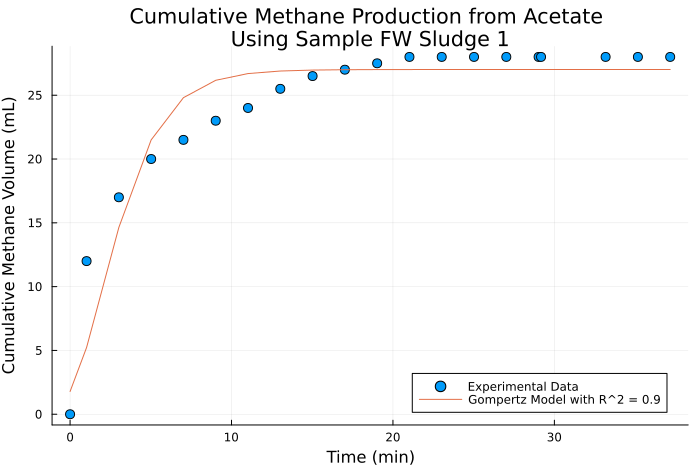
\includegraphics[width=.9\linewidth]{../plots/BMPs/Acetate/methane_kinetics_acet_test_fw_s1_min.png}
\end{center}

\begin{center}
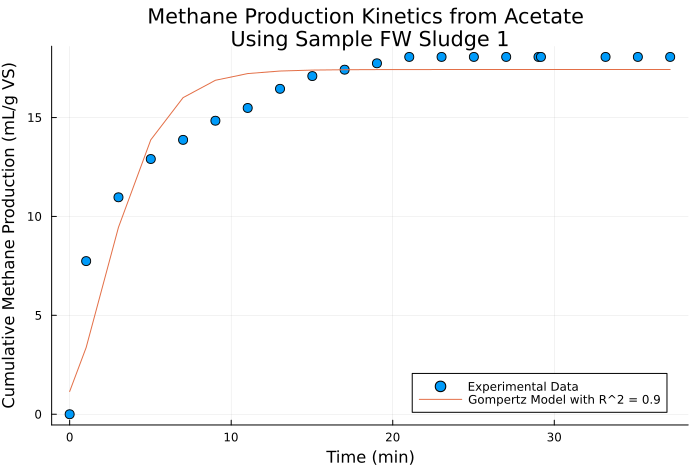
\includegraphics[width=.9\linewidth]{../plots/BMPs/Acetate/specific_methane_kinetics_acet_test_fw_s1.png}
\end{center}

\subsection{Acetate Test 0}
\label{sec:org964a24a}
Το section αυτό αναφέρεται στη δοκιμή με 100 μL οξικό στο δείγμα (0).

\textbf{acet\textsubscript{test}\textsubscript{0}\textsubscript{s1}}
\begin{minted}[breaklines=true,breakanywhere=true]{julia}

### Data Analysis on Reactor 0 ###

<<date_saving_acetate_s1>>

inds = 34:58
exp_meth_vol = [0, 4, 12, 7.5, 4.5, 2.5, 2.5, 4, 0.5, 2, 2, 1, 1, 1, 1, 1, 0.5, 0.5, 0, 0, 0, 0, 0, 0, 0]
meth_vol_acet_0 = cumsum(exp_meth_vol)[end]
exp_name = "acet_test_0_s1"
source = "Acetate"
reactor = "Reactor 0"
sludge = "Sludge 1"
run_num = "Run 1"
input_vs = 1.55
p0 = [40.0, 8.0, 1.0]

<<bmp_data_processing>>
max_rate_acet_0 = max_manual_rate

<<bmp_curve_fitting_min>>
model_acet_0 = vcat(reactor, round.(model_params, digits = 3), round(r_squared, digits = 3))
<<bmp_data_plotting>>

p0 = [25.8, 5.0, 1.0]    
<<sma_curve_fitting_min>>
sma_acet_0 = vcat(reactor, round.(model_params, digits = 3), round(r_squared, digits = 3))
<<bmp_data_plotting>>

return("../data/exp_pro/"*exp_name*".csv")
\end{minted}

\begin{minted}[breaklines=true,breakanywhere=true]{elisp}
(org-table-import-after-n-lines 4 <<acet_test_0_s1()>> '(4))
\end{minted}

\begin{table}[htbp]
\caption{Κινητικά δεδομένα}
\centering
\begin{tabular}{lrrrr}
Timestamp & Seconds & Minutes & Methane\textsubscript{Volume} & Cumulative\textsubscript{Methane}\textsubscript{Volume}\\[0pt]
29/03\textsubscript{12}:23 & 0.0 & 0.0 & 0.0 & 0.0\\[0pt]
29/03\textsubscript{12}:23 & 13.967 & 0.2328 & 4.0 & 4.0\\[0pt]
29/03\textsubscript{12}:24 & 73.986 & 1.2331 & 12.0 & 16.0\\[0pt]
29/03\textsubscript{12}:25 & 133.981 & 2.233 & 7.5 & 23.5\\[0pt]
29/03\textsubscript{12}:26 & 193.993 & 3.2332 & 4.5 & 28.0\\[0pt]
29/03\textsubscript{12}:27 & 230.339 & 3.839 & 2.5 & 30.5\\[0pt]
29/03\textsubscript{12}:28 & 290.327 & 4.8388 & 2.5 & 33.0\\[0pt]
29/03\textsubscript{12}:29 & 350.322 & 5.8387 & 4.0 & 37.0\\[0pt]
29/03\textsubscript{12}:29 & 363.719 & 6.062 & 0.5 & 37.5\\[0pt]
29/03\textsubscript{12}:30 & 423.727 & 7.0621 & 2.0 & 39.5\\[0pt]
29/03\textsubscript{12}:31 & 483.722 & 8.062 & 2.0 & 41.5\\[0pt]
29/03\textsubscript{12}:32 & 509.669 & 8.4945 & 1.0 & 42.5\\[0pt]
29/03\textsubscript{12}:33 & 569.668 & 9.4945 & 1.0 & 43.5\\[0pt]
29/03\textsubscript{12}:34 & 629.657 & 10.4943 & 1.0 & 44.5\\[0pt]
29/03\textsubscript{12}:35 & 689.661 & 11.4944 & 1.0 & 45.5\\[0pt]
29/03\textsubscript{12}:36 & 749.66 & 12.4943 & 1.0 & 46.5\\[0pt]
29/03\textsubscript{12}:37 & 809.683 & 13.4947 & 0.5 & 47.0\\[0pt]
29/03\textsubscript{12}:38 & 869.926 & 14.4988 & 0.5 & 47.5\\[0pt]
29/03\textsubscript{12}:38 & 910.87 & 15.1812 & 0.0 & 47.5\\[0pt]
29/03\textsubscript{12}:39 & 970.864 & 16.1811 & 0.0 & 47.5\\[0pt]
29/03\textsubscript{12}:40 & 1030.875 & 17.1812 & 0.0 & 47.5\\[0pt]
29/03\textsubscript{12}:41 & 1090.872 & 18.1812 & 0.0 & 47.5\\[0pt]
29/03\textsubscript{12}:42 & 1150.882 & 19.1814 & 0.0 & 47.5\\[0pt]
29/03\textsubscript{12}:43 & 1205.994 & 20.0999 & 0.0 & 47.5\\[0pt]
29/03\textsubscript{12}:44 & 1265.223 & 21.087 & 0.0 & 47.5\\[0pt]
\end{tabular}
\end{table}

\begin{center}
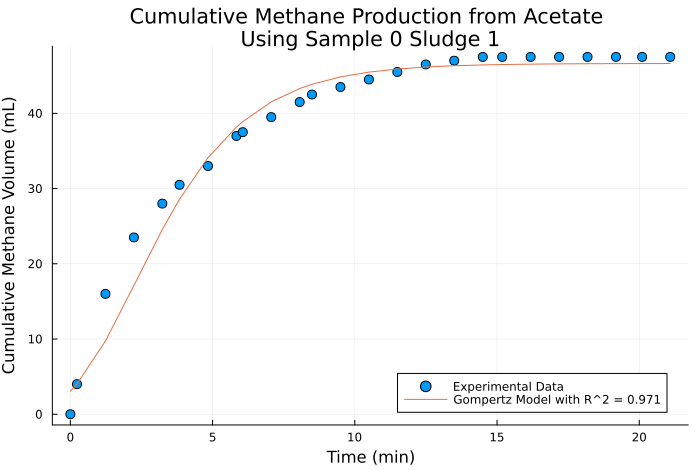
\includegraphics[width=.9\linewidth]{../plots/BMPs/Acetate/methane_kinetics_acet_test_0_s1_min.png}
\end{center}

\begin{center}
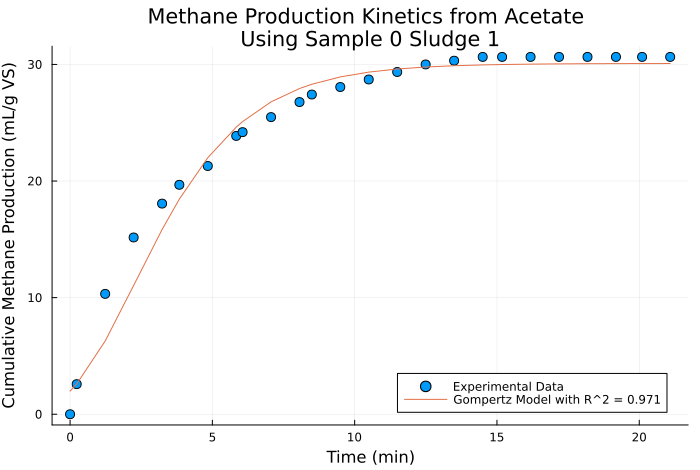
\includegraphics[width=.9\linewidth]{../plots/BMPs/Acetate/specific_methane_kinetics_acet_test_0_s1.png}
\end{center}

\subsection{Acetate Test 1}
\label{sec:org4b95f4f}
Το section αυτό αναφέρεται στη δοκιμή με 100 μL οξικό στο δείγμα (1). Aξίζει να αναφερθεί πως την πρώτη πειραματική ημέρα (27/03), παρήγαγε αέριο χωρίς να τροφοδοτηθεί με κάποιο υπόστρωμα. Η κινητική αυτής της παραγωγής (η οποία δεν ξέρουμε σε τι ευθύνεται) θα αναλυθεί παρακάτω. Βέβαια, μόλις τροφοδοτήθηκε με οξικό και η παραγωγή του τελείωσε, σταμάτησε και εκείνη η παραγωγή. Βέβαια, είχε την χαμηλότερη παραγωγή βιοαερίου μόλις τροφοδοτήθηκε με οξικό, οπότε ενδέχεται αυτή η μέτρηση να ήταν προβληματική.

\textbf{acet\textsubscript{test}\textsubscript{1}\textsubscript{s1}}
\begin{minted}[breaklines=true,breakanywhere=true]{julia}

### Data Analysis on Reactor 1 ###

<<date_saving_acetate_s1>>

inds = 38:58
exp_meth_vol = [0, 6.5, 5, 3, 0.5, 1.5, 1.5, 0.5, 1, 0.5, 0.5, 0.3, 0.2, 0.2, 0.1, 0.05, 0.05, 0.05, 0.05, 0, 0]
meth_vol_acet_1 = cumsum(exp_meth_vol)[end]
exp_name = "acet_test_1_s1"
source = "Acetate"
reactor = "Reactor 1"
sludge = "Sludge 1"
run_num = "Run 1"
input_vs = 1.55
p0 = [20.0, 4.0, 1.0]

<<bmp_data_processing>>
max_rate_acet_1 = max_manual_rate

<<bmp_curve_fitting_min>>
model_acet_1 = vcat(reactor, round.(model_params, digits = 3), round(r_squared, digits = 3))
<<bmp_data_plotting>>

p0 = [13.5, 3.5, 1.0]
<<sma_curve_fitting_min>>
sma_acet_1 = vcat(reactor, round.(model_params, digits = 3), round(r_squared, digits = 3))
<<bmp_data_plotting>>

return("../data/exp_pro/"*exp_name*".csv")
\end{minted}

\begin{minted}[breaklines=true,breakanywhere=true]{elisp}
(org-table-import-after-n-lines 4 <<acet_test_1_s1()>> '(4))
\end{minted}

\begin{table}[htbp]
\caption{Κινητικά δεδομένα}
\centering
\begin{tabular}{lrrrr}
Timestamp & Seconds & Minutes & Methane\textsubscript{Volume} & Cumulative\textsubscript{Methane}\textsubscript{Volume}\\[0pt]
\hline
29/03\textsubscript{12}:26 & 0.0 & 0.0 & 0.0 & 0.0\\[0pt]
29/03\textsubscript{12}:27 & 36.346 & 0.6058 & 6.5 & 6.5\\[0pt]
29/03\textsubscript{12}:28 & 96.334 & 1.6056 & 5.0 & 11.5\\[0pt]
29/03\textsubscript{12}:29 & 156.329 & 2.6055 & 3.0 & 14.5\\[0pt]
29/03\textsubscript{12}:29 & 169.726 & 2.8288 & 0.5 & 15.0\\[0pt]
29/03\textsubscript{12}:30 & 229.734 & 3.8289 & 1.5 & 16.5\\[0pt]
29/03\textsubscript{12}:31 & 289.729 & 4.8288 & 1.5 & 18.0\\[0pt]
29/03\textsubscript{12}:32 & 315.676 & 5.2613 & 0.5 & 18.5\\[0pt]
29/03\textsubscript{12}:33 & 375.675 & 6.2613 & 1.0 & 19.5\\[0pt]
29/03\textsubscript{12}:34 & 435.664 & 7.2611 & 0.5 & 20.0\\[0pt]
29/03\textsubscript{12}:35 & 495.668 & 8.2611 & 0.5 & 20.5\\[0pt]
29/03\textsubscript{12}:36 & 555.667 & 9.2611 & 0.3 & 20.8\\[0pt]
29/03\textsubscript{12}:37 & 615.69 & 10.2615 & 0.2 & 21.0\\[0pt]
29/03\textsubscript{12}:38 & 675.933 & 11.2656 & 0.2 & 21.2\\[0pt]
29/03\textsubscript{12}:38 & 716.877 & 11.948 & 0.1 & 21.3\\[0pt]
29/03\textsubscript{12}:39 & 776.871 & 12.9479 & 0.05 & 21.35\\[0pt]
29/03\textsubscript{12}:40 & 836.882 & 13.948 & 0.05 & 21.4\\[0pt]
29/03\textsubscript{12}:41 & 896.879 & 14.948 & 0.05 & 21.45\\[0pt]
29/03\textsubscript{12}:42 & 956.889 & 15.9482 & 0.05 & 21.5\\[0pt]
29/03\textsubscript{12}:43 & 1012.001 & 16.8667 & 0.0 & 21.5\\[0pt]
29/03\textsubscript{12}:44 & 1071.23 & 17.8538 & 0.0 & 21.5\\[0pt]
\end{tabular}
\end{table}

\begin{center}
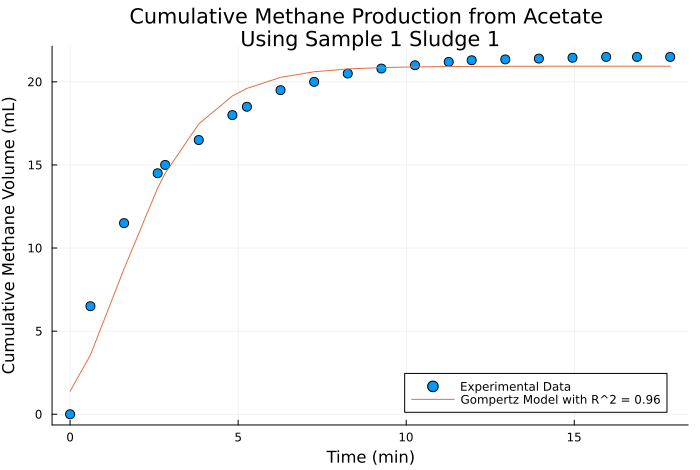
\includegraphics[width=.9\linewidth]{../plots/BMPs/Acetate/methane_kinetics_acet_test_1_s1_min.png}
\end{center}

\begin{center}
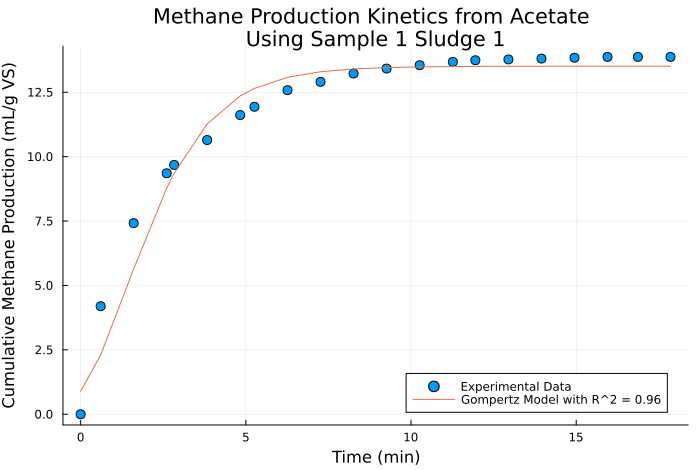
\includegraphics[width=.9\linewidth]{../plots/BMPs/Acetate/specific_methane_kinetics_acet_test_1_s1.png}
\end{center}

\subsection{Acetate Test 2}
\label{sec:org3a4980c}
Το section αυτό αναφέρεται στη δοκιμή με 100 μL οξικό στο δείγμα (2).

\textbf{acet\textsubscript{test}\textsubscript{2}\textsubscript{s1}}
\begin{minted}[breaklines=true,breakanywhere=true]{julia}

### Data Analysis on Reactor 2 ###

<<date_saving_acetate_s1>>

inds = 44:58
exp_meth_vol = [0, 4, 7, 5.5, 4.5, 2.5, 2, 1, 1, 1, 0.5, 0.5, 0.45, 0.05, 0]
meth_vol_acet_2 = cumsum(exp_meth_vol)[end]
exp_name = "acet_test_2_s1"
source = "Acetate"
reactor = "Reactor 2"
sludge = "Sludge 1"
run_num = "Run 1"
input_vs = 1.55
p0 = [30.0, 6.0, 1.0]

<<bmp_data_processing>>
max_rate_acet_2 = max_manual_rate

<<bmp_curve_fitting_min>>
model_acet_2 = vcat(reactor, round.(model_params, digits = 3), round(r_squared, digits = 3))
<<bmp_data_plotting>>

<<sma_curve_fitting_min>>
sma_acet_2 = vcat(reactor, round.(model_params, digits = 3), round(r_squared, digits = 3))
<<bmp_data_plotting>>

return("../data/exp_pro/"*exp_name*".csv")
\end{minted}

\begin{minted}[breaklines=true,breakanywhere=true]{elisp}
(org-table-import-after-n-lines 4 <<acet_test_2_s1()>> '(4))
\end{minted}

\begin{table}[htbp]
\caption{Κινητικά Δεδομένα}
\centering
\begin{tabular}{lrrrr}
Timestamp & Seconds & Minutes & Methane\textsubscript{Volume} & Cumulative\textsubscript{Methane}\textsubscript{Volume}\\[0pt]
\hline
29/03\textsubscript{12}:31 & 0.0 & 0.0 & 0.0 & 0.0\\[0pt]
29/03\textsubscript{12}:32 & 25.947 & 0.4324 & 4.0 & 4.0\\[0pt]
29/03\textsubscript{12}:33 & 85.946 & 1.4324 & 7.0 & 11.0\\[0pt]
29/03\textsubscript{12}:34 & 145.935 & 2.4322 & 5.5 & 16.5\\[0pt]
29/03\textsubscript{12}:35 & 205.939 & 3.4323 & 4.5 & 21.0\\[0pt]
29/03\textsubscript{12}:36 & 265.938 & 4.4323 & 2.5 & 23.5\\[0pt]
29/03\textsubscript{12}:37 & 325.961 & 5.4327 & 2.0 & 25.5\\[0pt]
29/03\textsubscript{12}:38 & 386.204 & 6.4367 & 1.0 & 26.5\\[0pt]
29/03\textsubscript{12}:38 & 427.148 & 7.1191 & 1.0 & 27.5\\[0pt]
29/03\textsubscript{12}:39 & 487.142 & 8.119 & 1.0 & 28.5\\[0pt]
29/03\textsubscript{12}:40 & 547.153 & 9.1192 & 0.5 & 29.0\\[0pt]
29/03\textsubscript{12}:41 & 607.15 & 10.1192 & 0.5 & 29.5\\[0pt]
29/03\textsubscript{12}:42 & 667.16 & 11.1193 & 0.45 & 29.95\\[0pt]
29/03\textsubscript{12}:43 & 722.272 & 12.0379 & 0.05 & 30.0\\[0pt]
29/03\textsubscript{12}:44 & 781.501 & 13.025 & 0.0 & 30.0\\[0pt]
\end{tabular}
\end{table}

\begin{center}
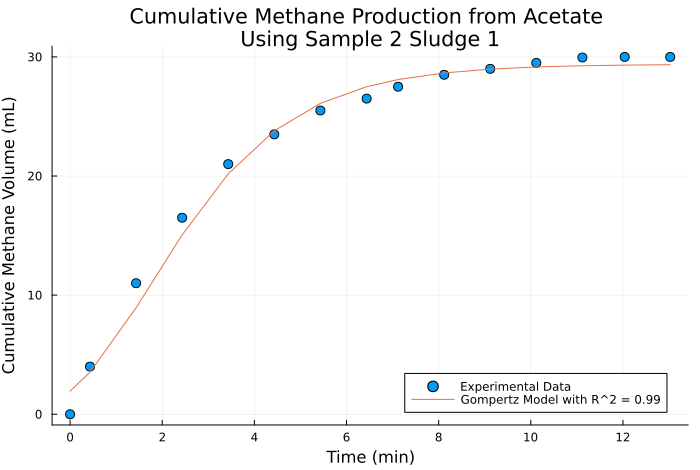
\includegraphics[width=.9\linewidth]{../plots/BMPs/Acetate/methane_kinetics_acet_test_2_s1_min.png}
\end{center}

\begin{center}
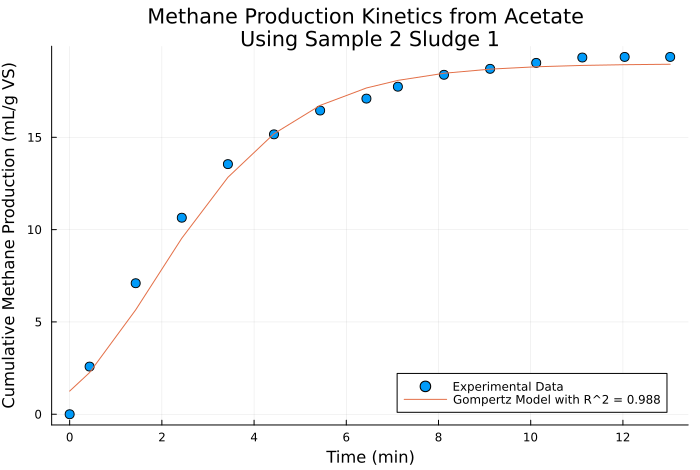
\includegraphics[width=.9\linewidth]{../plots/BMPs/Acetate/specific_methane_kinetics_acet_test_2_s1.png}
\end{center}

\subsection{Acetate Test 4}
\label{sec:org40ebdda}
Το section αυτό αναφέρεται στη δοκιμή με 100 μL οξικό στο δείγμα (4).

\textbf{acet\textsubscript{test}\textsubscript{4}\textsubscript{s1}}
\begin{minted}[breaklines=true,breakanywhere=true]{julia}

### Data Analysis on Reactor 4 ###

<<date_saving_acetate_s1>>

inds = 41:58
exp_meth_vol = [0, 4, 10, 9, 4, 5, 5, 4, 3, 3, 0, 0, 0, 0, 0, 0, 0, 0]
meth_vol_acet_4 = cumsum(exp_meth_vol)[end]
exp_name = "acet_test_4_s1"
source = "Acetate"
reactor = "Reactor 4"
sludge = "Sludge 1"
run_num = "Run 1"
input_vs = 1.55
p0 = [40.0, 10.0, 1.0]

<<bmp_data_processing>>
max_rate_acet_4 = max_manual_rate

<<bmp_curve_fitting_min>>
model_acet_4 = vcat(reactor, round.(model_params, digits = 3), round(r_squared, digits = 3))
<<bmp_data_plotting>>

<<sma_curve_fitting_min>>
sma_acet_4 = vcat(reactor, round.(model_params, digits = 3), round(r_squared, digits = 3))
<<bmp_data_plotting>>

return("../data/exp_pro/"*exp_name*".csv")
\end{minted}

\begin{minted}[breaklines=true,breakanywhere=true]{elisp}
(org-table-import-after-n-lines 4 <<acet_test_4_s1()>> '(4))
\end{minted}

\begin{table}[htbp]
\caption{Κινητικά δεδομένα}
\centering
\begin{tabular}{lrrrr}
Timestamp & Seconds & Minutes & Methane\textsubscript{Volume} & Cumulative\textsubscript{Methane}\textsubscript{Volume}\\[0pt]
\hline
29/03\textsubscript{12}:29 & 0.0 & 0.0 & 0 & 0.0\\[0pt]
29/03\textsubscript{12}:29 & 13.397 & 0.2233 & 4 & 4.0\\[0pt]
29/03\textsubscript{12}:30 & 73.405 & 1.2234 & 10 & 14.0\\[0pt]
29/03\textsubscript{12}:31 & 133.4 & 2.2233 & 9 & 23.0\\[0pt]
29/03\textsubscript{12}:32 & 159.347 & 2.6558 & 4 & 27.0\\[0pt]
29/03\textsubscript{12}:33 & 219.346 & 3.6558 & 5 & 32.0\\[0pt]
29/03\textsubscript{12}:34 & 279.335 & 4.6556 & 5 & 37.0\\[0pt]
29/03\textsubscript{12}:35 & 339.339 & 5.6556 & 4 & 41.0\\[0pt]
29/03\textsubscript{12}:36 & 399.338 & 6.6556 & 3 & 44.0\\[0pt]
29/03\textsubscript{12}:37 & 459.361 & 7.656 & 3 & 47.0\\[0pt]
29/03\textsubscript{12}:38 & 519.604 & 8.6601 & 0 & 47.0\\[0pt]
29/03\textsubscript{12}:38 & 560.548 & 9.3425 & 0 & 47.0\\[0pt]
29/03\textsubscript{12}:39 & 620.542 & 10.3424 & 0 & 47.0\\[0pt]
29/03\textsubscript{12}:40 & 680.553 & 11.3425 & 0 & 47.0\\[0pt]
29/03\textsubscript{12}:41 & 740.55 & 12.3425 & 0 & 47.0\\[0pt]
29/03\textsubscript{12}:42 & 800.56 & 13.3427 & 0 & 47.0\\[0pt]
29/03\textsubscript{12}:43 & 855.672 & 14.2612 & 0 & 47.0\\[0pt]
29/03\textsubscript{12}:44 & 914.901 & 15.2484 & 0 & 47.0\\[0pt]
\end{tabular}
\end{table}

\begin{center}
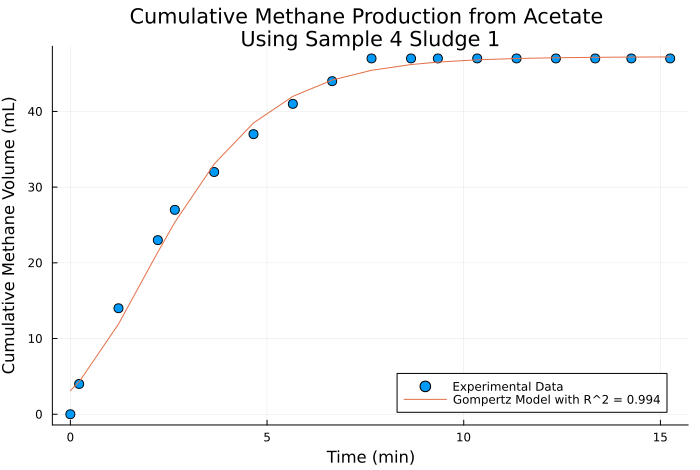
\includegraphics[width=.9\linewidth]{../plots/BMPs/Acetate/methane_kinetics_acet_test_4_s1_min.png}
\end{center}

\begin{center}
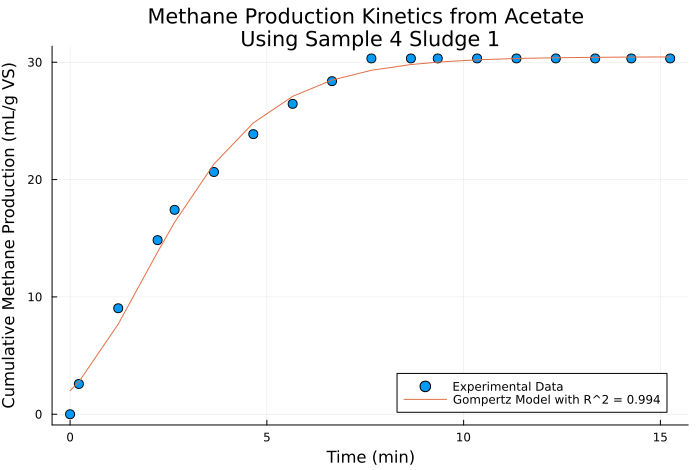
\includegraphics[width=.9\linewidth]{../plots/BMPs/Acetate/specific_methane_kinetics_acet_test_4_s1.png}
\end{center}

\subsection{Παραγωγή μεθανίου χωρίς feed από το δείγμα Ac}
\label{sec:orgbec1718}
Όπως προαναφέρθηκε, το δείγμα Ac παρήγαγε μεθάνιο χωρίς να τροφοδοτηθεί με κάτι για κάποιον ανεξήγητο λόγο. Καθώς έχουμε πειραματικά δεδομένα για αυτή την κατανάλωση (και μάλιστα 2 data sets), θα γίνει και μία ανάλυση για αυτό.

\textbf{no\textsubscript{feed}\textsubscript{ac}\textsubscript{1}}
\begin{minted}[breaklines=true,breakanywhere=true]{julia}

### No Feed Data Analysis ###

<<date_saving_acetate_s1>>

inds = 1:17
exp_meth_vol = [0, 9, 3, 2, 3, 3, 3, 2.5, 2.5, 2.5, 1.5, 3, 1, 1, 1.5, 0.5, 0.1]
exp_name = "no_feed_ac_1"
source = "No_Feed"
reactor = "Reactor Ac"
sludge = "Sludge 1"
kinetics = false

<<bmp_data_processing>>
<<bmp_data_plotting>>
\end{minted}

\textbf{no\textsubscript{feed}\textsubscript{ac}\textsubscript{2}}
\begin{minted}[breaklines=true,breakanywhere=true]{julia}

<<date_saving_acetate_s1>>

inds = 18:33
exp_meth_vol = [0, 3, 2, 2, 2, 3, 2, 2, 3, 2, 2.5, 2.5, 2, 2.5, 2.5, 2]
exp_name = "no_feed_ac_2"
source = "No_Feed"
reactor = "Reactor Ac"
sludge = "Sludge 1"
kinetics = false

<<bmp_data_processing>>
<<bmp_data_plotting>>
\end{minted}

\subsection{Update all helper}
\label{sec:orgf0967ed}
Σε αυτό το section θα υπάρχει ένα helper code block που θα κάνει evaluate όλα τα παραπάνω. Έτσι, αν αλλάξει κάτι το οποίο επηρεάζει περισσότερα από ένα code blocks, θα μπορούν να γίνουν updated ταυτόχρονα πιο εύκολα. Επίσης, μία επιπλέον χρησιμότητα του code block αυτού είναι ότι αποθηκεύει ένα CSV που συγκεντρώνει όλα τα δεδομένα των κινητικών παραμέτρων από την προσαρμογή που έγινε παραπάνω, το οποίο είναι χρήσιμο για συγκρίσεις, παρόλο που τα συγκεκριμένα πειράματα δεν είναι τόσο σημαντικό να συγκριθούν.
\textbf{update\textsubscript{acetate}\textsubscript{tests}\textsubscript{s1}}
\begin{minted}[breaklines=true,breakanywhere=true]{julia}

<<acet_test_0_s1>>
<<acet_test_1_s1>>
<<acet_test_2_s1>>
<<acet_test_4_s1>>
<<acet_test_fw_s1>>
<<no_feed_ac_1>>
<<no_feed_ac_2>>

model_fit_table = Tables.table(vcat(reshape(model_acet_0, 1, 5), reshape(model_acet_1, 1, 5), reshape(model_acet_2, 1, 5), reshape(model_acet_4, 1, 5), reshape(model_acet_fw, 1, 5)), header = [:Reactor_Name, :Production_Potential, :Production_Rate, :Lag_Time, :R_squared])
CSV.write(datadir("exp_pro", "methane_from_acetate_kinetics_s1.csv"), model_fit_table)

return("../data/exp_pro/methane_from_acetate_kinetics_s1.csv")
\end{minted}

\begin{minted}[breaklines=true,breakanywhere=true]{elisp}
(org-table-import-after-n-lines 4 <<update_acetate_tests_s1()>> '(4))
\end{minted}

\begin{table}[htbp]
\caption{Kinetic Models}
\centering
\begin{tabular}{lrrrr}
Reactor\textsubscript{Name} & Production\textsubscript{Potential} & Production\textsubscript{Rate} & Lag\textsubscript{Time} & R\textsubscript{squared}\\[0pt]
Reactor 0 & 46.633 & 7.664 & 0.0 & 0.971\\[0pt]
Reactor 1 & 20.94 & 5.448 & 0.0 & 0.96\\[0pt]
Reactor 2 & 29.389 & 6.234 & 0.0 & 0.99\\[0pt]
Reactor 4 & 47.228 & 9.65 & 0.0 & 0.994\\[0pt]
Reactor FW & 27.014 & 4.901 & 0.0 & 0.9\\[0pt]
\end{tabular}
\end{table}

\begin{minted}[breaklines=true,breakanywhere=true]{julia}

<<acet_test_0_s1>>
<<acet_test_1_s1>>
<<acet_test_2_s1>>
<<acet_test_4_s1>>
<<acet_test_fw_s1>>

sma_table = Tables.table(vcat(reshape(sma_acet_0, 1, 5), reshape(sma_acet_1, 1, 5), reshape(sma_acet_2, 1, 5), reshape(sma_acet_4, 1, 5), reshape(sma_acet_fw, 1, 5)), header = [:Reactor_Name, :Methane_Potential, :SMA, :Lag_Time, :R_sq])
CSV.write(datadir("exp_pro", "sma_from_acetate_s1.csv"), sma_table)

return("../data/exp_pro/sma_from_acetate_s1.csv")
\end{minted}

\begin{minted}[breaklines=true,breakanywhere=true]{elisp}
(org-table-import-after-n-lines 3 <<sma_acet_s1()>> '(4))
\end{minted}

\begin{center}
\begin{tabular}{lrrrr}
Reactor\textsubscript{Name} & Methane\textsubscript{Potential} & SMA & Lag\textsubscript{Time} & R\textsubscript{sq}\\[0pt]
Reactor 0 & 30.086 & 4.944 & 0.0 & 0.971\\[0pt]
Reactor 1 & 13.51 & 3.515 & 0.0 & 0.96\\[0pt]
Reactor 2 & 18.991 & 3.942 & 0.0 & 0.988\\[0pt]
Reactor 4 & 30.469 & 6.226 & 0.0 & 0.994\\[0pt]
Reactor FW & 17.428 & 3.163 & 0.0 & 0.9\\[0pt]
\end{tabular}
\end{center}

\subsection{Γενικά σχόλια για αυτόν τον κύκλο πειραμάτων}
\label{sec:orgde5376e}
Ο πρώτος αυτός κύκλος πειραμάτων ήταν για την δοκιμή προσθήκης οξικού οξέος, του ιδανικού υποστρώματος της μεθανογένεσης, για να δούμε πως θα αντιδράσει σε αυτό το σύστημα. Δεν έχει τόσο συγκριτικό χαρακτήρα μεταξύ των πειραμάτων (παρόλο που ένα σχόλιο που μπορεί να γίνει είναι πως τα πειράματα τα οποία ήταν ίδια πρακτικά στην αρχή, είχαν αρκετά διαφορετική απόκριση στην προσθήκη οξικού), αλλά τον χαρακτήρα της βέλτιστης δυνατής μεθανογένεσης από κάποιο υπόστρωμα. Από την μελέτη αυτή, προέκυψαν αρκετά συμπεράσματα.

Ένα ενδιαφέρον σχόλιο είναι πως το σύστημα ανταποκρίνεται στην προσθήκη του οξικού πολύ γρήγορα (μετά από μερικά δευτερόλεπτα κιόλας βλέπουμε παραγωγή μεθανίου) και στο μοντέλο αυτό μεταφράζεται ως μηδενικό lag-phase.

Το δείγμα 4 είχε αναπάντεχα υψηλό ρυθμό παραγωγής μεθανίου, το οποίο φάνηκε από το γεγονός ότι παράχθηκε την μέγιστη ποσότητα οξικού που περιμέναμε σε περίπου 7 λεπτά ενώ τα υπόλοιπα χρειάστηκαν τουλάχιστον 15 λεπτά. Αυτό φάνηκε και στο μοντέλο, όπου το δείγμα αυτό είχε πολύ υψηλό ειδικό ρυθμό παραγωγής μεθανίου. Το δείγμα Ac ήταν αυτό που παρήγαγε αέριο χωρίς κάποιο υπόστρωμα. Μόλις προστέθηκε οξικό, αντέδρασε σε αυτό και ο ρυθμός του αυξήθηκε, αλλά επιβράδυνε πολύ γρήγορα, με αποτέλεσμα να έχει πολύ αργό ρυθμό παραγωγής μεθανίο και το χαμηλότερο δυναμικό παραγωγής μεθανίου. Μπορεί η αλλαγή αυτή να ευθύνεται σε αυτήν την απόκριση. Τα δείγματα 0 και 4 είχαν πολύ μεγαλύτερη παραγωγικότητα από τα άλλα 3, χωρίς να υπάρχει κάποια εύκολη εξήγηση για αυτό.

\pagebreak

\section{FW Hydrolysate S1\textsubscript{R1} Processing}
\label{sec:org350c8c7}
Στο section αυτό θα αναλυθούν τα αποτελεσματα του πρώτου πειράματος που χρησιμοποιήσε FW hydrolysate ως υπόστρωμα (συμβολίζεται ως S1\textsubscript{R1} επειδή είναι το πρώτο run με την πρώτη λάσπη). Σκοπός είναι να γίνει μία σύγκριση αυτού με το οξικό για κάθε δοχείο για να προκύψουν αποτελέσματα για το κάθε πείραμα. Οι 5 δοκιμές που έγιναν ήταν στα δείγματα 0, 1, 2 και 4 (τα οποία πλέον έχουν νόημα επειδή εκφράζουν την ποσότητα mix που προστέθηκε κατά την υδρόλυση) αλλά επίσης έγινε και ένα πείραμα για να μετρηθεί η απόδοση σε μεθάνιο του δείγματος μόνο με FW.

Αξίζει να αναφερθεί πως παρατηρήθηκε μία απότομη μεταβολή της στάθμης του αερίου στην αρχή κάθε πειράματος εκτός από το FW. Αυτή αγνοήθηκε καθώς υποτέθηκε πως έγινε λόγω διαφοράς πίεσης κατά την διαδικασία της τροφοδοσίας. Αυτό μπορεί να οδηγεί σε κάποιο σφάλμα, αλλά αν δεν αγνοηθεί οδηγεί σε πολύ προβληματικά αποτελέσματα.

\subsection{Reactor 0}
\label{sec:org7922370}
Το δείγμα αυτό είναι labelled ως δείγμα 0 καθώς είναι το δείγμα το οποίο τροφοδοτήθηκε με treated FW, όμως χωρίς προσθήκη του μιξ ενζύμων και μικροοργανισμών. Όπως έχουμε δεί, όλες οι αντιδράσεις που γίνονται κατά την υδρόλυση και ζύμωση μπορούν να γίνουν και χωρίς το μιξ. Όμως, γινόντουσαν πιο αποτελεσματικά με την προσθήκη αυτού. Οπότε, ελπίζουμε πως το δείγμα αυτό θα έχει χειρότερα αποτελέσματα από τα άλλα, το οποίο θα μας οδηγήσει στην υπόθεση ότι το μιξ βελτιώνει όχι μόνο τα κριτήρια υδρόλυσης και οξεογένεσης αλλά και αυτό της μεθανογένεσης.

\textbf{hydrolysate\textsubscript{0}\textsubscript{s1}\textsubscript{r1}}
\begin{minted}[breaklines=true,breakanywhere=true]{julia}

### Data Analysis on Hydrolysate with 0 ml ###

<<date_saving_fw_s1_r1>>

inds = 3:50
exp_meth_vol = [0, 0, 0, 0, 0, 0, 0.1, 0.1, 0.1, 0.2, 0.1, 0.05, 0.05, 0.1, 0.1, 0.05, 0.1, 0.1, 0.1, 0.2, 0.3, 0.1, 0.1, 0.1, 0.1, 0.1, 0, 0, 0, 0, 0.2, 0.2, 0.1, 0.1, 0.1, 0.1, 0.1, 0.2, 0.3, 0.2, 0.1, 0.1, 0.1, 0.0, 0.0, 0.0, 0.0, 0.0]
meth_vol_hydro_0 = cumsum(exp_meth_vol)[end]

exp_name = "hydrolysate_0_s1_r1"
source = "Hydrolyzed FW"
reactor = "Reactor 0"
sludge = "Sludge 1"
run_num = "Run 1"
input_vs = 1.55

<<bmp_data_processing>>
max_rate_hydro_0 = max_manual_rate

# The same model is fit either with min or hour
p0 = [6.0, 0.01, 1.0]
<<bmp_curve_fitting_min>>
model_hydro_0_min = vcat(reactor, round.(model_params, digits = 3), round(r_squared, digits = 3))
<<bmp_data_plotting>>

p0 = [6.0, 0.2, 1.0]
<<bmp_curve_fitting_hour>>
model_hydro_0_hour = vcat(reactor, round.(model_params, digits = 3), round(r_squared, digits = 3))
<<bmp_data_plotting>>

p0 = [6.0, 0.1, 1.0]
<<sma_curve_fitting_hour>>
sma_hydro_0 = vcat(reactor, round.(model_params, digits = 3), round(r_squared, digits = 3))
<<bmp_data_plotting>>

return("../data/exp_pro/"*exp_name*".csv")
\end{minted}

\subsubsection{Results}
\label{sec:orgb4cd610}
Παρακάτω φαίνονται τα αποτελέσματα του σχετικού πειράματος.

\begin{minted}[breaklines=true,breakanywhere=true]{elisp}
(org-table-import-after-n-lines 3 <<hydrolysate_0_s1_r1()>> '(4))
\end{minted}

\begin{center}
\begin{tabular}{lrrrr}
Timestamp & Minutes & Hours & Methane\textsubscript{Volume} & Cumulative\textsubscript{Methane}\textsubscript{Volume}\\[0pt]
01/04\textsubscript{11}:11 & 0.0 & 0.0 & 0.0 & 0.0\\[0pt]
01/04\textsubscript{11}:12 & 1.0002 & 0.0167 & 0.0 & 0.0\\[0pt]
01/04\textsubscript{11}:13 & 1.8288 & 0.0305 & 0.0 & 0.0\\[0pt]
01/04\textsubscript{11}:14 & 2.8286 & 0.0471 & 0.0 & 0.0\\[0pt]
01/04\textsubscript{11}:15 & 3.8288 & 0.0638 & 0.0 & 0.0\\[0pt]
01/04\textsubscript{11}:21 & 10.2674 & 0.1711 & 0.0 & 0.0\\[0pt]
01/04\textsubscript{11}:52 & 40.5936 & 0.6766 & 0.1 & 0.1\\[0pt]
01/04\textsubscript{12}:22 & 70.5935 & 1.1766 & 0.1 & 0.2\\[0pt]
01/04\textsubscript{13}:52 & 160.5938 & 2.6766 & 0.1 & 0.3\\[0pt]
01/04\textsubscript{15}:52 & 280.5938 & 4.6766 & 0.2 & 0.5\\[0pt]
01/04\textsubscript{16}:52 & 340.5941 & 5.6766 & 0.1 & 0.6\\[0pt]
01/04\textsubscript{18}:52 & 460.5922 & 7.6765 & 0.05 & 0.65\\[0pt]
01/04\textsubscript{20}:52 & 580.5921 & 9.6765 & 0.05 & 0.7\\[0pt]
01/04\textsubscript{22}:52 & 700.5956 & 11.6766 & 0.1 & 0.8\\[0pt]
02/04\textsubscript{00}:52 & 820.6106 & 13.6768 & 0.1 & 0.9\\[0pt]
02/04\textsubscript{02}:52 & 940.6072 & 15.6768 & 0.05 & 0.95\\[0pt]
02/04\textsubscript{04}:52 & 1060.6068 & 17.6768 & 0.1 & 1.05\\[0pt]
02/04\textsubscript{06}:52 & 1180.6299 & 19.6772 & 0.1 & 1.15\\[0pt]
02/04\textsubscript{08}:52 & 1300.585 & 21.6764 & 0.1 & 1.25\\[0pt]
02/04\textsubscript{10}:54 & 1422.4049 & 23.7067 & 0.2 & 1.45\\[0pt]
02/04\textsubscript{12}:54 & 1542.4123 & 25.7069 & 0.3 & 1.75\\[0pt]
02/04\textsubscript{13}:24 & 1572.4122 & 26.2069 & 0.1 & 1.85\\[0pt]
02/04\textsubscript{13}:54 & 1602.4124 & 26.7069 & 0.1 & 1.95\\[0pt]
02/04\textsubscript{14}:24 & 1632.4124 & 27.2069 & 0.1 & 2.05\\[0pt]
02/04\textsubscript{14}:54 & 1662.4124 & 27.7069 & 0.1 & 2.15\\[0pt]
02/04\textsubscript{15}:24 & 1692.4122 & 28.2069 & 0.1 & 2.25\\[0pt]
02/04\textsubscript{15}:54 & 1722.4122 & 28.7069 & 0.0 & 2.25\\[0pt]
02/04\textsubscript{16}:24 & 1752.4125 & 29.2069 & 0.0 & 2.25\\[0pt]
02/04\textsubscript{16}:54 & 1782.4125 & 29.7069 & 0.0 & 2.25\\[0pt]
02/04\textsubscript{17}:24 & 1812.4122 & 30.2069 & 0.0 & 2.25\\[0pt]
02/04\textsubscript{17}:54 & 1842.419 & 30.707 & 0.2 & 2.45\\[0pt]
02/04\textsubscript{19}:54 & 1962.4195 & 32.707 & 0.2 & 2.65\\[0pt]
02/04\textsubscript{21}:54 & 2082.4211 & 34.707 & 0.1 & 2.75\\[0pt]
02/04\textsubscript{23}:54 & 2202.4254 & 36.7071 & 0.1 & 2.85\\[0pt]
03/04\textsubscript{01}:54 & 2322.4254 & 38.7071 & 0.1 & 2.95\\[0pt]
03/04\textsubscript{03}:54 & 2442.4252 & 40.7071 & 0.1 & 3.05\\[0pt]
03/04\textsubscript{05}:54 & 2562.4302 & 42.7072 & 0.1 & 3.15\\[0pt]
03/04\textsubscript{07}:54 & 2682.4321 & 44.7072 & 0.2 & 3.35\\[0pt]
03/04\textsubscript{09}:54 & 2802.4322 & 46.7072 & 0.3 & 3.65\\[0pt]
03/04\textsubscript{12}:54 & 2982.4411 & 49.7074 & 0.2 & 3.85\\[0pt]
03/04\textsubscript{13}:54 & 3042.4409 & 50.7073 & 0.1 & 3.95\\[0pt]
03/04\textsubscript{14}:24 & 3072.4419 & 51.2074 & 0.1 & 4.05\\[0pt]
03/04\textsubscript{14}:54 & 3103.2005 & 51.72 & 0.1 & 4.15\\[0pt]
03/04\textsubscript{15}:26 & 3135.2464 & 52.2541 & 0.0 & 4.15\\[0pt]
03/04\textsubscript{16}:29 & 3197.5173 & 53.292 & 0.0 & 4.15\\[0pt]
03/04\textsubscript{17}:29 & 3257.5217 & 54.292 & 0.0 & 4.15\\[0pt]
03/04\textsubscript{18}:29 & 3317.5217 & 55.292 & 0.0 & 4.15\\[0pt]
03/04\textsubscript{20}:29 & 3437.5217 & 57.292 & 0.0 & 4.15\\[0pt]
\end{tabular}
\end{center}

\begin{center}
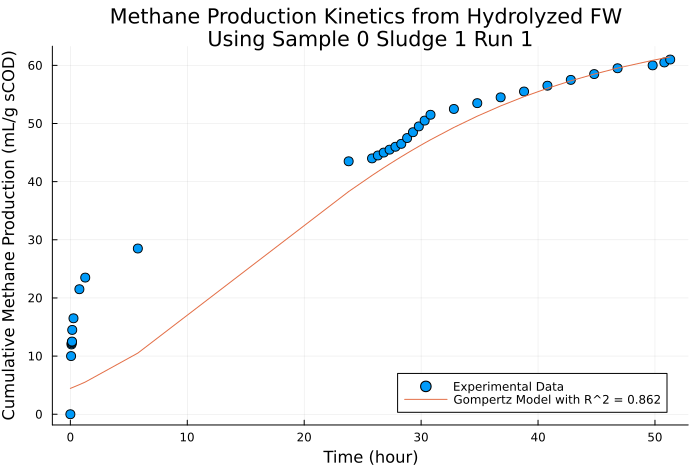
\includegraphics[width=.9\linewidth]{../plots/BMPs/Hydrolyzed FW/methane_kinetics_hydrolysate_0_s1_r1_hour.png}
\end{center}

\begin{center}
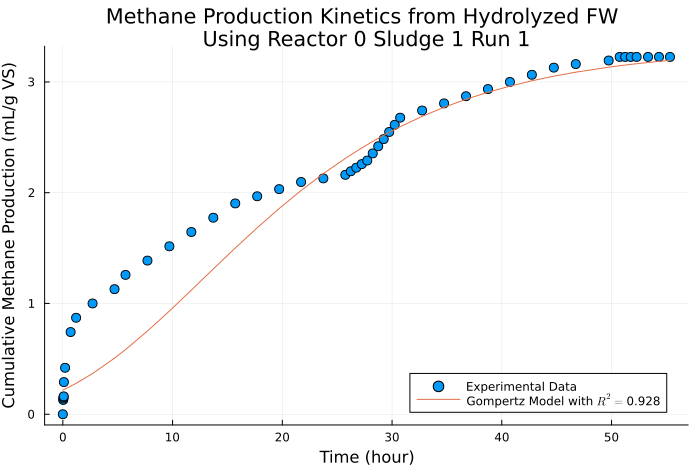
\includegraphics[width=.9\linewidth]{../plots/BMPs/Hydrolyzed FW/specific_methane_kinetics_hydrolysate_0_s1_r1_hour.png}
\end{center}

\subsection{Reactor 1}
\label{sec:org2e00e3d}
Το δείγμα αυτό τροφοδοτήθηκε με το υδρόλυμα το οποίο είχε προσθήκη 1 ml mix. Στο αρχικό κινητικό πείραμα, το δείγμα αυτό είχε αρκετά παρόμοια συμπεριφορά με το 0 και χειρότερη αυτής του 1. Από την μέτρηση του COD του, είχε αναπάντεχα υψηλό sCOD. Αυτό σημαίνει είτε πως έγινε κάποιο λάθος στην ανάλυση ή ότι απλώς έγινε πολύ καλύτερη υδρόλυση από ότι περιμέναμε στο πείραμα αυτό. Με βάση το sCOD του, αναμένεται να έχει καλά αποτελέσματα. Με βάση την HPLC του αρχικού πειράματος, θα περιμέναμε να είναι λίγο καλύτερο από το 0.

\textbf{hydrolysate\textsubscript{1}\textsubscript{s1}\textsubscript{r1}}
\begin{minted}[breaklines=true,breakanywhere=true]{julia}

### Data Analysis on Hydrolysate with 1 ml ###

<<date_saving_fw_s1_r1>>

inds = 3:49
exp_meth_vol = [0, 0.05, 0.05, 0.1, 0.2, 0.2, 0.2, 0.2, 0.3, 0.1, 0.2, 0.2, 0.2, 0.3, 0.4, 0.4, 0.3, 0.4, 0.4, 0.3, 0.2, 0.3, 0.3, 0.3, 0.3, 0.2, 0.3, 0.3, 0.4, 0.5, 0.4, 0.3, 0.3, 0.3, 0.2, 0.2, 0.1, 0.1, 0.1, 0.05, 0.05, 0, 0, 0, 0, 0, 0]
meth_vol_hydro_1 = cumsum(exp_meth_vol)[end]
exp_name = "hydrolysate_1_s1_r1"
source = "Hydrolyzed FW"
reactor = "Reactor 1"
sludge = "Sludge 1"
run_num = "Run 1"
input_vs = 1.55

p0 = [13.0, 0.1, 1.0]
<<bmp_data_processing>>
max_rate_hydro_1 = max_manual_rate

<<bmp_curve_fitting_min>>
model_hydro_1_min = vcat(reactor, round.(model_params, digits = 3), round(r_squared, digits = 3))
<<bmp_data_plotting>>

p0 = [13.0, 1.0, 1.0]
<<bmp_curve_fitting_hour>>
model_hydro_1_hour = vcat(reactor, round.(model_params, digits = 3), round(r_squared, digits = 3))
<<bmp_data_plotting>>

<<sma_curve_fitting_hour>>
sma_hydro_1 = vcat(reactor, round.(model_params, digits = 3), round(r_squared, digits = 3))
<<bmp_data_plotting>>

return("../data/exp_pro/"*exp_name*".csv")
\end{minted}

\subsubsection{Results}
\label{sec:orgf446da9}
Το πείραμα αυτό παρήγαγε 10.95 ml μεθάνιο, το οποίο είναι το \(50.93 \%\) του πειράματος με οξικό καθώς εκείνο το πείραμα είχε μία σχετικά χαμηλή παραγωγικότητα για οξικό.

Από άποψη προσαρμογής, το πείραμα αυτό έχει το πρόβλημα πως η παραγωγή μεθανίου φαίνεται να πηγαίνει με "σκαλοπατάκια". Για κάποια διαστήματα πηγαίνει πολύ γρήγορα, ενώ μετά πηγαίνει αργά. Αυτό συμβαίνει μερικές ώρες μετά την έναρξη, ξαναεπιταχύνει λίγο μετά το 24ωρο και λίγο πριν το τέλος της χώνευσης (στις 49 ώρες), ξαναεπιταχύνει για λίγο. Οπότε, η προσαρμογή του είναι αρκετά δύσκολη.

Με την διόρθωση των δεδομένων σταματάει να υπάρχει το φαινόμενο των 2 ρυθμών (ενός γρήγορου για τα δείγματα της 1ης μέρας και ενός αργού για μετά), αλλά η προσαρμογή ακόμη δεν είναι τέλεια (παρότι είναι πλέον αρκετά καλή)

\begin{minted}[breaklines=true,breakanywhere=true]{elisp}
(org-table-import-after-n-lines 3 <<hydrolysate_1_s1_r1()>> '(4))
\end{minted}

\begin{center}
\begin{tabular}{lrrrr}
Timestamp & Minutes & Hours & Methane\textsubscript{Volume} & Cumulative\textsubscript{Methane}\textsubscript{Volume}\\[0pt]
01/04\textsubscript{11}:11 & 0.0 & 0.0 & 0.0 & 0.0\\[0pt]
01/04\textsubscript{11}:12 & 1.0002 & 0.0167 & 0.05 & 0.05\\[0pt]
01/04\textsubscript{11}:13 & 1.8288 & 0.0305 & 0.05 & 0.1\\[0pt]
01/04\textsubscript{11}:14 & 2.8286 & 0.0471 & 0.1 & 0.2\\[0pt]
01/04\textsubscript{11}:15 & 3.8288 & 0.0638 & 0.2 & 0.4\\[0pt]
01/04\textsubscript{11}:21 & 10.2674 & 0.1711 & 0.2 & 0.6\\[0pt]
01/04\textsubscript{11}:52 & 40.5936 & 0.6766 & 0.2 & 0.8\\[0pt]
01/04\textsubscript{12}:22 & 70.5935 & 1.1766 & 0.2 & 1.0\\[0pt]
01/04\textsubscript{13}:52 & 160.5938 & 2.6766 & 0.3 & 1.3\\[0pt]
01/04\textsubscript{15}:52 & 280.5938 & 4.6766 & 0.1 & 1.4\\[0pt]
01/04\textsubscript{16}:52 & 340.5941 & 5.6766 & 0.2 & 1.6\\[0pt]
01/04\textsubscript{18}:52 & 460.5922 & 7.6765 & 0.2 & 1.8\\[0pt]
01/04\textsubscript{20}:52 & 580.5921 & 9.6765 & 0.2 & 2.0\\[0pt]
01/04\textsubscript{22}:52 & 700.5956 & 11.6766 & 0.3 & 2.3\\[0pt]
02/04\textsubscript{00}:52 & 820.6106 & 13.6768 & 0.4 & 2.7\\[0pt]
02/04\textsubscript{02}:52 & 940.6072 & 15.6768 & 0.4 & 3.1\\[0pt]
02/04\textsubscript{04}:52 & 1060.6068 & 17.6768 & 0.3 & 3.4\\[0pt]
02/04\textsubscript{06}:52 & 1180.6299 & 19.6772 & 0.4 & 3.8\\[0pt]
02/04\textsubscript{08}:52 & 1300.585 & 21.6764 & 0.4 & 4.2\\[0pt]
02/04\textsubscript{10}:54 & 1422.4049 & 23.7067 & 0.3 & 4.5\\[0pt]
02/04\textsubscript{12}:54 & 1542.4123 & 25.7069 & 0.2 & 4.7\\[0pt]
02/04\textsubscript{13}:24 & 1572.4122 & 26.2069 & 0.3 & 5.0\\[0pt]
02/04\textsubscript{13}:54 & 1602.4124 & 26.7069 & 0.3 & 5.3\\[0pt]
02/04\textsubscript{14}:24 & 1632.4124 & 27.2069 & 0.3 & 5.6\\[0pt]
02/04\textsubscript{14}:54 & 1662.4124 & 27.7069 & 0.3 & 5.9\\[0pt]
02/04\textsubscript{15}:24 & 1692.4122 & 28.2069 & 0.2 & 6.1\\[0pt]
02/04\textsubscript{15}:54 & 1722.4122 & 28.7069 & 0.3 & 6.4\\[0pt]
02/04\textsubscript{16}:24 & 1752.4125 & 29.2069 & 0.3 & 6.7\\[0pt]
02/04\textsubscript{16}:54 & 1782.4125 & 29.7069 & 0.4 & 7.1\\[0pt]
02/04\textsubscript{17}:24 & 1812.4122 & 30.2069 & 0.5 & 7.6\\[0pt]
02/04\textsubscript{17}:54 & 1842.419 & 30.707 & 0.4 & 8.0\\[0pt]
02/04\textsubscript{19}:54 & 1962.4195 & 32.707 & 0.3 & 8.3\\[0pt]
02/04\textsubscript{21}:54 & 2082.4211 & 34.707 & 0.3 & 8.6\\[0pt]
02/04\textsubscript{23}:54 & 2202.4254 & 36.7071 & 0.3 & 8.9\\[0pt]
03/04\textsubscript{01}:54 & 2322.4254 & 38.7071 & 0.2 & 9.1\\[0pt]
03/04\textsubscript{03}:54 & 2442.4252 & 40.7071 & 0.2 & 9.3\\[0pt]
03/04\textsubscript{05}:54 & 2562.4302 & 42.7072 & 0.1 & 9.4\\[0pt]
03/04\textsubscript{07}:54 & 2682.4321 & 44.7072 & 0.1 & 9.5\\[0pt]
03/04\textsubscript{09}:54 & 2802.4322 & 46.7072 & 0.1 & 9.6\\[0pt]
03/04\textsubscript{12}:54 & 2982.4411 & 49.7074 & 0.05 & 9.65\\[0pt]
03/04\textsubscript{13}:54 & 3042.4409 & 50.7073 & 0.05 & 9.7\\[0pt]
03/04\textsubscript{14}:24 & 3072.4419 & 51.2074 & 0.0 & 9.7\\[0pt]
03/04\textsubscript{14}:54 & 3103.2005 & 51.72 & 0.0 & 9.7\\[0pt]
03/04\textsubscript{15}:26 & 3135.2464 & 52.2541 & 0.0 & 9.7\\[0pt]
03/04\textsubscript{16}:29 & 3197.5173 & 53.292 & 0.0 & 9.7\\[0pt]
03/04\textsubscript{17}:29 & 3257.5217 & 54.292 & 0.0 & 9.7\\[0pt]
03/04\textsubscript{18}:29 & 3317.5217 & 55.292 & 0.0 & 9.7\\[0pt]
\end{tabular}
\end{center}

\begin{center}
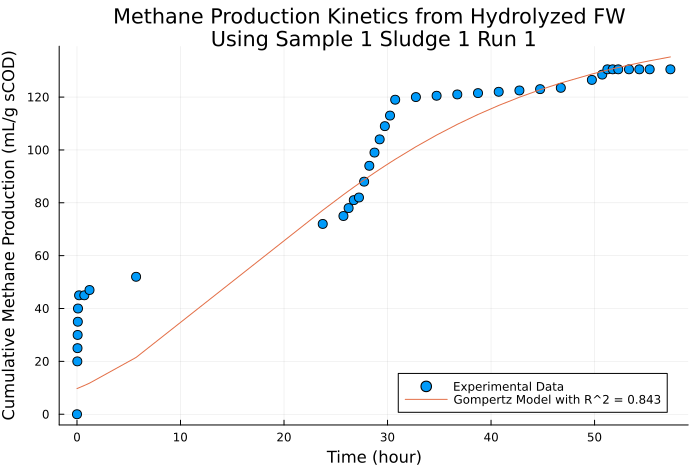
\includegraphics[width=.9\linewidth]{../plots/BMPs/Hydrolyzed FW/methane_kinetics_hydrolysate_1_s1_r1_hour.png}
\end{center}

\begin{center}
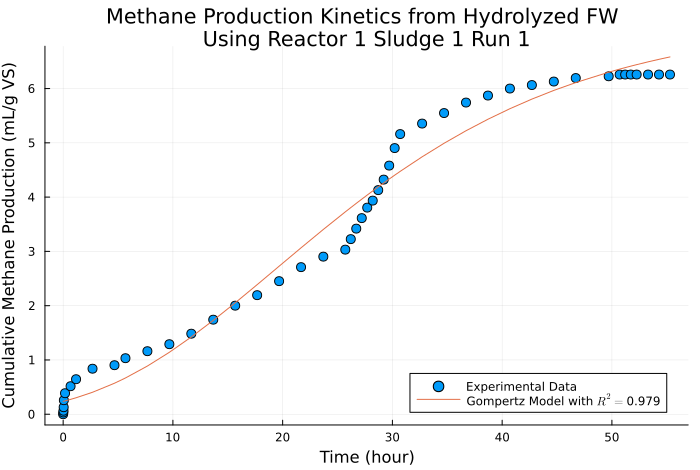
\includegraphics[width=.9\linewidth]{../plots/BMPs/Hydrolyzed FW/specific_methane_kinetics_hydrolysate_1_s1_r1_hour.png}
\end{center}

\subsection{Reactor 2}
\label{sec:orga0a2e98}
Το δείγμα το οποίο στην υδρόλυση είχε 2 ml από το μιξ. Με βάση το αρχικό πείραμα υδρόλυσης, αυτό και το 4 ml είχαν το καλύτερο performance και ελάχιστη διαφορά μεταξύ τους (κατά βάση στην συγκέντρωση γαλακτικού οξέος) οπότε θα αναμέναμε εδώ να παρατηρηθεί η καλύτερη μεθανογένεση.

\textbf{hydrolysate\textsubscript{2}\textsubscript{s1}\textsubscript{r1}}
\begin{minted}[breaklines=true,breakanywhere=true]{julia}

### Data Analysis on Hydrolysate with 2 ml ###

<<date_saving_fw_s1_r1>>

inds = 8:49
exp_meth_vol = [0, 0.2, 0.2, 0.2, 0.3, 0.3, 0.3, 0.3, 0.3, 0.3, 0.3, 0.3, 0.3, 0.3, 0.2, 0.1, 0.2, 0.2, 0.2, 0.2, 0.2, 0.2, 0.1, 0.1, 0.1, 0.1, 0.1, 0.1, 0.1, 0.1, 0.1, 0.1, 0.1, 0.1, 0.2, 0.2, 0, 0, 0, 0, 0, 0]
meth_vol_hydro_2 = cumsum(exp_meth_vol)[end]
exp_name = "hydrolysate_2_s1_r1"
source = "Hydrolyzed FW"
reactor = "Reactor 2"
sludge = "Sludge 1"
run_num = "Run 1"
input_vs = 1.55

<<bmp_data_processing>>
max_rate_hydro_2 = max_manual_rate

p0 = [10.0, 0.01, 1.0]
<<bmp_curve_fitting_min>>
model_hydro_2_min = vcat(reactor, round.(model_params, digits = 3), round(r_squared, digits = 3))
<<bmp_data_plotting>>

p0 = [10.0, 0.2, 0.03]
<<bmp_curve_fitting_hour>>
model_hydro_2_hour = vcat(reactor, round.(model_params, digits = 3), round(r_squared, digits = 3))
<<bmp_data_plotting>>

<<sma_curve_fitting_hour>>
sma_hydro_2 = vcat(reactor, round.(model_params, digits = 3), round(r_squared, digits = 3))
<<bmp_data_plotting>>

return("../data/exp_pro/"*exp_name*".csv")
\end{minted}

\subsubsection{Results}
\label{sec:org89ca61f}
Το παραγώμενο μεθάνιο είναι 5.1 ml, δηλαδή \(17 \%\) του προβλεπόμενου μεθανίου με βάση το οξικό.

\begin{enumerate}
\item Διορθωμένα αποτελέσματα
\label{sec:org6277e30}
Διορθώνοντας το μεγάλο κενό που υπήρξε στο τέλος της 01/04 και αφαιρόντας τα 6 ml που παράγονται το πρώτο λεπτό, το μοντελό αυτό διορθώνεται σε πολύ μεγάλο βαθμό. Το R\textsuperscript{2} είναι πλέον 0.98 και φαίνεται πως η προσαρμογή είναι καλή.

\begin{minted}[breaklines=true,breakanywhere=true]{elisp}
(org-table-import-after-n-lines 3 <<hydrolysate_2_s1_r1()>> '(4))
\end{minted}

\begin{center}
\begin{tabular}{lrrrr}
Timestamp & Minutes & Hours & Methane\textsubscript{Volume} & Cumulative\textsubscript{Methane}\textsubscript{Volume}\\[0pt]
01/04\textsubscript{11}:21 & 0.0 & 0.0 & 0.0 & 0.0\\[0pt]
01/04\textsubscript{11}:52 & 30.3261 & 0.5054 & 0.2 & 0.2\\[0pt]
01/04\textsubscript{12}:22 & 60.3261 & 1.0054 & 0.2 & 0.4\\[0pt]
01/04\textsubscript{13}:52 & 150.3263 & 2.5054 & 0.2 & 0.6\\[0pt]
01/04\textsubscript{15}:52 & 270.3264 & 4.5054 & 0.3 & 0.9\\[0pt]
01/04\textsubscript{16}:52 & 330.3267 & 5.5054 & 0.3 & 1.2\\[0pt]
01/04\textsubscript{18}:52 & 450.3248 & 7.5054 & 0.3 & 1.5\\[0pt]
01/04\textsubscript{20}:52 & 570.3247 & 9.5054 & 0.3 & 1.8\\[0pt]
01/04\textsubscript{22}:52 & 690.3281 & 11.5055 & 0.3 & 2.1\\[0pt]
02/04\textsubscript{00}:52 & 810.3431 & 13.5057 & 0.3 & 2.4\\[0pt]
02/04\textsubscript{02}:52 & 930.3398 & 15.5057 & 0.3 & 2.7\\[0pt]
02/04\textsubscript{04}:52 & 1050.3393 & 17.5057 & 0.3 & 3.0\\[0pt]
02/04\textsubscript{06}:52 & 1170.3624 & 19.506 & 0.3 & 3.3\\[0pt]
02/04\textsubscript{08}:52 & 1290.3175 & 21.5053 & 0.3 & 3.6\\[0pt]
02/04\textsubscript{10}:54 & 1412.1374 & 23.5356 & 0.2 & 3.8\\[0pt]
02/04\textsubscript{12}:54 & 1532.1448 & 25.5357 & 0.1 & 3.9\\[0pt]
02/04\textsubscript{13}:24 & 1562.1448 & 26.0357 & 0.2 & 4.1\\[0pt]
02/04\textsubscript{13}:54 & 1592.145 & 26.5357 & 0.2 & 4.3\\[0pt]
02/04\textsubscript{14}:24 & 1622.145 & 27.0358 & 0.2 & 4.5\\[0pt]
02/04\textsubscript{14}:54 & 1652.1449 & 27.5357 & 0.2 & 4.7\\[0pt]
02/04\textsubscript{15}:24 & 1682.1448 & 28.0357 & 0.2 & 4.9\\[0pt]
02/04\textsubscript{15}:54 & 1712.1448 & 28.5357 & 0.2 & 5.1\\[0pt]
02/04\textsubscript{16}:24 & 1742.145 & 29.0358 & 0.1 & 5.2\\[0pt]
02/04\textsubscript{16}:54 & 1772.145 & 29.5358 & 0.1 & 5.3\\[0pt]
02/04\textsubscript{17}:24 & 1802.1448 & 30.0357 & 0.1 & 5.4\\[0pt]
02/04\textsubscript{17}:54 & 1832.1516 & 30.5359 & 0.1 & 5.5\\[0pt]
02/04\textsubscript{19}:54 & 1952.1521 & 32.5359 & 0.1 & 5.6\\[0pt]
02/04\textsubscript{21}:54 & 2072.1537 & 34.5359 & 0.1 & 5.7\\[0pt]
02/04\textsubscript{23}:54 & 2192.1579 & 36.536 & 0.1 & 5.8\\[0pt]
03/04\textsubscript{01}:54 & 2312.158 & 38.536 & 0.1 & 5.9\\[0pt]
03/04\textsubscript{03}:54 & 2432.1578 & 40.536 & 0.1 & 6.0\\[0pt]
03/04\textsubscript{05}:54 & 2552.1628 & 42.536 & 0.1 & 6.1\\[0pt]
03/04\textsubscript{07}:54 & 2672.1647 & 44.5361 & 0.1 & 6.2\\[0pt]
03/04\textsubscript{09}:54 & 2792.1648 & 46.5361 & 0.1 & 6.3\\[0pt]
03/04\textsubscript{12}:54 & 2972.1736 & 49.5362 & 0.2 & 6.5\\[0pt]
03/04\textsubscript{13}:54 & 3032.1734 & 50.5362 & 0.2 & 6.7\\[0pt]
03/04\textsubscript{14}:24 & 3062.1744 & 51.0362 & 0.0 & 6.7\\[0pt]
03/04\textsubscript{14}:54 & 3092.9331 & 51.5489 & 0.0 & 6.7\\[0pt]
03/04\textsubscript{15}:26 & 3124.9789 & 52.083 & 0.0 & 6.7\\[0pt]
03/04\textsubscript{16}:29 & 3187.2498 & 53.1208 & 0.0 & 6.7\\[0pt]
03/04\textsubscript{17}:29 & 3247.2543 & 54.1209 & 0.0 & 6.7\\[0pt]
03/04\textsubscript{18}:29 & 3307.2542 & 55.1209 & 0.0 & 6.7\\[0pt]
\end{tabular}
\end{center}


\begin{center}
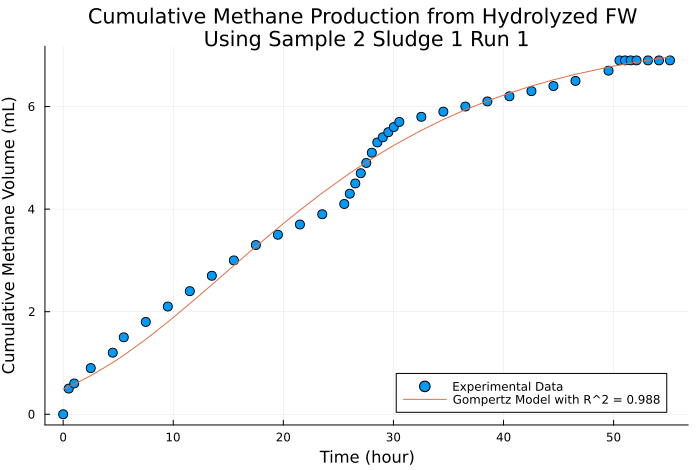
\includegraphics[width=.9\linewidth]{../plots/BMPs/Hydrolyzed FW/methane_kinetics_hydrolysate_2_s1_r1_hour.png}
\end{center}

\begin{center}
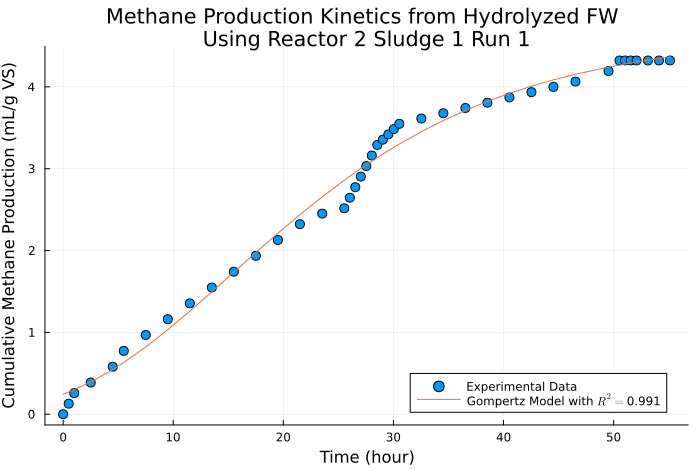
\includegraphics[width=.9\linewidth]{../plots/BMPs/Hydrolyzed FW/specific_methane_kinetics_hydrolysate_2_s1_r1_hour.png}
\end{center}
\end{enumerate}

\subsection{Reactor 4}
\label{sec:org80ff4e1}
Το δείγμα 4 ήταν αυτό με τα 4 ml mix στην υδρόλυση. Είναι η μέγιστη ποσότητα που χρησιμοποιήθηκε για τα πειράματα χώνευσης καθώς το 8 ml δεν είχε ιδιαίτερα μεγάλη διαφορά και είναι πολύ πιο ακριβό. Όπως προαναφέρθηκε, αναμένουμε να έχει παρόμοια ποιότητα με το 2 ml καθώς με εξαίρεση μίας ποσότητας γαλακτικού είναι σχεδόν ίδια.

\textbf{hydrolysate\textsubscript{4}\textsubscript{s1}\textsubscript{r1}}
\begin{minted}[breaklines=true,breakanywhere=true]{julia}

### Data Analysis on Hydrolysate with 4 ml ###

<<date_saving_fw_s1_r1>>

inds = 6:49
exp_meth_vol = [0, 0.0, 0.05, 0.1, 0.1, 0.2, 0.2, 0.3, 0.3, 0.3, 0.3, 0.3, 0.2, 0.1, 0.2, 0.2, 0.4, 0.3, 0.3, 0.3, 0.2, 0.1, 0.0, 0.0, 0.0, 0.05, 0.05, 0.05, 0.05, 0.05, 0.05, 0.05, 0.05, 0.05, 0.2, 0.3, 0.2, 0.1, 0, 0, 0, 0, 0, 0]
meth_vol_hydro_4 = cumsum(exp_meth_vol)[end]
exp_name = "hydrolysate_4_s1_r1"
source = "Hydrolyzed FW"
reactor = "Reactor 4"
sludge = "Sludge 1"
run_num = "Run 1"

input_vs = 1.55

<<bmp_data_processing>>
max_rate_hydro_4 = max_manual_rate

p0 = [17.0, 0.01, 1.0]
<<bmp_curve_fitting_min>>
model_hydro_4_min = vcat(reactor, round.(model_params, digits = 3), round(r_squared, digits = 3))
<<bmp_data_plotting>>

p0 = [17.0, 0.8, 0.1]
<<bmp_curve_fitting_hour>>
model_hydro_4_hour = vcat(reactor, round.(model_params, digits = 3), round(r_squared, digits = 3))
<<bmp_data_plotting>>

<<sma_curve_fitting_hour>>
sma_hydro_4 = vcat(reactor, round.(model_params, digits = 3), round(r_squared, digits = 3))
<<bmp_data_plotting>>

return("../data/exp_pro/"*exp_name*".csv")
\end{minted}

\subsubsection{Results}
\label{sec:org40180c6}

\begin{minted}[breaklines=true,breakanywhere=true]{elisp}
(org-table-import-after-n-lines 3 <<hydrolysate_4_s1_r1()>> '(4))
\end{minted}

\begin{center}
\begin{tabular}{lrrrr}
Timestamp & Minutes & Hours & Methane\textsubscript{Volume} & Cumulative\textsubscript{Methane}\textsubscript{Volume}\\[0pt]
01/04\textsubscript{11}:14 & 0.0 & 0.0 & 0.0 & 0.0\\[0pt]
01/04\textsubscript{11}:15 & 1.0002 & 0.0167 & 0.1 & 0.1\\[0pt]
01/04\textsubscript{11}:21 & 7.4388 & 0.124 & 0.1 & 0.2\\[0pt]
01/04\textsubscript{11}:52 & 37.7649 & 0.6294 & 0.2 & 0.4\\[0pt]
01/04\textsubscript{12}:22 & 67.7649 & 1.1294 & 0.3 & 0.7\\[0pt]
01/04\textsubscript{13}:52 & 157.7651 & 2.6294 & 0.3 & 1.0\\[0pt]
01/04\textsubscript{15}:52 & 277.7652 & 4.6294 & 0.3 & 1.3\\[0pt]
01/04\textsubscript{16}:52 & 337.7655 & 5.6294 & 0.3 & 1.6\\[0pt]
01/04\textsubscript{18}:52 & 457.7636 & 7.6294 & 0.3 & 1.9\\[0pt]
01/04\textsubscript{20}:52 & 577.7635 & 9.6294 & 0.3 & 2.2\\[0pt]
01/04\textsubscript{22}:52 & 697.7669 & 11.6294 & 0.2 & 2.4\\[0pt]
02/04\textsubscript{00}:52 & 817.7819 & 13.6297 & 0.2 & 2.6\\[0pt]
02/04\textsubscript{02}:52 & 937.7786 & 15.6296 & 0.2 & 2.8\\[0pt]
02/04\textsubscript{04}:52 & 1057.7781 & 17.6296 & 0.1 & 2.9\\[0pt]
02/04\textsubscript{06}:52 & 1177.8012 & 19.63 & 0.2 & 3.1\\[0pt]
02/04\textsubscript{08}:52 & 1297.7563 & 21.6293 & 0.2 & 3.3\\[0pt]
02/04\textsubscript{10}:54 & 1419.5762 & 23.6596 & 0.4 & 3.7\\[0pt]
02/04\textsubscript{12}:54 & 1539.5836 & 25.6597 & 0.3 & 4.0\\[0pt]
02/04\textsubscript{13}:24 & 1569.5836 & 26.1597 & 0.3 & 4.3\\[0pt]
02/04\textsubscript{13}:54 & 1599.5838 & 26.6597 & 0.3 & 4.6\\[0pt]
02/04\textsubscript{14}:24 & 1629.5838 & 27.1597 & 0.2 & 4.8\\[0pt]
02/04\textsubscript{14}:54 & 1659.5837 & 27.6597 & 0.1 & 4.9\\[0pt]
02/04\textsubscript{15}:24 & 1689.5836 & 28.1597 & 0.0 & 4.9\\[0pt]
02/04\textsubscript{15}:54 & 1719.5836 & 28.6597 & 0.0 & 4.9\\[0pt]
02/04\textsubscript{16}:24 & 1749.5838 & 29.1597 & 0.0 & 4.9\\[0pt]
02/04\textsubscript{16}:54 & 1779.5838 & 29.6597 & 0.05 & 4.95\\[0pt]
02/04\textsubscript{17}:24 & 1809.5836 & 30.1597 & 0.05 & 5.0\\[0pt]
02/04\textsubscript{17}:54 & 1839.5904 & 30.6598 & 0.05 & 5.05\\[0pt]
02/04\textsubscript{19}:54 & 1959.5909 & 32.6598 & 0.05 & 5.1\\[0pt]
02/04\textsubscript{21}:54 & 2079.5925 & 34.6599 & 0.05 & 5.15\\[0pt]
02/04\textsubscript{23}:54 & 2199.5967 & 36.6599 & 0.05 & 5.2\\[0pt]
03/04\textsubscript{01}:54 & 2319.5968 & 38.6599 & 0.05 & 5.25\\[0pt]
03/04\textsubscript{03}:54 & 2439.5966 & 40.6599 & 0.05 & 5.3\\[0pt]
03/04\textsubscript{05}:54 & 2559.6016 & 42.66 & 0.05 & 5.35\\[0pt]
03/04\textsubscript{07}:54 & 2679.6035 & 44.6601 & 0.2 & 5.55\\[0pt]
03/04\textsubscript{09}:54 & 2799.6036 & 46.6601 & 0.3 & 5.85\\[0pt]
03/04\textsubscript{12}:54 & 2979.6124 & 49.6602 & 0.2 & 6.05\\[0pt]
03/04\textsubscript{13}:54 & 3039.6122 & 50.6602 & 0.1 & 6.15\\[0pt]
03/04\textsubscript{14}:24 & 3069.6132 & 51.1602 & 0.0 & 6.15\\[0pt]
03/04\textsubscript{14}:54 & 3100.3719 & 51.6729 & 0.0 & 6.15\\[0pt]
03/04\textsubscript{15}:26 & 3132.4177 & 52.207 & 0.0 & 6.15\\[0pt]
03/04\textsubscript{16}:29 & 3194.6886 & 53.2448 & 0.0 & 6.15\\[0pt]
03/04\textsubscript{17}:29 & 3254.6931 & 54.2449 & 0.0 & 6.15\\[0pt]
03/04\textsubscript{18}:29 & 3314.693 & 55.2449 & 0.0 & 6.15\\[0pt]
\end{tabular}
\end{center}

\begin{center}
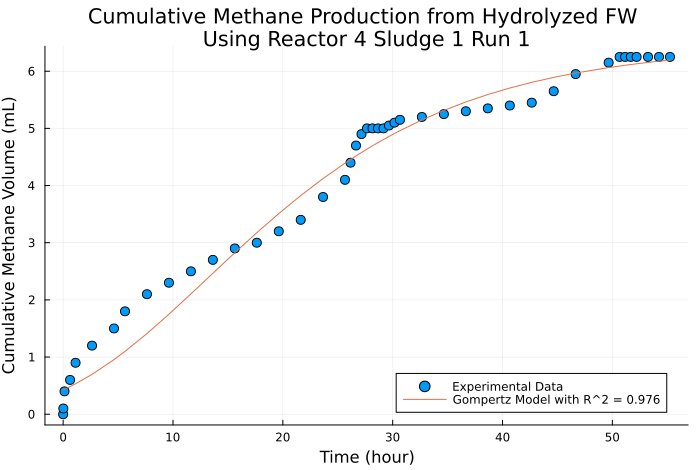
\includegraphics[width=.9\linewidth]{../plots/BMPs/Hydrolyzed FW/methane_kinetics_hydrolysate_4_s1_r1_hour.png}
\end{center}

\begin{center}
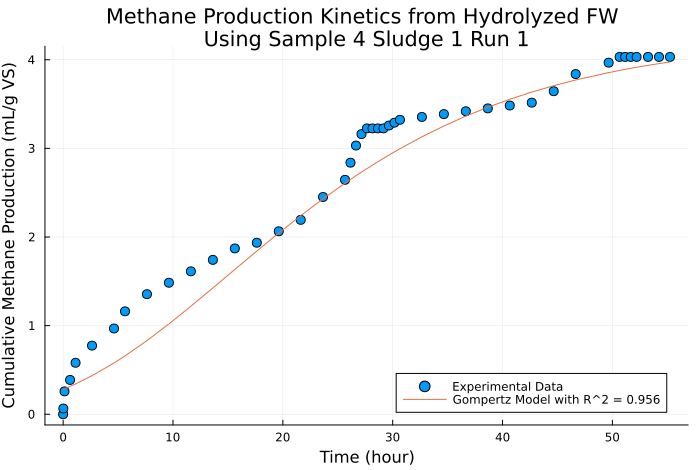
\includegraphics[width=.9\linewidth]{../plots/BMPs/Hydrolyzed FW/specific_methane_kinetics_hydrolysate_4_s1_r1_hour.png}
\end{center}

\subsection{Untreated FW}
\label{sec:org4cfbe9b}
Εκτός από τα παραπάνω, σε ένα από τα δοχεία προστέθηκε ανεπεξέργαστο FW. Αυτό έχει διαφορά από το δείγμα 0, καθώς εκείνο υπέστει ζύμωση κατά τις 72 ώρες που ήταν στους 40 \(^oC\) ακόμη και χωρίς να προσθέσουμε κάποιο εμβόλιο, ενώ το δείγμα αυτό αναφέρεται σε food waste το οποίο δεν έχει υποστεί καμία επεξεργασία. Θα θέλαμε το δείγμα αυτό να έχει το χειρότερο performance (είτε πολύ αργή παραγωγή, ή μικρή τελική παραγωγή), το οποίο θα μας επιδείκνυε πως η επεξεργασία που έγινε βοηθάει πραγματικά στην χώνευση. Βέβαια, αξίζει να αναφερθεί πως το δοχείο αυτό είχε κάποιο προβλήματα με διαρροή στα αρχικά στάδια του πειράματος, οπότε ενδέχεται τα αποτελέσματα που θα προκύψουν να μην είναι έγκυρα. Παρακάτω φαίνεται ο κώδικας επεξεργασίας των αποτελεσμάτων του.

\textbf{untreated\textsubscript{fw}\textsubscript{s1}\textsubscript{r1}}
\begin{minted}[breaklines=true,breakanywhere=true]{julia}

### Data Analysis on Untreated FW ###

<<date_saving_fw_s1_r1>>

inds = 22:71
exp_meth_vol = vcat([0, 0.05, 0, 0.1, 0.1, 0, 0, 0.1, 0.2, 0.1, 0, 0.1, 0.2, 0.1, 0.1, 0.1, 0.0, 0.1, 0.2, 0.1, 0.2, 0.1, 0.1], zeros(27))
meth_vol_hydro_fw = cumsum(exp_meth_vol)[end]
exp_name = "untreated_fw_s1_r1"
source = "Untreated FW"
reactor = "FW 1"
sludge = "Sludge 1"
run_num = "Run 1"

input_vs = 1.55

<<bmp_data_processing>>
max_rate_hydro_fw = max_manual_rate

p0 = [2.0, 0.001, 1.0]
<<bmp_curve_fitting_min>>
model_hydro_fw_min = vcat(reactor, round.(model_params, digits = 3), round(r_squared, digits = 3))
<<bmp_data_plotting>>

p0 = [2.0, 0.1, 0.1]
<<bmp_curve_fitting_hour>>
model_hydro_fw_hour = vcat(reactor, round.(model_params, digits = 3), round(r_squared, digits = 3))
<<bmp_data_plotting>>

<<sma_curve_fitting_hour>>
sma_hydro_fw = vcat(reactor, round.(model_params, digits = 3), round(r_squared, digits = 3))
<<bmp_data_plotting>>

return("../data/exp_pro/"*exp_name*".csv")
\end{minted}

\subsubsection{Results}
\label{sec:org3138415}
Το δείγμα αυτό παρήγαγε μόνο το \(7.1 \%\) του μεθανίου που είχε παράξει από οξικό και το έκανε αυτό σε έναν αργό σχετικά ρυθμό. Κρίνεται πιθανό να μην επιλύθηκαν τα προβλήματα διαρροής που είχε και η παραγωγή του αερίου να ήταν στην πραγματικότητα μεγαλύτερη. Όμως όπως και στο δείγμα με 0 ml ένζυμα το οποίο όμως υπέστει 3 μέρες υδρόλυση και ζύμωση, μας "βολεύει" τα ποσοστά αυτά να είναι πολύ χαμηλά επειδή σημαίνει πως η επεξεργασία που κάναμε όντως συνείσφερε στην παραγωγή μεθανίου.

Από άποψη προσαρμογής, το μοντέλο Gompertz μπορεί να προσαρμοστεί πολύ καλά σε τέτοια δεδομένα όπου η παραγωγή μεθανίου γίνεται σε παρόμοιο ρυθμό για όλη την διεργασία. Το μοντέλο που θα αντιστοιχήσει θα είναι ένα μοντέλο χαμηλού ρυθμού (με βάση την παραπάνω διάκριση), το οποίο όμως είναι το μόνο που μπορεί να ισχύει καθώς στην αρχή δεν υπάρχει μία απότομη παραγωγή αερίου ταχύτατα για να μπορεί να προσαρμοστεί κάτι διαφορετικό. Τα μοντέλα σε λεπτά και ώρες δεν προσαρμόζονται με τον ακριβώς ίδιο τρόπο, αλλά οι διαφορές τους είναι μικρές. Ο ειδικός ρυθμός ανάπτυξης είναι της τάξης του \(0.0137 \frac{ml}{g ~ sCOD \min} \text{ ή } 0.823 \frac{ml}{g ~ sCOD ~ hour}\). Τα άλλα μοντέλα που προσαρμόστηκαν με αργό ρυθμό ανάπτυξης είχαν κινητικές της τάξης του 0.03-0.05 \(\frac{ml}{g ~ sCOD \min }\) οπότε αυτό είναι πιο αργό αλλά συγκρίσιμο με εκείνα.

\begin{minted}[breaklines=true,breakanywhere=true]{elisp}
(org-table-import-after-n-lines 3 <<untreated_fw_s1_r1()>> '(4))
\end{minted}

\begin{center}
\begin{tabular}{lrrrr}
Timestamp & Minutes & Hours & Methane\textsubscript{Volume} & Cumulative\textsubscript{Methane}\textsubscript{Volume}\\[0pt]
02/04\textsubscript{10}:54 & 0.0 & 0.0 & 0.0 & 0.0\\[0pt]
02/04\textsubscript{12}:54 & 120.0074 & 2.0001 & 0.05 & 0.05\\[0pt]
02/04\textsubscript{13}:24 & 150.0073 & 2.5001 & 0.0 & 0.05\\[0pt]
02/04\textsubscript{13}:54 & 180.0076 & 3.0001 & 0.1 & 0.15\\[0pt]
02/04\textsubscript{14}:24 & 210.0076 & 3.5001 & 0.1 & 0.25\\[0pt]
02/04\textsubscript{14}:54 & 240.0075 & 4.0001 & 0.0 & 0.25\\[0pt]
02/04\textsubscript{15}:24 & 270.0074 & 4.5001 & 0.0 & 0.25\\[0pt]
02/04\textsubscript{15}:54 & 300.0073 & 5.0001 & 0.1 & 0.35\\[0pt]
02/04\textsubscript{16}:24 & 330.0076 & 5.5001 & 0.2 & 0.55\\[0pt]
02/04\textsubscript{16}:54 & 360.0076 & 6.0001 & 0.1 & 0.65\\[0pt]
02/04\textsubscript{17}:24 & 390.0073 & 6.5001 & 0.0 & 0.65\\[0pt]
02/04\textsubscript{17}:54 & 420.0141 & 7.0002 & 0.1 & 0.75\\[0pt]
02/04\textsubscript{19}:54 & 540.0146 & 9.0002 & 0.2 & 0.95\\[0pt]
02/04\textsubscript{21}:54 & 660.0162 & 11.0003 & 0.1 & 1.05\\[0pt]
02/04\textsubscript{23}:54 & 780.0205 & 13.0003 & 0.1 & 1.15\\[0pt]
03/04\textsubscript{01}:54 & 900.0205 & 15.0003 & 0.1 & 1.25\\[0pt]
03/04\textsubscript{03}:54 & 1020.0203 & 17.0003 & 0.0 & 1.25\\[0pt]
03/04\textsubscript{05}:54 & 1140.0253 & 19.0004 & 0.1 & 1.35\\[0pt]
03/04\textsubscript{07}:54 & 1260.0272 & 21.0005 & 0.2 & 1.55\\[0pt]
03/04\textsubscript{09}:54 & 1380.0273 & 23.0005 & 0.1 & 1.65\\[0pt]
03/04\textsubscript{12}:54 & 1560.0362 & 26.0006 & 0.2 & 1.85\\[0pt]
03/04\textsubscript{13}:54 & 1620.036 & 27.0006 & 0.1 & 1.95\\[0pt]
03/04\textsubscript{14}:24 & 1650.037 & 27.5006 & 0.1 & 2.05\\[0pt]
03/04\textsubscript{14}:54 & 1680.7956 & 28.0133 & 0.0 & 2.05\\[0pt]
03/04\textsubscript{15}:26 & 1712.8415 & 28.5474 & 0.0 & 2.05\\[0pt]
03/04\textsubscript{16}:29 & 1775.1124 & 29.5852 & 0.0 & 2.05\\[0pt]
03/04\textsubscript{17}:29 & 1835.1168 & 30.5853 & 0.0 & 2.05\\[0pt]
03/04\textsubscript{18}:29 & 1895.1168 & 31.5853 & 0.0 & 2.05\\[0pt]
03/04\textsubscript{20}:29 & 2015.1168 & 33.5853 & 0.0 & 2.05\\[0pt]
03/04\textsubscript{21}:29 & 2075.117 & 34.5853 & 0.0 & 2.05\\[0pt]
03/04\textsubscript{22}:29 & 2135.1168 & 35.5853 & 0.0 & 2.05\\[0pt]
03/04\textsubscript{23}:29 & 2195.1234 & 36.5854 & 0.0 & 2.05\\[0pt]
04/04\textsubscript{00}:29 & 2255.1235 & 37.5854 & 0.0 & 2.05\\[0pt]
04/04\textsubscript{01}:29 & 2315.1236 & 38.5854 & 0.0 & 2.05\\[0pt]
04/04\textsubscript{02}:29 & 2375.1236 & 39.5854 & 0.0 & 2.05\\[0pt]
04/04\textsubscript{03}:29 & 2435.1237 & 40.5854 & 0.0 & 2.05\\[0pt]
04/04\textsubscript{04}:29 & 2495.1236 & 41.5854 & 0.0 & 2.05\\[0pt]
04/04\textsubscript{05}:29 & 2555.1238 & 42.5854 & 0.0 & 2.05\\[0pt]
04/04\textsubscript{06}:29 & 2615.1235 & 43.5854 & 0.0 & 2.05\\[0pt]
04/04\textsubscript{07}:29 & 2675.1235 & 44.5854 & 0.0 & 2.05\\[0pt]
04/04\textsubscript{08}:29 & 2735.1276 & 45.5855 & 0.0 & 2.05\\[0pt]
04/04\textsubscript{09}:29 & 2795.1321 & 46.5855 & 0.0 & 2.05\\[0pt]
04/04\textsubscript{10}:29 & 2855.1336 & 47.5856 & 0.0 & 2.05\\[0pt]
04/04\textsubscript{11}:29 & 2915.1339 & 48.5856 & 0.0 & 2.05\\[0pt]
04/04\textsubscript{12}:29 & 2975.134 & 49.5856 & 0.0 & 2.05\\[0pt]
04/04\textsubscript{13}:29 & 3035.134 & 50.5856 & 0.0 & 2.05\\[0pt]
04/04\textsubscript{14}:29 & 3095.1341 & 51.5856 & 0.0 & 2.05\\[0pt]
04/04\textsubscript{15}:29 & 3155.1342 & 52.5856 & 0.0 & 2.05\\[0pt]
04/04\textsubscript{16}:29 & 3215.134 & 53.5856 & 0.0 & 2.05\\[0pt]
04/04\textsubscript{17}:29 & 3275.1482 & 54.5858 & 0.0 & 2.05\\[0pt]
\end{tabular}
\end{center}

\begin{center}
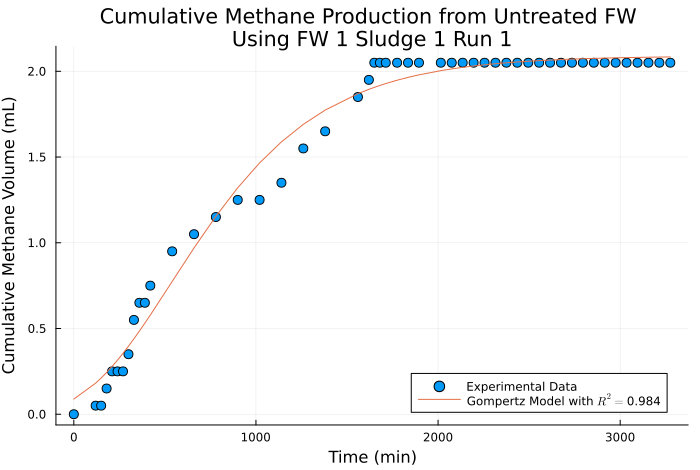
\includegraphics[width=.9\linewidth]{../plots/BMPs/Untreated FW/methane_kinetics_untreated_fw_s1_r1_min.png}
\end{center}

\begin{center}
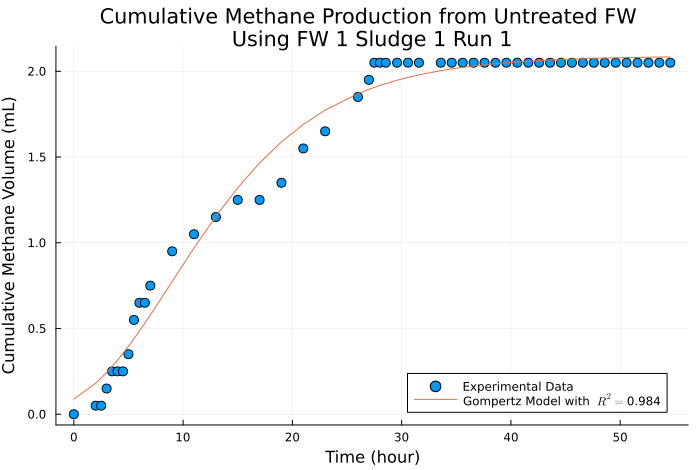
\includegraphics[width=.9\linewidth]{../plots/BMPs/Untreated FW/methane_kinetics_untreated_fw_s1_r1_hour.png}
\end{center}

\begin{center}
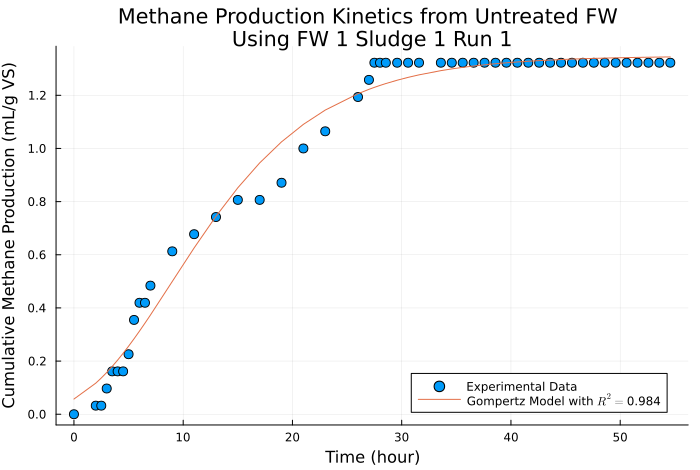
\includegraphics[width=.9\linewidth]{../plots/BMPs/Untreated FW/specific_methane_kinetics_untreated_fw_s1_r1_hour.png}
\end{center}

\subsection{Update all}
\label{sec:org09b6514}

\textbf{update\textsubscript{hydrolysate}\textsubscript{tests}\textsubscript{s1}\textsubscript{r1}}
\begin{minted}[breaklines=true,breakanywhere=true]{julia}

<<hydrolysate_0_s1_r1>>
<<hydrolysate_1_s1_r1>>
<<hydrolysate_2_s1_r1>>
<<hydrolysate_4_s1_r1>>
<<untreated_fw_s1_r1>>

model_fit_table_min = Tables.table(vcat(reshape(model_hydro_0_min, 1, 5), reshape(model_hydro_1_min, 1, 5), reshape(model_hydro_2_min, 1, 5), reshape(model_hydro_4_min, 1, 5), reshape(model_hydro_fw_min, 1, 5)), header = [:Reactor_Name, :Production_Potential, :Production_Rate, :Lag_Time, :R_squared])
CSV.write(datadir("exp_pro", "methane_from_hydrolysate_kinetics_min_s1_r1.csv"), model_fit_table_min)

model_fit_table_hour = Tables.table(vcat(reshape(model_hydro_0_hour, 1, 5), reshape(model_hydro_1_hour, 1, 5), reshape(model_hydro_2_hour, 1, 5), reshape(model_hydro_4_hour, 1, 5), reshape(model_hydro_fw_hour, 1, 5)), header = [:Reactor_Name, :Production_Potential, :Production_Rate, :Lag_Time, :R_squared])
CSV.write(datadir("exp_pro", "methane_from_hydrolysate_kinetics_hour_s1_r1.csv"), model_fit_table_hour)
return("../data/exp_pro/methane_from_hydrolysate_kinetics_min_s1_r1.csv")
\end{minted}

\begin{minted}[breaklines=true,breakanywhere=true]{julia}

return("../data/exp_pro/methane_from_hydrolysate_kinetics_hour_s1_r1.csv")
\end{minted}

\begin{minted}[breaklines=true,breakanywhere=true]{elisp}
(org-table-import-after-n-lines 4 <<hydrolysate_kinetic_name_hour_s1_r1()>> '(4))
\end{minted}

\begin{table}[htbp]
\caption{Kinetics with timescale in hours}
\centering
\begin{tabular}{lrrrr}
Reactor\textsubscript{Name} & Production\textsubscript{Potential} & Production\textsubscript{Rate} & Lag\textsubscript{Time} & R\textsubscript{squared}\\[0pt]
Reactor 0 & 5.56 & 0.094 & 5.994 & 0.992\\[0pt]
Reactor 1 & 11.309 & 0.264 & 3.652 & 0.979\\[0pt]
Reactor 2 & 7.182 & 0.187 & 1.108 & 0.991\\[0pt]
Reactor 4 & 5.902 & 0.17 & 1.948 & 0.988\\[0pt]
FW 1 & 2.09 & 0.099 & 1.174 & 0.984\\[0pt]
\end{tabular}
\end{table}

\begin{minted}[breaklines=true,breakanywhere=true]{elisp}
(org-table-import-after-n-lines 4 <<update_hydrolysate_tests_s1_r1()>> '(4))
\end{minted}

\begin{table}[htbp]
\caption{Kinetics with timescale in minutes}
\centering
\begin{tabular}{lrrrr}
Reactor\textsubscript{Name} & Production\textsubscript{Potential} & Production\textsubscript{Rate} & Lag\textsubscript{Time} & R\textsubscript{squared}\\[0pt]
Reactor 0 & 5.56 & 0.002 & 359.624 & 0.992\\[0pt]
Reactor 1 & 11.309 & 0.004 & 219.136 & 0.979\\[0pt]
Reactor 2 & 7.182 & 0.003 & 66.5 & 0.991\\[0pt]
Reactor 4 & 5.902 & 0.003 & 116.91 & 0.988\\[0pt]
FW 1 & 2.09 & 0.002 & 70.446 & 0.984\\[0pt]
\end{tabular}
\end{table}

\begin{minted}[breaklines=true,breakanywhere=true]{julia}

<<hydrolysate_0_s1_r1>>
<<hydrolysate_1_s1_r1>>
<<hydrolysate_2_s1_r1>>
<<hydrolysate_4_s1_r1>>
<<untreated_fw_s1_r1>>

sma_table = Tables.table(vcat(reshape(sma_hydro_0, 1, 5), reshape(sma_hydro_1, 1, 5), reshape(sma_hydro_2, 1, 5), reshape(sma_hydro_4, 1, 5), reshape(sma_hydro_fw, 1, 5)), header = [:Reactor_Name, :Methane_Potential, :SMA, :Lag_Time, :R_sq])
CSV.write(datadir("exp_pro", "sma_from_hydrolysate_s1_r1.csv"), sma_table)

return("../data/exp_pro/sma_from_hydrolysate_s1_r1.csv")
\end{minted}

\begin{minted}[breaklines=true,breakanywhere=true]{elisp}
(org-table-import-after-n-lines 4 <<sma_hydro_s1_r1()>> '(4))
\end{minted}

\begin{table}[htbp]
\caption{SMA Kinetics in hours}
\centering
\begin{tabular}{lrrrr}
Reactor\textsubscript{Name} & Methane\textsubscript{Potential} & SMA & Lag\textsubscript{Time} & R\textsubscript{sq}\\[0pt]
Reactor 0 & 3.587 & 0.061 & 5.994 & 0.992\\[0pt]
Reactor 1 & 7.296 & 0.17 & 3.652 & 0.979\\[0pt]
Reactor 2 & 4.633 & 0.121 & 1.108 & 0.991\\[0pt]
Reactor 4 & 3.808 & 0.11 & 1.948 & 0.988\\[0pt]
FW 1 & 1.348 & 0.064 & 1.174 & 0.984\\[0pt]
\end{tabular}
\end{table}

\subsection{Plotting Methane Potential}
\label{sec:org9a69fc2}
Σε αυτό το section θα γίνει ένα plot το οποίο θα συγκρίνει μέγιστο μεθάνιο (παραγωγή από οξικό) με αυτό που παράχθηκε από το FW. Το plotting θα γίνει μέσω του \texttt{CairoMakie.jl} το οποίο είναι αρκετά featureful. Η διαδικασία είναι πως βάζουμε όλους τους όγκους παραγόμενου μεθανίου σε ένα vector και εκτός από την απόλυτη τιμή, υπολογίζουμε και το ποσοστό του μέγιστου που πετυχαίνει το υδρόλυμα. Όπως έχουν αποθηκευτεί, αυτό είναι διαίρεση του στοιχείου i+5 με το i. Έπειτα φτιάχνουμε ένα string των ποσοστών αυτών μαζί με τα labels που τους αντιστοιχούν. Αυτό θα προστεθεί στο plot που φτιάχνουμε.

Έχοντας κάνει το preprocessing αυτό, ξεκινάμε την δημιουργία διαγραμμάτων. Φτιάχνουμε ένα figure και έναν άξονα πάνω σε αυτό όπου θα κάνουμε τα bar plots που θέλουμε. Οι μεταβλητές \texttt{xdata} και \texttt{grp} είναι απαραίτητες για να φτιαχτεί το plot. Το xdata λέει σε ποιό σημείο του άξονα x θα πάει κάθε δεδομένο (όπως τα έχουμε ορίσει θα είναι από το 1 εώς το 5 δύο φορές) ενώ το grp λέει σε ποιό group θα ανήκει το κάθε πείραμα. Τα 5 πρώτα είναι στο group 1 (οξικό) ενώ τα άλλα στο 2 (υδρόλυμα). Ορίζουμε και το legend και το plot αυτό είναι έτοιμο. Από κάτω, κάνουμε insert το string με τα ποσοστά που υπολογίστηκε παραπάνω σε ένα text plot του Makie. Έπειτα, κάνουμε save το plot αυτό.

\textbf{BMP\textsubscript{comp}\textsubscript{plot}}
\begin{minted}[breaklines=true,breakanywhere=true]{julia}

using CairoMakie
colors = Makie.wong_colors()

meth_vol = [meth_vol_acet_0, meth_vol_acet_1, meth_vol_acet_2, meth_vol_acet_4, meth_vol_acet_fw, meth_vol_hydro_0, meth_vol_hydro_1, meth_vol_hydro_2, meth_vol_hydro_4, meth_vol_hydro_fw]

percent_bmp = [meth_vol[i+5]/meth_vol[i] for i in 1:5]
string_bmp = vcat(string.(round.(percent_bmp.*100, digits = 2)).*" %", ["0 ml", "1 ml", "2 ml", "4 ml", "Untreated \nFW"])

fig = Figure(size = (600, 400))
ax = Axis(fig[1,1], xticks = (1:5, ["0 ml", "1 ml", "2 ml", "4 ml", "Untreated FW"]),
          title = "Acetate vs Hydrolysate BMP - "*sludge*run, ylabel = "Methane Produced (ml)")

xdata = [1, 2, 3, 4, 5, 1, 2, 3, 4, 5]
grp = [1, 1, 1, 1, 1, 2, 2, 2, 2, 2]

barplot!(ax, xdata, meth_vol,
        dodge = grp,
        color = colors[grp])

# Legend
labels = ["Acetate", "FW Hydrolysate"]
elements = [PolyElement(polycolor = colors[i]) for i in 1:length(labels)]
title = "Source"
Legend(fig[1,2], elements, labels, title)

ax2 = Axis(fig[2, 1], xticks = (1:5, ["0 ml", "1 ml", "2 ml", "4 ml", "Untreated FW"]), yticks = ([1, 2], ["", ""]), title = "% of Acetate BMP in Hydrolysates")
hidespines!(ax2)
hidedecorations!(ax2)
text!(xdata, repeat(1:1, 10), text = string_bmp, align = [(:left, :top), (:left, :top), (:center, :top), (:right, :top), (:right, :top), (:left, :bottom), (:left, :bottom), (:center, :bottom), (:right, :bottom), (:right, :bottom)])

save(plotsdir("BMPs", "Hydrolyzed FW", "acet_vs_hydro_bmp_"*comp_name*".png"), fig)
\end{minted}

Για να τρέξουμε αυτό το code block χωρίς προβλήματα, πρέπει να δώσουμε τιμή στο \texttt{comp\_name} και να κάνουμε update τα tests ώστε να έχουμε τα σωστά.
\begin{minted}[breaklines=true,breakanywhere=true]{julia}

<<update_acetate_tests_s1>>
<<update_hydrolysate_tests_s1_r1>>

comp_name = "s1_r1"
sludge = "Sludge 1 "
run = "Run 1"
<<BMP_comp_plot>>
\end{minted}

\begin{center}
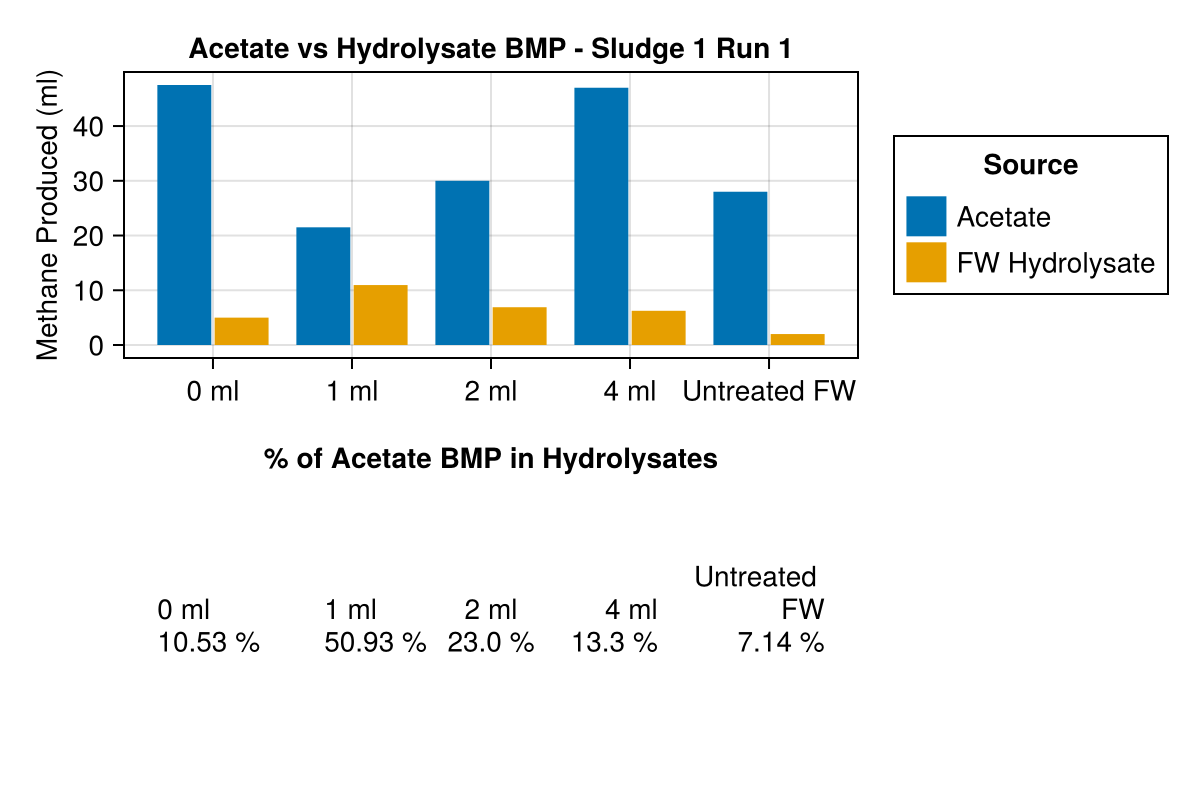
\includegraphics[width=.9\linewidth]{../plots/BMPs/Hydrolyzed FW/acet_vs_hydro_bmp_s1_r1.png}
\end{center}

\subsection{Comparing Kinetic Constants}
\label{sec:org8e93214}
Έχοντας συγκρίνει το μέγιστο παραγώμενο βιομεθάνιο μεταξύ οξικού και των υδρολυμάτων, αξίζει να συγκρίνουμε και τους ρυθμούς παραγωγής μεθανίου σε κάθε περίπτωση για να δούμε ποιό πείραμα είναι το καλύτερο. Πάλι δεν θα συγκρίνουμε τους ρυθμούς μεταξύ τους, αλλά θα τους συγκρίνουμε με βάση το οξικό τους. Επειδή αρκετά έχουν διαφορετικές μονάδες, θα κάνουμε read τα CSVs τους και θα κάνουμε τα απαραίτητα conversions. Για το πείραμα αυτό που υπάρχουν δυο ρυθμοί, θα πάρουμε τον αργό ρυθμό, καθώς ο γρήγορος είναι μάλλον έντονα επηρεασμένος από το οξικό. 

\begin{minted}[breaklines=true,breakanywhere=true]{julia}

acet_kinetics = CSV.read(datadir("exp_pro", "methane_from_acetate_kinetics_"*sludge*".csv"), DataFrame)
hydro_kinetics = CSV.read(datadir("exp_pro", "methane_from_hydrolysate_kinetics_"*timescale*"_"*sludge*"_"*run_num*".csv"), DataFrame)

# Acetate rates are in minutes while hydrolysate in hours
acet_rates = acet_kinetics.Production_Rate
hydro_rates = hydro_kinetics.Production_Rate

# Convert Acetate rates to hours
acet_rates_hour = acet_rates.*60

# Find what percentage of acetate each hydrolysate is
acet_percent_hydro = round.((hydro_rates./acet_rates_hour).*100, digits = 4)

# Create a new table with the 2 rates and their ratio
kinetic_comp = Tables.table(hcat(acet_kinetics.Reactor_Name, acet_rates_hour, hydro_rates, acet_percent_hydro), header = [:Reactor_Name, :Acetate, :Hydrolysate, :Ratio])
CSV.write(datadir("exp_pro", "kinetics_comparison_"*sludge*"_"*run_num*".csv"), kinetic_comp)

# We can also do this for SMA
acet_sma_kinetics = CSV.read(datadir("exp_pro", "sma_from_acetate_"*sludge*".csv"), DataFrame)
hydro_sma_kinetics = CSV.read(datadir("exp_pro", "sma_from_hydrolysate_"*sludge*"_"*run_num*".csv"), DataFrame)

# Acetate rates are in minutes while hydrolysate in hours
acet_sma = acet_sma_kinetics.SMA
hydro_sma = hydro_sma_kinetics.SMA

# SMA is commonly expressed per day so convert to days
acet_sma_day = round.(acet_sma.*(60*24), digits = 3)
hydro_sma_day = round.(hydro_sma.*24, digits = 3)

# Find what percentage of acetate each hydrolysate is
acet_percent_hydro_sma = round.((hydro_sma_day./acet_sma_day).*100, digits = 4)

# Create a new table with the 2 rates and their ratio
sma_comp = Tables.table(hcat(acet_sma_kinetics.Reactor_Name, acet_sma_day, hydro_sma_day, acet_percent_hydro_sma), header = [:Reactor_Name, :Acetate, :Hydrolysate, :Ratio])
CSV.write(datadir("exp_pro", "kinetics_comparison_sma_"*sludge*"_"*run_num*".csv"), sma_comp)

\end{minted}

\begin{minted}[breaklines=true,breakanywhere=true]{julia}

<<update_acetate_tests_s1>>
<<update_hydrolysate_tests_s1_r1>>

sludge = "s1"
run = "r1"
timescale = "hour"

<<ad_kinetics_comparison>>
return("../data/exp_pro/kinetics_comparison_s1_r1.csv")
\end{minted}

\begin{minted}[breaklines=true,breakanywhere=true]{julia}
return("../data/exp_pro/kinetics_comparison_sma_s1_r1.csv")
\end{minted}

Εκτός από αυτή την σύγκριση, θα κάνουμε και μία σύγκριση ρυθμών βασιζόμενοι στον "μέγιστο" στιγμιαίο ρυθμό παραγωγής που υπολογίζεται αλγεβρικά και όχι με χρήση μοντέλου. Αυτοί οι ρυθμοί έχουν γίνουν eval'd για κάθε μοντέλο οπότε μπορούν να γίνουν exported εδώ για περαιτέρω χρήση.

\begin{minted}[breaklines=true,breakanywhere=true]{julia}

reactors = ["Reactor 0", "Reactor 1", "Reactor 2", "Reactor 4", "Reactor FW"]
max_rate_acet = round.(vcat(max_rate_acet_0, max_rate_acet_1, max_rate_acet_2, max_rate_acet_4, max_rate_acet_fw), digits = 3)
max_rate_hydro = round.(vcat(max_rate_hydro_0, max_rate_hydro_1, max_rate_hydro_2, max_rate_hydro_4, max_rate_hydro_fw), digits = 3)

ratio = round.((max_rate_hydro./max_rate_acet)*100, digits = 3)

max_rate_comp = Tables.table(hcat(reactors, max_rate_acet, max_rate_hydro, ratio), header = [:Reactor, :Acetate, :Hydrolysate, :Ratio])
CSV.write(datadir("exp_pro", "manual_max_rate_comp_"*sludge*"_"*run*".csv"), max_rate_comp)
\end{minted}

\begin{minted}[breaklines=true,breakanywhere=true]{julia}

<<update_acetate_tests_s1>>
<<update_hydrolysate_tests_s1_r1>>

sludge = "s1"
run = "r1"

<<manual_rate_comparison>>
return("../data/exp_pro/manual_max_rate_comp_s1_r1.csv")
\end{minted}

\begin{minted}[breaklines=true,breakanywhere=true]{elisp}
(org-table-import-after-n-lines 4 <<kinetics_comp_s1_r1()>> '(4))
\end{minted}

\begin{table}[htbp]
\caption{Kinetic Comparison with timescale in hours}
\centering
\begin{tabular}{lrrr}
Reactor\textsubscript{Name} & Acetate & Hydrolysate & Ratio\\[0pt]
Reactor 0 & 459.84 & 0.148 & 0.0322\\[0pt]
Reactor 1 & 326.88 & 0.29 & 0.0887\\[0pt]
Reactor 2 & 374.04 & 0.187 & 0.05\\[0pt]
Reactor 4 & 579.0 & 0.181 & 0.0313\\[0pt]
Reactor FW & 294.06 & 0.081 & 0.0275\\[0pt]
\end{tabular}
\end{table}

\begin{minted}[breaklines=true,breakanywhere=true]{elisp}
(org-table-import-after-n-lines 4 <<sma_comp_s1_r1()>> '(4))
\end{minted}

\begin{table}[htbp]
\caption{SMA Comparison with timescale in days}
\centering
\begin{tabular}{lrrr}
Reactor\textsubscript{Name} & Acetate & Hydrolysate & Ratio\\[0pt]
Reactor 0 & 7119.36 & 2.304 & 0.0324\\[0pt]
Reactor 1 & 5061.6 & 3.912 & 0.0773\\[0pt]
Reactor 2 & 5676.48 & 2.808 & 0.0495\\[0pt]
Reactor 4 & 8965.44 & 2.52 & 0.0281\\[0pt]
Reactor FW & 4554.72 & 1.248 & 0.0274\\[0pt]
\end{tabular}
\end{table}

\begin{minted}[breaklines=true,breakanywhere=true]{elisp}
(org-table-import-after-n-lines 3 <<manual_rates_s1_r1()>> '(4))
\end{minted}

\begin{table}[htbp]
\caption{Max Rate Manually with timescale in hours}
\centering
\begin{tabular}{lrrr}
Reactor & Acetate & Hydrolysate & Ratio\\[0pt]
Reactor 0 & 1025.641 & 11.976 & 1.168\\[0pt]
Reactor 1 & 643.564 & 36.232 & 5.63\\[0pt]
Reactor 2 & 555.556 & 0.989 & 0.178\\[0pt]
Reactor 4 & 1081.081 & 5.988 & 0.554\\[0pt]
Reactor FW & 705.882 & 0.2 & 0.028\\[0pt]
\end{tabular}
\end{table}

\subsection{Plotting Comparison Plots}
\label{sec:org60f93b8}
Εκτός από τα παραπάνω, ένα χρήσιμο διάγραμμα θα ήταν να φαίνονται στο ίδιο figure και τα 5 πειράματα με τα υδρολύματα, το οποίο είναι πολύ χρήσιμο για μία όπτικη σύγκριση τους. Καθώς δεν κάνουμε save όλα τα απαραίτητα στοιχεία, το plot θα φτιαχτεί step wise κάνοντας update κάθε καμπύλη.

\begin{minted}[breaklines=true,breakanywhere=true]{julia}

colors = ["#009AFA","#E36F47","#3EA44E","#C371D2","#AC8E18"]

<<hydrolysate_0_s1_r1>>
methane_s1_r1_comp = scatter(exp_hour, cumsum(exp_meth_vol), markersize = 4, legend = :outerright, label = "Hydrolysate (0 ml mix) Exp", xlabel = "Time (hour)", ylabel = "Cumulative Methane Volume (mL)", markercolor = colors[1], size = (1000, 600), legendfontsize = 12, labelfontsize = 14, tickfontsize = 12, left_margin=3Plots.mm,  bottom_margin=3Plots.mm)
plot!(exp_hour, gompertz_bmp(exp_hour, model_hydro_0_hour[2:4]), label = "Hydrolysate (0 ml mix) Theoretical\n with "*L"R^2 = "*string(model_hydro_0_hour[5]), linecolor = colors[1])

<<hydrolysate_1_s1_r1>>
scatter!(methane_s1_r1_comp, exp_hour, cumsum(exp_meth_vol), markersize = 4, label = "Hydrolysate (1 ml mix) Exp", markercolor = colors[2])
plot!(exp_hour, gompertz_bmp(exp_hour, model_hydro_1_hour[2:4]), label = "Hydrolysate (1 ml mix) Theoretical\n with "*L"R^2 = "*string(model_hydro_1_hour[5]), linecolor = colors[2])

<<hydrolysate_2_s1_r1>>
scatter!(methane_s1_r1_comp, exp_hour, cumsum(exp_meth_vol), markersize = 4, label = "Hydrolysate (2 ml mix) Exp", markercolor = colors[3])
plot!(exp_hour, gompertz_bmp(exp_hour, model_hydro_2_hour[2:4]), label = "Hydrolysate (2 ml mix) Theoretical\n with "*L"R^2 = "*string(model_hydro_2_hour[5]), linecolor = colors[3])

<<hydrolysate_4_s1_r1>>
scatter!(methane_s1_r1_comp, exp_hour, cumsum(exp_meth_vol), markersize = 4, label = "Hydrolysate (4 ml mix) Exp", markercolor = colors[4])
plot!(exp_hour, gompertz_bmp(exp_hour, model_hydro_4_hour[2:4]), label = "Hydrolysate (4 ml mix) Theoretical\n with "*L"R^2 = "*string(model_hydro_4_hour[5]), linecolor = colors[4])

<<untreated_fw_s1_r1>>
scatter!(methane_s1_r1_comp, exp_hour, cumsum(exp_meth_vol), markersize = 4, label = "Untreated FW Exp", markercolor = colors[5])
plot!(exp_hour, gompertz_bmp(exp_hour, model_hydro_fw_hour[2:4]), label = "Untreated FW Theoretical\n with "*L"R^2 = "*string(model_hydro_fw_hour[5]), linecolor = colors[5])

savefig(methane_s1_r1_comp, plotsdir("BMPs", "methane_s1_r1_comp.svg"))
\end{minted}

\begin{center}
\includesvg[width=.9\linewidth]{../plots/BMPs/methane_s1_r1_comp}
\end{center}

\subsection{Συμπεράσματα του πειραματικού κύκλου αυτού}
\label{sec:orgc8b49d1}
Το πείραμα αυτό ήταν το πρώτο πείραμα όπου τροφοδοτήσαμε με υδρολύματα από FW για να δούμε την απόκριση του συστήματος σε αυτά.

Ο κύκλος αυτός είχε κάποια προβλήματα στην ανάλυση δεδομένων, αλλά μετά από κάποια επεξεργασία, ήρθαν σε μία μορφή η οποία βγάζει νόημα και είναι συγκρίσιμη με την άλλη επανάληψη, η οποία φαίνεται παρακάτω.

Μία περίεργη παρατήρηση η οποία σίγουρα αξίζει να σημειωθεί είναι πως κανένα από τα μοντέλα δεν είχε lag time. Αυτό είχε παρατηρηθεί και στα πειράματα με το οξικό. Γενικά, το lag time είναι μία φυσική παράμετρος του συστήματος που εκφράζει πόσο γρήγορα αντιδρά το σύστημα με μία αλλαγή στο περιβάλλον του. Για την προσθήκη οξικού είναι λογικό το μηδενικό lag time καθώς είναι το ιδανικό υπόστρωμα του συστήματος. Για το υδρόλυμα, θα αναμενόταν πιθανόν κάποιο lag time, αλλά στο πείραμα αυτό δεν παρατηρήθηκε κάτι τέτοιο.

Ως προς το biomethane potential (BMP) του συστήματος, όπως θα αναμενόταν τα υδρολύματα παρήγαγαν λιγότερο μεθάνιο από το οξικό. Για την σύγκριση των πειράματων, έγινε έμμεσα συγκρίνοντας τι ποσοστό του αντίστοιχου οξικού ήταν το καθένα. Η χαμηλότερη παραγωγικότητα ήταν από το FW, το οποίο είναι καλό συμπέρασμα επειδή δείχνει την σημασία της προεπεξεργασίας. Υπήρχε μία υπόθεση ότι μπορεί να διέρρεε αέριο από το δοχείο αυτό, αλλά εν τέλει, με βάση τα πειράματα του 2ου κύκλου, έγινε overacidification το οποίο οδήγησε σε κατάρρευση του συστήματος.

Λόγω των προβλημάτων που παρουσιάστηκαν και για να επιβεβαιώσουμε αν είναι επαναλήψιμα αυτά, έγινε και ένα δεύτερο πείραμα με τις ίδιες συνθήκες για να δούμε τα αποτελέσματα του.

\subsection{Code Block για Tangling}
\label{sec:orgfb96950}
Έχοντας κάνει όλη αυτήν την ανάλυση, κάνουμε tangle ένα συνολικό code block σε ένα julia script file για sharing. Λόγω του structure του αρχείου αυτού και το ότι βασίζεται αρκετά στο org babel και το noweb syntax, το script file θα έχει αναγκαστικά πολλές επαναλήψεις. Αλλά θα είναι perfectly usable σε άλλο υπολογιστή θεωρητικά.

\begin{minted}[breaklines=true,breakanywhere=true]{julia}

<<update_acetate_tests_s1>>

sma_table = Tables.table(vcat(reshape(sma_acet_0, 1, 5), reshape(sma_acet_1, 1, 5), reshape(sma_acet_2, 1, 5), reshape(sma_acet_4, 1, 5), reshape(sma_acet_fw, 1, 5)), header = [:Reactor_Name, :Methane_Potential, :SMA, :Lag_Time, :R_sq])
CSV.write(datadir("exp_pro", "sma_from_acetate_s1.csv"), sma_table)

<<update_hydrolysate_tests_s1_r1>>

sma_table = Tables.table(vcat(reshape(sma_hydro_0, 1, 5), reshape(sma_hydro_1, 1, 5), reshape(sma_hydro_2, 1, 5), reshape(sma_hydro_4, 1, 5), reshape(sma_hydro_fw, 1, 5)), header = [:Reactor_Name, :Methane_Potential, :SMA, :Lag_Time, :R_sq])
CSV.write(datadir("exp_pro", "sma_from_hydrolysate_s1_r1.csv"), sma_table)

comp_name = "s1_r1"
sludge = "Sludge 1 "
run = "Run 1"
<<BMP_comp_plot>>

sludge = "s1"
run = "r1"
timescale = "hour"

<<ad_kinetics_comparison>>
<<manual_rate_comparison>>
\end{minted}

\section{FW Hydrolysate S1\textsubscript{R2} Processing}
\label{sec:orgfa2cf8e}
Στο section αυτό θα αναλυθούν τα αποτελεσματα του δεύτερου πειράματος που χρησιμοποιήσε FW hydrolysate ως υπόστρωμα (S1\textsubscript{R2} επειδή είναι το δεύτερο run με την πρώτη λάσπη). Βρίσκεται σε πλήρη αντιστοιχία με το προηγούμενο πείραμα και έγινε για επαναληψιμότητα. Οπότε, σκοπός είναι να εξετάσουμε αν είναι παρόμοιο με το προηγούμενο ή αν διαφέρει σημαντικά και στην περίπτωση του 2ου, να κρίνουμε ποιά από τις δύο περιπτώσεις είναι πραγματικά ο outlier. Τα σχόλια για το τι είναι κάθε δείγμα θα μείνουν ίδια με παραπάνω για υπενθύμιση.

\subsection{Reactor 0}
\label{sec:org93e1d3e}
Το δείγμα αυτό είναι labelled ως δείγμα 0 καθώς είναι το δείγμα το οποίο τροφοδοτήθηκε με treated FW, όμως χωρίς προσθήκη του μιξ ενζύμων και μικροοργανισμών. Όπως έχουμε δεί, όλες οι αντιδράσεις που γίνονται κατά την υδρόλυση και ζύμωση μπορούν να γίνουν και χωρίς το μιξ. Όμως, γινόντουσαν πιο αποτελεσματικά με την προσθήκη αυτού. Οπότε, ελπίζουμε πως το δείγμα αυτό θα έχει χειρότερα αποτελέσματα από τα άλλα, το οποίο θα μας οδηγήσει στην υπόθεση ότι το μιξ βελτιώνει όχι μόνο τα κριτήρια υδρόλυσης και οξεογένεσης αλλά και αυτό της μεθανογένεσης.

\textbf{hydrolysate\textsubscript{0}\textsubscript{s1}\textsubscript{r2}}
\begin{minted}[breaklines=true,breakanywhere=true]{julia}

### Data Analysis on Hydrolysate with 0 ml ###

<<date_saving_fw_s1_r2>>

inds = 1:73
exp_meth_vol = [0, 0, 0, 0, 0, 0, 0, 0.1, 0.1, 0.1, 0.05, 0.1, 0.1, 0.05, 0.1, 0.1, 0.1, 0.1, 0.1, 0.05, 0.1, 0.1, 0.1, 0.1, 0.1, 0.1, 0, 0, 0, 0, 0, 0, 0, 0, 0.1, 0.1, 0.1, 0.1, 0.05, 0.05, 0.1, 0.05, 0, 0, 0.05, 0.05, 0.05, 0.1, 0.05, 0.05, 0.05, 0.05, 0.1, 0.1, 0.1, 0.05, 0.05, 0.05, 0.05, 0, 0.05, 0, 0.02, 0.02, 0.01, 0, 0, 0, 0, 0, 0, 0, 0]
meth_vol_hydro_0 = cumsum(exp_meth_vol)[end]

exp_name = "hydrolysate_0_s1_r2"
source = "Hydrolyzed FW"
reactor = "Reactor 0"
sludge = "Sludge 1"
run_num = "Run 2"
input_vs = 1.55

<<bmp_data_processing>>
max_rate_hydro_0 = max_manual_rate

# The same model is fit either with min or hour
p0 = [5.0, 0.04, 1.0]
<<bmp_curve_fitting_min>>
model_hydro_0_min = vcat(reactor, round.(model_params, digits = 4), round(r_squared, digits = 3))
<<bmp_data_plotting>>

p0 = [4.0, 0.1, 1.0]
<<bmp_curve_fitting_hour>>
model_hydro_0_hour = vcat(reactor, round.(model_params, digits = 3), round(r_squared, digits = 3))
<<bmp_data_plotting>>

<<sma_curve_fitting_hour>>
sma_hydro_0 = vcat(reactor, round.(model_params, digits = 3), round(r_squared, digits = 3))
<<bmp_data_plotting>>

return("../data/exp_pro/"*exp_name*".csv")
\end{minted}

\subsubsection{Results}
\label{sec:orgf7bc494}
Παρακάτω φαίνονται τα αποτελέσματα του σχετικού πειράματος.

\begin{minted}[breaklines=true,breakanywhere=true]{elisp}
(org-table-import-after-n-lines 3 <<hydrolysate_0_s1_r2()>> '(4))
\end{minted}

\begin{center}
\begin{tabular}{lrrrr}
Timestamp & Minutes & Hours & Methane\textsubscript{Volume} & Cumulative\textsubscript{Methane}\textsubscript{Volume}\\[0pt]
03/04\textsubscript{14}:37 & 0.0 & 0.0 & 0.0 & 0.0\\[0pt]
03/04\textsubscript{14}:45 & 8.4249 & 0.1404 & 0.0 & 0.0\\[0pt]
03/04\textsubscript{14}:51 & 14.5619 & 0.2427 & 0.0 & 0.0\\[0pt]
03/04\textsubscript{14}:56 & 19.6074 & 0.3268 & 0.0 & 0.0\\[0pt]
03/04\textsubscript{15}:29 & 51.8783 & 0.8646 & 0.0 & 0.0\\[0pt]
03/04\textsubscript{16}:29 & 111.8786 & 1.8646 & 0.0 & 0.0\\[0pt]
03/04\textsubscript{17}:29 & 171.8831 & 2.8647 & 0.0 & 0.0\\[0pt]
03/04\textsubscript{18}:29 & 231.883 & 3.8647 & 0.1 & 0.1\\[0pt]
03/04\textsubscript{20}:29 & 351.8831 & 5.8647 & 0.1 & 0.2\\[0pt]
03/04\textsubscript{22}:29 & 471.8831 & 7.8647 & 0.1 & 0.3\\[0pt]
04/04\textsubscript{00}:29 & 591.8898 & 9.8648 & 0.05 & 0.35\\[0pt]
04/04\textsubscript{02}:29 & 711.8898 & 11.8648 & 0.1 & 0.45\\[0pt]
04/04\textsubscript{04}:29 & 831.8898 & 13.8648 & 0.1 & 0.55\\[0pt]
04/04\textsubscript{06}:29 & 951.8898 & 15.8648 & 0.05 & 0.6\\[0pt]
04/04\textsubscript{08}:29 & 1071.8939 & 17.8649 & 0.1 & 0.7\\[0pt]
04/04\textsubscript{10}:29 & 1191.8998 & 19.865 & 0.1 & 0.8\\[0pt]
04/04\textsubscript{12}:29 & 1311.9002 & 21.865 & 0.1 & 0.9\\[0pt]
04/04\textsubscript{14}:29 & 1431.9003 & 23.865 & 0.1 & 1.0\\[0pt]
04/04\textsubscript{16}:29 & 1551.9002 & 25.865 & 0.1 & 1.1\\[0pt]
04/04\textsubscript{18}:29 & 1671.9187 & 27.8653 & 0.05 & 1.15\\[0pt]
04/04\textsubscript{20}:29 & 1791.9215 & 29.8654 & 0.1 & 1.25\\[0pt]
04/04\textsubscript{22}:29 & 1911.9228 & 31.8654 & 0.1 & 1.35\\[0pt]
05/04\textsubscript{00}:29 & 2031.9178 & 33.8653 & 0.1 & 1.45\\[0pt]
05/04\textsubscript{02}:29 & 2151.9188 & 35.8653 & 0.1 & 1.55\\[0pt]
05/04\textsubscript{04}:29 & 2271.9218 & 37.8654 & 0.1 & 1.65\\[0pt]
05/04\textsubscript{06}:29 & 2391.9224 & 39.8654 & 0.1 & 1.75\\[0pt]
05/04\textsubscript{08}:29 & 2511.9224 & 41.8654 & 0.0 & 1.75\\[0pt]
05/04\textsubscript{09}:29 & 2571.9221 & 42.8654 & 0.0 & 1.75\\[0pt]
05/04\textsubscript{10}:37 & 2640.1985 & 44.0033 & 0.0 & 1.75\\[0pt]
05/04\textsubscript{10}:38 & 2641.1985 & 44.02 & 0.0 & 1.75\\[0pt]
05/04\textsubscript{10}:39 & 2642.1984 & 44.0366 & 0.0 & 1.75\\[0pt]
05/04\textsubscript{10}:40 & 2643.1753 & 44.0529 & 0.0 & 1.75\\[0pt]
05/04\textsubscript{11}:40 & 2703.3506 & 45.0558 & 0.0 & 1.75\\[0pt]
05/04\textsubscript{12}:40 & 2763.3564 & 46.0559 & 0.0 & 1.75\\[0pt]
05/04\textsubscript{14}:40 & 2883.3563 & 48.0559 & 0.1 & 1.85\\[0pt]
05/04\textsubscript{16}:40 & 3003.3568 & 50.0559 & 0.1 & 1.95\\[0pt]
05/04\textsubscript{18}:40 & 3123.3627 & 52.056 & 0.1 & 2.05\\[0pt]
05/04\textsubscript{20}:40 & 3243.3636 & 54.0561 & 0.1 & 2.15\\[0pt]
05/04\textsubscript{22}:40 & 3363.3662 & 56.0561 & 0.05 & 2.2\\[0pt]
06/04\textsubscript{00}:40 & 3483.3698 & 58.0562 & 0.05 & 2.25\\[0pt]
06/04\textsubscript{02}:40 & 3603.3701 & 60.0562 & 0.1 & 2.35\\[0pt]
06/04\textsubscript{04}:40 & 3723.37 & 62.0562 & 0.05 & 2.4\\[0pt]
06/04\textsubscript{06}:40 & 3843.3753 & 64.0563 & 0.0 & 2.4\\[0pt]
06/04\textsubscript{08}:40 & 3963.3773 & 66.0563 & 0.0 & 2.4\\[0pt]
06/04\textsubscript{10}:40 & 4083.3773 & 68.0563 & 0.05 & 2.45\\[0pt]
06/04\textsubscript{12}:40 & 4203.3853 & 70.0564 & 0.05 & 2.5\\[0pt]
06/04\textsubscript{14}:40 & 4323.3855 & 72.0564 & 0.05 & 2.55\\[0pt]
06/04\textsubscript{16}:40 & 4443.3882 & 74.0565 & 0.1 & 2.65\\[0pt]
06/04\textsubscript{18}:40 & 4563.3888 & 76.0565 & 0.05 & 2.7\\[0pt]
06/04\textsubscript{20}:40 & 4683.3889 & 78.0565 & 0.05 & 2.75\\[0pt]
06/04\textsubscript{22}:40 & 4803.389 & 80.0565 & 0.05 & 2.8\\[0pt]
07/04\textsubscript{00}:40 & 4923.3992 & 82.0567 & 0.05 & 2.85\\[0pt]
07/04\textsubscript{02}:40 & 5043.3998 & 84.0567 & 0.1 & 2.95\\[0pt]
07/04\textsubscript{04}:40 & 5163.3999 & 86.0567 & 0.1 & 3.05\\[0pt]
07/04\textsubscript{06}:40 & 5283.3998 & 88.0567 & 0.1 & 3.15\\[0pt]
07/04\textsubscript{08}:40 & 5403.4018 & 90.0567 & 0.05 & 3.2\\[0pt]
07/04\textsubscript{10}:40 & 5523.4112 & 92.0569 & 0.05 & 3.25\\[0pt]
07/04\textsubscript{12}:40 & 5643.4132 & 94.0569 & 0.05 & 3.3\\[0pt]
07/04\textsubscript{14}:40 & 5763.4147 & 96.0569 & 0.05 & 3.35\\[0pt]
07/04\textsubscript{16}:40 & 5883.416 & 98.0569 & 0.0 & 3.35\\[0pt]
07/04\textsubscript{18}:40 & 6003.4222 & 100.057 & 0.05 & 3.4\\[0pt]
07/04\textsubscript{20}:40 & 6123.4235 & 102.0571 & 0.0 & 3.4\\[0pt]
07/04\textsubscript{22}:40 & 6243.4246 & 104.0571 & 0.02 & 3.42\\[0pt]
08/04\textsubscript{00}:40 & 6363.4417 & 106.0574 & 0.02 & 3.44\\[0pt]
08/04\textsubscript{02}:40 & 6483.4429 & 108.0574 & 0.01 & 3.45\\[0pt]
08/04\textsubscript{04}:40 & 6603.434 & 110.0572 & 0.0 & 3.45\\[0pt]
08/04\textsubscript{06}:40 & 6723.4333 & 112.0572 & 0.0 & 3.45\\[0pt]
08/04\textsubscript{08}:40 & 6843.4332 & 114.0572 & 0.0 & 3.45\\[0pt]
08/04\textsubscript{10}:40 & 6963.4332 & 116.0572 & 0.0 & 3.45\\[0pt]
08/04\textsubscript{12}:40 & 7083.4398 & 118.0573 & 0.0 & 3.45\\[0pt]
08/04\textsubscript{14}:40 & 7203.4432 & 120.0574 & 0.0 & 3.45\\[0pt]
08/04\textsubscript{16}:40 & 7323.4436 & 122.0574 & 0.0 & 3.45\\[0pt]
08/04\textsubscript{18}:40 & 7443.4443 & 124.0574 & 0.0 & 3.45\\[0pt]
\end{tabular}
\end{center}

\begin{center}
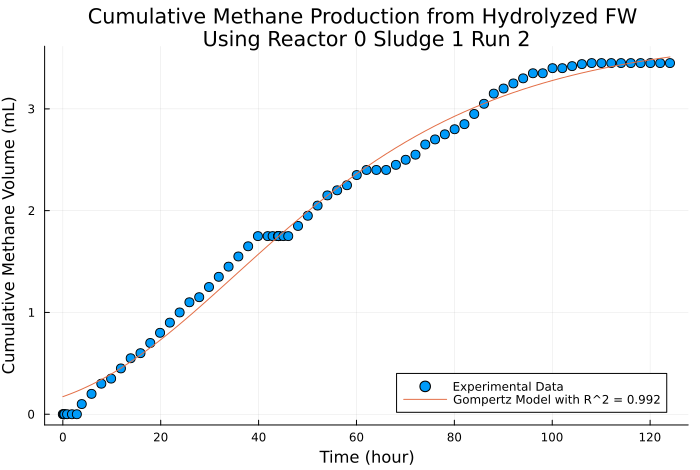
\includegraphics[width=.9\linewidth]{../plots/BMPs/Hydrolyzed FW/methane_kinetics_hydrolysate_0_s1_r2_hour.png}
\end{center}

\begin{center}
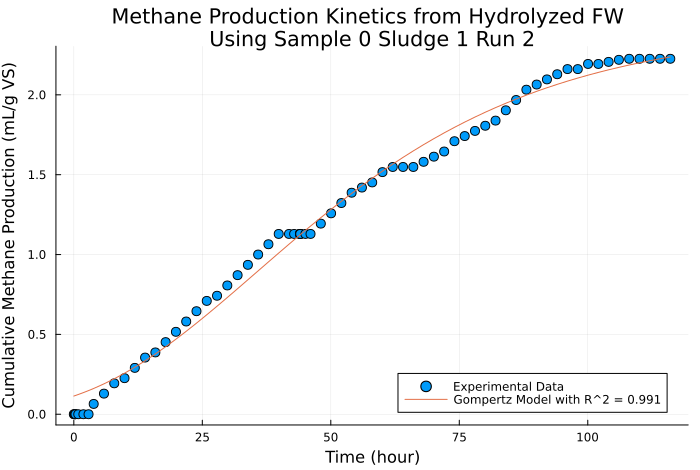
\includegraphics[width=.9\linewidth]{../plots/BMPs/Hydrolyzed FW/specific_methane_kinetics_hydrolysate_0_s1_r2_hour.png}
\end{center}

\subsection{Reactor 1}
\label{sec:orgd3d69ab}
Το δείγμα αυτό τροφοδοτήθηκε με το υδρόλυμα το οποίο είχε προσθήκη 1 ml mix. Στο αρχικό κινητικό πείραμα, το δείγμα αυτό είχε αρκετά παρόμοια συμπεριφορά με το 0 και χειρότερη αυτής του 1. Από την μέτρηση του COD του, είχε αναπάντεχα υψηλό sCOD. Αυτό σημαίνει είτε πως έγινε κάποιο λάθος στην ανάλυση ή ότι απλώς έγινε πολύ καλύτερη υδρόλυση από ότι περιμέναμε στο πείραμα αυτό. Με βάση το sCOD του, αναμένεται να έχει καλά αποτελέσματα. Με βάση την HPLC του αρχικού πειράματος, θα περιμέναμε να είναι λίγο καλύτερο από το 0.

\textbf{hydrolysate\textsubscript{1}\textsubscript{s1}\textsubscript{r2}}
\begin{minted}[breaklines=true,breakanywhere=true]{julia}

### Data Analysis on Hydrolysate with 1 ml ###

<<date_saving_fw_s1_r2>>

inds = 2:75
exp_meth_vol = [0, 0, 0, 0, 0, 0.2, 0.2, 0.2, 0.2, 0.2, 0.2, 0.2, 0.2, 0.2, 0.2, 0.2, 0.2, 0.2, 0.2, 0.2, 0.2, 0.05, 0.1, 0.2, 0.2, 0.2, 0.2, 0.1, 0.05, 0.1, 0, 0, 0, 0.1, 0.1, 0.2, 0.4, 0.5, 0.2, 0.1, 0.1, 0.2, 0, 0.1, 0.2, 0.2, 0.1, 0.3, 0.1, 0.1, 0, 0.1, 0.2, 0.2, 0.1, 0.2, 0.2, 0.1, 0.1, 0, 0.1, 0.2, 0, 0.1, 0.1, 0.2, 0.2, 0.1, 0, 0, 0, 0, 0, 0]
meth_vol_hydro_1 = cumsum(exp_meth_vol)[end]
exp_name = "hydrolysate_1_s1_r2"
source = "Hydrolyzed FW"
reactor = "Reactor 1"
sludge = "Sludge 1"
run_num = "Run 2"
input_vs = 1.5

p0 = [13.0, 1.0, 1.0]
<<bmp_data_processing>>
max_rate_hydro_1 = max_manual_rate

<<bmp_curve_fitting_min>>
model_hydro_1_min = vcat(reactor, round.(model_params, digits = 4), round(r_squared, digits = 3))
<<bmp_data_plotting>>

p0 = [20.0, 0.5, 1.0]
<<bmp_curve_fitting_hour>>
model_hydro_1_hour = vcat(reactor, round.(model_params, digits = 3), round(r_squared, digits = 3))
<<bmp_data_plotting>>

<<sma_curve_fitting_hour>>
sma_hydro_1 = vcat(reactor, round.(model_params, digits = 3), round(r_squared, digits = 3))
<<bmp_data_plotting>>

return("../data/exp_pro/"*exp_name*".csv")
\end{minted}

\subsubsection{Results}
\label{sec:orgef6049b}

\begin{minted}[breaklines=true,breakanywhere=true]{elisp}
(org-table-import-after-n-lines 3 <<hydrolysate_1_s1_r2()>> '(4))
\end{minted}

\begin{center}
\begin{tabular}{lrrrr}
Timestamp & Minutes & Hours & Methane\textsubscript{Volume} & Cumulative\textsubscript{Methane}\textsubscript{Volume}\\[0pt]
03/04\textsubscript{14}:45 & 0.0 & 0.0 & 0.0 & 0.0\\[0pt]
03/04\textsubscript{14}:51 & 6.137 & 0.1023 & 0.0 & 0.0\\[0pt]
03/04\textsubscript{14}:56 & 11.1825 & 0.1864 & 0.0 & 0.0\\[0pt]
03/04\textsubscript{15}:29 & 43.4534 & 0.7242 & 0.0 & 0.0\\[0pt]
03/04\textsubscript{16}:29 & 103.4538 & 1.7242 & 0.0 & 0.0\\[0pt]
03/04\textsubscript{17}:29 & 163.4582 & 2.7243 & 0.2 & 0.2\\[0pt]
03/04\textsubscript{18}:29 & 223.4582 & 3.7243 & 0.2 & 0.4\\[0pt]
03/04\textsubscript{20}:29 & 343.4582 & 5.7243 & 0.2 & 0.6\\[0pt]
03/04\textsubscript{22}:29 & 463.4582 & 7.7243 & 0.2 & 0.8\\[0pt]
04/04\textsubscript{00}:29 & 583.4649 & 9.7244 & 0.2 & 1.0\\[0pt]
04/04\textsubscript{02}:29 & 703.4649 & 11.7244 & 0.2 & 1.2\\[0pt]
04/04\textsubscript{04}:29 & 823.465 & 13.7244 & 0.2 & 1.4\\[0pt]
04/04\textsubscript{06}:29 & 943.4649 & 15.7244 & 0.2 & 1.6\\[0pt]
04/04\textsubscript{08}:29 & 1063.469 & 17.7245 & 0.2 & 1.8\\[0pt]
04/04\textsubscript{10}:29 & 1183.4749 & 19.7246 & 0.2 & 2.0\\[0pt]
04/04\textsubscript{12}:29 & 1303.4754 & 21.7246 & 0.2 & 2.2\\[0pt]
04/04\textsubscript{14}:29 & 1423.4755 & 23.7246 & 0.2 & 2.4\\[0pt]
04/04\textsubscript{16}:29 & 1543.4754 & 25.7246 & 0.2 & 2.6\\[0pt]
04/04\textsubscript{18}:29 & 1663.4938 & 27.7249 & 0.2 & 2.8\\[0pt]
04/04\textsubscript{20}:29 & 1783.4966 & 29.7249 & 0.2 & 3.0\\[0pt]
04/04\textsubscript{22}:29 & 1903.4979 & 31.725 & 0.2 & 3.2\\[0pt]
05/04\textsubscript{00}:29 & 2023.493 & 33.7249 & 0.05 & 3.25\\[0pt]
05/04\textsubscript{02}:29 & 2143.4939 & 35.7249 & 0.1 & 3.35\\[0pt]
05/04\textsubscript{04}:29 & 2263.4969 & 37.7249 & 0.2 & 3.55\\[0pt]
05/04\textsubscript{06}:29 & 2383.4976 & 39.725 & 0.2 & 3.75\\[0pt]
05/04\textsubscript{08}:29 & 2503.4975 & 41.725 & 0.2 & 3.95\\[0pt]
05/04\textsubscript{09}:29 & 2563.4972 & 42.725 & 0.2 & 4.15\\[0pt]
05/04\textsubscript{10}:37 & 2631.7736 & 43.8629 & 0.1 & 4.25\\[0pt]
05/04\textsubscript{10}:38 & 2632.7736 & 43.8796 & 0.05 & 4.3\\[0pt]
05/04\textsubscript{10}:39 & 2633.7736 & 43.8962 & 0.1 & 4.4\\[0pt]
05/04\textsubscript{10}:40 & 2634.7504 & 43.9125 & 0.0 & 4.4\\[0pt]
05/04\textsubscript{11}:40 & 2694.9257 & 44.9154 & 0.0 & 4.4\\[0pt]
05/04\textsubscript{12}:40 & 2754.9315 & 45.9155 & 0.0 & 4.4\\[0pt]
05/04\textsubscript{14}:40 & 2874.9314 & 47.9155 & 0.1 & 4.5\\[0pt]
05/04\textsubscript{16}:40 & 2994.9319 & 49.9155 & 0.1 & 4.6\\[0pt]
05/04\textsubscript{18}:40 & 3114.9378 & 51.9156 & 0.2 & 4.8\\[0pt]
05/04\textsubscript{20}:40 & 3234.9387 & 53.9156 & 0.4 & 5.2\\[0pt]
05/04\textsubscript{22}:40 & 3354.9413 & 55.9157 & 0.5 & 5.7\\[0pt]
06/04\textsubscript{00}:40 & 3474.945 & 57.9157 & 0.2 & 5.9\\[0pt]
06/04\textsubscript{02}:40 & 3594.9452 & 59.9158 & 0.1 & 6.0\\[0pt]
06/04\textsubscript{04}:40 & 3714.9451 & 61.9158 & 0.1 & 6.1\\[0pt]
06/04\textsubscript{06}:40 & 3834.9504 & 63.9158 & 0.2 & 6.3\\[0pt]
06/04\textsubscript{08}:40 & 3954.9524 & 65.9159 & 0.0 & 6.3\\[0pt]
06/04\textsubscript{10}:40 & 4074.9524 & 67.9159 & 0.1 & 6.4\\[0pt]
06/04\textsubscript{12}:40 & 4194.9604 & 69.916 & 0.2 & 6.6\\[0pt]
06/04\textsubscript{14}:40 & 4314.9606 & 71.916 & 0.2 & 6.8\\[0pt]
06/04\textsubscript{16}:40 & 4434.9633 & 73.9161 & 0.1 & 6.9\\[0pt]
06/04\textsubscript{18}:40 & 4554.964 & 75.9161 & 0.3 & 7.2\\[0pt]
06/04\textsubscript{20}:40 & 4674.9641 & 77.9161 & 0.1 & 7.3\\[0pt]
06/04\textsubscript{22}:40 & 4794.9641 & 79.9161 & 0.1 & 7.4\\[0pt]
07/04\textsubscript{00}:40 & 4914.9743 & 81.9162 & 0.0 & 7.4\\[0pt]
07/04\textsubscript{02}:40 & 5034.9749 & 83.9162 & 0.1 & 7.5\\[0pt]
07/04\textsubscript{04}:40 & 5154.975 & 85.9163 & 0.2 & 7.7\\[0pt]
07/04\textsubscript{06}:40 & 5274.9749 & 87.9162 & 0.2 & 7.9\\[0pt]
07/04\textsubscript{08}:40 & 5394.9769 & 89.9163 & 0.1 & 8.0\\[0pt]
07/04\textsubscript{10}:40 & 5514.9863 & 91.9164 & 0.2 & 8.2\\[0pt]
07/04\textsubscript{12}:40 & 5634.9883 & 93.9165 & 0.2 & 8.4\\[0pt]
07/04\textsubscript{14}:40 & 5754.9898 & 95.9165 & 0.1 & 8.5\\[0pt]
07/04\textsubscript{16}:40 & 5874.9911 & 97.9165 & 0.1 & 8.6\\[0pt]
07/04\textsubscript{18}:40 & 5994.9974 & 99.9166 & 0.0 & 8.6\\[0pt]
07/04\textsubscript{20}:40 & 6114.9986 & 101.9166 & 0.1 & 8.7\\[0pt]
07/04\textsubscript{22}:40 & 6234.9998 & 103.9167 & 0.2 & 8.9\\[0pt]
08/04\textsubscript{00}:40 & 6355.0168 & 105.9169 & 0.0 & 8.9\\[0pt]
08/04\textsubscript{02}:40 & 6475.018 & 107.917 & 0.1 & 9.0\\[0pt]
08/04\textsubscript{04}:40 & 6595.0092 & 109.9168 & 0.1 & 9.1\\[0pt]
08/04\textsubscript{06}:40 & 6715.0084 & 111.9168 & 0.2 & 9.3\\[0pt]
08/04\textsubscript{08}:40 & 6835.0084 & 113.9168 & 0.2 & 9.5\\[0pt]
08/04\textsubscript{10}:40 & 6955.0083 & 115.9168 & 0.1 & 9.6\\[0pt]
08/04\textsubscript{12}:40 & 7075.015 & 117.9169 & 0.0 & 9.6\\[0pt]
08/04\textsubscript{14}:40 & 7195.0183 & 119.917 & 0.0 & 9.6\\[0pt]
08/04\textsubscript{16}:40 & 7315.0187 & 121.917 & 0.0 & 9.6\\[0pt]
08/04\textsubscript{18}:40 & 7435.0194 & 123.917 & 0.0 & 9.6\\[0pt]
08/04\textsubscript{20}:40 & 7555.0196 & 125.917 & 0.0 & 9.6\\[0pt]
08/04\textsubscript{22}:40 & 7675.0303 & 127.9172 & 0.0 & 9.6\\[0pt]
\end{tabular}
\end{center}

\begin{center}
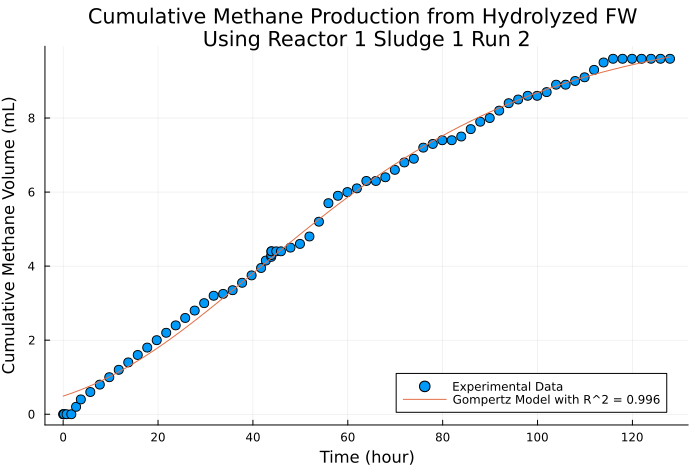
\includegraphics[width=.9\linewidth]{../plots/BMPs/Hydrolyzed FW/methane_kinetics_hydrolysate_1_s1_r2_hour.png}
\end{center}

\begin{center}
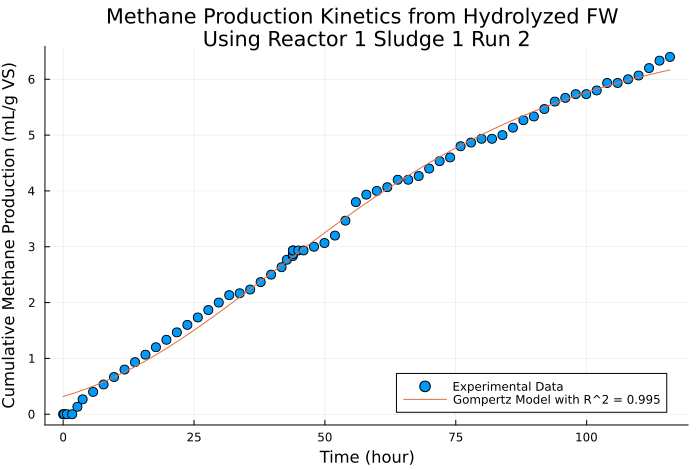
\includegraphics[width=.9\linewidth]{../plots/BMPs/Hydrolyzed FW/specific_methane_kinetics_hydrolysate_1_s1_r2_hour.png}
\end{center}

\subsection{Reactor 2}
\label{sec:orgb33c9e7}
Το δείγμα το οποίο στην υδρόλυση είχε 2 ml από το μιξ. Με βάση το αρχικό πείραμα υδρόλυσης, αυτό και το 4 ml είχαν το καλύτερο performance και ελάχιστη διαφορά μεταξύ τους (κατά βάση στην συγκέντρωση γαλακτικού οξέος) οπότε θα αναμέναμε εδώ να παρατηρηθεί η καλύτερη μεθανογένεση.

\textbf{hydrolysate\textsubscript{2}\textsubscript{s1}\textsubscript{r2}}
\begin{minted}[breaklines=true,breakanywhere=true]{julia}

### Data Analysis on Hydrolysate with 2 ml ###

<<date_saving_fw_s1_r2>>

inds = 3:74
exp_meth_vol = [0, 0, 0.05, 1.2, 0.2, 0.2, 0.1, 0.4, 0.5, 0.2, 0.1, 0.5, 0, 0.1, 0.2, 0.2, 0.2, 0.1, 0.05, 0.05, 0.05, 0, 0.1, 0.1, 0, 0, 0, 0.1, 0.1, 0.2, 0.05, 0, 0.1, 0.1, 0.1, 0.1, 0.1, 0.1, 0.2, 0.2, 0.2, 0.2, 0.1, 0.05, 0.05, 0, 0.05, 0.1, 0.1, 0, 0.05, 0.1, 0.1, 0.2, 0.2, 0, 0.1, 0.1, 0, 0, 0, 0, 0, 0, 0.05, 0.05, 0.05, 0, 0, 0, 0, 0]
meth_vol_hydro_2 = cumsum(exp_meth_vol)[end]
exp_name = "hydrolysate_2_s1_r2"
source = "Hydrolyzed FW"
reactor = "Reactor 2"
sludge = "Sludge 1"
run_num = "Run 2"
input_vs = 1.55

<<bmp_data_processing>>
max_rate_hydro_2 = max_manual_rate

p0 = [10.0, 1.50, 1.0]
<<bmp_curve_fitting_min>>
model_hydro_2_min = vcat(reactor, round.(model_params, digits = 4), round(r_squared, digits = 3))
<<bmp_data_plotting>>

p0 = [10.0, 0.1, 0.03]
<<bmp_curve_fitting_hour>>
model_hydro_2_hour = vcat(reactor, round.(model_params, digits = 3), round(r_squared, digits = 3))
<<bmp_data_plotting>>

<<sma_curve_fitting_hour>>
sma_hydro_2 = vcat(reactor, round.(model_params, digits = 3), round(r_squared, digits = 3))
<<bmp_data_plotting>>

return("../data/exp_pro/"*exp_name*".csv")
\end{minted}

\subsubsection{Results}
\label{sec:org6a227e6}

\begin{minted}[breaklines=true,breakanywhere=true]{elisp}
(org-table-import-after-n-lines 3 <<hydrolysate_2_s1_r2()>> '(4))
\end{minted}

\begin{center}
\begin{tabular}{lrrrr}
Timestamp & Minutes & Hours & Methane\textsubscript{Volume} & Cumulative\textsubscript{Methane}\textsubscript{Volume}\\[0pt]
03/04\textsubscript{14}:56 & 0.0 & 0.0 & 0.0 & 0.0\\[0pt]
03/04\textsubscript{15}:29 & 32.2709 & 0.5378 & 0.1 & 0.1\\[0pt]
03/04\textsubscript{16}:29 & 92.2712 & 1.5379 & 0.1 & 0.2\\[0pt]
03/04\textsubscript{17}:29 & 152.2757 & 2.5379 & 1.3 & 1.5\\[0pt]
03/04\textsubscript{18}:29 & 212.2757 & 3.5379 & 0.0 & 1.5\\[0pt]
03/04\textsubscript{20}:29 & 332.2757 & 5.5379 & 0.2 & 1.7\\[0pt]
03/04\textsubscript{22}:29 & 452.2757 & 7.5379 & 0.1 & 1.8\\[0pt]
04/04\textsubscript{00}:29 & 572.2824 & 9.538 & 0.4 & 2.2\\[0pt]
04/04\textsubscript{02}:29 & 692.2824 & 11.538 & 0.5 & 2.7\\[0pt]
04/04\textsubscript{04}:29 & 812.2825 & 13.538 & 0.2 & 2.9\\[0pt]
04/04\textsubscript{06}:29 & 932.2824 & 15.538 & 0.1 & 3.0\\[0pt]
04/04\textsubscript{08}:29 & 1052.2865 & 17.5381 & 0.5 & 3.5\\[0pt]
04/04\textsubscript{10}:29 & 1172.2924 & 19.5382 & 0.0 & 3.5\\[0pt]
04/04\textsubscript{12}:29 & 1292.2929 & 21.5382 & 0.1 & 3.6\\[0pt]
04/04\textsubscript{14}:29 & 1412.293 & 23.5382 & 0.2 & 3.8\\[0pt]
04/04\textsubscript{16}:29 & 1532.2929 & 25.5382 & 0.2 & 4.0\\[0pt]
04/04\textsubscript{18}:29 & 1652.3113 & 27.5385 & 0.2 & 4.2\\[0pt]
04/04\textsubscript{20}:29 & 1772.3141 & 29.5386 & 0.1 & 4.3\\[0pt]
04/04\textsubscript{22}:29 & 1892.3154 & 31.5386 & 0.05 & 4.35\\[0pt]
05/04\textsubscript{00}:29 & 2012.3105 & 33.5385 & 0.05 & 4.4\\[0pt]
05/04\textsubscript{02}:29 & 2132.3114 & 35.5385 & 0.05 & 4.45\\[0pt]
05/04\textsubscript{04}:29 & 2252.3144 & 37.5386 & 0.0 & 4.45\\[0pt]
05/04\textsubscript{06}:29 & 2372.3151 & 39.5386 & 0.1 & 4.55\\[0pt]
05/04\textsubscript{08}:29 & 2492.315 & 41.5386 & 0.1 & 4.65\\[0pt]
05/04\textsubscript{09}:29 & 2552.3147 & 42.5386 & 0.0 & 4.65\\[0pt]
05/04\textsubscript{10}:37 & 2620.5911 & 43.6765 & 0.0 & 4.65\\[0pt]
05/04\textsubscript{10}:38 & 2621.5911 & 43.6932 & 0.0 & 4.65\\[0pt]
05/04\textsubscript{10}:39 & 2622.5911 & 43.7099 & 0.1 & 4.75\\[0pt]
05/04\textsubscript{10}:40 & 2623.568 & 43.7261 & 0.1 & 4.85\\[0pt]
05/04\textsubscript{11}:40 & 2683.7432 & 44.7291 & 0.2 & 5.05\\[0pt]
05/04\textsubscript{12}:40 & 2743.749 & 45.7292 & 0.05 & 5.1\\[0pt]
05/04\textsubscript{14}:40 & 2863.749 & 47.7291 & 0.0 & 5.1\\[0pt]
05/04\textsubscript{16}:40 & 2983.7494 & 49.7292 & 0.1 & 5.2\\[0pt]
05/04\textsubscript{18}:40 & 3103.7554 & 51.7293 & 0.1 & 5.3\\[0pt]
05/04\textsubscript{20}:40 & 3223.7562 & 53.7293 & 0.1 & 5.4\\[0pt]
05/04\textsubscript{22}:40 & 3343.7588 & 55.7293 & 0.1 & 5.5\\[0pt]
06/04\textsubscript{00}:40 & 3463.7624 & 57.7294 & 0.1 & 5.6\\[0pt]
06/04\textsubscript{02}:40 & 3583.7627 & 59.7294 & 0.1 & 5.7\\[0pt]
06/04\textsubscript{04}:40 & 3703.7626 & 61.7294 & 0.2 & 5.9\\[0pt]
06/04\textsubscript{06}:40 & 3823.768 & 63.7295 & 0.2 & 6.1\\[0pt]
06/04\textsubscript{08}:40 & 3943.77 & 65.7295 & 0.2 & 6.3\\[0pt]
06/04\textsubscript{10}:40 & 4063.7699 & 67.7295 & 0.2 & 6.5\\[0pt]
06/04\textsubscript{12}:40 & 4183.7779 & 69.7296 & 0.1 & 6.6\\[0pt]
06/04\textsubscript{14}:40 & 4303.7782 & 71.7296 & 0.05 & 6.65\\[0pt]
06/04\textsubscript{16}:40 & 4423.7808 & 73.7297 & 0.05 & 6.7\\[0pt]
06/04\textsubscript{18}:40 & 4543.7815 & 75.7297 & 0.0 & 6.7\\[0pt]
06/04\textsubscript{20}:40 & 4663.7816 & 77.7297 & 0.05 & 6.75\\[0pt]
06/04\textsubscript{22}:40 & 4783.7816 & 79.7297 & 0.1 & 6.85\\[0pt]
07/04\textsubscript{00}:40 & 4903.7918 & 81.7299 & 0.1 & 6.95\\[0pt]
07/04\textsubscript{02}:40 & 5023.7924 & 83.7299 & 0.0 & 6.95\\[0pt]
07/04\textsubscript{04}:40 & 5143.7925 & 85.7299 & 0.05 & 7.0\\[0pt]
07/04\textsubscript{06}:40 & 5263.7924 & 87.7299 & 0.1 & 7.1\\[0pt]
07/04\textsubscript{08}:40 & 5383.7944 & 89.7299 & 0.1 & 7.2\\[0pt]
07/04\textsubscript{10}:40 & 5503.8038 & 91.7301 & 0.2 & 7.4\\[0pt]
07/04\textsubscript{12}:40 & 5623.8058 & 93.7301 & 0.2 & 7.6\\[0pt]
07/04\textsubscript{14}:40 & 5743.8073 & 95.7301 & 0.0 & 7.6\\[0pt]
07/04\textsubscript{16}:40 & 5863.8086 & 97.7301 & 0.1 & 7.7\\[0pt]
07/04\textsubscript{18}:40 & 5983.8149 & 99.7302 & 0.1 & 7.8\\[0pt]
07/04\textsubscript{20}:40 & 6103.8161 & 101.7303 & 0.0 & 7.8\\[0pt]
07/04\textsubscript{22}:40 & 6223.8172 & 103.7303 & 0.0 & 7.8\\[0pt]
08/04\textsubscript{00}:40 & 6343.8343 & 105.7306 & 0.0 & 7.8\\[0pt]
08/04\textsubscript{02}:40 & 6463.8355 & 107.7306 & 0.0 & 7.8\\[0pt]
08/04\textsubscript{04}:40 & 6583.8267 & 109.7304 & 0.0 & 7.8\\[0pt]
08/04\textsubscript{06}:40 & 6703.826 & 111.7304 & 0.0 & 7.8\\[0pt]
08/04\textsubscript{08}:40 & 6823.8259 & 113.7304 & 0.05 & 7.85\\[0pt]
08/04\textsubscript{10}:40 & 6943.8258 & 115.7304 & 0.05 & 7.9\\[0pt]
08/04\textsubscript{12}:40 & 7063.8325 & 117.7305 & 0.05 & 7.95\\[0pt]
08/04\textsubscript{14}:40 & 7183.8358 & 119.7306 & 0.0 & 7.95\\[0pt]
08/04\textsubscript{16}:40 & 7303.8362 & 121.7306 & 0.0 & 7.95\\[0pt]
08/04\textsubscript{18}:40 & 7423.837 & 123.7306 & 0.0 & 7.95\\[0pt]
08/04\textsubscript{20}:40 & 7543.837 & 125.7306 & 0.0 & 7.95\\[0pt]
08/04\textsubscript{22}:40 & 7663.8478 & 127.7308 & 0.0 & 7.95\\[0pt]
\end{tabular}
\end{center}


\begin{center}
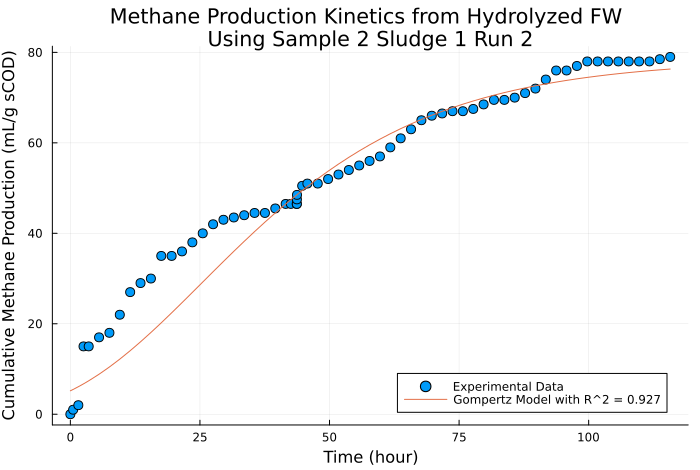
\includegraphics[width=.9\linewidth]{../plots/BMPs/Hydrolyzed FW/methane_kinetics_hydrolysate_2_s1_r2_hour.png}
\end{center}

\begin{center}
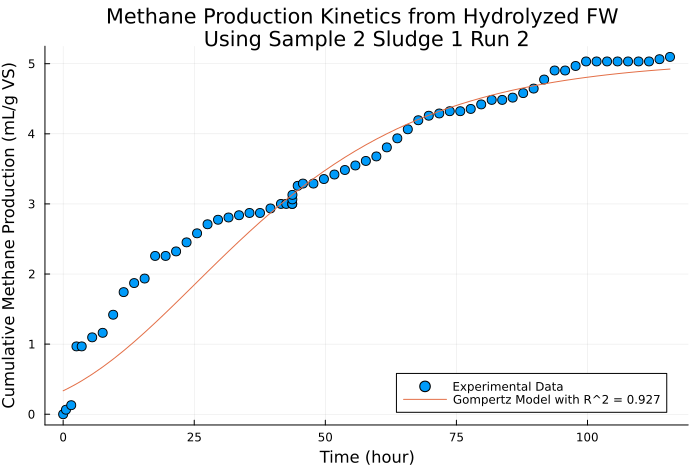
\includegraphics[width=.9\linewidth]{../plots/BMPs/Hydrolyzed FW/specific_methane_kinetics_hydrolysate_2_s1_r2_hour.png}
\end{center}

\subsection{Reactor 4}
\label{sec:orgec954b8}
Το δείγμα 4 ήταν αυτό με τα 4 ml mix στην υδρόλυση. Είναι η μέγιστη ποσότητα που χρησιμοποιήθηκε για τα πειράματα χώνευσης καθώς το 8 ml δεν είχε ιδιαίτερα μεγάλη διαφορά και είναι πολύ πιο ακριβό. Όπως προαναφέρθηκε, αναμένουμε να έχει παρόμοια ποιότητα με το 2 ml καθώς με εξαίρεση μίας ποσότητας γαλακτικού είναι σχεδόν ίδια.

\textbf{hydrolysate\textsubscript{4}\textsubscript{s1}\textsubscript{r2}}
\begin{minted}[breaklines=true,breakanywhere=true]{julia}

### Data Analysis on Hydrolysate with 4 ml ###

<<date_saving_fw_s1_r2>>

inds = 3:75
exp_meth_vol = [0, 0, 0, 0, 0.05, 0.1, 0.1, 0.3, 0.3, 0.3, 0.3, 0.3, 0.1, 0.2, 0.1, 0.1, 0.2, 0.1, 0.1, 0.05, 0.1, 0.2, 0.2, 0.1, 0.05, 0.1, 0.1, 0, 0, 0, 0, 0.1, 0.1, 0.2, 0.1, 0.1, 0.1, 0.1, 0.1, 0.1, 0.2, 0.1, 0.1, 0.2, 0.1, 0.2, 0.1, 0.1, 0.1, 0.1, 0.1, 0.2, 0.1, 0.1, 0.1, 0.1, 0.1, 0.2, 0.2, 0.1, 0, 0, 0.05, 0.05, 0, 0.05, 0.1, 0, 0, 0, 0, 0, 0]
meth_vol_hydro_4 = cumsum(exp_meth_vol)[end]
exp_name = "hydrolysate_4_s1_r2"
source = "Hydrolyzed FW"
reactor = "Reactor 4"
sludge = "Sludge 1"
run_num = "Run 2"

input_vs = 1.55

<<bmp_data_processing>>
max_rate_hydro_4 = max_manual_rate

p0 = [17.0, 15.0, 1.0]
<<bmp_curve_fitting_min>>
model_hydro_4_min = vcat(reactor, round.(model_params, digits = 4), round(r_squared, digits = 3))
<<bmp_data_plotting>>

p0 = [17.0, 100.0, 0.1]
<<bmp_curve_fitting_hour>>
model_hydro_4_hour = vcat(reactor, round.(model_params, digits = 3), round(r_squared, digits = 3))
<<bmp_data_plotting>>

<<sma_curve_fitting_hour>>
sma_hydro_4 = vcat(reactor, round.(model_params, digits = 3), round(r_squared, digits = 3))
<<bmp_data_plotting>>

return("../data/exp_pro/"*exp_name*".csv")
\end{minted}

\subsubsection{Results}
\label{sec:org8379963}

\begin{minted}[breaklines=true,breakanywhere=true]{elisp}
(org-table-import-after-n-lines 3 <<hydrolysate_4_s1_r2()>> '(4))
\end{minted}

\begin{center}
\begin{tabular}{lrrrr}
Timestamp & Minutes & Hours & Methane\textsubscript{Volume} & Cumulative\textsubscript{Methane}\textsubscript{Volume}\\[0pt]
03/04\textsubscript{14}:51 & 0.0 & 0.0 & 0.0 & 0.0\\[0pt]
03/04\textsubscript{14}:56 & 5.0455 & 0.0841 & 0.0 & 0.0\\[0pt]
03/04\textsubscript{15}:29 & 37.3164 & 0.6219 & 0.0 & 0.0\\[0pt]
03/04\textsubscript{16}:29 & 97.3168 & 1.6219 & 0.0 & 0.0\\[0pt]
03/04\textsubscript{17}:29 & 157.3212 & 2.622 & 0.05 & 0.05\\[0pt]
03/04\textsubscript{18}:29 & 217.3212 & 3.622 & 0.1 & 0.15\\[0pt]
03/04\textsubscript{20}:29 & 337.3212 & 5.622 & 0.1 & 0.25\\[0pt]
03/04\textsubscript{22}:29 & 457.3212 & 7.622 & 0.3 & 0.55\\[0pt]
04/04\textsubscript{00}:29 & 577.3279 & 9.6221 & 0.3 & 0.85\\[0pt]
04/04\textsubscript{02}:29 & 697.3279 & 11.6221 & 0.3 & 1.15\\[0pt]
04/04\textsubscript{04}:29 & 817.328 & 13.6221 & 0.3 & 1.45\\[0pt]
04/04\textsubscript{06}:29 & 937.3279 & 15.6221 & 0.3 & 1.75\\[0pt]
04/04\textsubscript{08}:29 & 1057.332 & 17.6222 & 0.1 & 1.85\\[0pt]
04/04\textsubscript{10}:29 & 1177.3379 & 19.6223 & 0.2 & 2.05\\[0pt]
04/04\textsubscript{12}:29 & 1297.3384 & 21.6223 & 0.1 & 2.15\\[0pt]
04/04\textsubscript{14}:29 & 1417.3385 & 23.6223 & 0.1 & 2.25\\[0pt]
04/04\textsubscript{16}:29 & 1537.3384 & 25.6223 & 0.2 & 2.45\\[0pt]
04/04\textsubscript{18}:29 & 1657.3568 & 27.6226 & 0.1 & 2.55\\[0pt]
04/04\textsubscript{20}:29 & 1777.3596 & 29.6227 & 0.1 & 2.65\\[0pt]
04/04\textsubscript{22}:29 & 1897.3609 & 31.6227 & 0.05 & 2.7\\[0pt]
05/04\textsubscript{00}:29 & 2017.356 & 33.6226 & 0.1 & 2.8\\[0pt]
05/04\textsubscript{02}:29 & 2137.3569 & 35.6226 & 0.2 & 3.0\\[0pt]
05/04\textsubscript{04}:29 & 2257.3599 & 37.6227 & 0.2 & 3.2\\[0pt]
05/04\textsubscript{06}:29 & 2377.3606 & 39.6227 & 0.1 & 3.3\\[0pt]
05/04\textsubscript{08}:29 & 2497.3605 & 41.6227 & 0.05 & 3.35\\[0pt]
05/04\textsubscript{09}:29 & 2557.3602 & 42.6227 & 0.1 & 3.45\\[0pt]
05/04\textsubscript{10}:37 & 2625.6366 & 43.7606 & 0.1 & 3.55\\[0pt]
05/04\textsubscript{10}:38 & 2626.6366 & 43.7773 & 0.0 & 3.55\\[0pt]
05/04\textsubscript{10}:39 & 2627.6366 & 43.7939 & 0.0 & 3.55\\[0pt]
05/04\textsubscript{10}:40 & 2628.6134 & 43.8102 & 0.0 & 3.55\\[0pt]
05/04\textsubscript{11}:40 & 2688.7887 & 44.8131 & 0.0 & 3.55\\[0pt]
05/04\textsubscript{12}:40 & 2748.7945 & 45.8132 & 0.1 & 3.65\\[0pt]
05/04\textsubscript{14}:40 & 2868.7944 & 47.8132 & 0.1 & 3.75\\[0pt]
05/04\textsubscript{16}:40 & 2988.7949 & 49.8132 & 0.2 & 3.95\\[0pt]
05/04\textsubscript{18}:40 & 3108.8008 & 51.8133 & 0.1 & 4.05\\[0pt]
05/04\textsubscript{20}:40 & 3228.8017 & 53.8134 & 0.1 & 4.15\\[0pt]
05/04\textsubscript{22}:40 & 3348.8043 & 55.8134 & 0.1 & 4.25\\[0pt]
06/04\textsubscript{00}:40 & 3468.808 & 57.8135 & 0.1 & 4.35\\[0pt]
06/04\textsubscript{02}:40 & 3588.8082 & 59.8135 & 0.1 & 4.45\\[0pt]
06/04\textsubscript{04}:40 & 3708.8081 & 61.8135 & 0.1 & 4.55\\[0pt]
06/04\textsubscript{06}:40 & 3828.8134 & 63.8136 & 0.2 & 4.75\\[0pt]
06/04\textsubscript{08}:40 & 3948.8154 & 65.8136 & 0.1 & 4.85\\[0pt]
06/04\textsubscript{10}:40 & 4068.8154 & 67.8136 & 0.1 & 4.95\\[0pt]
06/04\textsubscript{12}:40 & 4188.8234 & 69.8137 & 0.2 & 5.15\\[0pt]
06/04\textsubscript{14}:40 & 4308.8236 & 71.8137 & 0.1 & 5.25\\[0pt]
06/04\textsubscript{16}:40 & 4428.8263 & 73.8138 & 0.2 & 5.45\\[0pt]
06/04\textsubscript{18}:40 & 4548.827 & 75.8138 & 0.1 & 5.55\\[0pt]
06/04\textsubscript{20}:40 & 4668.8271 & 77.8138 & 0.1 & 5.65\\[0pt]
06/04\textsubscript{22}:40 & 4788.8271 & 79.8138 & 0.1 & 5.75\\[0pt]
07/04\textsubscript{00}:40 & 4908.8373 & 81.814 & 0.1 & 5.85\\[0pt]
07/04\textsubscript{02}:40 & 5028.8379 & 83.814 & 0.1 & 5.95\\[0pt]
07/04\textsubscript{04}:40 & 5148.838 & 85.814 & 0.2 & 6.15\\[0pt]
07/04\textsubscript{06}:40 & 5268.8379 & 87.814 & 0.1 & 6.25\\[0pt]
07/04\textsubscript{08}:40 & 5388.8399 & 89.814 & 0.1 & 6.35\\[0pt]
07/04\textsubscript{10}:40 & 5508.8493 & 91.8142 & 0.1 & 6.45\\[0pt]
07/04\textsubscript{12}:40 & 5628.8513 & 93.8142 & 0.1 & 6.55\\[0pt]
07/04\textsubscript{14}:40 & 5748.8528 & 95.8142 & 0.1 & 6.65\\[0pt]
07/04\textsubscript{16}:40 & 5868.8541 & 97.8142 & 0.2 & 6.85\\[0pt]
07/04\textsubscript{18}:40 & 5988.8604 & 99.8143 & 0.2 & 7.05\\[0pt]
07/04\textsubscript{20}:40 & 6108.8616 & 101.8144 & 0.1 & 7.15\\[0pt]
07/04\textsubscript{22}:40 & 6228.8628 & 103.8144 & 0.0 & 7.15\\[0pt]
08/04\textsubscript{00}:40 & 6348.8798 & 105.8147 & 0.0 & 7.15\\[0pt]
08/04\textsubscript{02}:40 & 6468.881 & 107.8147 & 0.05 & 7.2\\[0pt]
08/04\textsubscript{04}:40 & 6588.8722 & 109.8145 & 0.05 & 7.25\\[0pt]
08/04\textsubscript{06}:40 & 6708.8714 & 111.8145 & 0.0 & 7.25\\[0pt]
08/04\textsubscript{08}:40 & 6828.8714 & 113.8145 & 0.05 & 7.3\\[0pt]
08/04\textsubscript{10}:40 & 6948.8713 & 115.8145 & 0.1 & 7.4\\[0pt]
08/04\textsubscript{12}:40 & 7068.878 & 117.8146 & 0.0 & 7.4\\[0pt]
08/04\textsubscript{14}:40 & 7188.8813 & 119.8147 & 0.0 & 7.4\\[0pt]
08/04\textsubscript{16}:40 & 7308.8817 & 121.8147 & 0.0 & 7.4\\[0pt]
08/04\textsubscript{18}:40 & 7428.8824 & 123.8147 & 0.0 & 7.4\\[0pt]
08/04\textsubscript{20}:40 & 7548.8826 & 125.8147 & 0.0 & 7.4\\[0pt]
08/04\textsubscript{22}:40 & 7668.8933 & 127.8149 & 0.0 & 7.4\\[0pt]
\end{tabular}
\end{center}


\begin{center}
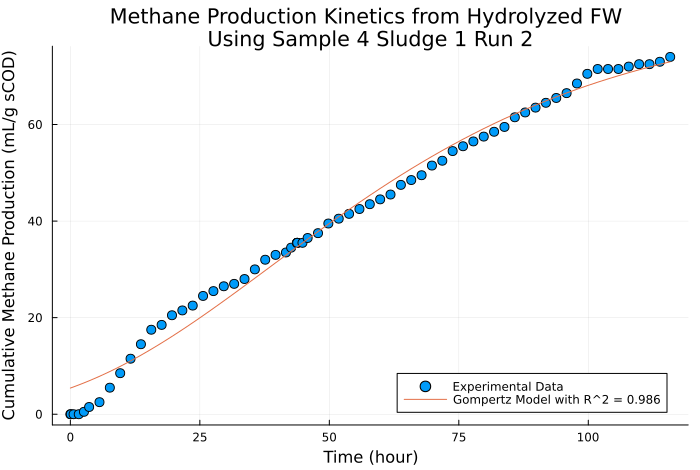
\includegraphics[width=.9\linewidth]{../plots/BMPs/Hydrolyzed FW/methane_kinetics_hydrolysate_4_s1_r2_hour.png}
\end{center}

\begin{center}
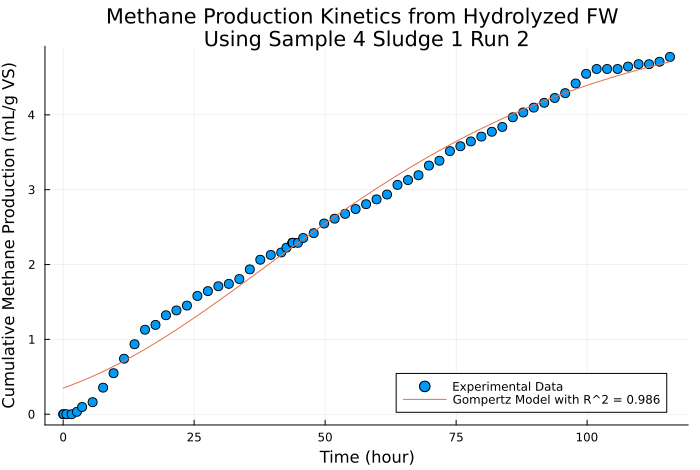
\includegraphics[width=.9\linewidth]{../plots/BMPs/Hydrolyzed FW/specific_methane_kinetics_hydrolysate_4_s1_r2_hour.png}
\end{center}

\subsection{Untreated FW}
\label{sec:org1f43219}
Εκτός από τα παραπάνω, σε ένα από τα δοχεία προστέθηκε ανεπεξέργαστο FW. Αυτό έχει διαφορά από το δείγμα 0, καθώς εκείνο υπέστει ζύμωση κατά τις 72 ώρες που ήταν στους 40 \(^oC\) ακόμη και χωρίς να προσθέσουμε κάποιο εμβόλιο, ενώ το δείγμα αυτό αναφέρεται σε food waste το οποίο δεν έχει υποστεί καμία επεξεργασία. Θα θέλαμε το δείγμα αυτό να έχει το χειρότερο performance (είτε πολύ αργή παραγωγή, ή μικρή τελική παραγωγή), το οποίο θα μας επιδείκνυε πως η επεξεργασία που έγινε βοηθάει πραγματικά στην χώνευση. Βέβαια, αξίζει να αναφερθεί πως το δοχείο αυτό είχε κάποιο προβλήματα με διαρροή στα αρχικά στάδια του πειράματος, οπότε ενδέχεται τα αποτελέσματα που θα προκύψουν να μην είναι έγκυρα. Παρακάτω φαίνεται ο κώδικας επεξεργασίας των αποτελεσμάτων του.

\textbf{untreated\textsubscript{fw}\textsubscript{s1}\textsubscript{r2}}
\begin{minted}[breaklines=true,breakanywhere=true]{julia}

### Data Analysis on Untreated FW ###
<<date_saving_fw_s1_r2>>

inds = 33:104
exp_meth_vol = vcat([0, 0, 0.1, 0.1, 0.1, 0.2, 0.2, 0.1, 0.1, 0.1, 0.1, 0.1, 0.05, 0.05, 0, 0, 0.2, 0.2, 0.1, 0.1, 0.1, 0, 0.1, 0.1, 0.1, 0.1, 0, 0.1, 0.05], zeros(43))
meth_vol_hydro_fw = cumsum(exp_meth_vol)[end]
exp_name = "untreated_fw_s1_r2"
source = "Untreated FW"
reactor = "FW"
sludge = "Sludge 1"
run_num = "Run 2"

input_vs = 1.55

<<bmp_data_processing>>
max_rate_hydro_fw = max_manual_rate

p0 = [2.5, 0.05, 1.0]
<<bmp_curve_fitting_min>>
model_hydro_fw_min = vcat(reactor, round.(model_params, digits = 4), round(r_squared, digits = 3))
<<bmp_data_plotting>>

p0 = [2.5, 0.1, 0.1]
<<bmp_curve_fitting_hour>>
model_hydro_fw_hour = vcat(reactor, round.(model_params, digits = 3), round(r_squared, digits = 3))
<<bmp_data_plotting>>

<<sma_curve_fitting_hour>>
sma_hydro_fw = vcat(reactor, round.(model_params, digits = 3), round(r_squared, digits = 3))
<<bmp_data_plotting>>

return("../data/exp_pro/"*exp_name*".csv")

\end{minted}

\subsubsection{Results}
\label{sec:org14dc996}

\begin{minted}[breaklines=true,breakanywhere=true]{elisp}
(org-table-import-after-n-lines 3 <<untreated_fw_s1_r2()>> '(4))
\end{minted}

\begin{center}
\begin{tabular}{lrrrr}
Timestamp & Minutes & Hours & Methane\textsubscript{Volume} & Cumulative\textsubscript{Methane}\textsubscript{Volume}\\[0pt]
05/04\textsubscript{11}:40 & 0.0 & 0.0 & 0.0 & 0.0\\[0pt]
05/04\textsubscript{12}:40 & 60.0058 & 1.0001 & 0.0 & 0.0\\[0pt]
05/04\textsubscript{14}:40 & 180.0058 & 3.0001 & 0.0 & 0.0\\[0pt]
05/04\textsubscript{16}:40 & 300.0062 & 5.0001 & 0.1 & 0.1\\[0pt]
05/04\textsubscript{18}:40 & 420.0122 & 7.0002 & 0.1 & 0.2\\[0pt]
05/04\textsubscript{20}:40 & 540.013 & 9.0002 & 0.2 & 0.4\\[0pt]
05/04\textsubscript{22}:40 & 660.0156 & 11.0003 & 0.2 & 0.6\\[0pt]
06/04\textsubscript{00}:40 & 780.0193 & 13.0003 & 0.1 & 0.7\\[0pt]
06/04\textsubscript{02}:40 & 900.0195 & 15.0003 & 0.1 & 0.8\\[0pt]
06/04\textsubscript{04}:40 & 1020.0194 & 17.0003 & 0.1 & 0.9\\[0pt]
06/04\textsubscript{06}:40 & 1140.0248 & 19.0004 & 0.1 & 1.0\\[0pt]
06/04\textsubscript{08}:40 & 1260.0268 & 21.0004 & 0.1 & 1.1\\[0pt]
06/04\textsubscript{10}:40 & 1380.0267 & 23.0004 & 0.05 & 1.15\\[0pt]
06/04\textsubscript{12}:40 & 1500.0347 & 25.0006 & 0.05 & 1.2\\[0pt]
06/04\textsubscript{14}:40 & 1620.035 & 27.0006 & 0.0 & 1.2\\[0pt]
06/04\textsubscript{16}:40 & 1740.0376 & 29.0006 & 0.0 & 1.2\\[0pt]
06/04\textsubscript{18}:40 & 1860.0382 & 31.0006 & 0.2 & 1.4\\[0pt]
06/04\textsubscript{20}:40 & 1980.0384 & 33.0006 & 0.2 & 1.6\\[0pt]
06/04\textsubscript{22}:40 & 2100.0384 & 35.0006 & 0.1 & 1.7\\[0pt]
07/04\textsubscript{00}:40 & 2220.0486 & 37.0008 & 0.1 & 1.8\\[0pt]
07/04\textsubscript{02}:40 & 2340.0492 & 39.0008 & 0.1 & 1.9\\[0pt]
07/04\textsubscript{04}:40 & 2460.0493 & 41.0008 & 0.0 & 1.9\\[0pt]
07/04\textsubscript{06}:40 & 2580.0492 & 43.0008 & 0.1 & 2.0\\[0pt]
07/04\textsubscript{08}:40 & 2700.0512 & 45.0009 & 0.1 & 2.1\\[0pt]
07/04\textsubscript{10}:40 & 2820.0606 & 47.001 & 0.1 & 2.2\\[0pt]
07/04\textsubscript{12}:40 & 2940.0626 & 49.001 & 0.1 & 2.3\\[0pt]
07/04\textsubscript{14}:40 & 3060.0641 & 51.0011 & 0.0 & 2.3\\[0pt]
07/04\textsubscript{16}:40 & 3180.0654 & 53.0011 & 0.1 & 2.4\\[0pt]
07/04\textsubscript{18}:40 & 3300.0717 & 55.0012 & 0.05 & 2.45\\[0pt]
07/04\textsubscript{20}:40 & 3420.0729 & 57.0012 & 0.0 & 2.45\\[0pt]
07/04\textsubscript{22}:40 & 3540.074 & 59.0012 & 0.0 & 2.45\\[0pt]
08/04\textsubscript{00}:40 & 3660.0911 & 61.0015 & 0.0 & 2.45\\[0pt]
08/04\textsubscript{02}:40 & 3780.0923 & 63.0015 & 0.0 & 2.45\\[0pt]
08/04\textsubscript{04}:40 & 3900.0835 & 65.0014 & 0.0 & 2.45\\[0pt]
08/04\textsubscript{06}:40 & 4020.0828 & 67.0014 & 0.0 & 2.45\\[0pt]
08/04\textsubscript{08}:40 & 4140.0827 & 69.0014 & 0.0 & 2.45\\[0pt]
08/04\textsubscript{10}:40 & 4260.0826 & 71.0014 & 0.0 & 2.45\\[0pt]
08/04\textsubscript{12}:40 & 4380.0893 & 73.0015 & 0.0 & 2.45\\[0pt]
08/04\textsubscript{14}:40 & 4500.0926 & 75.0015 & 0.0 & 2.45\\[0pt]
08/04\textsubscript{16}:40 & 4620.093 & 77.0015 & 0.0 & 2.45\\[0pt]
08/04\textsubscript{18}:40 & 4740.0938 & 79.0016 & 0.0 & 2.45\\[0pt]
08/04\textsubscript{20}:40 & 4860.0938 & 81.0016 & 0.0 & 2.45\\[0pt]
08/04\textsubscript{22}:40 & 4980.1046 & 83.0017 & 0.0 & 2.45\\[0pt]
08/04\textsubscript{23}:40 & 5040.107 & 84.0018 & 0.0 & 2.45\\[0pt]
09/04\textsubscript{00}:40 & 5100.1071 & 85.0018 & 0.0 & 2.45\\[0pt]
09/04\textsubscript{01}:40 & 5160.107 & 86.0018 & 0.0 & 2.45\\[0pt]
09/04\textsubscript{02}:40 & 5220.1071 & 87.0018 & 0.0 & 2.45\\[0pt]
09/04\textsubscript{03}:40 & 5280.1068 & 88.0018 & 0.0 & 2.45\\[0pt]
09/04\textsubscript{04}:40 & 5340.1068 & 89.0018 & 0.0 & 2.45\\[0pt]
09/04\textsubscript{05}:40 & 5400.107 & 90.0018 & 0.0 & 2.45\\[0pt]
09/04\textsubscript{06}:40 & 5460.1098 & 91.0018 & 0.0 & 2.45\\[0pt]
09/04\textsubscript{07}:40 & 5520.1136 & 92.0019 & 0.0 & 2.45\\[0pt]
09/04\textsubscript{08}:40 & 5580.1149 & 93.0019 & 0.0 & 2.45\\[0pt]
09/04\textsubscript{09}:40 & 5640.1151 & 94.0019 & 0.0 & 2.45\\[0pt]
09/04\textsubscript{10}:40 & 5700.1152 & 95.0019 & 0.0 & 2.45\\[0pt]
09/04\textsubscript{11}:19 & 5739.334 & 95.6556 & 0.0 & 2.45\\[0pt]
09/04\textsubscript{12}:19 & 5799.354 & 96.6559 & 0.0 & 2.45\\[0pt]
09/04\textsubscript{13}:19 & 5859.3541 & 97.6559 & 0.0 & 2.45\\[0pt]
09/04\textsubscript{14}:19 & 5919.354 & 98.6559 & 0.0 & 2.45\\[0pt]
09/04\textsubscript{15}:19 & 5979.3522 & 99.6559 & 0.0 & 2.45\\[0pt]
09/04\textsubscript{16}:19 & 6039.3468 & 100.6558 & 0.0 & 2.45\\[0pt]
09/04\textsubscript{17}:19 & 6099.345 & 101.6558 & 0.0 & 2.45\\[0pt]
09/04\textsubscript{18}:19 & 6159.3472 & 102.6558 & 0.0 & 2.45\\[0pt]
09/04\textsubscript{19}:19 & 6219.3473 & 103.6558 & 0.0 & 2.45\\[0pt]
09/04\textsubscript{20}:19 & 6279.3472 & 104.6558 & 0.0 & 2.45\\[0pt]
09/04\textsubscript{21}:19 & 6339.3475 & 105.6558 & 0.0 & 2.45\\[0pt]
09/04\textsubscript{22}:19 & 6399.3477 & 106.6558 & 0.0 & 2.45\\[0pt]
09/04\textsubscript{23}:19 & 6459.3544 & 107.6559 & 0.0 & 2.45\\[0pt]
10/04\textsubscript{00}:19 & 6519.3543 & 108.6559 & 0.0 & 2.45\\[0pt]
10/04\textsubscript{01}:19 & 6579.3557 & 109.6559 & 0.0 & 2.45\\[0pt]
10/04\textsubscript{02}:19 & 6639.3561 & 110.6559 & 0.0 & 2.45\\[0pt]
10/04\textsubscript{03}:19 & 6699.3563 & 111.6559 & 0.0 & 2.45\\[0pt]
\end{tabular}
\end{center}


\begin{center}
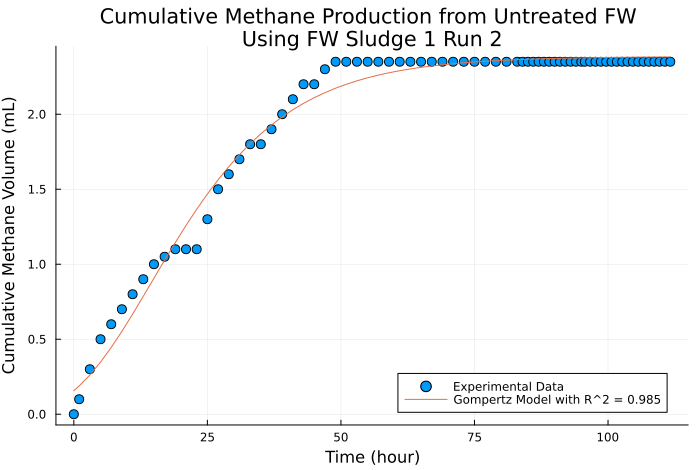
\includegraphics[width=.9\linewidth]{../plots/BMPs/Untreated FW/methane_kinetics_untreated_fw_s1_r2_hour.png}
\end{center}

\begin{center}
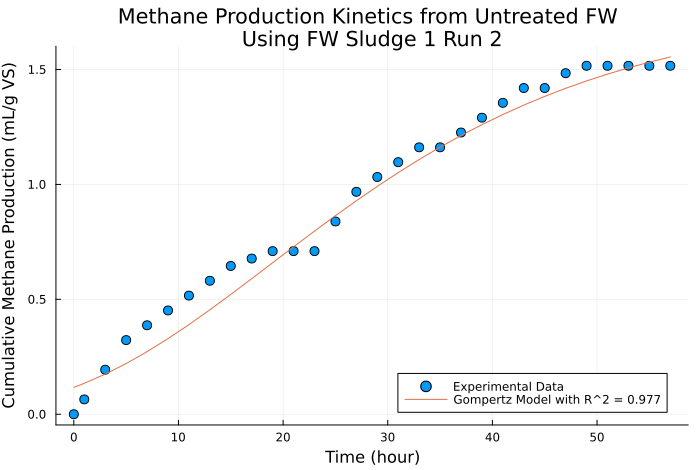
\includegraphics[width=.9\linewidth]{../plots/BMPs/Untreated FW/specific_methane_kinetics_untreated_fw_s1_r2_hour.png}
\end{center}

\subsection{Update all}
\label{sec:org837eb52}

\textbf{update\textsubscript{hydrolysate}\textsubscript{tests}\textsubscript{s1}\textsubscript{r2}}
\begin{minted}[breaklines=true,breakanywhere=true]{julia}

<<hydrolysate_0_s1_r2>>
<<hydrolysate_1_s1_r2>>
<<hydrolysate_2_s1_r2>>
<<hydrolysate_4_s1_r2>>
<<untreated_fw_s1_r2>>

model_fit_table_min = Tables.table(vcat(reshape(model_hydro_0_min, 1, 5), reshape(model_hydro_1_min, 1, 5), reshape(model_hydro_2_min, 1, 5), reshape(model_hydro_4_min, 1, 5), reshape(model_hydro_fw_min, 1, 5)), header = [:Reactor_Name, :Production_Potential, :Production_Rate, :Lag_Time, :R_squared])
CSV.write(datadir("exp_pro", "methane_from_hydrolysate_kinetics_min_s1_r2.csv"), model_fit_table_min)

model_fit_table_hour = Tables.table(vcat(reshape(model_hydro_0_hour, 1, 5), reshape(model_hydro_1_hour, 1, 5), reshape(model_hydro_2_hour, 1, 5), reshape(model_hydro_4_hour, 1, 5), reshape(model_hydro_fw_hour, 1, 5)), header = [:Reactor_Name, :Production_Potential, :Production_Rate, :Lag_Time, :R_squared])
CSV.write(datadir("exp_pro", "methane_from_hydrolysate_kinetics_hour_s1_r2.csv"), model_fit_table_hour)
return("../data/exp_pro/methane_from_hydrolysate_kinetics_min_s1_r2.csv")
\end{minted}

\begin{minted}[breaklines=true,breakanywhere=true]{julia}
return("../data/exp_pro/methane_from_hydrolysate_kinetics_hour_s1_r2.csv")
\end{minted}

\begin{minted}[breaklines=true,breakanywhere=true]{elisp}
(org-table-import-after-n-lines 4 <<hydrolysate_kinetic_name_hour_s1_r2()>> '(4))
\end{minted}

\begin{table}[htbp]
\caption{Kinetics with timescale in hours}
\centering
\begin{tabular}{lrrrr}
Reactor\textsubscript{Name} & Production\textsubscript{Potential} & Production\textsubscript{Rate} & Lag\textsubscript{Time} & R\textsubscript{squared}\\[0pt]
Reactor 0 & 3.726 & 0.044 & 3.854 & 0.992\\[0pt]
Reactor 1 & 10.568 & 0.107 & 4.425 & 0.996\\[0pt]
Reactor 2 & 7.912 & 0.115 & 0.0 & 0.923\\[0pt]
Reactor 4 & 8.294 & 0.08 & 0.348 & 0.988\\[0pt]
FW & 2.593 & 0.062 & 2.666 & 0.988\\[0pt]
\end{tabular}
\end{table}

\begin{minted}[breaklines=true,breakanywhere=true]{elisp}
(org-table-import-after-n-lines 4 <<update_hydrolysate_tests_s1_r2()>> '(4))
\end{minted}

\begin{table}[htbp]
\caption{Kinetics with timescale in minutes}
\centering
\begin{tabular}{lrrrr}
Reactor\textsubscript{Name} & Production\textsubscript{Potential} & Production\textsubscript{Rate} & Lag\textsubscript{Time} & R\textsubscript{squared}\\[0pt]
Reactor 0 & 3.7256 & 0.0007 & 231.2325 & 0.992\\[0pt]
Reactor 1 & 10.5683 & 0.0018 & 265.5173 & 0.996\\[0pt]
Reactor 2 & 7.7741 & 0.0021 & 0.0 & 0.929\\[0pt]
Reactor 4 & 8.2938 & 0.0013 & 20.8989 & 0.988\\[0pt]
FW & 2.5934 & 0.001 & 159.977 & 0.988\\[0pt]
\end{tabular}
\end{table}

\begin{minted}[breaklines=true,breakanywhere=true]{julia}

<<hydrolysate_0_s1_r2>>
<<hydrolysate_1_s1_r2>>
<<hydrolysate_2_s1_r2>>
<<hydrolysate_4_s1_r2>>
<<untreated_fw_s1_r2>>

sma_table = Tables.table(vcat(reshape(sma_hydro_0, 1, 5), reshape(sma_hydro_1, 1, 5), reshape(sma_hydro_2, 1, 5), reshape(sma_hydro_4, 1, 5), reshape(sma_hydro_fw, 1, 5)), header = [:Reactor_Name, :Methane_Potential, :SMA, :Lag_Time, :R_sq])
CSV.write(datadir("exp_pro", "sma_from_hydrolysate_s1_r2.csv"), sma_table)

return("../data/exp_pro/sma_from_hydrolysate_s1_r2.csv")
\end{minted}

\begin{minted}[breaklines=true,breakanywhere=true]{elisp}
(org-table-import-after-n-lines 4 <<sma_hydro_s1_r2()>> '(4))
\end{minted}

\begin{table}[htbp]
\caption{SMA Kinetics in hours}
\centering
\begin{tabular}{lrrrr}
Reactor\textsubscript{Name} & Methane\textsubscript{Potential} & SMA & Lag\textsubscript{Time} & R\textsubscript{sq}\\[0pt]
Reactor 0 & 2.404 & 0.028 & 3.854 & 0.992\\[0pt]
Reactor 1 & 7.046 & 0.071 & 4.425 & 0.996\\[0pt]
Reactor 2 & 5.105 & 0.074 & 0.0 & 0.923\\[0pt]
Reactor 4 & 5.351 & 0.052 & 0.348 & 0.988\\[0pt]
FW & 1.673 & 0.04 & 2.666 & 0.988\\[0pt]
\end{tabular}
\end{table}

\subsubsection{Σύγκριση με το προηγούμενο πείραμα}
\label{sec:org29434e2}
Γενικά, το 2ο πείραμα αυτό είναι συγκρίσιμο με το προηγούμενο, παρότι όχι ίδιο. Το πρώτο πείραμα έχει γενικά πιο γρήγορους ρυθμούς (κοντά σε 1.5 με 2 φορές αυτά). Επίσης, το πρώτο πείραμα έχει μηδενικό lag time σε όλα τα πειράματα, ενώ σε αυτό το πείραμα, 3 από τα 5 δείγματα είχαν κάποιο lag time και 2 από αυτά ήταν μάλιστα αρκετά σημαντικά.

Από άποψη παραγωγής μεθανίου, δεν υπάρχει κάποια ξεκάθαρη τάση. Σε κάποια δείγματα το ένα πείραμα παρήγαγε λίγο περισσότερο, σε κάποιες το άλλο. Αλλά, είναι γενικά κοντά, το οποίο είναι καλό.

\subsection{Plotting Methane Potential}
\label{sec:orge251311}
Σε αυτό το section θα γίνει ένα plot το οποίο θα συγκρίνει μέγιστο μεθάνιο (παραγωγή από οξικό) με αυτό που παράχθηκε από το FW. Θα γίνει με την ίδια λογική που έγινε και παραπάνω για το πρώτο run.

\begin{minted}[breaklines=true,breakanywhere=true]{julia}

<<update_acetate_tests_s1>>
<<update_hydrolysate_tests_s1_r2>>

comp_name = "s1_r2"
sludge = "Sludge 1 "
run = "Run 2"
<<BMP_comp_plot>>
\end{minted}

\begin{center}
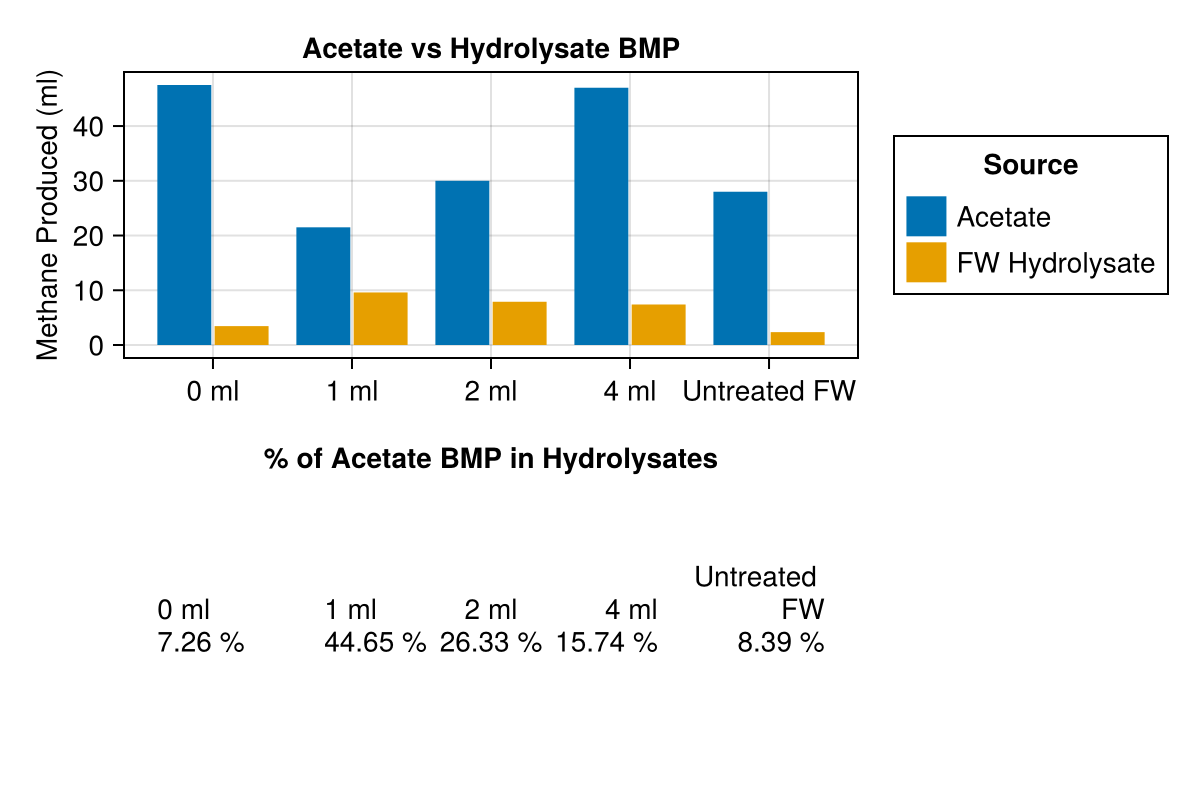
\includegraphics[width=.9\linewidth]{../plots/BMPs/Hydrolyzed FW/acet_vs_hydro_bmp_s1_r2.png}
\end{center}

\subsubsection{Σύγκριση με τον προηγούμενο κύκλο}
\label{sec:org622e2af}
Παρατηρούμε πως τα αποτελέσματα του πειράματος αυτού είναι αρκετά κοντά σε αυτά του προηγούμενου που δείχνει πως υπάρχει μία επαναληψιμότητα. Ακολουθείται η ίδια ακριβώς τάση 1 > 2 > 4 στα 3 πρώτα, ενώ το FW με το 0 έχουν εναλλαγεί στο πείραμα αυτό (βέβαια, έχουν και τα δύο πολύ χαμηλά αποτελέσματα οπότε μεταξύ τους σύγκριση δεν μας πειράζει). Βλέπουμε πως με μία εξαίρεση, οι αποκλίσεις είναι της τάξης του \(3 \%\) και ακόμη και εκείνη είναι \(6 \%\) το οποίο είναι σχετικά καλό. 

\subsection{Kinetic Comparison}
\label{sec:org3b6b92f}
\begin{minted}[breaklines=true,breakanywhere=true]{julia}

<<update_acetate_tests_s1>>
<<update_hydrolysate_tests_s1_r2>>

sludge = "s1"
run = "r2"
timescale = "hour"

<<ad_kinetics_comparison>>
return("../data/exp_pro/kinetics_comparison_s1_r2.csv")
\end{minted}

\begin{minted}[breaklines=true,breakanywhere=true]{julia}

<<update_acetate_tests_s1>>
<<update_hydrolysate_tests_s1_r2>>

sludge = "s1"
run = "r2"

<<manual_rate_comparison>>
return("../data/exp_pro/manual_max_rate_comp_s1_r2.csv")

\end{minted}

\begin{minted}[breaklines=true,breakanywhere=true]{julia}
return("../data/exp_pro/kinetics_comparison_sma_s1_r2.csv")
\end{minted}

\begin{minted}[breaklines=true,breakanywhere=true]{elisp}
(org-table-import-after-n-lines 4 <<kinetics_comp_s1_r2()>> '(4))
\end{minted}

\begin{table}[htbp]
\caption{Kinetic Comparison with timescale in hours}
\centering
\begin{tabular}{lrrr}
Reactor\textsubscript{Name} & Acetate & Hydrolysate & Ratio\\[0pt]
Reactor 0 & 459.84 & 0.044 & 0.0096\\[0pt]
Reactor 1 & 326.88 & 0.107 & 0.0327\\[0pt]
Reactor 2 & 374.04 & 0.113 & 0.0302\\[0pt]
Reactor 4 & 579.0 & 0.08 & 0.0138\\[0pt]
Reactor FW & 294.06 & 0.06 & 0.0204\\[0pt]
\end{tabular}
\end{table}

\begin{minted}[breaklines=true,breakanywhere=true]{elisp}
(org-table-import-after-n-lines 4 <<sma_comp_s1_r2()>> '(4))
\end{minted}

\begin{table}[htbp]
\caption{SMA Comparison with timescale in days}
\centering
\begin{tabular}{lrrr}
Reactor\textsubscript{Name} & Acetate & Hydrolysate & Ratio\\[0pt]
Reactor 0 & 7119.36 & 0.672 & 0.0094\\[0pt]
Reactor 1 & 5061.6 & 1.704 & 0.0337\\[0pt]
Reactor 2 & 5676.48 & 1.752 & 0.0309\\[0pt]
Reactor 4 & 8965.44 & 1.248 & 0.0139\\[0pt]
Reactor FW & 4554.72 & 0.936 & 0.0206\\[0pt]
\end{tabular}
\end{table}

\begin{minted}[breaklines=true,breakanywhere=true]{elisp}
(org-table-import-after-n-lines 3 <<manual_rates_s1_r2()>> '(4))
\end{minted}

\begin{center}
\begin{tabular}{lrrr}
Reactor & Acetate & Hydrolysate & Ratio\\[0pt]
Reactor 0 & 1025.641 & 0.1 & 0.01\\[0pt]
Reactor 1 & 643.564 & 6.024 & 0.936\\[0pt]
Reactor 2 & 555.556 & 6.173 & 1.111\\[0pt]
Reactor 4 & 1081.081 & 0.15 & 0.014\\[0pt]
Reactor FW & 705.882 & 0.1 & 0.014\\[0pt]
\end{tabular}
\end{center}

\subsection{Plotting Comparison Plots}
\label{sec:orgbd9a328}
Όπως και στον προηγούμενο κύκλο, φτιάχνουμε αυτό το χρήσιμο διάγραμμα.

\begin{minted}[breaklines=true,breakanywhere=true]{julia}

colors = ["#009AFA","#E36F47","#3EA44E","#C371D2","#AC8E18"]

<<hydrolysate_0_s1_r2>>
methane_s1_r2_comp = scatter(exp_hour, cumsum(exp_meth_vol), markersize = 4, legend = :outerright, label = "Hydrolysate (0 ml mix) Exp", xlabel = "Time (hour)", ylabel = "Cumulative Methane Volume (mL)", markercolor = colors[1], size = (1000, 600), legendfontsize = 12, labelfontsize = 14, tickfontsize = 12, left_margin=3Plots.mm,  bottom_margin=3Plots.mm, yticks = 0:2:10)
plot!(exp_hour, gompertz_bmp(exp_hour, model_hydro_0_hour[2:4]), label = "Hydrolysate (0 ml mix) Theoretical\n with "*L"R^2 = "*string(model_hydro_0_hour[5]), linecolor = colors[1])

<<hydrolysate_1_s1_r2>>
scatter!(methane_s1_r2_comp, exp_hour, cumsum(exp_meth_vol), markersize = 4, label = "Hydrolysate (1 ml mix) Exp", markercolor = colors[2])
plot!(exp_hour, gompertz_bmp(exp_hour, model_hydro_1_hour[2:4]), label = "Hydrolysate (1 ml mix) Theoretical\n with "*L"R^2 = "*string(model_hydro_1_hour[5]), linecolor = colors[2])

<<hydrolysate_2_s1_r2>>
scatter!(methane_s1_r2_comp, exp_hour, cumsum(exp_meth_vol), markersize = 4, label = "Hydrolysate (2 ml mix) Exp", markercolor = colors[3])
plot!(exp_hour, gompertz_bmp(exp_hour, model_hydro_2_hour[2:4]), label = "Hydrolysate (2 ml mix) Theoretical\n with "*L"R^2 = "*string(model_hydro_2_hour[5]), linecolor = colors[3])

<<hydrolysate_4_s1_r2>>
scatter!(methane_s1_r2_comp, exp_hour, cumsum(exp_meth_vol), markersize = 4, label = "Hydrolysate (4 ml mix) Exp", markercolor = colors[4])
plot!(exp_hour, gompertz_bmp(exp_hour, model_hydro_4_hour[2:4]), label = "Hydrolysate (4 ml mix) Theoretical\n with "*L"R^2 = "*string(model_hydro_4_hour[5]), linecolor = colors[4])

<<untreated_fw_s1_r2>>
scatter!(methane_s1_r2_comp, exp_hour, cumsum(exp_meth_vol), markersize = 4, label = "Untreated FW Exp", markercolor = colors[5])
plot!(exp_hour, gompertz_bmp(exp_hour, model_hydro_fw_hour[2:4]), label = "Untreated FW Theoretical\n with "*L"R^2 = "*string(model_hydro_fw_hour[5]), linecolor = colors[5])

savefig(methane_s1_r2_comp, plotsdir("BMPs", "methane_s1_r2_comp.svg"))
\end{minted}

\begin{center}
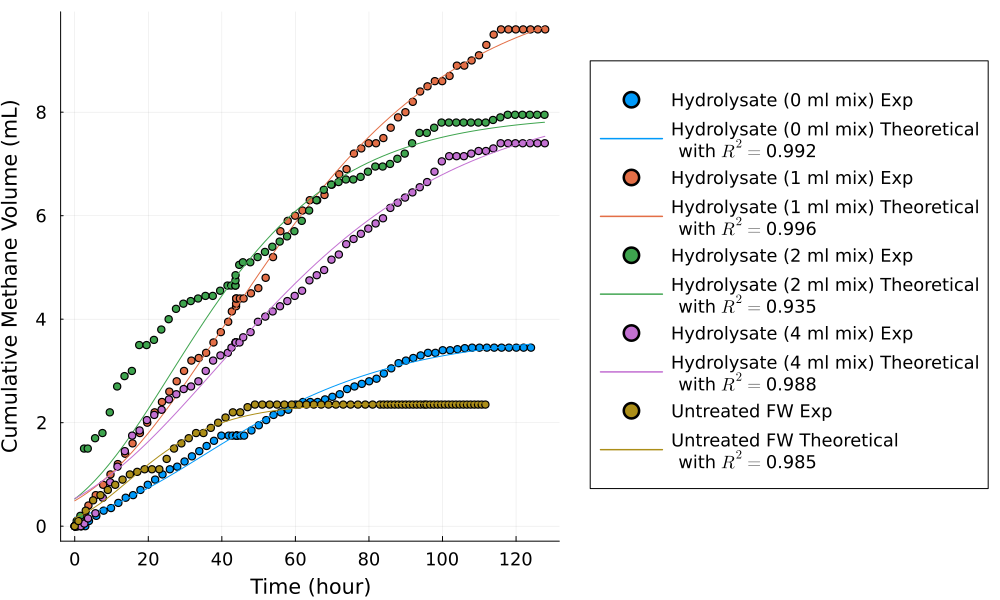
\includegraphics[width=.9\linewidth]{../plots/BMPs/methane_s1_r2_comp.png}
\end{center}

\subsection{Συμπεράσματα από τον κύκλο πειραμάτων αυτών}
\label{sec:orgecb442e}
Ο κύκλος αυτός ήταν αρκετά χρήσιμος επειδή μας έδειξε πως τα προηγούμενα αποτελέσματα έχουν σχετικά καλή επαναληψιμότητα καθώς και στους ρυθμούς αλλά και στην τελική παραγωγή μεθανίου, οι δύο κύκλοι είχαν παρόμοια αποτελέσματα. Το πείραμα δεν είναι τέλεια επαναλήψιμο, αλλά υπάρχουν αρκετές ομοιότητες.

Το μοντέλο Gompertz μπορεί να χρησιμοποιηθεί αποτελεσματικά για την κινητική ανάλυση της αναερόβιας χώνευσης καθώς έχει πολύ καλή προσαρμογή στα πειράματα και προβλέπει όλες τις φάσεις της μικροβιακής ανάπτυξης. Βέβαια, σε πολλές περιπτώσεις, παρόλο που το μοντέλο μπορεί να προβλέψει μία στάσιμη φάση, η διάρκεια της βγάινει ίση με 0, το οποίο σημαίνει πως η λάσπη αντιδρά πολύ γρήγορα στην προσθήκη του υποστρώματος αυτού. Πιθανή αιτία είναι πως όλα τα υποστρώματα έχουν κάποια ποσότητα οξικού οξέος, το οποίο ως η ιδανική τροφή της λάσπης καταναλώνεται αμέσως.

Από την άποψη των BMPs, η σειρά είναι 0 > FW > 4 > 2 > 1 (ίδια σειρά με πριν με εξαίρεση την αλλαγή του FW με το 0). Το FW και το 0 είναι πάλι και τα 2 πολύ χαμηλά, το οποίο κάνει ξανά validate ότι η προεπεξεργασία που επιλέχθηκε είναι αρκετά αποτελεσματική Το δείγμα 1 έχει και πάλι την περισσότερη ποσότητα μεθανίου. Αυτό δεν μπορεί να αιτιολογηθεί εύκολα από τα αποτελέσματα του αρχικού πειράματος υδρόλυσης σε αυτές τις συνθήκες, αλλά η αναπάντεχα μεγάλη συγκέντρωση sCOD του, οδηγεί στο συμπέρασμα της καλύτερης διαλυτοποίησης σε αυτό το πείραμα και πιθανόν αυτό να ευθύνεται για την αυξημένη παραγωγή μεθανίου.

\subsection{Code Block για Tangling}
\label{sec:org4b4db4e}
Έχοντας κάνει όλη αυτήν την ανάλυση, κάνουμε tangle ένα συνολικό code block σε ένα julia script file για sharing. Λόγω του structure του αρχείου αυτού και το ότι βασίζεται αρκετά στο org babel και το noweb syntax, το script file θα έχει αναγκαστικά πολλές επαναλήψεις. Αλλά θα είναι perfectly usable σε άλλο υπολογιστή θεωρητικά.

\begin{minted}[breaklines=true,breakanywhere=true]{julia}

<<update_acetate_tests_s1>>

sma_table = Tables.table(vcat(reshape(sma_acet_0, 1, 5), reshape(sma_acet_1, 1, 5), reshape(sma_acet_2, 1, 5), reshape(sma_acet_4, 1, 5), reshape(sma_acet_fw, 1, 5)), header = [:Reactor_Name, :Methane_Potential, :SMA, :Lag_Time, :R_sq])
CSV.write(datadir("exp_pro", "sma_from_acetate_s1.csv"), sma_table)

<<update_hydrolysate_tests_s1_r2>>

sma_table = Tables.table(vcat(reshape(sma_hydro_0, 1, 5), reshape(sma_hydro_1, 1, 5), reshape(sma_hydro_2, 1, 5), reshape(sma_hydro_4, 1, 5), reshape(sma_hydro_fw, 1, 5)), header = [:Reactor_Name, :Methane_Potential, :SMA, :Lag_Time, :R_sq])
CSV.write(datadir("exp_pro", "sma_from_hydrolysate_s1_r2.csv"), sma_table)

comp_name = "s1_r2"
sludge = "Sludge 1 "
run = "Run 2"
<<BMP_comp_plot>>

sludge = "s1"
run = "r2"
timescale = "hour"

<<ad_kinetics_comparison>>
<<manual_rate_comparison>>
\end{minted}

\section{Acetate Experiment Processing S2}
\label{sec:orgb660b2f}
Παρακάτω αναφέρονται οι δοκιμές που έγιναν με 100 μL οξικό σε κάθε δείγμα και θα χρησιμοποιηθούν συγκριτικά σε σχέση με τα FW. Μετά από τα code blocks που τρέχουν τον κώδικα θα υπάρχουν και κάποια από τα corresponding αποτελέσματα. Συγκεκριμένα, ο πίνακας με τα κινητικά δεδομένα και το διάγραμμα παραγωγής μεθανίου το οποίο έχει το curve fitting. Υπάρχουν και κάποια άλλα χρήσιμα διαγράμματα, τα οποία είναι αποθηκευμένα, αλλά εδώ παρατίθενται κάποια για καλύτερη ανάγνωση του αρχείου.

Το section αυτό αφορά την χρήση της 2ης λάσπης. Κατά την χρήση αυτής, παρατηρήθηκε ένα περίεργο φαινόμενο, το οποίο επαναλήφθηκε και στα πειράματα αυτά με το οξικό, αλλά και στα επερχόμενα υδρολύματα. Η λάσπη συνέχιζε να παράγει μεθάνιο σε πολύ μεγάλες ποσότητες για πολύ μεγάλο χρόνο, ξεπερνώντας κατά πολύ την ποσότητα που θα αναμενόταν να παράγουν 100 mg COD. Επίσης, στο οξικό η συνέχεια της παραγωγής έγινε μετά από όταν είχε σταματήσει για περίπου μισή μέρα. Οπότε, έγινε η υπόθεση ότι η συνέχεια της παραγωγής ήταν από κάποια τροφή που είχε αποθηκευμένη η λάσπη και δεν οφειλόταν στην τροφοδοσία που κάναμε. Έτσι την θεωρήσαμε ένα negative blank του πειράματος και αφαιρέσαμε την παραγωγή αυτή από τα υδρολύματα για να βγούν πιο εύλογα συμπεράσματα.

\subsection{Acetate Test FW}
\label{sec:org4c3952a}
Το section αυτό αναφέρεται στη δοκιμή με 100 μL οξικό στο δείγμα labelled ως FW (στο οποίο θα τροφοδοτηθούν untreated FW). 

\textbf{acet\textsubscript{test}\textsubscript{fw}\textsubscript{s2}}
\begin{minted}[breaklines=true,breakanywhere=true]{julia}

### Data Analysis on Reactor FW ###

<<date_saving_acetate_s2>>

inds = 1:16
exp_meth_vol = [0, 1.0, 5.0, 3.0, 1.5, 2.0, 0.5, 1.0, 0.5, 0, 0, 0, 0, 0, 0, 0]
meth_vol_acet_fw = cumsum(exp_meth_vol)[end]
exp_name = "acet_test_fw_s2"
source = "Acetate"
reactor = "Reactor FW"
sludge = "Sludge 2"
run_num = "Run 1"
input_vs = 4.2

p0 = [25.0, 6.0, 1.0]
<<bmp_data_processing>>
max_rate_acet_fw = max_manual_rate

<<bmp_curve_fitting_min>>
model_acet_fw = vcat(reactor, round.(model_params, digits = 3), round(r_squared, digits = 3))
<<bmp_data_plotting>>

<<sma_curve_fitting_min>>
sma_acet_fw = vcat(reactor, round.(model_params, digits = 3), round(r_squared, digits = 3))  
<<bmp_data_plotting>>

return("../data/exp_pro/"*exp_name*".csv")
\end{minted}

\begin{minted}[breaklines=true,breakanywhere=true]{elisp}
(org-table-import-after-n-lines 4 <<acet_test_fw_s2()>> '(4))
\end{minted}

\begin{table}[htbp]
\caption{Κινητικά δεδομένα}
\centering
\begin{tabular}{lrrrr}
Timestamp & Seconds & Minutes & Methane\textsubscript{Volume} & Cumulative\textsubscript{Methane}\textsubscript{Volume}\\[0pt]
10/04\textsubscript{13}:59 & 0.0 & 0.0 & 0.0 & 0.0\\[0pt]
10/04\textsubscript{14}:00 & 53.787 & 0.8964 & 1.0 & 1.0\\[0pt]
10/04\textsubscript{14}:01 & 113.801 & 1.8967 & 5.0 & 6.0\\[0pt]
10/04\textsubscript{14}:02 & 151.446 & 2.5241 & 3.0 & 9.0\\[0pt]
10/04\textsubscript{14}:03 & 211.446 & 3.5241 & 1.5 & 10.5\\[0pt]
10/04\textsubscript{14}:04 & 259.738 & 4.329 & 2.0 & 12.5\\[0pt]
10/04\textsubscript{14}:05 & 317.119 & 5.2853 & 0.5 & 13.0\\[0pt]
10/04\textsubscript{14}:06 & 377.141 & 6.2857 & 1.0 & 14.0\\[0pt]
10/04\textsubscript{14}:07 & 437.131 & 7.2855 & 0.5 & 14.5\\[0pt]
10/04\textsubscript{14}:07 & 455.72 & 7.5953 & 0.0 & 14.5\\[0pt]
10/04\textsubscript{14}:08 & 515.711 & 8.5952 & 0.0 & 14.5\\[0pt]
10/04\textsubscript{14}:08 & 543.733 & 9.0622 & 0.0 & 14.5\\[0pt]
10/04\textsubscript{14}:09 & 603.728 & 10.0621 & 0.0 & 14.5\\[0pt]
10/04\textsubscript{14}:10 & 663.726 & 11.0621 & 0.0 & 14.5\\[0pt]
10/04\textsubscript{14}:11 & 723.748 & 12.0625 & 0.0 & 14.5\\[0pt]
10/04\textsubscript{14}:12 & 783.759 & 13.0626 & 0.0 & 14.5\\[0pt]
\end{tabular}
\end{table}

\begin{center}
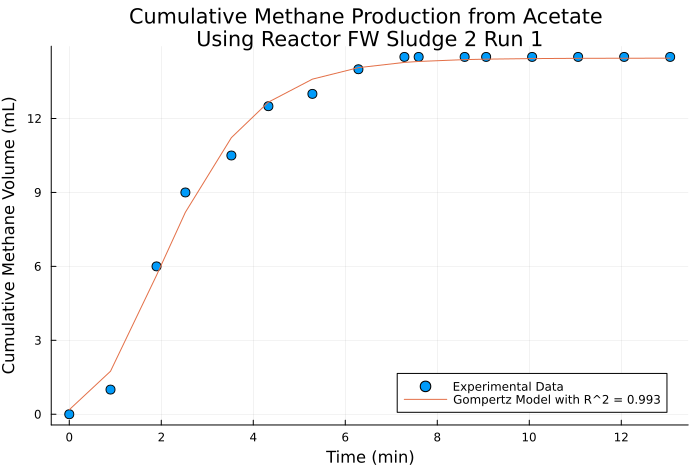
\includegraphics[width=.9\linewidth]{../plots/BMPs/Acetate/methane_kinetics_acet_test_fw_s2_min.png}
\end{center}

\begin{center}
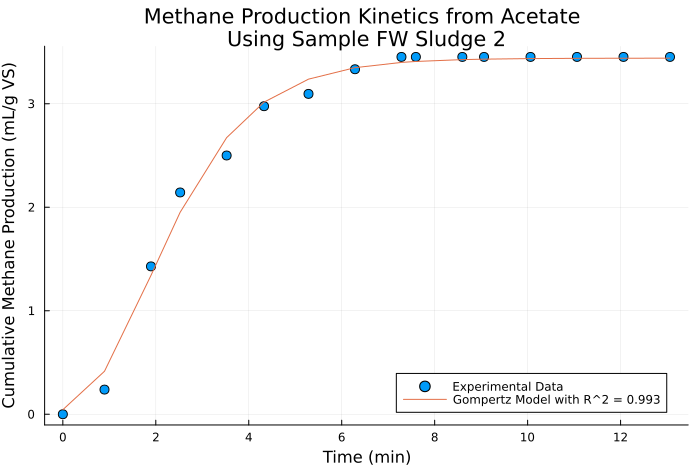
\includegraphics[width=.9\linewidth]{../plots/BMPs/Acetate/specific_methane_kinetics_acet_test_fw_s2.png}
\end{center}

\subsubsection{Continued}
\label{sec:org8b3ce0f}
Αυτό το section είναι για την συνέχεια του πειράματος, η οποία θα χρησιμοποιηθεί ως το negative blank για την ανάλυση των πειραμάτων με υδρόλυμα.

\begin{minted}[breaklines=true,breakanywhere=true]{julia}

<<date_saving_acetate_s2_2>>

inds = 33:110
exp_meth_vol = [1, 1, 0.5, 1, 1, 0.2, 0.5, 1, 0.5, 1, 0.5, 0.5, 1, 0.3, 1, 0.5, 0.5, 0.5, 0.5, 0.5, 1, 0.5, 1, 0.5, 1, 0.3, 1, 1, 0.3, 0.5, 1, 1, 0.5, 1, 0.5, 0.5, 1, 0.5, 0.5, 0.5, 0.5, 0.5, 1, 1, 0.5, 1, 1, 1, 1, 0.5, 0.5, 0.5, 0.5, 0.5, 0.5, 1, 0.5, 0.5, 1, 0.5, 1, 0.5, 0.5, 0.2, 0.2, 0.5, 0.5, 0.5, 0.5, 0.5, 0.5, 0.5, 0.5, 0.0, 0.0, 0, 0, 0]
meth_vol_acet_fw = cumsum(exp_meth_vol)[end]
exp_name = "acet_test_fw_s2_2"
source = "Acetate"
reactor = "Reactor FW"
sludge = "Sludge 2"
run_num = "Run 2"
input_vs = 4.2
pfw = [90.0, 20.0, 1.0]

<<bmp_data_processing>>
max_rate_acet_fw_2 = max_manual_rate

<<bmp_curve_fitting_hour>>
model_acet_fw = vcat(reactor, round.(model_params, digits = 3), round(r_squared, digits = 3))
<<bmp_data_plotting>>

<<sma_curve_fitting_hour>>
sma_acet_fw = vcat(reactor, round.(model_params, digits = 3), round(r_squared, digits = 3))  
<<bmp_data_plotting>>

return("../data/exp_pro/"*exp_name*".csv")

\end{minted}

\begin{minted}[breaklines=true,breakanywhere=true]{elisp}
(org-table-import-after-n-lines 3 <<acet_test_fw_s2_2()>> '(4))
\end{minted}

\begin{center}
\begin{tabular}{lrrrr}
Timestamp & Seconds & Minutes & Methane\textsubscript{Volume} & Cumulative\textsubscript{Methane}\textsubscript{Volume}\\[0pt]
12/04\textsubscript{05}:34 & 0.0 & 0.0 & 1.0 & 1.0\\[0pt]
12/04\textsubscript{06}:34 & 3600.007 & 60.0001 & 1.0 & 2.0\\[0pt]
12/04\textsubscript{07}:34 & 7200.239 & 120.004 & 0.5 & 2.5\\[0pt]
12/04\textsubscript{08}:34 & 10800.481 & 180.008 & 1.0 & 3.5\\[0pt]
12/04\textsubscript{09}:34 & 14400.548 & 240.0091 & 1.0 & 4.5\\[0pt]
12/04\textsubscript{10}:34 & 18000.58 & 300.0097 & 0.2 & 4.7\\[0pt]
12/04\textsubscript{11}:34 & 21600.582 & 360.0097 & 0.5 & 5.2\\[0pt]
12/04\textsubscript{12}:34 & 25200.581 & 420.0097 & 1.0 & 6.2\\[0pt]
12/04\textsubscript{13}:34 & 28800.579 & 480.0096 & 0.5 & 6.7\\[0pt]
12/04\textsubscript{14}:34 & 32400.584 & 540.0097 & 1.0 & 7.7\\[0pt]
12/04\textsubscript{15}:34 & 36000.582 & 600.0097 & 0.5 & 8.2\\[0pt]
12/04\textsubscript{16}:34 & 39600.955 & 660.0159 & 0.5 & 8.7\\[0pt]
12/04\textsubscript{17}:34 & 43201.278 & 720.0213 & 1.0 & 9.7\\[0pt]
12/04\textsubscript{18}:34 & 46801.285 & 780.0214 & 0.3 & 10.0\\[0pt]
12/04\textsubscript{19}:34 & 50401.282 & 840.0214 & 1.0 & 11.0\\[0pt]
12/04\textsubscript{20}:34 & 54001.29 & 900.0215 & 0.5 & 11.5\\[0pt]
12/04\textsubscript{21}:34 & 57601.287 & 960.0214 & 0.5 & 12.0\\[0pt]
12/04\textsubscript{22}:34 & 61201.293 & 1020.0216 & 0.5 & 12.5\\[0pt]
12/04\textsubscript{23}:34 & 64801.732 & 1080.0289 & 0.5 & 13.0\\[0pt]
13/04\textsubscript{00}:34 & 68401.73 & 1140.0288 & 0.5 & 13.5\\[0pt]
13/04\textsubscript{01}:34 & 72001.733 & 1200.0289 & 1.0 & 14.5\\[0pt]
13/04\textsubscript{02}:34 & 75601.752 & 1260.0292 & 0.5 & 15.0\\[0pt]
13/04\textsubscript{03}:34 & 79201.753 & 1320.0292 & 1.0 & 16.0\\[0pt]
13/04\textsubscript{04}:34 & 82801.759 & 1380.0293 & 0.5 & 16.5\\[0pt]
13/04\textsubscript{05}:34 & 86401.748 & 1440.0291 & 1.0 & 17.5\\[0pt]
13/04\textsubscript{06}:34 & 90001.754 & 1500.0292 & 0.3 & 17.8\\[0pt]
13/04\textsubscript{07}:34 & 93601.751 & 1560.0292 & 1.0 & 18.8\\[0pt]
13/04\textsubscript{08}:34 & 97201.748 & 1620.0291 & 1.0 & 19.8\\[0pt]
13/04\textsubscript{09}:34 & 100801.755 & 1680.0292 & 0.3 & 20.1\\[0pt]
13/04\textsubscript{10}:34 & 104402.092 & 1740.0349 & 0.5 & 20.6\\[0pt]
13/04\textsubscript{11}:34 & 108002.497 & 1800.0416 & 1.0 & 21.6\\[0pt]
13/04\textsubscript{12}:34 & 111602.598 & 1860.0433 & 1.0 & 22.6\\[0pt]
13/04\textsubscript{13}:34 & 115202.679 & 1920.0446 & 0.5 & 23.1\\[0pt]
13/04\textsubscript{14}:34 & 118802.729 & 1980.0455 & 1.0 & 24.1\\[0pt]
13/04\textsubscript{15}:34 & 122402.759 & 2040.046 & 0.5 & 24.6\\[0pt]
13/04\textsubscript{16}:34 & 126002.811 & 2100.0468 & 0.5 & 25.1\\[0pt]
13/04\textsubscript{17}:34 & 129603.047 & 2160.0508 & 1.0 & 26.1\\[0pt]
13/04\textsubscript{18}:34 & 133203.054 & 2220.0509 & 0.5 & 26.6\\[0pt]
13/04\textsubscript{19}:34 & 136803.062 & 2280.051 & 0.5 & 27.1\\[0pt]
13/04\textsubscript{20}:34 & 140403.155 & 2340.0526 & 0.5 & 27.6\\[0pt]
13/04\textsubscript{21}:34 & 144003.167 & 2400.0528 & 0.5 & 28.1\\[0pt]
13/04\textsubscript{22}:34 & 147603.184 & 2460.0531 & 0.5 & 28.6\\[0pt]
13/04\textsubscript{23}:34 & 151203.182 & 2520.053 & 1.0 & 29.6\\[0pt]
14/04\textsubscript{00}:34 & 154803.189 & 2580.0532 & 1.0 & 30.6\\[0pt]
14/04\textsubscript{01}:34 & 158403.186 & 2640.0531 & 0.5 & 31.1\\[0pt]
14/04\textsubscript{02}:34 & 162003.183 & 2700.053 & 1.0 & 32.1\\[0pt]
14/04\textsubscript{03}:34 & 165603.191 & 2760.0532 & 1.0 & 33.1\\[0pt]
14/04\textsubscript{04}:34 & 169203.37 & 2820.0562 & 1.0 & 34.1\\[0pt]
14/04\textsubscript{05}:34 & 172803.733 & 2880.0622 & 1.0 & 35.1\\[0pt]
14/04\textsubscript{06}:34 & 176403.88 & 2940.0647 & 0.5 & 35.6\\[0pt]
14/04\textsubscript{07}:34 & 180003.931 & 3000.0655 & 0.5 & 36.1\\[0pt]
14/04\textsubscript{08}:34 & 183603.985 & 3060.0664 & 0.5 & 36.6\\[0pt]
14/04\textsubscript{09}:34 & 187204.02 & 3120.067 & 0.5 & 37.1\\[0pt]
14/04\textsubscript{10}:34 & 190804.062 & 3180.0677 & 0.5 & 37.6\\[0pt]
14/04\textsubscript{11}:34 & 194404.095 & 3240.0682 & 0.5 & 38.1\\[0pt]
14/04\textsubscript{12}:34 & 198004.537 & 3300.0756 & 1.0 & 39.1\\[0pt]
14/04\textsubscript{13}:34 & 201604.565 & 3360.0761 & 0.5 & 39.6\\[0pt]
14/04\textsubscript{14}:34 & 205204.543 & 3420.0757 & 0.5 & 40.1\\[0pt]
14/04\textsubscript{15}:34 & 208804.542 & 3480.0757 & 1.0 & 41.1\\[0pt]
14/04\textsubscript{16}:34 & 212404.571 & 3540.0762 & 0.5 & 41.6\\[0pt]
14/04\textsubscript{17}:34 & 216004.759 & 3600.0793 & 1.0 & 42.6\\[0pt]
14/04\textsubscript{18}:34 & 219604.756 & 3660.0793 & 0.5 & 43.1\\[0pt]
14/04\textsubscript{19}:34 & 223204.837 & 3720.0806 & 0.5 & 43.6\\[0pt]
14/04\textsubscript{20}:34 & 226804.77 & 3780.0795 & 0.2 & 43.8\\[0pt]
14/04\textsubscript{21}:34 & 230404.765 & 3840.0794 & 0.2 & 44.0\\[0pt]
14/04\textsubscript{22}:34 & 234004.764 & 3900.0794 & 0.5 & 44.5\\[0pt]
14/04\textsubscript{23}:34 & 237605.363 & 3960.0894 & 0.5 & 45.0\\[0pt]
15/04\textsubscript{00}:34 & 241205.465 & 4020.0911 & 0.5 & 45.5\\[0pt]
15/04\textsubscript{01}:34 & 244805.506 & 4080.0918 & 0.5 & 46.0\\[0pt]
15/04\textsubscript{02}:34 & 248405.507 & 4140.0918 & 0.5 & 46.5\\[0pt]
15/04\textsubscript{03}:34 & 252005.516 & 4200.0919 & 0.5 & 47.0\\[0pt]
15/04\textsubscript{04}:34 & 255605.512 & 4260.0919 & 0.5 & 47.5\\[0pt]
15/04\textsubscript{05}:34 & 259205.523 & 4320.092 & 0.5 & 48.0\\[0pt]
15/04\textsubscript{06}:34 & 262805.519 & 4380.092 & 0.0 & 48.0\\[0pt]
15/04\textsubscript{07}:34 & 266405.514 & 4440.0919 & 0.0 & 48.0\\[0pt]
15/04\textsubscript{08}:34 & 270005.728 & 4500.0955 & 0.0 & 48.0\\[0pt]
15/04\textsubscript{09}:34 & 273605.803 & 4560.0967 & 0.0 & 48.0\\[0pt]
15/04\textsubscript{10}:34 & 277205.845 & 4620.0974 & 0.0 & 48.0\\[0pt]
\end{tabular}
\end{center}

\begin{center}
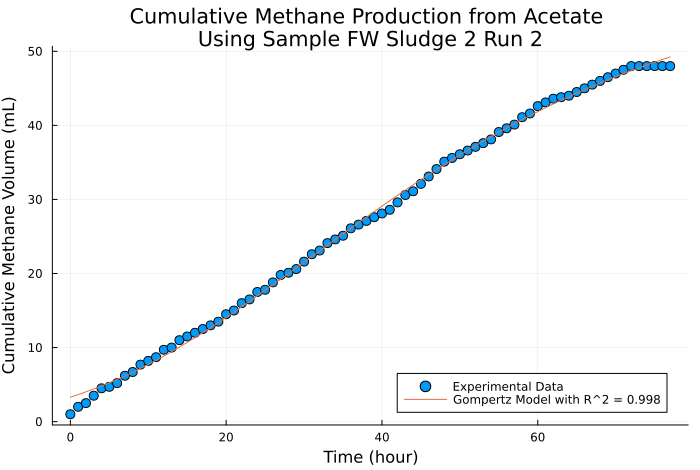
\includegraphics[width=.9\linewidth]{../plots/BMPs/Acetate/methane_kinetics_acet_test_fw_s2_2_hour.png}
\end{center}

\begin{center}
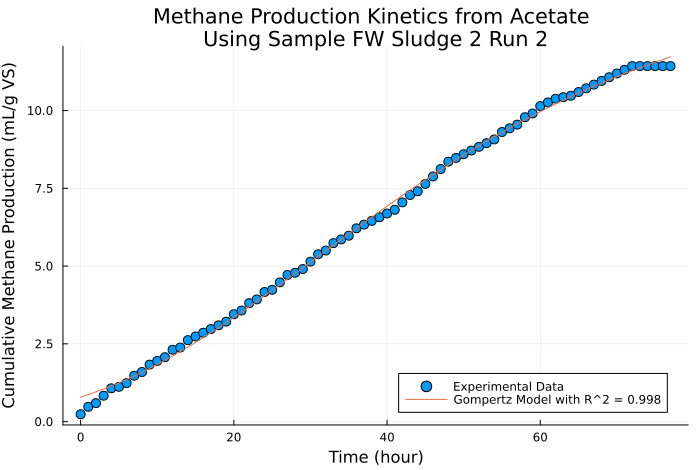
\includegraphics[width=.9\linewidth]{../plots/BMPs/Acetate/specific_methane_kinetics_acet_test_fw_s2_2_hour.png}
\end{center}

\subsection{Acetate Test 0}
\label{sec:org07a0bc8}
Το section αυτό αναφέρεται στη δοκιμή με 100 μL οξικό στο δείγμα (0).

\textbf{acet\textsubscript{test}\textsubscript{0}\textsubscript{s2}}
\begin{minted}[breaklines=true,breakanywhere=true]{julia}

### Data Analysis on Reactor 0 ###

<<date_saving_acetate_s2>>

inds = 12:21
exp_meth_vol = [0, 5.5, 1.0, 0.5, 0, 0, 0, 0, 0, 0]
meth_vol_acet_0 = cumsum(exp_meth_vol)[end]
exp_name = "acet_test_0_s2"
source = "Acetate"
reactor = "Reactor 0"
sludge = "Sludge 2"
run_num = "Run 1"
input_cod = 4.2
p0 = [40.0, 8.0, 1.0]

<<bmp_data_processing>>
max_rate_acet_0 = max_manual_rate

<<bmp_curve_fitting_min>>
model_acet_0 = vcat(reactor, round.(model_params, digits = 3), round(r_squared, digits = 3))
<<bmp_data_plotting>>

<<sma_curve_fitting_min>>
sma_acet_0 = vcat(reactor, round.(model_params, digits = 3), round(r_squared, digits = 3))  
<<bmp_data_plotting>>

return("../data/exp_pro/"*exp_name*".csv")
\end{minted}

\begin{minted}[breaklines=true,breakanywhere=true]{elisp}
(org-table-import-after-n-lines 4 <<acet_test_0_s2()>> '(4))
\end{minted}

\begin{table}[htbp]
\caption{Κινητικά δεδομένα}
\centering
\begin{tabular}{lrrrr}
Timestamp & Seconds & Minutes & Methane\textsubscript{Volume} & Cumulative\textsubscript{Methane}\textsubscript{Volume}\\[0pt]
10/04\textsubscript{14}:08 & 0.0 & 0.0 & 0.0 & 0.0\\[0pt]
10/04\textsubscript{14}:09 & 59.995 & 0.9999 & 5.5 & 5.5\\[0pt]
10/04\textsubscript{14}:10 & 119.993 & 1.9999 & 1.0 & 6.5\\[0pt]
10/04\textsubscript{14}:11 & 180.015 & 3.0002 & 0.5 & 7.0\\[0pt]
10/04\textsubscript{14}:12 & 240.026 & 4.0004 & 0.0 & 7.0\\[0pt]
10/04\textsubscript{14}:13 & 300.038 & 5.0006 & 0.0 & 7.0\\[0pt]
10/04\textsubscript{14}:14 & 360.043 & 6.0007 & 0.0 & 7.0\\[0pt]
10/04\textsubscript{14}:15 & 420.041 & 7.0007 & 0.0 & 7.0\\[0pt]
10/04\textsubscript{14}:16 & 480.031 & 8.0005 & 0.0 & 7.0\\[0pt]
10/04\textsubscript{14}:17 & 540.042 & 9.0007 & 0.0 & 7.0\\[0pt]
\end{tabular}
\end{table}

\begin{center}
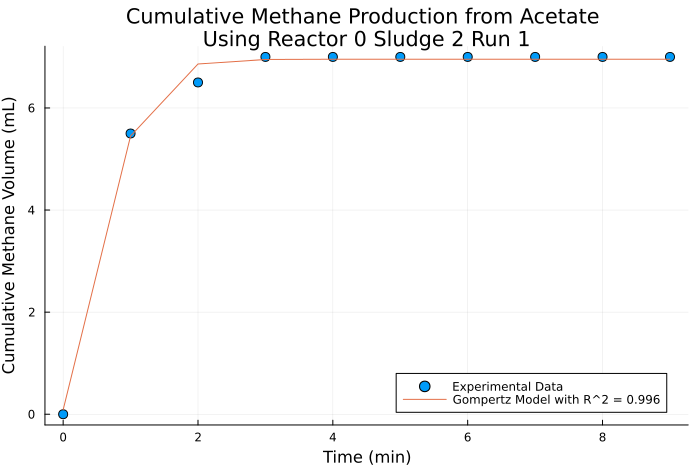
\includegraphics[width=.9\linewidth]{../plots/BMPs/Acetate/methane_kinetics_acet_test_0_s2_min.png}
\end{center}

\begin{center}
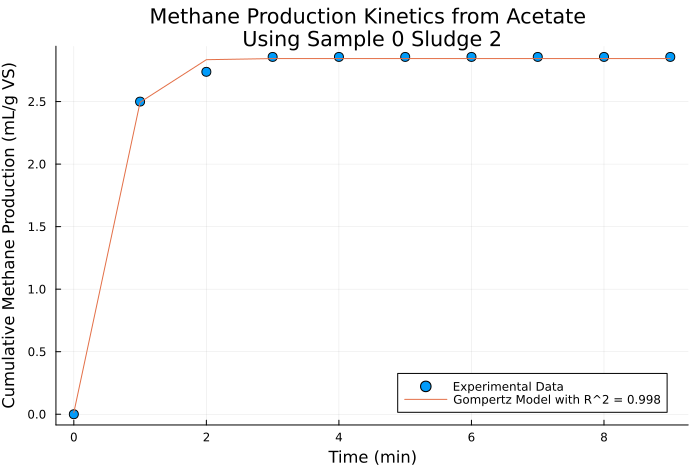
\includegraphics[width=.9\linewidth]{../plots/BMPs/Acetate/specific_methane_kinetics_acet_test_0_s2.png}
\end{center}

\subsubsection{Continued}
\label{sec:org056a37d}
Αυτό το section είναι για την συνέχεια του πειράματος, η οποία θα χρησιμοποιηθεί ως το negative blank για την ανάλυση των πειραμάτων με υδρόλυμα.

\begin{minted}[breaklines=true,breakanywhere=true]{julia}

<<date_saving_acetate_s2_2>>

inds = 7:104
exp_meth_vol = [0.5, 0.5, 0.5, 0.5, 1, 1, 1.5, 0.5, 0.5, 0.5, 1, 1, 1, 0.5, 0.5, 0.5, 0.5, 0.5, 0.5, 1, 1, 1, 1, 1, 1, 1, 1, 1, 0.5, 0.5, 0.5, 0.2, 0.2, 0.5, 0.5, 1, 1, 1, 0.5, 0.5, 0.5, 0.5, 0.5, 1, 0.5, 0.5, 0.5, 0.5, 0.5, 0.5, 0.5, 0.5, 0.5, 0.5, 0.5, 1, 1, 1, 1, 1, 0.5, 1, 1, 0.5, 0.5, 0.5, 1, 1, 0.5, 1, 0.5, 1, 0.5, 0.5, 1, 0.5, 0.5, 0.5, 1, 0.5, 0.5, 0.5, 0.5, 0.5, 1, 1, 1, 0.5, 0.5, 0.5, 0.5, 0.5, 0, 0, 0, 0, 0, 0]
meth_vol_acet_0 = cumsum(exp_meth_vol)[end]
exp_name = "acet_test_0_s2_2"
source = "Acetate"
reactor = "Reactor 0"
sludge = "Sludge 2"
run_num = "Run 2"
input_vs = 4.2
p0 = [90.0, 20.0, 1.0]

<<bmp_data_processing>>
max_rate_acet_0_2 = max_manual_rate

<<bmp_curve_fitting_hour>>
model_acet_0 = vcat(reactor, round.(model_params, digits = 3), round(r_squared, digits = 3))
<<bmp_data_plotting>>

<<sma_curve_fitting_hour>>
sma_acet_0 = vcat(reactor, round.(model_params, digits = 3), round(r_squared, digits = 3))  
<<bmp_data_plotting>>

return("../data/exp_pro/"*exp_name*".csv")

\end{minted}

\begin{minted}[breaklines=true,breakanywhere=true]{elisp}
(org-table-import-after-n-lines 3 <<acet_test_0_s2_2()>> '(4))
\end{minted}

\begin{center}
\begin{tabular}{lrrrr}
Timestamp & Seconds & Minutes & Methane\textsubscript{Volume} & Cumulative\textsubscript{Methane}\textsubscript{Volume}\\[0pt]
11/04\textsubscript{03}:34 & 0.0 & 0.0 & 0.5 & 0.5\\[0pt]
11/04\textsubscript{04}:34 & 3599.79 & 59.9965 & 0.5 & 1.0\\[0pt]
11/04\textsubscript{05}:34 & 7199.769 & 119.9962 & 0.5 & 1.5\\[0pt]
11/04\textsubscript{06}:34 & 10799.766 & 179.9961 & 0.5 & 2.0\\[0pt]
11/04\textsubscript{07}:34 & 14399.779 & 239.9963 & 1.0 & 3.0\\[0pt]
11/04\textsubscript{08}:34 & 17999.808 & 299.9968 & 1.0 & 4.0\\[0pt]
11/04\textsubscript{09}:34 & 21599.825 & 359.9971 & 1.5 & 5.5\\[0pt]
11/04\textsubscript{10}:34 & 25199.852 & 419.9975 & 0.5 & 6.0\\[0pt]
11/04\textsubscript{11}:34 & 28799.866 & 479.9978 & 0.5 & 6.5\\[0pt]
11/04\textsubscript{12}:34 & 32399.892 & 539.9982 & 0.5 & 7.0\\[0pt]
11/04\textsubscript{13}:34 & 36000.27 & 600.0045 & 1.0 & 8.0\\[0pt]
11/04\textsubscript{14}:34 & 39600.393 & 660.0065 & 1.0 & 9.0\\[0pt]
11/04\textsubscript{15}:34 & 43200.447 & 720.0074 & 1.0 & 10.0\\[0pt]
11/04\textsubscript{16}:34 & 46800.478 & 780.008 & 0.5 & 10.5\\[0pt]
11/04\textsubscript{17}:34 & 50401.576 & 840.0263 & 0.5 & 11.0\\[0pt]
11/04\textsubscript{18}:34 & 54001.607 & 900.0268 & 0.5 & 11.5\\[0pt]
11/04\textsubscript{19}:34 & 57601.647 & 960.0274 & 0.5 & 12.0\\[0pt]
11/04\textsubscript{20}:34 & 61201.666 & 1020.0278 & 0.5 & 12.5\\[0pt]
11/04\textsubscript{21}:34 & 64801.711 & 1080.0285 & 0.5 & 13.0\\[0pt]
11/04\textsubscript{22}:34 & 68401.258 & 1140.021 & 1.0 & 14.0\\[0pt]
11/04\textsubscript{23}:34 & 72001.106 & 1200.0184 & 1.0 & 15.0\\[0pt]
12/04\textsubscript{00}:34 & 75601.105 & 1260.0184 & 1.0 & 16.0\\[0pt]
12/04\textsubscript{01}:34 & 79201.13 & 1320.0188 & 1.0 & 17.0\\[0pt]
12/04\textsubscript{02}:34 & 82801.119 & 1380.0186 & 1.0 & 18.0\\[0pt]
12/04\textsubscript{03}:34 & 86401.125 & 1440.0188 & 1.0 & 19.0\\[0pt]
12/04\textsubscript{04}:34 & 90001.123 & 1500.0187 & 1.0 & 20.0\\[0pt]
12/04\textsubscript{05}:34 & 93601.118 & 1560.0186 & 1.0 & 21.0\\[0pt]
12/04\textsubscript{06}:34 & 97201.125 & 1620.0188 & 1.0 & 22.0\\[0pt]
12/04\textsubscript{07}:34 & 100801.357 & 1680.0226 & 0.5 & 22.5\\[0pt]
12/04\textsubscript{08}:34 & 104401.599 & 1740.0266 & 0.5 & 23.0\\[0pt]
12/04\textsubscript{09}:34 & 108001.666 & 1800.0278 & 0.5 & 23.5\\[0pt]
12/04\textsubscript{10}:34 & 111601.698 & 1860.0283 & 0.2 & 23.7\\[0pt]
12/04\textsubscript{11}:34 & 115201.7 & 1920.0283 & 0.2 & 23.9\\[0pt]
12/04\textsubscript{12}:34 & 118801.699 & 1980.0283 & 0.5 & 24.4\\[0pt]
12/04\textsubscript{13}:34 & 122401.697 & 2040.0283 & 0.5 & 24.9\\[0pt]
12/04\textsubscript{14}:34 & 126001.702 & 2100.0284 & 1.0 & 25.9\\[0pt]
12/04\textsubscript{15}:34 & 129601.7 & 2160.0283 & 1.0 & 26.9\\[0pt]
12/04\textsubscript{16}:34 & 133202.073 & 2220.0346 & 1.0 & 27.9\\[0pt]
12/04\textsubscript{17}:34 & 136802.396 & 2280.0399 & 0.5 & 28.4\\[0pt]
12/04\textsubscript{18}:34 & 140402.403 & 2340.04 & 0.5 & 28.9\\[0pt]
12/04\textsubscript{19}:34 & 144002.4 & 2400.04 & 0.5 & 29.4\\[0pt]
12/04\textsubscript{20}:34 & 147602.408 & 2460.0401 & 0.5 & 29.9\\[0pt]
12/04\textsubscript{21}:34 & 151202.405 & 2520.0401 & 0.5 & 30.4\\[0pt]
12/04\textsubscript{22}:34 & 154802.411 & 2580.0402 & 1.0 & 31.4\\[0pt]
12/04\textsubscript{23}:34 & 158402.85 & 2640.0475 & 0.5 & 31.9\\[0pt]
13/04\textsubscript{00}:34 & 162002.848 & 2700.0475 & 0.5 & 32.4\\[0pt]
13/04\textsubscript{01}:34 & 165602.851 & 2760.0475 & 0.5 & 32.9\\[0pt]
13/04\textsubscript{02}:34 & 169202.87 & 2820.0478 & 0.5 & 33.4\\[0pt]
13/04\textsubscript{03}:34 & 172802.871 & 2880.0478 & 0.5 & 33.9\\[0pt]
13/04\textsubscript{04}:34 & 176402.877 & 2940.048 & 0.5 & 34.4\\[0pt]
13/04\textsubscript{05}:34 & 180002.866 & 3000.0478 & 0.5 & 34.9\\[0pt]
13/04\textsubscript{06}:34 & 183602.872 & 3060.0479 & 0.5 & 35.4\\[0pt]
13/04\textsubscript{07}:34 & 187202.869 & 3120.0478 & 0.5 & 35.9\\[0pt]
13/04\textsubscript{08}:34 & 190802.866 & 3180.0478 & 0.5 & 36.4\\[0pt]
13/04\textsubscript{09}:34 & 194402.873 & 3240.0479 & 0.5 & 36.9\\[0pt]
13/04\textsubscript{10}:34 & 198003.21 & 3300.0535 & 1.0 & 37.9\\[0pt]
13/04\textsubscript{11}:34 & 201603.615 & 3360.0602 & 1.0 & 38.9\\[0pt]
13/04\textsubscript{12}:34 & 205203.716 & 3420.0619 & 1.0 & 39.9\\[0pt]
13/04\textsubscript{13}:34 & 208803.797 & 3480.0633 & 1.0 & 40.9\\[0pt]
13/04\textsubscript{14}:34 & 212403.847 & 3540.0641 & 1.0 & 41.9\\[0pt]
13/04\textsubscript{15}:34 & 216003.877 & 3600.0646 & 0.5 & 42.4\\[0pt]
13/04\textsubscript{16}:34 & 219603.929 & 3660.0655 & 1.0 & 43.4\\[0pt]
13/04\textsubscript{17}:34 & 223204.165 & 3720.0694 & 1.0 & 44.4\\[0pt]
13/04\textsubscript{18}:34 & 226804.172 & 3780.0695 & 0.5 & 44.9\\[0pt]
13/04\textsubscript{19}:34 & 230404.18 & 3840.0697 & 0.5 & 45.4\\[0pt]
13/04\textsubscript{20}:34 & 234004.273 & 3900.0712 & 0.5 & 45.9\\[0pt]
13/04\textsubscript{21}:34 & 237604.285 & 3960.0714 & 1.0 & 46.9\\[0pt]
13/04\textsubscript{22}:34 & 241204.302 & 4020.0717 & 1.0 & 47.9\\[0pt]
13/04\textsubscript{23}:34 & 244804.3 & 4080.0717 & 0.5 & 48.4\\[0pt]
14/04\textsubscript{00}:34 & 248404.307 & 4140.0718 & 1.0 & 49.4\\[0pt]
14/04\textsubscript{01}:34 & 252004.304 & 4200.0717 & 0.5 & 49.9\\[0pt]
14/04\textsubscript{02}:34 & 255604.301 & 4260.0717 & 1.0 & 50.9\\[0pt]
14/04\textsubscript{03}:34 & 259204.309 & 4320.0718 & 0.5 & 51.4\\[0pt]
14/04\textsubscript{04}:34 & 262804.488 & 4380.0748 & 0.5 & 51.9\\[0pt]
14/04\textsubscript{05}:34 & 266404.851 & 4440.0808 & 1.0 & 52.9\\[0pt]
14/04\textsubscript{06}:34 & 270004.998 & 4500.0833 & 0.5 & 53.4\\[0pt]
14/04\textsubscript{07}:34 & 273605.049 & 4560.0842 & 0.5 & 53.9\\[0pt]
14/04\textsubscript{08}:34 & 277205.103 & 4620.085 & 0.5 & 54.4\\[0pt]
14/04\textsubscript{09}:34 & 280805.138 & 4680.0856 & 1.0 & 55.4\\[0pt]
14/04\textsubscript{10}:34 & 284405.18 & 4740.0863 & 0.5 & 55.9\\[0pt]
14/04\textsubscript{11}:34 & 288005.213 & 4800.0869 & 0.5 & 56.4\\[0pt]
14/04\textsubscript{12}:34 & 291605.655 & 4860.0942 & 0.5 & 56.9\\[0pt]
14/04\textsubscript{13}:34 & 295205.683 & 4920.0947 & 0.5 & 57.4\\[0pt]
14/04\textsubscript{14}:34 & 298805.661 & 4980.0944 & 0.5 & 57.9\\[0pt]
14/04\textsubscript{15}:34 & 302405.66 & 5040.0943 & 1.0 & 58.9\\[0pt]
14/04\textsubscript{16}:34 & 306005.689 & 5100.0948 & 1.0 & 59.9\\[0pt]
14/04\textsubscript{17}:34 & 309605.877 & 5160.098 & 1.0 & 60.9\\[0pt]
14/04\textsubscript{18}:34 & 313205.874 & 5220.0979 & 0.5 & 61.4\\[0pt]
14/04\textsubscript{19}:34 & 316805.955 & 5280.0992 & 0.5 & 61.9\\[0pt]
14/04\textsubscript{20}:34 & 320405.888 & 5340.0981 & 0.5 & 62.4\\[0pt]
14/04\textsubscript{21}:34 & 324005.883 & 5400.098 & 0.5 & 62.9\\[0pt]
14/04\textsubscript{22}:34 & 327605.882 & 5460.098 & 0.5 & 63.4\\[0pt]
14/04\textsubscript{23}:34 & 331206.481 & 5520.108 & 0.0 & 63.4\\[0pt]
15/04\textsubscript{00}:34 & 334806.583 & 5580.1097 & 0.0 & 63.4\\[0pt]
15/04\textsubscript{01}:34 & 338406.624 & 5640.1104 & 0.0 & 63.4\\[0pt]
15/04\textsubscript{02}:34 & 342006.625 & 5700.1104 & 0.0 & 63.4\\[0pt]
15/04\textsubscript{03}:34 & 345606.634 & 5760.1106 & 0.0 & 63.4\\[0pt]
15/04\textsubscript{04}:34 & 349206.63 & 5820.1105 & 0.0 & 63.4\\[0pt]
\end{tabular}
\end{center}

\begin{center}
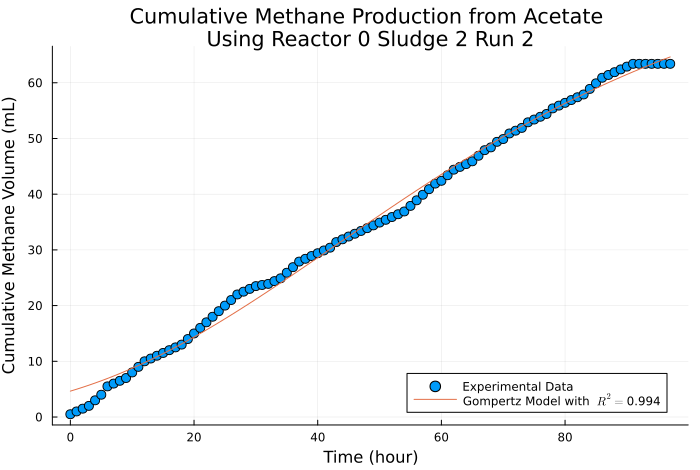
\includegraphics[width=.9\linewidth]{../plots/BMPs/Acetate/methane_kinetics_acet_test_0_s2_2_hour.png}
\end{center}

\begin{center}
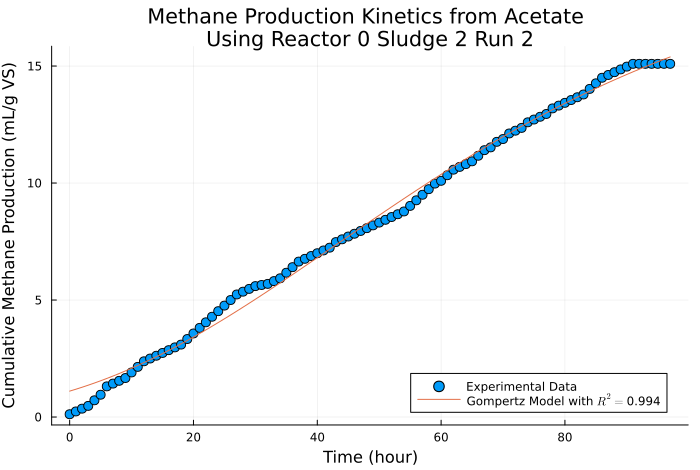
\includegraphics[width=.9\linewidth]{../plots/BMPs/Acetate/specific_methane_kinetics_acet_test_0_s2_2_hour.png}
\end{center}


\subsection{Acetate Test 1}
\label{sec:org1d6591c}
Το section αυτό αναφέρεται στη δοκιμή με 100 μL οξικό στο δείγμα (1). Aξίζει να αναφερθεί πως την πρώτη πειραματική ημέρα (27/03), παρήγαγε αέριο χωρίς να τροφοδοτηθεί με κάποιο υπόστρωμα. Η κινητική αυτής της παραγωγής (η οποία δεν ξέρουμε σε τι ευθύνεται) θα αναλυθεί παρακάτω. Βέβαια, μόλις τροφοδοτήθηκε με οξικό και η παραγωγή του τελείωσε, σταμάτησε και εκείνη η παραγωγή. Βέβαια, είχε την χαμηλότερη παραγωγή βιοαερίου μόλις τροφοδοτήθηκε με οξικό, οπότε ενδέχεται αυτή η μέτρηση να ήταν προβληματική.

\textbf{acet\textsubscript{test}\textsubscript{1}\textsubscript{s2}}
\begin{minted}[breaklines=true,breakanywhere=true]{julia}

### Data Analysis on Reactor 1 ###

<<date_saving_acetate_s2>>

inds = 7:21
exp_meth_vol = [0, 7, 2, 0.2, 0.8, 0.2, 1.5, 0, 0, 0, 0, 0, 0, 0, 0]
meth_vol_acet_1 = cumsum(exp_meth_vol)[end]
exp_name = "acet_test_1_s2"
source = "Acetate"
reactor = "Reactor 1"
sludge = "Sludge 2"
run_num = "Run 1"
input_vs = 4.2
p0 = [20.0, 4.0, 1.0]

<<bmp_data_processing>>
max_rate_acet_1 = max_manual_rate

<<bmp_curve_fitting_min>>
model_acet_1 = vcat(reactor, round.(model_params, digits = 3), round(r_squared, digits = 3))
<<bmp_data_plotting>>

<<sma_curve_fitting_min>>
sma_acet_1 = vcat(reactor, round.(model_params, digits = 3), round(r_squared, digits = 3))  
<<bmp_data_plotting>>

return("../data/exp_pro/"*exp_name*".csv")
\end{minted}

\begin{minted}[breaklines=true,breakanywhere=true]{elisp}
(org-table-import-after-n-lines 4 <<acet_test_1_s2()>> '(4))
\end{minted}

\begin{table}[htbp]
\caption{Κινητικά δεδομένα}
\centering
\begin{tabular}{lrrrr}
Timestamp & Seconds & Minutes & Methane\textsubscript{Volume} & Cumulative\textsubscript{Methane}\textsubscript{Volume}\\[0pt]
10/04\textsubscript{14}:05 & 0.0 & 0.0 & 0.0 & 0.0\\[0pt]
10/04\textsubscript{14}:06 & 60.022 & 1.0004 & 7.0 & 7.0\\[0pt]
10/04\textsubscript{14}:07 & 120.012 & 2.0002 & 2.0 & 9.0\\[0pt]
10/04\textsubscript{14}:07 & 138.601 & 2.31 & 0.2 & 9.2\\[0pt]
10/04\textsubscript{14}:08 & 198.592 & 3.3099 & 0.8 & 10.0\\[0pt]
10/04\textsubscript{14}:08 & 226.614 & 3.7769 & 0.2 & 10.2\\[0pt]
10/04\textsubscript{14}:09 & 286.609 & 4.7768 & 1.5 & 11.7\\[0pt]
10/04\textsubscript{14}:10 & 346.607 & 5.7768 & 0.0 & 11.7\\[0pt]
10/04\textsubscript{14}:11 & 406.629 & 6.7772 & 0.0 & 11.7\\[0pt]
10/04\textsubscript{14}:12 & 466.64 & 7.7773 & 0.0 & 11.7\\[0pt]
10/04\textsubscript{14}:13 & 526.652 & 8.7775 & 0.0 & 11.7\\[0pt]
10/04\textsubscript{14}:14 & 586.657 & 9.7776 & 0.0 & 11.7\\[0pt]
10/04\textsubscript{14}:15 & 646.655 & 10.7776 & 0.0 & 11.7\\[0pt]
10/04\textsubscript{14}:16 & 706.645 & 11.7774 & 0.0 & 11.7\\[0pt]
10/04\textsubscript{14}:17 & 766.656 & 12.7776 & 0.0 & 11.7\\[0pt]
\end{tabular}
\end{table}

\begin{center}
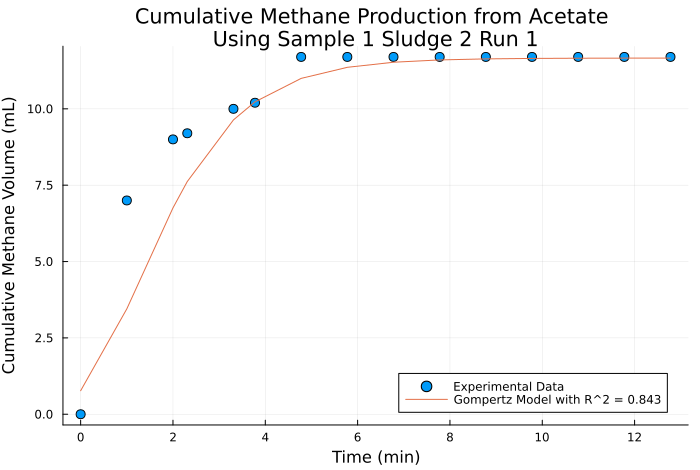
\includegraphics[width=.9\linewidth]{../plots/BMPs/Acetate/methane_kinetics_acet_test_1_s2_min.png}
\end{center}

\begin{center}
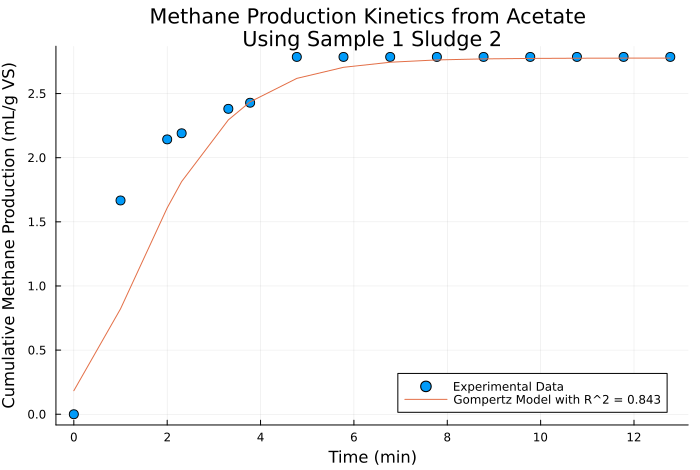
\includegraphics[width=.9\linewidth]{../plots/BMPs/Acetate/specific_methane_kinetics_acet_test_1_s2.png}
\end{center}

\subsubsection{Continued}
\label{sec:org15bf180}
Αυτό το section είναι για την συνέχεια του πειράματος, η οποία θα χρησιμοποιηθεί ως το negative blank για την ανάλυση των πειραμάτων με υδρόλυμα.

\begin{minted}[breaklines=true,breakanywhere=true]{julia}

<<date_saving_acetate_s2_2>>

inds = 2:75
exp_meth_vol = [0, 0.2, 1, 1.5, 1, 1, 1, 1, 1.5, 1.5, 1, 1, 1, 1, 1.5, 1.5, 1, 1, 1.5, 1, 1, 1, 1, 1, 1, 1, 1.5, 1, 1, 1, 1, 1, 1.5, 1.5, 1.5, 1.5, 1.5, 1.5, 1.5, 1, 1.5, 1.5, 1.5, 1.5, 1, 1, 1.5, 1.5, 1, 1, 1.5, 1, 1.5, 1, 1, 1, 1.5, 1, 1, 1, 1.5, 1, 1, 1, 1, 1, 1, 0, 0, 0, 0, 0, 0, 0]
meth_vol_acet_1 = cumsum(exp_meth_vol)[end]
exp_name = "acet_test_1_s2_2"
source = "Acetate"
reactor = "Reactor 1"
sludge = "Sludge 2"
run_num = "Run 2"
input_vs = 4.2
p0 = [90.0, 20.0, 1.0]

<<bmp_data_processing>>
max_rate_acet_1_2 = max_manual_rate

<<bmp_curve_fitting_hour>>
model_acet_1 = vcat(reactor, round.(model_params, digits = 3), round(r_squared, digits = 3))
<<bmp_data_plotting>>

<<sma_curve_fitting_hour>>
sma_acet_1 = vcat(reactor, round.(model_params, digits = 3), round(r_squared, digits = 3))  
<<bmp_data_plotting>>

return("../data/exp_pro/"*exp_name*".csv")

\end{minted}

\begin{minted}[breaklines=true,breakanywhere=true]{elisp}
(org-table-import-after-n-lines 3 <<acet_test_1_s2_2()>> '(4))
\end{minted}

\begin{center}
\begin{tabular}{lrrrr}
Timestamp & Seconds & Minutes & Methane\textsubscript{Volume} & Cumulative\textsubscript{Methane}\textsubscript{Volume}\\[0pt]
10/04\textsubscript{22}:34 & 0.0 & 0.0 & 0.0 & 0.0\\[0pt]
10/04\textsubscript{23}:34 & 3600.646 & 60.0108 & 0.2 & 0.2\\[0pt]
11/04\textsubscript{00}:34 & 7200.689 & 120.0115 & 1.0 & 1.2\\[0pt]
11/04\textsubscript{01}:34 & 10800.736 & 180.0123 & 1.5 & 2.7\\[0pt]
11/04\textsubscript{02}:34 & 14400.774 & 240.0129 & 1.0 & 3.7\\[0pt]
11/04\textsubscript{03}:34 & 18000.824 & 300.0137 & 1.0 & 4.7\\[0pt]
11/04\textsubscript{04}:34 & 21600.614 & 360.0102 & 1.0 & 5.7\\[0pt]
11/04\textsubscript{05}:34 & 25200.593 & 420.0099 & 1.0 & 6.7\\[0pt]
11/04\textsubscript{06}:34 & 28800.59 & 480.0098 & 1.5 & 8.2\\[0pt]
11/04\textsubscript{07}:34 & 32400.603 & 540.01 & 1.5 & 9.7\\[0pt]
11/04\textsubscript{08}:34 & 36000.632 & 600.0105 & 1.0 & 10.7\\[0pt]
11/04\textsubscript{09}:34 & 39600.649 & 660.0108 & 1.0 & 11.7\\[0pt]
11/04\textsubscript{10}:34 & 43200.676 & 720.0113 & 1.0 & 12.7\\[0pt]
11/04\textsubscript{11}:34 & 46800.69 & 780.0115 & 1.0 & 13.7\\[0pt]
11/04\textsubscript{12}:34 & 50400.716 & 840.0119 & 1.5 & 15.2\\[0pt]
11/04\textsubscript{13}:34 & 54001.094 & 900.0182 & 1.5 & 16.7\\[0pt]
11/04\textsubscript{14}:34 & 57601.217 & 960.0203 & 1.0 & 17.7\\[0pt]
11/04\textsubscript{15}:34 & 61201.271 & 1020.0212 & 1.0 & 18.7\\[0pt]
11/04\textsubscript{16}:34 & 64801.302 & 1080.0217 & 1.5 & 20.2\\[0pt]
11/04\textsubscript{17}:34 & 68402.4 & 1140.04 & 1.0 & 21.2\\[0pt]
11/04\textsubscript{18}:34 & 72002.431 & 1200.0405 & 1.0 & 22.2\\[0pt]
11/04\textsubscript{19}:34 & 75602.471 & 1260.0412 & 1.0 & 23.2\\[0pt]
11/04\textsubscript{20}:34 & 79202.49 & 1320.0415 & 1.0 & 24.2\\[0pt]
11/04\textsubscript{21}:34 & 82802.535 & 1380.0422 & 1.0 & 25.2\\[0pt]
11/04\textsubscript{22}:34 & 86402.082 & 1440.0347 & 1.0 & 26.2\\[0pt]
11/04\textsubscript{23}:34 & 90001.93 & 1500.0322 & 1.0 & 27.2\\[0pt]
12/04\textsubscript{00}:34 & 93601.929 & 1560.0322 & 1.5 & 28.7\\[0pt]
12/04\textsubscript{01}:34 & 97201.954 & 1620.0326 & 1.0 & 29.7\\[0pt]
12/04\textsubscript{02}:34 & 100801.943 & 1680.0324 & 1.0 & 30.7\\[0pt]
12/04\textsubscript{03}:34 & 104401.949 & 1740.0325 & 1.0 & 31.7\\[0pt]
12/04\textsubscript{04}:34 & 108001.947 & 1800.0324 & 1.0 & 32.7\\[0pt]
12/04\textsubscript{05}:34 & 111601.942 & 1860.0324 & 1.0 & 33.7\\[0pt]
12/04\textsubscript{06}:34 & 115201.949 & 1920.0325 & 1.5 & 35.2\\[0pt]
12/04\textsubscript{07}:34 & 118802.181 & 1980.0364 & 1.5 & 36.7\\[0pt]
12/04\textsubscript{08}:34 & 122402.423 & 2040.0404 & 1.5 & 38.2\\[0pt]
12/04\textsubscript{09}:34 & 126002.49 & 2100.0415 & 1.5 & 39.7\\[0pt]
12/04\textsubscript{10}:34 & 129602.522 & 2160.042 & 1.5 & 41.2\\[0pt]
12/04\textsubscript{11}:34 & 133202.524 & 2220.0421 & 1.5 & 42.7\\[0pt]
12/04\textsubscript{12}:34 & 136802.523 & 2280.042 & 1.5 & 44.2\\[0pt]
12/04\textsubscript{13}:34 & 140402.521 & 2340.042 & 1.0 & 45.2\\[0pt]
12/04\textsubscript{14}:34 & 144002.526 & 2400.0421 & 1.5 & 46.7\\[0pt]
12/04\textsubscript{15}:34 & 147602.524 & 2460.0421 & 1.5 & 48.2\\[0pt]
12/04\textsubscript{16}:34 & 151202.897 & 2520.0483 & 1.5 & 49.7\\[0pt]
12/04\textsubscript{17}:34 & 154803.22 & 2580.0537 & 1.5 & 51.2\\[0pt]
12/04\textsubscript{18}:34 & 158403.227 & 2640.0538 & 1.0 & 52.2\\[0pt]
12/04\textsubscript{19}:34 & 162003.224 & 2700.0537 & 1.0 & 53.2\\[0pt]
12/04\textsubscript{20}:34 & 165603.232 & 2760.0539 & 1.5 & 54.7\\[0pt]
12/04\textsubscript{21}:34 & 169203.229 & 2820.0538 & 1.5 & 56.2\\[0pt]
12/04\textsubscript{22}:34 & 172803.235 & 2880.0539 & 1.0 & 57.2\\[0pt]
12/04\textsubscript{23}:34 & 176403.674 & 2940.0612 & 1.0 & 58.2\\[0pt]
13/04\textsubscript{00}:34 & 180003.672 & 3000.0612 & 1.5 & 59.7\\[0pt]
13/04\textsubscript{01}:34 & 183603.675 & 3060.0613 & 1.0 & 60.7\\[0pt]
13/04\textsubscript{02}:34 & 187203.694 & 3120.0616 & 1.5 & 62.2\\[0pt]
13/04\textsubscript{03}:34 & 190803.695 & 3180.0616 & 1.0 & 63.2\\[0pt]
13/04\textsubscript{04}:34 & 194403.701 & 3240.0617 & 1.0 & 64.2\\[0pt]
13/04\textsubscript{05}:34 & 198003.69 & 3300.0615 & 1.0 & 65.2\\[0pt]
13/04\textsubscript{06}:34 & 201603.696 & 3360.0616 & 1.5 & 66.7\\[0pt]
13/04\textsubscript{07}:34 & 205203.693 & 3420.0616 & 1.0 & 67.7\\[0pt]
13/04\textsubscript{08}:34 & 208803.69 & 3480.0615 & 1.0 & 68.7\\[0pt]
13/04\textsubscript{09}:34 & 212403.697 & 3540.0616 & 1.0 & 69.7\\[0pt]
13/04\textsubscript{10}:34 & 216004.034 & 3600.0672 & 1.5 & 71.2\\[0pt]
13/04\textsubscript{11}:34 & 219604.439 & 3660.074 & 1.0 & 72.2\\[0pt]
13/04\textsubscript{12}:34 & 223204.54 & 3720.0757 & 1.0 & 73.2\\[0pt]
13/04\textsubscript{13}:34 & 226804.621 & 3780.077 & 1.0 & 74.2\\[0pt]
13/04\textsubscript{14}:34 & 230404.671 & 3840.0778 & 1.0 & 75.2\\[0pt]
13/04\textsubscript{15}:34 & 234004.701 & 3900.0784 & 1.0 & 76.2\\[0pt]
13/04\textsubscript{16}:34 & 237604.753 & 3960.0792 & 1.0 & 77.2\\[0pt]
13/04\textsubscript{17}:34 & 241204.989 & 4020.0832 & 0.0 & 77.2\\[0pt]
13/04\textsubscript{18}:34 & 244804.996 & 4080.0833 & 0.0 & 77.2\\[0pt]
13/04\textsubscript{19}:34 & 248405.004 & 4140.0834 & 0.0 & 77.2\\[0pt]
13/04\textsubscript{20}:34 & 252005.097 & 4200.085 & 0.0 & 77.2\\[0pt]
13/04\textsubscript{21}:34 & 255605.109 & 4260.0852 & 0.0 & 77.2\\[0pt]
13/04\textsubscript{22}:34 & 259205.126 & 4320.0854 & 0.0 & 77.2\\[0pt]
13/04\textsubscript{23}:34 & 262805.124 & 4380.0854 & 0.0 & 77.2\\[0pt]
\end{tabular}
\end{center}

\begin{center}
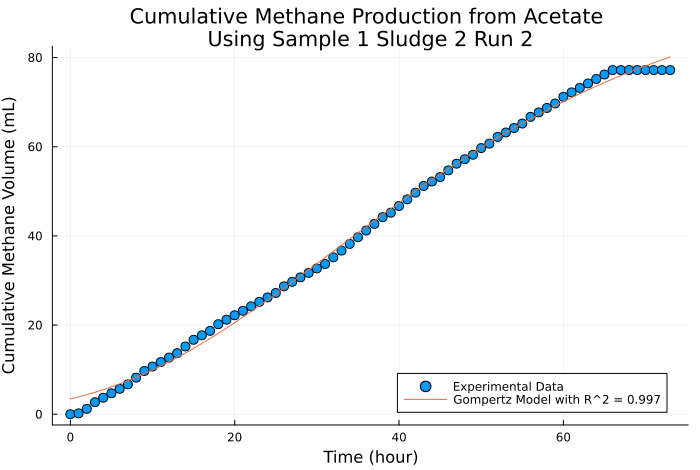
\includegraphics[width=.9\linewidth]{../plots/BMPs/Acetate/methane_kinetics_acet_test_1_s2_2_hour.png}
\end{center}

\begin{center}
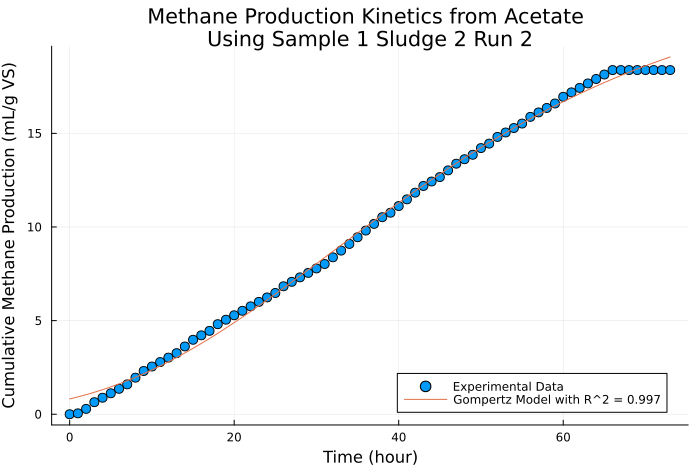
\includegraphics[width=.9\linewidth]{../plots/BMPs/Acetate/specific_methane_kinetics_acet_test_1_s2_2_hour.png}
\end{center}

\subsection{Acetate Test 2}
\label{sec:org38a7c1b}
Το section αυτό αναφέρεται στη δοκιμή με 100 μL οξικό στο δείγμα (2).

\textbf{acet\textsubscript{test}\textsubscript{2}\textsubscript{s2}}
\begin{minted}[breaklines=true,breakanywhere=true]{julia}

### Data Analysis on Reactor 2 ###

<<date_saving_acetate_s2>>

inds = 4:21
exp_meth_vol = [0, 3.5, 3, 1, 1, 1, 0.2, 0.4, 0.4, 2, 0, 0, 0, 0, 0, 0, 0, 0]
meth_vol_acet_2 = cumsum(exp_meth_vol)[end]
exp_name = "acet_test_2_s2"
source = "Acetate"
reactor = "Reactor 2"
sludge = "Sludge 2"
run_num = "Run 1"
input_cod = 4.2
p0 = [30.0, 6.0, 1.0]

<<bmp_data_processing>>
max_rate_acet_2 = max_manual_rate

<<bmp_curve_fitting_min>>
model_acet_2 = vcat(reactor, round.(model_params, digits = 3), round(r_squared, digits = 3))
<<bmp_data_plotting>>

p0 = [7.1, 1.43, 1.0]
<<sma_curve_fitting_min>>
sma_acet_2 = vcat(reactor, round.(model_params, digits = 3), round(r_squared, digits = 3))  
<<bmp_data_plotting>>

return("../data/exp_pro/"*exp_name*".csv")
\end{minted}

\begin{minted}[breaklines=true,breakanywhere=true]{elisp}
(org-table-import-after-n-lines 4 <<acet_test_2_s2()>> '(4))
\end{minted}

\begin{table}[htbp]
\caption{Κινητικά Δεδομένα}
\centering
\begin{tabular}{lrrrr}
Timestamp & Seconds & Minutes & Methane\textsubscript{Volume} & Cumulative\textsubscript{Methane}\textsubscript{Volume}\\[0pt]
10/04\textsubscript{14}:02 & 0.0 & 0.0 & 0.0 & 0.0\\[0pt]
10/04\textsubscript{14}:03 & 60.0 & 1.0 & 3.5 & 3.5\\[0pt]
10/04\textsubscript{14}:04 & 108.292 & 1.8049 & 3.0 & 6.5\\[0pt]
10/04\textsubscript{14}:05 & 165.673 & 2.7612 & 1.0 & 7.5\\[0pt]
10/04\textsubscript{14}:06 & 225.695 & 3.7616 & 1.0 & 8.5\\[0pt]
10/04\textsubscript{14}:07 & 285.685 & 4.7614 & 1.0 & 9.5\\[0pt]
10/04\textsubscript{14}:07 & 304.274 & 5.0712 & 0.2 & 9.7\\[0pt]
10/04\textsubscript{14}:08 & 364.265 & 6.0711 & 0.4 & 10.1\\[0pt]
10/04\textsubscript{14}:08 & 392.287 & 6.5381 & 0.4 & 10.5\\[0pt]
10/04\textsubscript{14}:09 & 452.282 & 7.538 & 2.0 & 12.5\\[0pt]
10/04\textsubscript{14}:10 & 512.28 & 8.538 & 0.0 & 12.5\\[0pt]
10/04\textsubscript{14}:11 & 572.302 & 9.5384 & 0.0 & 12.5\\[0pt]
10/04\textsubscript{14}:12 & 632.313 & 10.5386 & 0.0 & 12.5\\[0pt]
10/04\textsubscript{14}:13 & 692.325 & 11.5388 & 0.0 & 12.5\\[0pt]
10/04\textsubscript{14}:14 & 752.33 & 12.5388 & 0.0 & 12.5\\[0pt]
10/04\textsubscript{14}:15 & 812.328 & 13.5388 & 0.0 & 12.5\\[0pt]
10/04\textsubscript{14}:16 & 872.318 & 14.5386 & 0.0 & 12.5\\[0pt]
10/04\textsubscript{14}:17 & 932.329 & 15.5388 & 0.0 & 12.5\\[0pt]
\end{tabular}
\end{table}

\begin{center}
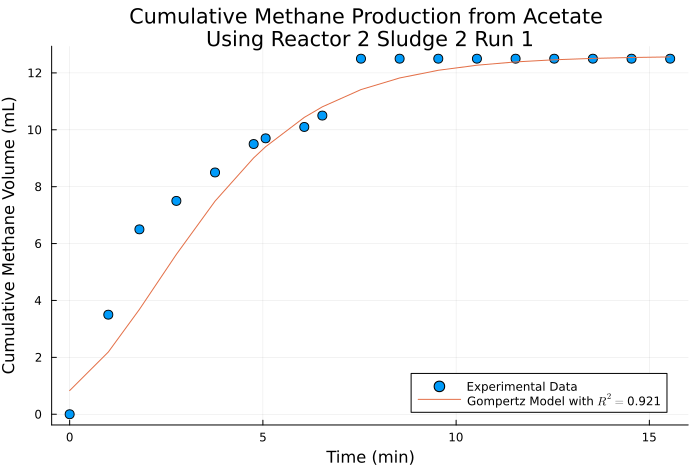
\includegraphics[width=.9\linewidth]{../plots/BMPs/Acetate/methane_kinetics_acet_test_2_s2_min.png}
\end{center}

\begin{center}
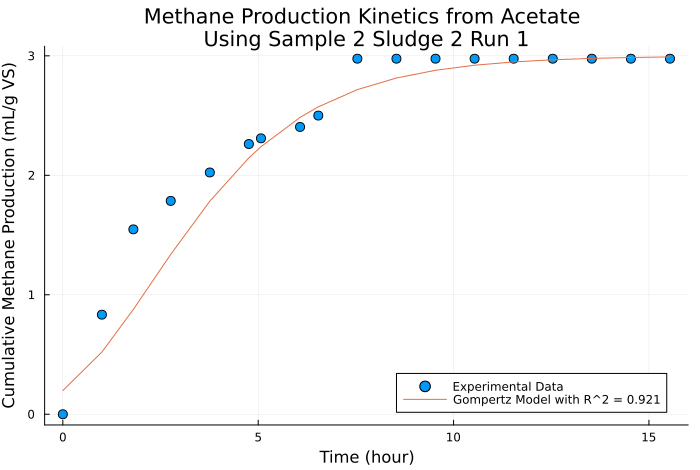
\includegraphics[width=.9\linewidth]{../plots/BMPs/Acetate/specific_methane_kinetics_acet_test_2_s2_min.png}
\end{center}

\subsubsection{Continued}
\label{sec:orgf032bd4}
Αυτό το section είναι για την συνέχεια του πειράματος, η οποία θα χρησιμοποιηθεί ως το negative blank για την ανάλυση των πειραμάτων με υδρόλυμα.

\begin{minted}[breaklines=true,breakanywhere=true]{julia}

<<date_saving_acetate_s2_2>>

inds = 1:90
exp_meth_vol = [0.5, 0.5, 0.3, 0.3, 0.5, 0.8, 0.8, 0.5, 0.5, 1, 0.5, 0.5, 0.5, 0.5, 0.5, 0.5, 0.5, 1, 1, 1, 1, 1.5, 1, 1.5, 1.5, 1, 1, 1, 1, 1, 1, 1, 1, 1, 1, 0.1, 0.1, 0.5, 0.5, 1, 1, 1, 1, 1, 1, 1, 1, 1, 1, 1, 1, 1, 1, 1, 1, 1, 1, 1, 1, 1, 1, 1, 1, 1, 1, 1, 1, 1, 1, 1, 1, 1, 1, 1, 1, 1, 1, 1, 1, 1, 1, 1, 1, 1, 0, 0, 0, 0, 0, 0]
meth_vol_acet_2 = cumsum(exp_meth_vol)[end]
exp_name = "acet_test_2_s2_2"
source = "Acetate"
reactor = "Reactor 2"
sludge = "Sludge 2"
run_num = "Run 2"
input_vs = 4.2
p0 = [90.0, 20.0, 1.0]

<<bmp_data_processing>>
max_rate_acet_2_2 = max_manual_rate

<<bmp_curve_fitting_hour>>
model_acet_2 = vcat(reactor, round.(model_params, digits = 3), round(r_squared, digits = 3))
<<bmp_data_plotting>>

<<sma_curve_fitting_hour>>
sma_acet_2 = vcat(reactor, round.(model_params, digits = 3), round(r_squared, digits = 3))  
<<bmp_data_plotting>>

return("../data/exp_pro/"*exp_name*".csv")

\end{minted}

\begin{minted}[breaklines=true,breakanywhere=true]{elisp}
(org-table-import-after-n-lines 3 <<acet_test_2_s2_2()>> '(4))
\end{minted}

\begin{center}
\begin{tabular}{lrrrr}
Timestamp & Seconds & Minutes & Methane\textsubscript{Volume} & Cumulative\textsubscript{Methane}\textsubscript{Volume}\\[0pt]
10/04\textsubscript{21}:34 & 0.0 & 0.0 & 0.5 & 0.5\\[0pt]
10/04\textsubscript{22}:34 & 3600.039 & 60.0006 & 0.5 & 1.0\\[0pt]
10/04\textsubscript{23}:34 & 7200.685 & 120.0114 & 0.3 & 1.3\\[0pt]
11/04\textsubscript{00}:34 & 10800.728 & 180.0121 & 0.3 & 1.6\\[0pt]
11/04\textsubscript{01}:34 & 14400.775 & 240.0129 & 0.5 & 2.1\\[0pt]
11/04\textsubscript{02}:34 & 18000.813 & 300.0136 & 0.8 & 2.9\\[0pt]
11/04\textsubscript{03}:34 & 21600.863 & 360.0144 & 0.8 & 3.7\\[0pt]
11/04\textsubscript{04}:34 & 25200.653 & 420.0109 & 0.5 & 4.2\\[0pt]
11/04\textsubscript{05}:34 & 28800.632 & 480.0105 & 0.5 & 4.7\\[0pt]
11/04\textsubscript{06}:34 & 32400.629 & 540.0105 & 1.5 & 6.2\\[0pt]
11/04\textsubscript{07}:34 & 36000.642 & 600.0107 & 1.0 & 7.2\\[0pt]
11/04\textsubscript{08}:34 & 39600.671 & 660.0112 & 1.0 & 8.2\\[0pt]
11/04\textsubscript{09}:34 & 43200.688 & 720.0115 & 1.0 & 9.2\\[0pt]
11/04\textsubscript{10}:34 & 46800.715 & 780.0119 & 1.0 & 10.2\\[0pt]
11/04\textsubscript{11}:34 & 50400.729 & 840.0122 & 1.0 & 11.2\\[0pt]
11/04\textsubscript{12}:34 & 54000.755 & 900.0126 & 1.0 & 12.2\\[0pt]
11/04\textsubscript{13}:34 & 57601.133 & 960.0189 & 1.0 & 13.2\\[0pt]
11/04\textsubscript{14}:34 & 61201.256 & 1020.0209 & 1.0 & 14.2\\[0pt]
11/04\textsubscript{15}:34 & 64801.31 & 1080.0218 & 1.0 & 15.2\\[0pt]
11/04\textsubscript{16}:34 & 68401.341 & 1140.0224 & 1.0 & 16.2\\[0pt]
11/04\textsubscript{17}:34 & 72002.439 & 1200.0406 & 1.0 & 17.2\\[0pt]
11/04\textsubscript{18}:34 & 75602.47 & 1260.0412 & 1.5 & 18.7\\[0pt]
11/04\textsubscript{19}:34 & 79202.51 & 1320.0418 & 1.0 & 19.7\\[0pt]
11/04\textsubscript{20}:34 & 82802.529 & 1380.0422 & 1.5 & 21.2\\[0pt]
11/04\textsubscript{21}:34 & 86402.574 & 1440.0429 & 1.5 & 22.7\\[0pt]
11/04\textsubscript{22}:34 & 90002.121 & 1500.0354 & 1.0 & 23.7\\[0pt]
11/04\textsubscript{23}:34 & 93601.969 & 1560.0328 & 1.0 & 24.7\\[0pt]
12/04\textsubscript{00}:34 & 97201.968 & 1620.0328 & 1.0 & 25.7\\[0pt]
12/04\textsubscript{01}:34 & 100801.993 & 1680.0332 & 1.0 & 26.7\\[0pt]
12/04\textsubscript{02}:34 & 104401.982 & 1740.033 & 1.0 & 27.7\\[0pt]
12/04\textsubscript{03}:34 & 108001.988 & 1800.0331 & 1.0 & 28.7\\[0pt]
12/04\textsubscript{04}:34 & 111601.986 & 1860.0331 & 1.0 & 29.7\\[0pt]
12/04\textsubscript{05}:34 & 115201.981 & 1920.033 & 1.0 & 30.7\\[0pt]
12/04\textsubscript{06}:34 & 118801.988 & 1980.0331 & 1.0 & 31.7\\[0pt]
12/04\textsubscript{07}:34 & 122402.22 & 2040.037 & 1.0 & 32.7\\[0pt]
12/04\textsubscript{08}:34 & 126002.462 & 2100.041 & 0.1 & 32.8\\[0pt]
12/04\textsubscript{09}:34 & 129602.529 & 2160.0422 & 0.1 & 32.9\\[0pt]
12/04\textsubscript{10}:34 & 133202.561 & 2220.0427 & 0.5 & 33.4\\[0pt]
12/04\textsubscript{11}:34 & 136802.563 & 2280.0427 & 0.5 & 33.9\\[0pt]
12/04\textsubscript{12}:34 & 140402.562 & 2340.0427 & 1.0 & 34.9\\[0pt]
12/04\textsubscript{13}:34 & 144002.56 & 2400.0427 & 1.0 & 35.9\\[0pt]
12/04\textsubscript{14}:34 & 147602.565 & 2460.0428 & 1.0 & 36.9\\[0pt]
12/04\textsubscript{15}:34 & 151202.563 & 2520.0427 & 1.0 & 37.9\\[0pt]
12/04\textsubscript{16}:34 & 154802.936 & 2580.0489 & 1.0 & 38.9\\[0pt]
12/04\textsubscript{17}:34 & 158403.259 & 2640.0543 & 1.0 & 39.9\\[0pt]
12/04\textsubscript{18}:34 & 162003.266 & 2700.0544 & 1.0 & 40.9\\[0pt]
12/04\textsubscript{19}:34 & 165603.263 & 2760.0544 & 1.0 & 41.9\\[0pt]
12/04\textsubscript{20}:34 & 169203.271 & 2820.0545 & 1.0 & 42.9\\[0pt]
12/04\textsubscript{21}:34 & 172803.268 & 2880.0545 & 1.0 & 43.9\\[0pt]
12/04\textsubscript{22}:34 & 176403.274 & 2940.0546 & 1.0 & 44.9\\[0pt]
12/04\textsubscript{23}:34 & 180003.713 & 3000.0619 & 1.0 & 45.9\\[0pt]
13/04\textsubscript{00}:34 & 183603.711 & 3060.0618 & 1.0 & 46.9\\[0pt]
13/04\textsubscript{01}:34 & 187203.714 & 3120.0619 & 1.0 & 47.9\\[0pt]
13/04\textsubscript{02}:34 & 190803.733 & 3180.0622 & 1.0 & 48.9\\[0pt]
13/04\textsubscript{03}:34 & 194403.734 & 3240.0622 & 1.0 & 49.9\\[0pt]
13/04\textsubscript{04}:34 & 198003.74 & 3300.0623 & 1.0 & 50.9\\[0pt]
13/04\textsubscript{05}:34 & 201603.729 & 3360.0622 & 1.0 & 51.9\\[0pt]
13/04\textsubscript{06}:34 & 205203.735 & 3420.0622 & 1.0 & 52.9\\[0pt]
13/04\textsubscript{07}:34 & 208803.732 & 3480.0622 & 1.0 & 53.9\\[0pt]
13/04\textsubscript{08}:34 & 212403.729 & 3540.0622 & 1.0 & 54.9\\[0pt]
13/04\textsubscript{09}:34 & 216003.736 & 3600.0623 & 1.0 & 55.9\\[0pt]
13/04\textsubscript{10}:34 & 219604.073 & 3660.0679 & 1.0 & 56.9\\[0pt]
13/04\textsubscript{11}:34 & 223204.478 & 3720.0746 & 1.0 & 57.9\\[0pt]
13/04\textsubscript{12}:34 & 226804.579 & 3780.0763 & 1.0 & 58.9\\[0pt]
13/04\textsubscript{13}:34 & 230404.66 & 3840.0777 & 1.0 & 59.9\\[0pt]
13/04\textsubscript{14}:34 & 234004.71 & 3900.0785 & 1.0 & 60.9\\[0pt]
13/04\textsubscript{15}:34 & 237604.74 & 3960.079 & 1.0 & 61.9\\[0pt]
13/04\textsubscript{16}:34 & 241204.792 & 4020.0799 & 1.0 & 62.9\\[0pt]
13/04\textsubscript{17}:34 & 244805.028 & 4080.0838 & 1.0 & 63.9\\[0pt]
13/04\textsubscript{18}:34 & 248405.035 & 4140.0839 & 1.0 & 64.9\\[0pt]
13/04\textsubscript{19}:34 & 252005.043 & 4200.0841 & 1.0 & 65.9\\[0pt]
13/04\textsubscript{20}:34 & 255605.136 & 4260.0856 & 1.0 & 66.9\\[0pt]
13/04\textsubscript{21}:34 & 259205.148 & 4320.0858 & 1.0 & 67.9\\[0pt]
13/04\textsubscript{22}:34 & 262805.165 & 4380.0861 & 1.0 & 68.9\\[0pt]
13/04\textsubscript{23}:34 & 266405.163 & 4440.086 & 1.0 & 69.9\\[0pt]
14/04\textsubscript{00}:34 & 270005.17 & 4500.0862 & 1.0 & 70.9\\[0pt]
14/04\textsubscript{01}:34 & 273605.167 & 4560.0861 & 1.0 & 71.9\\[0pt]
14/04\textsubscript{02}:34 & 277205.164 & 4620.0861 & 1.0 & 72.9\\[0pt]
14/04\textsubscript{03}:34 & 280805.172 & 4680.0862 & 1.0 & 73.9\\[0pt]
14/04\textsubscript{04}:34 & 284405.351 & 4740.0892 & 1.0 & 74.9\\[0pt]
14/04\textsubscript{05}:34 & 288005.714 & 4800.0952 & 1.0 & 75.9\\[0pt]
14/04\textsubscript{06}:34 & 291605.861 & 4860.0977 & 1.0 & 76.9\\[0pt]
14/04\textsubscript{07}:34 & 295205.912 & 4920.0985 & 1.0 & 77.9\\[0pt]
14/04\textsubscript{08}:34 & 298805.966 & 4980.0994 & 1.0 & 78.9\\[0pt]
14/04\textsubscript{09}:34 & 302406.001 & 5040.1 & 0.0 & 78.9\\[0pt]
14/04\textsubscript{10}:34 & 306006.043 & 5100.1007 & 0.0 & 78.9\\[0pt]
14/04\textsubscript{11}:34 & 309606.076 & 5160.1013 & 0.0 & 78.9\\[0pt]
14/04\textsubscript{12}:34 & 313206.518 & 5220.1086 & 0.0 & 78.9\\[0pt]
14/04\textsubscript{13}:34 & 316806.546 & 5280.1091 & 0.0 & 78.9\\[0pt]
14/04\textsubscript{14}:34 & 320406.524 & 5340.1087 & 0.0 & 78.9\\[0pt]
\end{tabular}
\end{center}

\begin{center}
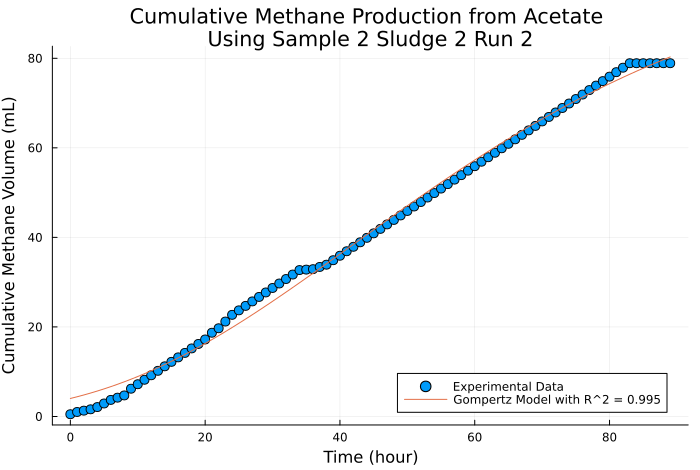
\includegraphics[width=.9\linewidth]{../plots/BMPs/Acetate/methane_kinetics_acet_test_2_s2_2_hour.png}
\end{center}

\begin{center}
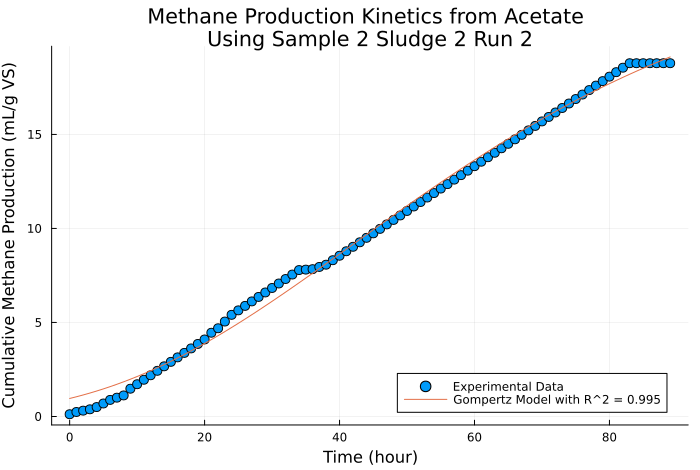
\includegraphics[width=.9\linewidth]{../plots/BMPs/Acetate/specific_methane_kinetics_acet_test_2_s2_2_hour.png}
\end{center}

\subsection{Acetate Test 4}
\label{sec:org02ed6ed}
Το section αυτό αναφέρεται στη δοκιμή με 100 μL οξικό στο δείγμα (4).

\textbf{acet\textsubscript{test}\textsubscript{4}\textsubscript{s2}}
\begin{minted}[breaklines=true,breakanywhere=true]{julia}

### Data Analysis on Reactor 4 ###

<<date_saving_acetate_s2>>

inds = 10:21
exp_meth_vol = [0, 5.5, 2.0, 1.5, 0.5, 0, 0, 0, 0, 0, 0, 0]
meth_vol_acet_4 = cumsum(exp_meth_vol)[end]
exp_name = "acet_test_4_s2"
source = "Acetate"
reactor = "Reactor 4"
sludge = "Sludge 2"
run_num = "Run 1"
input_vs = 4.2
p0 = [40.0, 10.0, 1.0]

<<bmp_data_processing>>
max_rate_acet_4 = max_manual_rate

<<bmp_curve_fitting_min>>
model_acet_4 = vcat(reactor, round.(model_params, digits = 3), round(r_squared, digits = 3))
<<bmp_data_plotting>>

<<sma_curve_fitting_min>>
sma_acet_4 = vcat(reactor, round.(model_params, digits = 3), round(r_squared, digits = 3))  
<<bmp_data_plotting>>

return("../data/exp_pro/"*exp_name*".csv")
\end{minted}

\begin{minted}[breaklines=true,breakanywhere=true]{elisp}
(org-table-import-after-n-lines 4 <<acet_test_4_s2()>> '(4))
\end{minted}

\begin{table}[htbp]
\caption{Κινητικά δεδομένα}
\centering
\begin{tabular}{lrrrr}
Timestamp & Seconds & Minutes & Methane\textsubscript{Volume} & Cumulative\textsubscript{Methane}\textsubscript{Volume}\\[0pt]
10/04\textsubscript{14}:07 & 0.0 & 0.0 & 0.0 & 0.0\\[0pt]
10/04\textsubscript{14}:08 & 59.991 & 0.9998 & 5.5 & 5.5\\[0pt]
10/04\textsubscript{14}:08 & 88.013 & 1.4669 & 2.0 & 7.5\\[0pt]
10/04\textsubscript{14}:09 & 148.008 & 2.4668 & 1.5 & 9.0\\[0pt]
10/04\textsubscript{14}:10 & 208.006 & 3.4668 & 0.5 & 9.5\\[0pt]
10/04\textsubscript{14}:11 & 268.028 & 4.4671 & 0.0 & 9.5\\[0pt]
10/04\textsubscript{14}:12 & 328.039 & 5.4673 & 0.0 & 9.5\\[0pt]
10/04\textsubscript{14}:13 & 388.051 & 6.4675 & 0.0 & 9.5\\[0pt]
10/04\textsubscript{14}:14 & 448.056 & 7.4676 & 0.0 & 9.5\\[0pt]
10/04\textsubscript{14}:15 & 508.054 & 8.4676 & 0.0 & 9.5\\[0pt]
10/04\textsubscript{14}:16 & 568.044 & 9.4674 & 0.0 & 9.5\\[0pt]
10/04\textsubscript{14}:17 & 628.055 & 10.4676 & 0.0 & 9.5\\[0pt]
\end{tabular}
\end{table}

\begin{center}
\includegraphics[width=.9\linewidth]{../plots/BMPs/Acetate/methane_kinetics_acet_test_4_s2_min.png}
\end{center}

\begin{center}
\includegraphics[width=.9\linewidth]{../plots/BMPs/Acetate/specific_methane_kinetics_acet_test_4_s2.png}
\end{center}

\subsubsection{Continued}
\label{sec:org1d616d5}
Αυτό το section είναι για την συνέχεια του πειράματος, η οποία θα χρησιμοποιηθεί ως το negative blank για την ανάλυση των πειραμάτων με υδρόλυμα.

\begin{minted}[breaklines=true,breakanywhere=true]{julia}

<<date_saving_acetate_s2_2>>

inds = 13:110
exp_meth_vol = [1, 0.5, 0.6, 0.5, 0.5, 0.5, 1, 0.5, 0.8, 0.2, 0.5, 0.5, 0.5, 1, 0.5, 1, 0.5, 1, 1, 0.5, 1, 1, 1, 1, 1, 0.1, 0.1, 0.1, 0.2, 0.2, 0.2, 0.1, 1.5, 1, 0.5, 0.5, 1, 1, 0.5, 0.5, 0.7, 0.7, 0.5, 1, 0.5, 0.5, 0.8, 0.6, 0.3, 0.5, 0.5, 1, 1, 1, 1, 0.8, 0.5, 1, 0.5, 0.5, 0.5, 1, 0.5, 0.5, 1, 1, 0.5, 0.5, 1, 0.5, 0.5, 1, 0.5, 0.5, 0.5, 0.5, 0.3, 0.3, 0.3, 0.5, 0.5, 0.5, 1, 0.5, 0.5, 0.5, 0.5, 0.5, 0.5, 0.5, 0.5, 0.5, 0.5, 0, 0, 0, 0, 0]
meth_vol_acet_4 = cumsum(exp_meth_vol)[end]
exp_name = "acet_test_4_s2_2"
source = "Acetate"
reactor = "Reactor 4"
sludge = "Sludge 2"
run_num = "Run 2"
input_vs = 4.2
p4 = [90.0, 20.0, 1.0]

<<bmp_data_processing>>
max_rate_acet_4_2 = max_manual_rate

<<bmp_curve_fitting_hour>>
model_acet_4 = vcat(reactor, round.(model_params, digits = 3), round(r_squared, digits = 3))
<<bmp_data_plotting>>

<<sma_curve_fitting_hour>>
sma_acet_4 = vcat(reactor, round.(model_params, digits = 3), round(r_squared, digits = 3))  
<<bmp_data_plotting>>

return("../data/exp_pro/"*exp_name*".csv")

\end{minted}

\begin{minted}[breaklines=true,breakanywhere=true]{elisp}
(org-table-import-after-n-lines 3 <<acet_test_4_s2_2()>> '(4))
\end{minted}

\begin{center}
\begin{tabular}{lrrrr}
Timestamp & Seconds & Minutes & Methane\textsubscript{Volume} & Cumulative\textsubscript{Methane}\textsubscript{Volume}\\[0pt]
11/04\textsubscript{09}:34 & 0.0 & 0.0 & 1.0 & 1.0\\[0pt]
11/04\textsubscript{10}:34 & 3600.027 & 60.0004 & 0.5 & 1.5\\[0pt]
11/04\textsubscript{11}:34 & 7200.041 & 120.0007 & 0.6 & 2.1\\[0pt]
11/04\textsubscript{12}:34 & 10800.067 & 180.0011 & 0.5 & 2.6\\[0pt]
11/04\textsubscript{13}:34 & 14400.445 & 240.0074 & 0.5 & 3.1\\[0pt]
11/04\textsubscript{14}:34 & 18000.568 & 300.0095 & 0.5 & 3.6\\[0pt]
11/04\textsubscript{15}:34 & 21600.622 & 360.0104 & 1.0 & 4.6\\[0pt]
11/04\textsubscript{16}:34 & 25200.653 & 420.0109 & 0.5 & 5.1\\[0pt]
11/04\textsubscript{17}:34 & 28801.751 & 480.0292 & 0.8 & 5.9\\[0pt]
11/04\textsubscript{18}:34 & 32401.782 & 540.0297 & 0.2 & 6.1\\[0pt]
11/04\textsubscript{19}:34 & 36001.822 & 600.0304 & 0.5 & 6.6\\[0pt]
11/04\textsubscript{20}:34 & 39601.841 & 660.0307 & 0.5 & 7.1\\[0pt]
11/04\textsubscript{21}:34 & 43201.886 & 720.0314 & 0.5 & 7.6\\[0pt]
11/04\textsubscript{22}:34 & 46801.433 & 780.0239 & 1.0 & 8.6\\[0pt]
11/04\textsubscript{23}:34 & 50401.281 & 840.0214 & 0.5 & 9.1\\[0pt]
12/04\textsubscript{00}:34 & 54001.28 & 900.0213 & 1.0 & 10.1\\[0pt]
12/04\textsubscript{01}:34 & 57601.305 & 960.0218 & 0.5 & 10.6\\[0pt]
12/04\textsubscript{02}:34 & 61201.294 & 1020.0216 & 1.0 & 11.6\\[0pt]
12/04\textsubscript{03}:34 & 64801.3 & 1080.0217 & 1.0 & 12.6\\[0pt]
12/04\textsubscript{04}:34 & 68401.298 & 1140.0216 & 0.5 & 13.1\\[0pt]
12/04\textsubscript{05}:34 & 72001.293 & 1200.0216 & 1.0 & 14.1\\[0pt]
12/04\textsubscript{06}:34 & 75601.3 & 1260.0217 & 1.0 & 15.1\\[0pt]
12/04\textsubscript{07}:34 & 79201.532 & 1320.0255 & 1.0 & 16.1\\[0pt]
12/04\textsubscript{08}:34 & 82801.774 & 1380.0296 & 1.0 & 17.1\\[0pt]
12/04\textsubscript{09}:34 & 86401.841 & 1440.0307 & 1.0 & 18.1\\[0pt]
12/04\textsubscript{10}:34 & 90001.873 & 1500.0312 & 0.1 & 18.2\\[0pt]
12/04\textsubscript{11}:34 & 93601.875 & 1560.0312 & 0.1 & 18.3\\[0pt]
12/04\textsubscript{12}:34 & 97201.874 & 1620.0312 & 0.1 & 18.4\\[0pt]
12/04\textsubscript{13}:34 & 100801.872 & 1680.0312 & 0.2 & 18.6\\[0pt]
12/04\textsubscript{14}:34 & 104401.877 & 1740.0313 & 0.2 & 18.8\\[0pt]
12/04\textsubscript{15}:34 & 108001.875 & 1800.0312 & 0.2 & 19.0\\[0pt]
12/04\textsubscript{16}:34 & 111602.248 & 1860.0375 & 0.1 & 19.1\\[0pt]
12/04\textsubscript{17}:34 & 115202.571 & 1920.0428 & 1.5 & 20.6\\[0pt]
12/04\textsubscript{18}:34 & 118802.578 & 1980.043 & 1.0 & 21.6\\[0pt]
12/04\textsubscript{19}:34 & 122402.575 & 2040.0429 & 0.5 & 22.1\\[0pt]
12/04\textsubscript{20}:34 & 126002.583 & 2100.0431 & 0.5 & 22.6\\[0pt]
12/04\textsubscript{21}:34 & 129602.58 & 2160.043 & 1.0 & 23.6\\[0pt]
12/04\textsubscript{22}:34 & 133202.586 & 2220.0431 & 1.0 & 24.6\\[0pt]
12/04\textsubscript{23}:34 & 136803.025 & 2280.0504 & 0.5 & 25.1\\[0pt]
13/04\textsubscript{00}:34 & 140403.023 & 2340.0504 & 0.5 & 25.6\\[0pt]
13/04\textsubscript{01}:34 & 144003.026 & 2400.0504 & 0.7 & 26.3\\[0pt]
13/04\textsubscript{02}:34 & 147603.045 & 2460.0508 & 0.7 & 27.0\\[0pt]
13/04\textsubscript{03}:34 & 151203.046 & 2520.0508 & 0.5 & 27.5\\[0pt]
13/04\textsubscript{04}:34 & 154803.052 & 2580.0509 & 1.0 & 28.5\\[0pt]
13/04\textsubscript{05}:34 & 158403.041 & 2640.0507 & 0.5 & 29.0\\[0pt]
13/04\textsubscript{06}:34 & 162003.047 & 2700.0508 & 0.5 & 29.5\\[0pt]
13/04\textsubscript{07}:34 & 165603.044 & 2760.0507 & 0.8 & 30.3\\[0pt]
13/04\textsubscript{08}:34 & 169203.041 & 2820.0507 & 0.6 & 30.9\\[0pt]
13/04\textsubscript{09}:34 & 172803.048 & 2880.0508 & 0.3 & 31.2\\[0pt]
13/04\textsubscript{10}:34 & 176403.385 & 2940.0564 & 0.5 & 31.7\\[0pt]
13/04\textsubscript{11}:34 & 180003.79 & 3000.0632 & 0.5 & 32.2\\[0pt]
13/04\textsubscript{12}:34 & 183603.891 & 3060.0649 & 1.0 & 33.2\\[0pt]
13/04\textsubscript{13}:34 & 187203.972 & 3120.0662 & 1.0 & 34.2\\[0pt]
13/04\textsubscript{14}:34 & 190804.022 & 3180.067 & 1.0 & 35.2\\[0pt]
13/04\textsubscript{15}:34 & 194404.052 & 3240.0675 & 1.0 & 36.2\\[0pt]
13/04\textsubscript{16}:34 & 198004.104 & 3300.0684 & 0.8 & 37.0\\[0pt]
13/04\textsubscript{17}:34 & 201604.34 & 3360.0723 & 0.5 & 37.5\\[0pt]
13/04\textsubscript{18}:34 & 205204.347 & 3420.0724 & 1.0 & 38.5\\[0pt]
13/04\textsubscript{19}:34 & 208804.355 & 3480.0726 & 0.5 & 39.0\\[0pt]
13/04\textsubscript{20}:34 & 212404.448 & 3540.0741 & 0.5 & 39.5\\[0pt]
13/04\textsubscript{21}:34 & 216004.46 & 3600.0743 & 0.5 & 40.0\\[0pt]
13/04\textsubscript{22}:34 & 219604.477 & 3660.0746 & 1.0 & 41.0\\[0pt]
13/04\textsubscript{23}:34 & 223204.475 & 3720.0746 & 0.5 & 41.5\\[0pt]
14/04\textsubscript{00}:34 & 226804.482 & 3780.0747 & 0.5 & 42.0\\[0pt]
14/04\textsubscript{01}:34 & 230404.479 & 3840.0746 & 1.0 & 43.0\\[0pt]
14/04\textsubscript{02}:34 & 234004.476 & 3900.0746 & 1.0 & 44.0\\[0pt]
14/04\textsubscript{03}:34 & 237604.484 & 3960.0747 & 0.5 & 44.5\\[0pt]
14/04\textsubscript{04}:34 & 241204.663 & 4020.0777 & 0.5 & 45.0\\[0pt]
14/04\textsubscript{05}:34 & 244805.026 & 4080.0838 & 1.0 & 46.0\\[0pt]
14/04\textsubscript{06}:34 & 248405.173 & 4140.0862 & 0.5 & 46.5\\[0pt]
14/04\textsubscript{07}:34 & 252005.224 & 4200.0871 & 0.5 & 47.0\\[0pt]
14/04\textsubscript{08}:34 & 255605.278 & 4260.088 & 1.0 & 48.0\\[0pt]
14/04\textsubscript{09}:34 & 259205.313 & 4320.0886 & 0.5 & 48.5\\[0pt]
14/04\textsubscript{10}:34 & 262805.355 & 4380.0892 & 0.5 & 49.0\\[0pt]
14/04\textsubscript{11}:34 & 266405.388 & 4440.0898 & 0.5 & 49.5\\[0pt]
14/04\textsubscript{12}:34 & 270005.83 & 4500.0972 & 0.5 & 50.0\\[0pt]
14/04\textsubscript{13}:34 & 273605.858 & 4560.0976 & 0.3 & 50.3\\[0pt]
14/04\textsubscript{14}:34 & 277205.836 & 4620.0973 & 0.3 & 50.6\\[0pt]
14/04\textsubscript{15}:34 & 280805.835 & 4680.0972 & 0.3 & 50.9\\[0pt]
14/04\textsubscript{16}:34 & 284405.864 & 4740.0977 & 0.5 & 51.4\\[0pt]
14/04\textsubscript{17}:34 & 288006.052 & 4800.1009 & 0.5 & 51.9\\[0pt]
14/04\textsubscript{18}:34 & 291606.049 & 4860.1008 & 0.5 & 52.4\\[0pt]
14/04\textsubscript{19}:34 & 295206.13 & 4920.1022 & 1.0 & 53.4\\[0pt]
14/04\textsubscript{20}:34 & 298806.063 & 4980.101 & 0.5 & 53.9\\[0pt]
14/04\textsubscript{21}:34 & 302406.058 & 5040.101 & 0.5 & 54.4\\[0pt]
14/04\textsubscript{22}:34 & 306006.057 & 5100.101 & 0.5 & 54.9\\[0pt]
14/04\textsubscript{23}:34 & 309606.656 & 5160.1109 & 0.5 & 55.4\\[0pt]
15/04\textsubscript{00}:34 & 313206.758 & 5220.1126 & 0.5 & 55.9\\[0pt]
15/04\textsubscript{01}:34 & 316806.799 & 5280.1133 & 0.5 & 56.4\\[0pt]
15/04\textsubscript{02}:34 & 320406.8 & 5340.1133 & 0.5 & 56.9\\[0pt]
15/04\textsubscript{03}:34 & 324006.809 & 5400.1135 & 0.5 & 57.4\\[0pt]
15/04\textsubscript{04}:34 & 327606.805 & 5460.1134 & 0.5 & 57.9\\[0pt]
15/04\textsubscript{05}:34 & 331206.816 & 5520.1136 & 0.5 & 58.4\\[0pt]
15/04\textsubscript{06}:34 & 334806.812 & 5580.1135 & 0.0 & 58.4\\[0pt]
15/04\textsubscript{07}:34 & 338406.807 & 5640.1134 & 0.0 & 58.4\\[0pt]
15/04\textsubscript{08}:34 & 342007.021 & 5700.117 & 0.0 & 58.4\\[0pt]
15/04\textsubscript{09}:34 & 345607.096 & 5760.1183 & 0.0 & 58.4\\[0pt]
15/04\textsubscript{10}:34 & 349207.138 & 5820.119 & 0.0 & 58.4\\[0pt]
\end{tabular}
\end{center}

\begin{center}
\includegraphics[width=.9\linewidth]{../plots/BMPs/Acetate/methane_kinetics_acet_test_4_s2_2_hour.png}
\end{center}

\begin{center}
\includegraphics[width=.9\linewidth]{../plots/BMPs/Acetate/specific_methane_kinetics_acet_test_4_s2_2_hour.png}
\end{center}

\subsection{Update all helper}
\label{sec:orgec29b64}
Σε αυτό το section θα υπάρχει ένα helper code block που θα κάνει evaluate όλα τα παραπάνω. Έτσι, αν αλλάξει κάτι το οποίο επηρεάζει περισσότερα από ένα code blocks, θα μπορούν να γίνουν updated ταυτόχρονα πιο εύκολα. Επίσης, μία επιπλέον χρησιμότητα του code block αυτού είναι ότι αποθηκεύει ένα CSV που συγκεντρώνει όλα τα δεδομένα των κινητικών παραμέτρων από την προσαρμογή που έγινε παραπάνω, το οποίο είναι χρήσιμο για συγκρίσεις, παρόλο που τα συγκεκριμένα πειράματα δεν είναι τόσο σημαντικό να συγκριθούν.
\textbf{update\textsubscript{acetate}\textsubscript{tests}\textsubscript{s2}}
\begin{minted}[breaklines=true,breakanywhere=true]{julia}

<<acet_test_0_s2>>
<<acet_test_1_s2>>
<<acet_test_2_s2>>
<<acet_test_4_s2>>
<<acet_test_fw_s2>>

model_fit_table = Tables.table(vcat(reshape(model_acet_0, 1, 5), reshape(model_acet_1, 1, 5), reshape(model_acet_2, 1, 5), reshape(model_acet_4, 1, 5), reshape(model_acet_fw, 1, 5)), header = [:Reactor_Name, :Production_Potential, :Production_Rate, :Lag_Time, :R_squared])
CSV.write(datadir("exp_pro", "methane_from_acetate_kinetics_s2.csv"), model_fit_table)
return("../data/exp_pro/methane_from_acetate_kinetics_s2.csv")
\end{minted}

\begin{minted}[breaklines=true,breakanywhere=true]{elisp}
(org-table-import-after-n-lines 4 <<update_acetate_tests_s2()>> '(4))
\end{minted}

\begin{table}[htbp]
\caption{Kinetic Models in Minutes}
\centering
\begin{tabular}{lrrrr}
Reactor\textsubscript{Name} & Production\textsubscript{Potential} & Production\textsubscript{Rate} & Lag\textsubscript{Time} & R\textsubscript{squared}\\[0pt]
Reactor 0 & 6.955 & 7.392 & 0.165 & 0.996\\[0pt]
Reactor 1 & 11.663 & 3.444 & 0.0 & 0.843\\[0pt]
Reactor 2 & 12.599 & 2.038 & 0.0 & 0.921\\[0pt]
Reactor 4 & 9.484 & 6.821 & 0.194 & 0.999\\[0pt]
Reactor FW & 14.451 & 4.298 & 0.586 & 0.993\\[0pt]
\end{tabular}
\end{table}

\begin{minted}[breaklines=true,breakanywhere=true]{julia}

<<acet_test_0_s2>>
<<acet_test_1_s2>>
<<acet_test_2_s2>>
<<acet_test_4_s2>>
<<acet_test_fw_s2>>

sma_table = Tables.table(vcat(reshape(sma_acet_0, 1, 5), reshape(sma_acet_1, 1, 5), reshape(sma_acet_2, 1, 5), reshape(sma_acet_4, 1, 5), reshape(sma_acet_fw, 1, 5)), header = [:Reactor_Name, :Methane_Potential, :SMA, :Lag_Time, :R_sq])
CSV.write(datadir("exp_pro", "sma_from_acetate_s2.csv"), sma_table)

return("../data/exp_pro/sma_from_acetate_s2.csv")
\end{minted}

\begin{minted}[breaklines=true,breakanywhere=true]{elisp}
(org-table-import-after-n-lines 4 <<sma_acet_s2()>> '(4))
\end{minted}

\begin{table}[htbp]
\caption{SMA Kinetics in Minutes}
\centering
\begin{tabular}{lrrrr}
Reactor\textsubscript{Name} & Methane\textsubscript{Potential} & SMA & Lag\textsubscript{Time} & R\textsubscript{sq}\\[0pt]
Reactor 0 & 1.656 & 1.76 & 0.165 & 0.996\\[0pt]
Reactor 1 & 2.777 & 0.82 & 0.0 & 0.843\\[0pt]
Reactor 2 & 3.0 & 0.485 & 0.0 & 0.921\\[0pt]
Reactor 4 & 2.258 & 1.624 & 0.194 & 0.999\\[0pt]
Reactor FW & 3.441 & 1.023 & 0.586 & 0.993\\[0pt]
\end{tabular}
\end{table}

\subsubsection{Slow Growth Phase}
\label{sec:org088d528}
\textbf{update\textsubscript{acetate}\textsubscript{tests}\textsubscript{s2}\textsubscript{2}}
\begin{minted}[breaklines=true,breakanywhere=true]{julia}

<<acet_test_0_s2_2>>
<<acet_test_1_s2_2>>
<<acet_test_2_s2_2>>
<<acet_test_4_s2_2>>
<<acet_test_fw_s2_2>>

model_fit_table = Tables.table(vcat(reshape(model_acet_0, 1, 5), reshape(model_acet_1, 1, 5), reshape(model_acet_2, 1, 5), reshape(model_acet_4, 1, 5), reshape(model_acet_fw, 1, 5)), header = [:Reactor_Name, :Production_Potential, :Production_Rate, :Lag_Time, :R_squared])
CSV.write(datadir("exp_pro", "methane_from_acetate_kinetics_s2_2.csv"), model_fit_table)
return("../data/exp_pro/methane_from_acetate_kinetics_s2_2.csv")
\end{minted}

\begin{minted}[breaklines=true,breakanywhere=true]{elisp}
(org-table-import-after-n-lines 4 <<update_acetate_tests_s2_2()>> '(4))
\end{minted}

\begin{table}[htbp]
\caption{Kinetic Models in Hours}
\centering
\begin{tabular}{lrrrr}
Reactor\textsubscript{Name} & Production\textsubscript{Potential} & Production\textsubscript{Rate} & Lag\textsubscript{Time} & R\textsubscript{squared}\\[0pt]
Reactor 0 & 84.228 & 0.764 & 2.585 & 0.994\\[0pt]
Reactor 1 & 98.775 & 1.383 & 5.575 & 0.997\\[0pt]
Reactor 2 & 105.138 & 1.084 & 6.529 & 0.995\\[0pt]
Reactor 4 & 74.653 & 0.734 & 4.05 & 0.997\\[0pt]
Reactor FW & 60.343 & 0.766 & 1.903 & 0.998\\[0pt]
\end{tabular}
\end{table}

\begin{minted}[breaklines=true,breakanywhere=true]{julia}

<<acet_test_0_s2_2>>
<<acet_test_1_s2_2>>
<<acet_test_2_s2_2>>
<<acet_test_4_s2_2>>
<<acet_test_fw_s2_2>>

sma_table = Tables.table(vcat(reshape(sma_acet_0, 1, 5), reshape(sma_acet_1, 1, 5), reshape(sma_acet_2, 1, 5), reshape(sma_acet_4, 1, 5), reshape(sma_acet_fw, 1, 5)), header = [:Reactor_Name, :Methane_Potential, :SMA, :Lag_Time, :R_sq])
CSV.write(datadir("exp_pro", "sma_from_acet_s2_2.csv"), sma_table)

return("../data/exp_pro/sma_from_acet_s2_2.csv")
\end{minted}

\begin{minted}[breaklines=true,breakanywhere=true]{elisp}
(org-table-import-after-n-lines 4 <<sma_acet_s2_2()>> '(4))
\end{minted}

\begin{table}[htbp]
\caption{SMA Kinetics in Hours}
\centering
\begin{tabular}{lrrrr}
Reactor\textsubscript{Name} & Methane\textsubscript{Potential} & SMA & Lag\textsubscript{Time} & R\textsubscript{sq}\\[0pt]
Reactor 0 & 20.054 & 0.182 & 2.585 & 0.994\\[0pt]
Reactor 1 & 23.518 & 0.329 & 5.575 & 0.997\\[0pt]
Reactor 2 & 25.033 & 0.258 & 6.529 & 0.995\\[0pt]
Reactor 4 & 17.775 & 0.175 & 4.05 & 0.997\\[0pt]
Reactor FW & 14.367 & 0.182 & 1.903 & 0.998\\[0pt]
\end{tabular}
\end{table}

\subsection{Γενικά σχόλια για αυτόν τον κύκλο πειραμάτων}
\label{sec:orge197440}
Αυτά τα πειράματα έχουν ως σκοπό την σύγκριση με την προηγούμενη λάσπη και μία προσπάθεια επαλήθευσης των αποτελεσμάτων του προηγούμενου κύκλου χρησιμοποιώντας διαφορετική λάσπη (το οποίο θα μας επιτρέψει να επιβεβαιώσουμε πως λειτουργούν και οι 2 όπως θα αναμέναμε).

Με βάση τα αποτελέσματα του κύκλου αυτού, παρατηρούμε πως η λάσπη αυτή παράγει πολύ λιγότερο μεθάνιο. Βέβαια, μπορεί να παίζει ρόλο πως έχει προστεθεί αρκετά περισσότερη λάσπη στον αντιδραστήρα (250 g που αντιστοιχούν σε 4 g VS αντί για 125 g που αντιστοιχούσαν σε 1.5 g VS στο προηγούμενο πείραμα) οπότε ο λόγος τροφής προς μικροοργανισμούς (F/M) είναι πολύ μικρότερος.

Επίσης, παρατηρείται πως ο ρυθμός παραγωγής μεθανίου είναι μικρότερος (παρότι της ίδιας τάξης μεγέθους) από το προηγούμενο πείραμα, με εξαίρεση μόνο το δείγμα 0, όπου η λάσπη παρήγαγε πάρα πολύ γρήγορα αέριο.

Ως συμπέρασμα, βλέπουμε πως μία πιθανή αιτία για την μεγάλη διαφορά των δύο λασπών μπορεί να είναι η διαφορετική ποσότητα λάσπης (και άρα να πρέπει αυτή να ληφθεί υπόψην στις κινητικές) πέρα από το γεγονός ότι μπορεί να έχουν απλώς πολύ διαφορετική δραστικότητα.

\section{FW Hydrolysate Data Processing S2\textsubscript{R1}}
\label{sec:org80f385a}
Όπως αναφέρθηκε παραπάνω, τα δείγματα αυτά είχαν πάρα πολύ μεγάλη παραγωγή βιοαερίου, η οποία παρατηρήθηκε και στα πειράματα που τροφοδοτήσαμε με οξικό. Για τον λόγο αυτό, η παραγωγή εκείνη του οξικού θεωρήθηκε negative blank του πειράματος και θα αφαιρεθεί από όλα τα πειράματα.

\subsection{Reactor 0}
\label{sec:org815eaba}
Το δείγμα αυτό είναι labelled ως δείγμα 0 καθώς είναι το δείγμα το οποίο τροφοδοτήθηκε με treated FW, όμως χωρίς προσθήκη του μιξ ενζύμων και μικροοργανισμών. Όπως έχουμε δεί, όλες οι αντιδράσεις που γίνονται κατά την υδρόλυση και ζύμωση μπορούν να γίνουν και χωρίς το μιξ. Όμως, γινόντουσαν πιο αποτελεσματικά με την προσθήκη αυτού. Οπότε, ελπίζουμε πως το δείγμα αυτό θα έχει χειρότερα αποτελέσματα από τα άλλα, το οποίο θα μας οδηγήσει στην υπόθεση ότι το μιξ βελτιώνει όχι μόνο τα κριτήρια υδρόλυσης και οξεογένεσης αλλά και αυτό της μεθανογένεσης.

\textbf{hydrolysate\textsubscript{0}\textsubscript{s2}\textsubscript{r1}}
\begin{minted}[breaklines=true,breakanywhere=true]{julia}

### Data Analysis on Hydrolysate with 0 ml ###

<<acet_test_0_s2_2>>
meth_vol_blank = exp_meth_vol

<<date_saving_fw_s2_r1>>

inds = vcat(14:66, 93:160)
exp_meth_vol = [0, 0, 0.5, 0.6, 0.6, 0.7, 0.8, 0.7, 0.6, 0.7, 1, 0.9, 0.7, 0.8, 0.8, 0.7, 1, 1, 1, 0.8, 0.7, 1, 0.7, 0.7, 0.6, 1, 0.8, 1.5, 0.7, 1, 0.9, 0.8, 0.8, 1, 1, 1, 1, 1, 1, 1, 0.9, 1.2, 1, 0.9, 1, 0.8, 0.7, 0.8, 0.5, 0.5, 0.8, 0.5, 0.3, 0.5, 1.3, 1.2, 1, 1, 1, 0.5, 1, 1.2, 1, 1, 1, 1, 0.5, 1, 0.5, 0.5, 1, 1, 1, 1, 1, 1, 1, 1, 1, 0.9, 0.8, 0.7, 0.8, 0.6, 0.7, 0.9, 0.7, 0.7, 0.6, 0.5, 0.5, 0.5, 0.3, 0.2, 0.3, 0.4, 0.3, 0.2, 0.4, 0.4, 0.5, 0.3, 0.3, 0.3, 0.3, 0.4, 0.3, 0.3, 0.3, 0.2, 0.2, 0.2, 0.1, 0.1, 0.1, 0.1, 0, 0, 0, 0, 0]

meth_vol_blank_complete = vcat(meth_vol_blank, zeros(length(exp_meth_vol) - length(meth_vol_blank)))
meth_vol_diff = round.(exp_meth_vol .- meth_vol_blank_complete, digits = 1)
exp_meth_vol = [meth_vol_diff[i] < 0 ? meth_vol_diff[i] = 0.0 : meth_vol_diff[i] for i in 1:length(meth_vol_diff)]

meth_vol_hydro_0 = cumsum(exp_meth_vol)[end]

exp_name = "hydrolysate_0_s2_r1"
source = "Hydrolyzed FW"
reactor = "Reactor 0"
sludge = "Sludge 2"
run_num = "Run 1"
input_vs = 4.2

<<bmp_data_processing>>
max_rate_hydro_0 = max_manual_rate

# The same model is fit either with min or hour
p0 = [6.0, 0.01, 1.0]
<<bmp_curve_fitting_min>>
model_hydro_0_min = vcat(reactor, round.(model_params, digits = 3), round(r_squared, digits = 3))
<<bmp_data_plotting>>

p0 = [6.0, 0.2, 1.0]
<<bmp_curve_fitting_hour>>
model_hydro_0_hour = vcat(reactor, round.(model_params, digits = 3), round(r_squared, digits = 3))
<<bmp_data_plotting>>

p0 = [6.0, 10.0, 1.0]
<<sma_curve_fitting_hour>>
sma_hydro_0 = vcat(reactor, round.(model_params, digits = 3), round(r_squared, digits = 3))
<<bmp_data_plotting>>

return("../data/exp_pro/"*exp_name*".csv")
\end{minted}

\subsubsection{Results}
\label{sec:orgce96764}
Παρακάτω φαίνονται τα αποτελέσματα του σχετικού πειράματος.

\begin{minted}[breaklines=true,breakanywhere=true]{elisp}
(org-table-import-after-n-lines 3 <<hydrolysate_0_s2_r1()>> '(4))
\end{minted}

\begin{center}
\begin{tabular}{lrrrr}
Timestamp & Minutes & Hours & Methane\textsubscript{Volume} & Cumulative\textsubscript{Methane}\textsubscript{Volume}\\[0pt]
15/04\textsubscript{12}:21 & 0.0 & 0.0 & 0.0 & 0.0\\[0pt]
15/04\textsubscript{12}:29 & 7.3353 & 0.1223 & 0.0 & 0.0\\[0pt]
15/04\textsubscript{13}:29 & 67.3353 & 1.1223 & 0.0 & 0.0\\[0pt]
15/04\textsubscript{14}:29 & 127.3354 & 2.1223 & 0.1 & 0.1\\[0pt]
15/04\textsubscript{15}:29 & 187.3356 & 3.1223 & 0.0 & 0.1\\[0pt]
15/04\textsubscript{16}:29 & 247.3355 & 4.1223 & 0.0 & 0.1\\[0pt]
15/04\textsubscript{17}:29 & 307.3534 & 5.1226 & 0.0 & 0.1\\[0pt]
15/04\textsubscript{18}:29 & 367.3563 & 6.1226 & 0.2 & 0.3\\[0pt]
15/04\textsubscript{19}:29 & 427.3603 & 7.1227 & 0.1 & 0.4\\[0pt]
15/04\textsubscript{20}:29 & 487.3578 & 8.1226 & 0.2 & 0.6\\[0pt]
15/04\textsubscript{21}:29 & 547.3579 & 9.1226 & 0.0 & 0.6\\[0pt]
15/04\textsubscript{22}:29 & 607.3578 & 10.1226 & 0.0 & 0.6\\[0pt]
15/04\textsubscript{23}:29 & 667.3498 & 11.1225 & 0.0 & 0.6\\[0pt]
16/04\textsubscript{00}:29 & 727.3497 & 12.1225 & 0.3 & 0.9\\[0pt]
16/04\textsubscript{01}:29 & 787.3499 & 13.1225 & 0.3 & 1.2\\[0pt]
16/04\textsubscript{02}:29 & 847.3513 & 14.1225 & 0.2 & 1.4\\[0pt]
16/04\textsubscript{03}:29 & 907.353 & 15.1225 & 0.5 & 1.9\\[0pt]
16/04\textsubscript{04}:29 & 967.3532 & 16.1226 & 0.5 & 2.4\\[0pt]
16/04\textsubscript{05}:29 & 1027.3534 & 17.1226 & 0.5 & 2.9\\[0pt]
16/04\textsubscript{06}:29 & 1087.3534 & 18.1226 & 0.0 & 2.9\\[0pt]
16/04\textsubscript{07}:29 & 1147.3534 & 19.1226 & 0.0 & 2.9\\[0pt]
16/04\textsubscript{08}:29 & 1207.3536 & 20.1226 & 0.0 & 2.9\\[0pt]
16/04\textsubscript{09}:29 & 1267.3535 & 21.1226 & 0.0 & 2.9\\[0pt]
16/04\textsubscript{10}:26 & 1324.7359 & 22.0789 & 0.0 & 2.9\\[0pt]
16/04\textsubscript{11}:26 & 1384.7411 & 23.079 & 0.0 & 2.9\\[0pt]
16/04\textsubscript{12}:26 & 1444.7472 & 24.0791 & 0.0 & 2.9\\[0pt]
16/04\textsubscript{13}:26 & 1504.7468 & 25.0791 & 0.0 & 2.9\\[0pt]
16/04\textsubscript{14}:26 & 1564.747 & 26.0791 & 0.5 & 3.4\\[0pt]
16/04\textsubscript{15}:26 & 1624.7469 & 27.0791 & 0.2 & 3.6\\[0pt]
16/04\textsubscript{16}:26 & 1684.747 & 28.0791 & 0.5 & 4.1\\[0pt]
16/04\textsubscript{17}:26 & 1744.747 & 29.0791 & 0.4 & 4.5\\[0pt]
16/04\textsubscript{18}:26 & 1804.753 & 30.0792 & 0.6 & 5.1\\[0pt]
16/04\textsubscript{19}:26 & 1864.7527 & 31.0792 & 0.6 & 5.7\\[0pt]
16/04\textsubscript{20}:26 & 1924.7532 & 32.0792 & 0.5 & 6.2\\[0pt]
16/04\textsubscript{21}:26 & 1984.7553 & 33.0793 & 0.5 & 6.7\\[0pt]
16/04\textsubscript{22}:26 & 2044.756 & 34.0793 & 0.0 & 6.7\\[0pt]
16/04\textsubscript{23}:26 & 2104.7685 & 35.0795 & 0.0 & 6.7\\[0pt]
17/04\textsubscript{00}:26 & 2164.7684 & 36.0795 & 0.0 & 6.7\\[0pt]
17/04\textsubscript{01}:26 & 2224.7686 & 37.0795 & 0.5 & 7.2\\[0pt]
17/04\textsubscript{02}:26 & 2284.7685 & 38.0795 & 0.5 & 7.7\\[0pt]
17/04\textsubscript{03}:26 & 2344.7685 & 39.0795 & 0.4 & 8.1\\[0pt]
17/04\textsubscript{04}:26 & 2404.7685 & 40.0795 & 0.7 & 8.8\\[0pt]
17/04\textsubscript{05}:26 & 2464.7676 & 41.0795 & 0.5 & 9.3\\[0pt]
17/04\textsubscript{06}:26 & 2524.7664 & 42.0794 & 0.0 & 9.3\\[0pt]
17/04\textsubscript{07}:26 & 2584.7658 & 43.0794 & 0.5 & 9.8\\[0pt]
17/04\textsubscript{08}:26 & 2644.7659 & 44.0794 & 0.3 & 10.1\\[0pt]
17/04\textsubscript{09}:26 & 2704.7657 & 45.0794 & 0.2 & 10.3\\[0pt]
17/04\textsubscript{10}:29 & 2767.6056 & 46.1268 & 0.3 & 10.6\\[0pt]
17/04\textsubscript{11}:29 & 2827.6056 & 47.1268 & 0.0 & 10.6\\[0pt]
17/04\textsubscript{12}:29 & 2887.6267 & 48.1271 & 0.0 & 10.6\\[0pt]
17/04\textsubscript{13}:29 & 2947.6263 & 49.1271 & 0.3 & 10.9\\[0pt]
17/04\textsubscript{13}:57 & 2975.3544 & 49.5892 & 0.0 & 10.9\\[0pt]
17/04\textsubscript{14}:42 & 3020.0336 & 50.3339 & 0.0 & 10.9\\[0pt]
17/04\textsubscript{15}:17 & 3055.8519 & 50.9309 & 0.0 & 10.9\\[0pt]
17/04\textsubscript{16}:18 & 3116.8644 & 51.9477 & 0.8 & 11.7\\[0pt]
17/04\textsubscript{17}:18 & 3176.8632 & 52.9477 & 0.2 & 11.9\\[0pt]
17/04\textsubscript{18}:18 & 3236.8686 & 53.9478 & 0.0 & 11.9\\[0pt]
17/04\textsubscript{19}:18 & 3296.8686 & 54.9478 & 0.0 & 11.9\\[0pt]
17/04\textsubscript{20}:18 & 3356.8685 & 55.9478 & 0.0 & 11.9\\[0pt]
17/04\textsubscript{21}:18 & 3416.8685 & 56.9478 & 0.0 & 11.9\\[0pt]
17/04\textsubscript{22}:18 & 3476.8684 & 57.9478 & 0.5 & 12.4\\[0pt]
17/04\textsubscript{23}:18 & 3536.8684 & 58.9478 & 0.2 & 12.6\\[0pt]
18/04\textsubscript{00}:18 & 3596.8723 & 59.9479 & 0.0 & 12.6\\[0pt]
18/04\textsubscript{01}:18 & 3656.8742 & 60.9479 & 0.5 & 13.1\\[0pt]
18/04\textsubscript{02}:18 & 3716.8746 & 61.9479 & 0.5 & 13.6\\[0pt]
18/04\textsubscript{03}:18 & 3776.8751 & 62.9479 & 0.5 & 14.1\\[0pt]
18/04\textsubscript{04}:18 & 3836.8751 & 63.9479 & 0.0 & 14.1\\[0pt]
18/04\textsubscript{05}:18 & 3896.875 & 64.9479 & 0.0 & 14.1\\[0pt]
18/04\textsubscript{06}:18 & 3956.8751 & 65.9479 & 0.0 & 14.1\\[0pt]
18/04\textsubscript{07}:18 & 4016.8752 & 66.9479 & 0.0 & 14.1\\[0pt]
18/04\textsubscript{08}:18 & 4076.8751 & 67.9479 & 0.5 & 14.6\\[0pt]
18/04\textsubscript{09}:18 & 4136.8824 & 68.948 & 0.0 & 14.6\\[0pt]
18/04\textsubscript{10}:18 & 4196.8855 & 69.9481 & 0.5 & 15.1\\[0pt]
18/04\textsubscript{11}:18 & 4256.8868 & 70.9481 & 0.5 & 15.6\\[0pt]
18/04\textsubscript{12}:18 & 4316.8877 & 71.9481 & 0.0 & 15.6\\[0pt]
18/04\textsubscript{13}:18 & 4376.8882 & 72.9481 & 0.5 & 16.1\\[0pt]
18/04\textsubscript{14}:18 & 4436.8888 & 73.9481 & 0.5 & 16.6\\[0pt]
18/04\textsubscript{15}:18 & 4496.8896 & 74.9482 & 0.5 & 17.1\\[0pt]
18/04\textsubscript{16}:18 & 4556.8898 & 75.9482 & 0.0 & 17.1\\[0pt]
18/04\textsubscript{17}:18 & 4616.8906 & 76.9482 & 0.4 & 17.5\\[0pt]
18/04\textsubscript{18}:18 & 4676.8942 & 77.9482 & 0.3 & 17.8\\[0pt]
18/04\textsubscript{19}:18 & 4736.8961 & 78.9483 & 0.2 & 18.0\\[0pt]
18/04\textsubscript{20}:18 & 4796.8972 & 79.9483 & 0.3 & 18.3\\[0pt]
18/04\textsubscript{21}:18 & 4856.8979 & 80.9483 & 0.1 & 18.4\\[0pt]
18/04\textsubscript{22}:18 & 4916.8988 & 81.9483 & 0.0 & 18.4\\[0pt]
18/04\textsubscript{23}:18 & 4976.9014 & 82.9484 & 0.0 & 18.4\\[0pt]
19/04\textsubscript{00}:18 & 5036.9014 & 83.9484 & 0.0 & 18.4\\[0pt]
19/04\textsubscript{01}:18 & 5096.9013 & 84.9484 & 0.2 & 18.6\\[0pt]
19/04\textsubscript{02}:18 & 5156.9015 & 85.9484 & 0.1 & 18.7\\[0pt]
19/04\textsubscript{03}:18 & 5216.9031 & 86.9484 & 0.0 & 18.7\\[0pt]
19/04\textsubscript{04}:18 & 5276.9049 & 87.9484 & 0.0 & 18.7\\[0pt]
19/04\textsubscript{05}:18 & 5336.9056 & 88.9484 & 0.0 & 18.7\\[0pt]
19/04\textsubscript{06}:18 & 5396.906 & 89.9484 & 0.3 & 19.0\\[0pt]
19/04\textsubscript{07}:18 & 5456.9059 & 90.9484 & 0.2 & 19.2\\[0pt]
19/04\textsubscript{08}:18 & 5516.9058 & 91.9484 & 0.3 & 19.5\\[0pt]
19/04\textsubscript{09}:18 & 5576.9058 & 92.9484 & 0.4 & 19.9\\[0pt]
19/04\textsubscript{10}:18 & 5636.9058 & 93.9484 & 0.3 & 20.2\\[0pt]
19/04\textsubscript{11}:05 & 5683.1219 & 94.7187 & 0.2 & 20.4\\[0pt]
19/04\textsubscript{11}:50 & 5728.7672 & 95.4795 & 0.4 & 20.8\\[0pt]
19/04\textsubscript{12}:50 & 5788.7738 & 96.4796 & 0.4 & 21.2\\[0pt]
19/04\textsubscript{13}:50 & 5848.7762 & 97.4796 & 0.5 & 21.7\\[0pt]
19/04\textsubscript{14}:50 & 5908.7773 & 98.4796 & 0.3 & 22.0\\[0pt]
19/04\textsubscript{15}:50 & 5968.7782 & 99.4796 & 0.3 & 22.3\\[0pt]
19/04\textsubscript{16}:50 & 6028.7787 & 100.4796 & 0.3 & 22.6\\[0pt]
19/04\textsubscript{17}:50 & 6088.7792 & 101.4797 & 0.3 & 22.9\\[0pt]
19/04\textsubscript{18}:50 & 6148.7799 & 102.4797 & 0.4 & 23.3\\[0pt]
19/04\textsubscript{19}:50 & 6208.7804 & 103.4797 & 0.3 & 23.6\\[0pt]
19/04\textsubscript{20}:50 & 6268.7808 & 104.4797 & 0.3 & 23.9\\[0pt]
19/04\textsubscript{21}:50 & 6328.7853 & 105.4798 & 0.3 & 24.2\\[0pt]
19/04\textsubscript{22}:50 & 6388.7866 & 106.4798 & 0.2 & 24.4\\[0pt]
19/04\textsubscript{23}:50 & 6448.7881 & 107.4798 & 0.2 & 24.6\\[0pt]
20/04\textsubscript{00}:50 & 6508.788 & 108.4798 & 0.2 & 24.8\\[0pt]
20/04\textsubscript{01}:50 & 6568.7882 & 109.4798 & 0.1 & 24.9\\[0pt]
20/04\textsubscript{02}:50 & 6628.7882 & 110.4798 & 0.1 & 25.0\\[0pt]
20/04\textsubscript{03}:50 & 6688.7885 & 111.4798 & 0.1 & 25.1\\[0pt]
20/04\textsubscript{04}:50 & 6748.788 & 112.4798 & 0.1 & 25.2\\[0pt]
20/04\textsubscript{05}:50 & 6808.7883 & 113.4798 & 0.0 & 25.2\\[0pt]
20/04\textsubscript{06}:50 & 6868.7913 & 114.4799 & 0.0 & 25.2\\[0pt]
20/04\textsubscript{07}:50 & 6928.7932 & 115.4799 & 0.0 & 25.2\\[0pt]
20/04\textsubscript{08}:50 & 6988.7937 & 116.4799 & 0.0 & 25.2\\[0pt]
20/04\textsubscript{09}:50 & 7048.7941 & 117.4799 & 0.0 & 25.2\\[0pt]
\end{tabular}
\end{center}

\begin{center}
\includegraphics[width=.9\linewidth]{../plots/BMPs/Hydrolyzed FW/methane_kinetics_hydrolysate_0_s2_r1_hour.png}
\end{center}

\begin{center}
\includegraphics[width=.9\linewidth]{../plots/BMPs/Hydrolyzed FW/specific_methane_kinetics_hydrolysate_0_s2_r1_hour.png}
\end{center}

\subsection{Reactor 1}
\label{sec:orgd1cc8b1}
Το δείγμα αυτό τροφοδοτήθηκε με το υδρόλυμα το οποίο είχε προσθήκη 1 ml mix. Στο αρχικό κινητικό πείραμα, το δείγμα αυτό είχε αρκετά παρόμοια συμπεριφορά με το 0 και χειρότερη αυτής του 1. Από την μέτρηση του COD του, είχε αναπάντεχα υψηλό sCOD. Αυτό σημαίνει είτε πως έγινε κάποιο λάθος στην ανάλυση ή ότι απλώς έγινε πολύ καλύτερη υδρόλυση από ότι περιμέναμε στο πείραμα αυτό. Με βάση το sCOD του, αναμένεται να έχει καλά αποτελέσματα. Με βάση την HPLC του αρχικού πειράματος, θα περιμέναμε να είναι λίγο καλύτερο από το 0.

\textbf{hydrolysate\textsubscript{1}\textsubscript{s2}\textsubscript{r1}}
\begin{minted}[breaklines=true,breakanywhere=true]{julia}

### Data Analysis on Hydrolysate with 1 ml ###

<<acet_test_1_s2_2>>
meth_vol_blank = exp_meth_vol

<<date_saving_fw_s2_r1>>

inds = vcat(6:66, 93:150)
exp_meth_vol = [0, 0.2, 0.7, 0, 0, 0, 0, 0, 0.2, 0.6, 1.7, 1.6, 1.5, 1.3, 1.4, 1.3, 1.3, 1.4, 1.3, 1.2, 1.2, 1.2, 1.1, 1.2, 1.4, 1.8, 1.5, 1.9, 1.2, 1.5, 1.1, 1, 1.3, 1.7, 2, 1.6, 1.4, 1.6, 1.5, 1.3, 1.5, 1.5, 1.5, 1.5, 1.7, 1.7, 1.7, 1.7, 1.8, 1.7, 1.7, 1.8, 1.8, 1.6, 1.7, 1.6, 1.7, 1.8, 1.7, 1, 0.5, 0.5, 1, 1.2, 1, 1, 1, 1, 1, 1.2, 0.7, 0.7, 0.7, 0.6, 0.8, 0.7, 0.5, 0.4, 0.5, 0.6, 0.5, 0.6, 0.5, 0.5, 0.4, 0.8, 0.6, 0.5, 0, 0.3, 0.3, 0.2, 0.2, 0.2, 0.2, 0.2, 0.2, 0.1, 0.1, 0.1, 0.1, 0.1, 0.1, 0.1, 0.1, 0.1, 0.2, 0.3, 0.3, 0.2, 0.1, 0.1, 0.1, 0, 0, 0, 0, 0, 0]

meth_vol_blank_complete = vcat(meth_vol_blank, zeros(length(exp_meth_vol) - length(meth_vol_blank)))
meth_vol_diff = round.(exp_meth_vol .- meth_vol_blank_complete, digits = 1)
exp_meth_vol = [meth_vol_diff[i] < 0 ? meth_vol_diff[i] = 0.0 : meth_vol_diff[i] for i in 1:length(meth_vol_diff)]

meth_vol_hydro_1 = cumsum(exp_meth_vol)[end]
exp_name = "hydrolysate_1_s2_r1"
source = "Hydrolyzed FW"
reactor = "Reactor 1"
sludge = "Sludge 2"
run_num = "Run 1"
input_vs = 4.2

p0 = [13.0, 0.1, 1.0]
<<bmp_data_processing>>
max_rate_hydro_1 = max_manual_rate

<<bmp_curve_fitting_min>>
model_hydro_1_min = vcat(reactor, round.(model_params, digits = 3), round(r_squared, digits = 3))
<<bmp_data_plotting>>

p0 = [13.0, 1.0, 1.0]
<<bmp_curve_fitting_hour>>
model_hydro_1_hour = vcat(reactor, round.(model_params, digits = 3), round(r_squared, digits = 3))
<<bmp_data_plotting>>

<<sma_curve_fitting_hour>>
sma_hydro_1 = vcat(reactor, round.(model_params, digits = 3), round(r_squared, digits = 3))
<<bmp_data_plotting>>

return("../data/exp_pro/"*exp_name*".csv")
\end{minted}

\subsubsection{Results}
\label{sec:orgca21562}

\begin{minted}[breaklines=true,breakanywhere=true]{elisp}
(org-table-import-after-n-lines 3 <<hydrolysate_1_s2_r1()>> '(4))
\end{minted}

\begin{center}
\begin{tabular}{lrrrr}
Timestamp & Minutes & Hours & Methane\textsubscript{Volume} & Cumulative\textsubscript{Methane}\textsubscript{Volume}\\[0pt]
15/04\textsubscript{12}:11 & 0.0 & 0.0 & 0.0 & 0.0\\[0pt]
15/04\textsubscript{12}:11 & 0.3114 & 0.0052 & 0.0 & 0.0\\[0pt]
15/04\textsubscript{12}:12 & 1.3113 & 0.0219 & 0.0 & 0.0\\[0pt]
15/04\textsubscript{12}:13 & 2.3112 & 0.0385 & 0.0 & 0.0\\[0pt]
15/04\textsubscript{12}:16 & 5.1281 & 0.0855 & 0.0 & 0.0\\[0pt]
15/04\textsubscript{12}:18 & 7.1285 & 0.1188 & 0.0 & 0.0\\[0pt]
15/04\textsubscript{12}:19 & 8.1287 & 0.1355 & 0.0 & 0.0\\[0pt]
15/04\textsubscript{12}:20 & 9.8138 & 0.1636 & 0.0 & 0.0\\[0pt]
15/04\textsubscript{12}:21 & 10.8138 & 0.1802 & 0.0 & 0.0\\[0pt]
15/04\textsubscript{12}:29 & 18.1491 & 0.3025 & 0.0 & 0.0\\[0pt]
15/04\textsubscript{13}:29 & 78.1492 & 1.3025 & 0.7 & 0.7\\[0pt]
15/04\textsubscript{14}:29 & 138.1492 & 2.3025 & 0.6 & 1.3\\[0pt]
15/04\textsubscript{15}:29 & 198.1494 & 3.3025 & 0.5 & 1.8\\[0pt]
15/04\textsubscript{16}:29 & 258.1493 & 4.3025 & 0.3 & 2.1\\[0pt]
15/04\textsubscript{17}:29 & 318.1673 & 5.3028 & 0.0 & 2.1\\[0pt]
15/04\textsubscript{18}:29 & 378.1701 & 6.3028 & 0.0 & 2.1\\[0pt]
15/04\textsubscript{19}:29 & 438.1742 & 7.3029 & 0.3 & 2.4\\[0pt]
15/04\textsubscript{20}:29 & 498.1716 & 8.3029 & 0.4 & 2.8\\[0pt]
15/04\textsubscript{21}:29 & 558.1717 & 9.3029 & 0.0 & 2.8\\[0pt]
15/04\textsubscript{22}:29 & 618.1716 & 10.3029 & 0.2 & 3.0\\[0pt]
15/04\textsubscript{23}:29 & 678.1636 & 11.3027 & 0.2 & 3.2\\[0pt]
16/04\textsubscript{00}:29 & 738.1635 & 12.3027 & 0.2 & 3.4\\[0pt]
16/04\textsubscript{01}:29 & 798.1637 & 13.3027 & 0.1 & 3.5\\[0pt]
16/04\textsubscript{02}:29 & 858.1652 & 14.3028 & 0.2 & 3.7\\[0pt]
16/04\textsubscript{03}:29 & 918.1668 & 15.3028 & 0.4 & 4.1\\[0pt]
16/04\textsubscript{04}:29 & 978.1671 & 16.3028 & 0.8 & 4.9\\[0pt]
16/04\textsubscript{05}:29 & 1038.1672 & 17.3028 & 0.0 & 4.9\\[0pt]
16/04\textsubscript{06}:29 & 1098.1672 & 18.3028 & 0.9 & 5.8\\[0pt]
16/04\textsubscript{07}:29 & 1158.1672 & 19.3028 & 0.2 & 6.0\\[0pt]
16/04\textsubscript{08}:29 & 1218.1674 & 20.3028 & 0.5 & 6.5\\[0pt]
16/04\textsubscript{09}:29 & 1278.1673 & 21.3028 & 0.1 & 6.6\\[0pt]
16/04\textsubscript{10}:26 & 1335.5498 & 22.2592 & 0.0 & 6.6\\[0pt]
16/04\textsubscript{11}:26 & 1395.5549 & 23.2592 & 0.0 & 6.6\\[0pt]
16/04\textsubscript{12}:26 & 1455.561 & 24.2594 & 0.2 & 6.8\\[0pt]
16/04\textsubscript{13}:26 & 1515.5607 & 25.2593 & 0.5 & 7.3\\[0pt]
16/04\textsubscript{14}:26 & 1575.5609 & 26.2593 & 0.1 & 7.4\\[0pt]
16/04\textsubscript{15}:26 & 1635.5608 & 27.2593 & 0.0 & 7.4\\[0pt]
16/04\textsubscript{16}:26 & 1695.5608 & 28.2593 & 0.1 & 7.5\\[0pt]
16/04\textsubscript{17}:26 & 1755.5608 & 29.2593 & 0.0 & 7.5\\[0pt]
16/04\textsubscript{18}:26 & 1815.5669 & 30.2594 & 0.3 & 7.8\\[0pt]
16/04\textsubscript{19}:26 & 1875.5666 & 31.2594 & 0.0 & 7.8\\[0pt]
16/04\textsubscript{20}:26 & 1935.567 & 32.2595 & 0.0 & 7.8\\[0pt]
16/04\textsubscript{21}:26 & 1995.5692 & 33.2595 & 0.0 & 7.8\\[0pt]
16/04\textsubscript{22}:26 & 2055.5698 & 34.2595 & 0.0 & 7.8\\[0pt]
16/04\textsubscript{23}:26 & 2115.5823 & 35.2597 & 0.7 & 8.5\\[0pt]
17/04\textsubscript{00}:26 & 2175.5822 & 36.2597 & 0.7 & 9.2\\[0pt]
17/04\textsubscript{01}:26 & 2235.5824 & 37.2597 & 0.2 & 9.4\\[0pt]
17/04\textsubscript{02}:26 & 2295.5823 & 38.2597 & 0.2 & 9.6\\[0pt]
17/04\textsubscript{03}:26 & 2355.5823 & 39.2597 & 0.8 & 10.4\\[0pt]
17/04\textsubscript{04}:26 & 2415.5824 & 40.2597 & 0.7 & 11.1\\[0pt]
17/04\textsubscript{05}:26 & 2475.5814 & 41.2597 & 0.2 & 11.3\\[0pt]
17/04\textsubscript{06}:26 & 2535.5802 & 42.2597 & 0.8 & 12.1\\[0pt]
17/04\textsubscript{07}:26 & 2595.5796 & 43.2597 & 0.3 & 12.4\\[0pt]
17/04\textsubscript{08}:26 & 2655.5798 & 44.2597 & 0.6 & 13.0\\[0pt]
17/04\textsubscript{09}:26 & 2715.5795 & 45.2597 & 0.7 & 13.7\\[0pt]
17/04\textsubscript{10}:29 & 2778.4194 & 46.307 & 0.6 & 14.3\\[0pt]
17/04\textsubscript{11}:29 & 2838.4195 & 47.307 & 0.2 & 14.5\\[0pt]
17/04\textsubscript{12}:29 & 2898.4405 & 48.3073 & 0.8 & 15.3\\[0pt]
17/04\textsubscript{13}:29 & 2958.4401 & 49.3073 & 0.7 & 16.0\\[0pt]
17/04\textsubscript{13}:57 & 2986.1682 & 49.7695 & 0.0 & 16.0\\[0pt]
17/04\textsubscript{14}:42 & 3030.8475 & 50.5141 & 0.0 & 16.0\\[0pt]
17/04\textsubscript{15}:17 & 3066.6657 & 51.1111 & 0.0 & 16.0\\[0pt]
17/04\textsubscript{16}:18 & 3127.6782 & 52.128 & 0.0 & 16.0\\[0pt]
17/04\textsubscript{17}:18 & 3187.677 & 53.1279 & 0.2 & 16.2\\[0pt]
17/04\textsubscript{18}:18 & 3247.6825 & 54.128 & 0.0 & 16.2\\[0pt]
17/04\textsubscript{19}:18 & 3307.6824 & 55.128 & 0.0 & 16.2\\[0pt]
17/04\textsubscript{20}:18 & 3367.6823 & 56.128 & 0.0 & 16.2\\[0pt]
17/04\textsubscript{21}:18 & 3427.6824 & 57.128 & 1.0 & 17.2\\[0pt]
17/04\textsubscript{22}:18 & 3487.6822 & 58.128 & 1.0 & 18.2\\[0pt]
17/04\textsubscript{23}:18 & 3547.6823 & 59.128 & 1.2 & 19.4\\[0pt]
18/04\textsubscript{00}:18 & 3607.6861 & 60.1281 & 0.7 & 20.1\\[0pt]
18/04\textsubscript{01}:18 & 3667.6881 & 61.1281 & 0.7 & 20.8\\[0pt]
18/04\textsubscript{02}:18 & 3727.6885 & 62.1281 & 0.7 & 21.5\\[0pt]
18/04\textsubscript{03}:18 & 3787.689 & 63.1281 & 0.6 & 22.1\\[0pt]
18/04\textsubscript{04}:18 & 3847.689 & 64.1281 & 0.8 & 22.9\\[0pt]
18/04\textsubscript{05}:18 & 3907.6889 & 65.1281 & 0.7 & 23.6\\[0pt]
18/04\textsubscript{06}:18 & 3967.6889 & 66.1281 & 0.5 & 24.1\\[0pt]
18/04\textsubscript{07}:18 & 4027.689 & 67.1282 & 0.4 & 24.5\\[0pt]
18/04\textsubscript{08}:18 & 4087.6889 & 68.1281 & 0.5 & 25.0\\[0pt]
18/04\textsubscript{09}:18 & 4147.6962 & 69.1283 & 0.6 & 25.6\\[0pt]
18/04\textsubscript{10}:18 & 4207.6993 & 70.1283 & 0.5 & 26.1\\[0pt]
18/04\textsubscript{11}:18 & 4267.7007 & 71.1283 & 0.6 & 26.7\\[0pt]
18/04\textsubscript{12}:18 & 4327.7015 & 72.1284 & 0.5 & 27.2\\[0pt]
18/04\textsubscript{13}:18 & 4387.702 & 73.1284 & 0.5 & 27.7\\[0pt]
18/04\textsubscript{14}:18 & 4447.7026 & 74.1284 & 0.4 & 28.1\\[0pt]
18/04\textsubscript{15}:18 & 4507.7034 & 75.1284 & 0.8 & 28.9\\[0pt]
18/04\textsubscript{16}:18 & 4567.7037 & 76.1284 & 0.6 & 29.5\\[0pt]
18/04\textsubscript{17}:18 & 4627.7044 & 77.1284 & 0.5 & 30.0\\[0pt]
18/04\textsubscript{18}:18 & 4687.708 & 78.1285 & 0.0 & 30.0\\[0pt]
18/04\textsubscript{19}:18 & 4747.7099 & 79.1285 & 0.3 & 30.3\\[0pt]
18/04\textsubscript{20}:18 & 4807.711 & 80.1285 & 0.3 & 30.6\\[0pt]
18/04\textsubscript{21}:18 & 4867.7117 & 81.1285 & 0.2 & 30.8\\[0pt]
18/04\textsubscript{22}:18 & 4927.7126 & 82.1285 & 0.2 & 31.0\\[0pt]
18/04\textsubscript{23}:18 & 4987.7152 & 83.1286 & 0.2 & 31.2\\[0pt]
19/04\textsubscript{00}:18 & 5047.7153 & 84.1286 & 0.2 & 31.4\\[0pt]
19/04\textsubscript{01}:18 & 5107.7152 & 85.1286 & 0.2 & 31.6\\[0pt]
19/04\textsubscript{02}:18 & 5167.7154 & 86.1286 & 0.2 & 31.8\\[0pt]
19/04\textsubscript{03}:18 & 5227.717 & 87.1286 & 0.1 & 31.9\\[0pt]
19/04\textsubscript{04}:18 & 5287.7188 & 88.1286 & 0.1 & 32.0\\[0pt]
19/04\textsubscript{05}:18 & 5347.7194 & 89.1287 & 0.1 & 32.1\\[0pt]
19/04\textsubscript{06}:18 & 5407.7198 & 90.1287 & 0.1 & 32.2\\[0pt]
19/04\textsubscript{07}:18 & 5467.7197 & 91.1287 & 0.1 & 32.3\\[0pt]
19/04\textsubscript{08}:18 & 5527.7196 & 92.1287 & 0.1 & 32.4\\[0pt]
19/04\textsubscript{09}:18 & 5587.7196 & 93.1287 & 0.1 & 32.5\\[0pt]
19/04\textsubscript{10}:18 & 5647.7196 & 94.1287 & 0.1 & 32.6\\[0pt]
19/04\textsubscript{11}:05 & 5693.9358 & 94.8989 & 0.1 & 32.7\\[0pt]
19/04\textsubscript{11}:50 & 5739.581 & 95.6597 & 0.2 & 32.9\\[0pt]
19/04\textsubscript{12}:50 & 5799.5876 & 96.6598 & 0.3 & 33.2\\[0pt]
19/04\textsubscript{13}:50 & 5859.59 & 97.6598 & 0.3 & 33.5\\[0pt]
19/04\textsubscript{14}:50 & 5919.5912 & 98.6599 & 0.2 & 33.7\\[0pt]
19/04\textsubscript{15}:50 & 5979.5921 & 99.6599 & 0.1 & 33.8\\[0pt]
19/04\textsubscript{16}:50 & 6039.5926 & 100.6599 & 0.1 & 33.9\\[0pt]
19/04\textsubscript{17}:50 & 6099.593 & 101.6599 & 0.1 & 34.0\\[0pt]
19/04\textsubscript{18}:50 & 6159.5938 & 102.6599 & 0.0 & 34.0\\[0pt]
19/04\textsubscript{19}:50 & 6219.5942 & 103.6599 & 0.0 & 34.0\\[0pt]
19/04\textsubscript{20}:50 & 6279.5947 & 104.6599 & 0.0 & 34.0\\[0pt]
19/04\textsubscript{21}:50 & 6339.5991 & 105.66 & 0.0 & 34.0\\[0pt]
19/04\textsubscript{22}:50 & 6399.6004 & 106.66 & 0.0 & 34.0\\[0pt]
19/04\textsubscript{23}:50 & 6459.602 & 107.66 & 0.0 & 34.0\\[0pt]
\end{tabular}
\end{center}

\begin{center}
\includegraphics[width=.9\linewidth]{../plots/BMPs/Hydrolyzed FW/methane_kinetics_hydrolysate_1_s2_r1_hour.png}
\end{center}

\begin{center}
\includegraphics[width=.9\linewidth]{../plots/BMPs/Hydrolyzed FW/specific_methane_kinetics_hydrolysate_1_s2_r1_hour.png}
\end{center}

\subsection{Reactor 2}
\label{sec:orgd3f50ae}
Το δείγμα το οποίο στην υδρόλυση είχε 2 ml από το μιξ. Με βάση το αρχικό πείραμα υδρόλυσης, αυτό και το 4 ml είχαν το καλύτερο performance και ελάχιστη διαφορά μεταξύ τους (κατά βάση στην συγκέντρωση γαλακτικού οξέος) οπότε θα αναμέναμε εδώ να παρατηρηθεί η καλύτερη μεθανογένεση.

\textbf{hydrolysate\textsubscript{2}\textsubscript{s2}\textsubscript{r1}}
\begin{minted}[breaklines=true,breakanywhere=true]{julia}

### Data Analysis on Hydrolysate with 2 ml ###

<<acet_test_2_s2_2>>
meth_vol_blank = exp_meth_vol

<<date_saving_fw_s2_r1>>

inds = 66:188
exp_meth_vol = vcat([0, 0.1, 0, 0.2, 0.2, 0.2, 0.5, 0.3, 0.2, 0, 0.2, 0, 0, 0.3, 1.1, 0, 0.7, 1.1, 0, 1.2, 0, 0.1, 1.05, 0, 1.2, 0, 1.5, 1.5, 1.5, 1.4, 1.2, 1.4, 1.3, 1.2, 1.4, 1.5, 1.5, 1.6, 1.7, 1.2, 1.2, 1.3, 1.1, 1.4, 1.3, 1.2, 1.6, 1.4, 1.5, 1.4, 1.2, 1.4, 1.3, 1.7, 1.2, 1.5, 1.4, 1.5, 1.5, 1.4, 1.3, 1.4, 1.2, 1.4, 1.3, 1.3, 1.2, 1.2, 1.4, 1.4, 1.2, 1.2, 1.1, 1, 1.1, 1.1, 1.2, 1.1, 1.1, 1.2, 1.3, 1.1, 0.7, 0.7, 0.8, 0.7, 0.5, 0.4, 0.6, 0.4, 0.2, 0.1, 0.3, 0.3, 0.3, 0.2, 0.2, 0.3, 0.1, 0.1, 0.2, 0.3, 0.3, 0.2, 0.2, 0.2, 0.2, 0.1, 0.1, 0, 0, 0, 0, 0, 0, 0, 0, 0], zeros(5))

meth_vol_blank_complete = vcat(meth_vol_blank, zeros(length(exp_meth_vol) - length(meth_vol_blank)))
meth_vol_diff = round.(exp_meth_vol .- meth_vol_blank_complete, digits = 1)
exp_meth_vol = [meth_vol_diff[i] < 0 ? meth_vol_diff[i] = 0.0 : meth_vol_diff[i] for i in 1:length(meth_vol_diff)]

meth_vol_hydro_2 = cumsum(exp_meth_vol)[end]
exp_name = "hydrolysate_2_s2_r1"
source = "Hydrolyzed FW"
reactor = "Reactor 2"
sludge = "Sludge 2"
run_num = "Run 1"
input_vs = 4.2

<<bmp_data_processing>>
max_rate_hydro_2 = max_manual_rate

p0 = [3.50, 1.0, 1.0]
<<bmp_curve_fitting_min>>
model_hydro_2_min = vcat(reactor, round.(model_params, digits = 3), round(r_squared, digits = 3))
<<bmp_data_plotting>>

p0 = [3.50, 10.0, 0.03]
<<bmp_curve_fitting_hour>>
model_hydro_2_hour = vcat(reactor, round.(model_params, digits = 3), round(r_squared, digits = 3))
<<bmp_data_plotting>>

<<sma_curve_fitting_hour>>
sma_hydro_2 = vcat(reactor, round.(model_params, digits = 3), round(r_squared, digits = 3))
<<bmp_data_plotting>>

return("../data/exp_pro/"*exp_name*".csv")
\end{minted}

\subsubsection{Results}
\label{sec:orgb71cf77}
Τα αποτελέσματα αυτά δεν είναι ιδιαίτερα έμπιστα. Η παραγωγή ήταν πάρα πολύ χαμηλή και την επόμενη μέρα παρατηρήθηκε πως είχε φύγει το σωληνάκι και δεν μπορούσε να συνεχίσει η μέτρηση. Αυτά τα αποτελέσματα υπάρχουν, αλλά δεν πρέπει να βγούν σημαντικά συμπεράσματα από αυτά.

\begin{minted}[breaklines=true,breakanywhere=true]{elisp}
(org-table-import-after-n-lines 3 <<hydrolysate_2_s2_r1()>> '(4))
\end{minted}

\begin{center}
\begin{tabular}{lrrrr}
Timestamp & Minutes & Hours & Methane\textsubscript{Volume} & Cumulative\textsubscript{Methane}\textsubscript{Volume}\\[0pt]
17/04\textsubscript{14}:42 & 0.0 & 0.0 & 0.0 & 0.0\\[0pt]
17/04\textsubscript{14}:46 & 3.9993 & 0.0667 & 0.0 & 0.0\\[0pt]
17/04\textsubscript{14}:47 & 4.9992 & 0.0833 & 0.0 & 0.0\\[0pt]
17/04\textsubscript{14}:48 & 5.9991 & 0.1 & 0.0 & 0.0\\[0pt]
17/04\textsubscript{14}:49 & 6.9992 & 0.1167 & 0.0 & 0.0\\[0pt]
17/04\textsubscript{14}:50 & 7.9994 & 0.1333 & 0.0 & 0.0\\[0pt]
17/04\textsubscript{14}:51 & 8.9994 & 0.15 & 0.0 & 0.0\\[0pt]
17/04\textsubscript{14}:52 & 9.9991 & 0.1667 & 0.0 & 0.0\\[0pt]
17/04\textsubscript{14}:53 & 10.9994 & 0.1833 & 0.0 & 0.0\\[0pt]
17/04\textsubscript{14}:54 & 11.9993 & 0.2 & 0.0 & 0.0\\[0pt]
17/04\textsubscript{14}:55 & 12.9992 & 0.2167 & 0.0 & 0.0\\[0pt]
17/04\textsubscript{14}:56 & 13.9992 & 0.2333 & 0.0 & 0.0\\[0pt]
17/04\textsubscript{14}:57 & 14.999 & 0.25 & 0.0 & 0.0\\[0pt]
17/04\textsubscript{14}:58 & 15.999 & 0.2666 & 0.0 & 0.0\\[0pt]
17/04\textsubscript{14}:58 & 16.2007 & 0.27 & 0.6 & 0.6\\[0pt]
17/04\textsubscript{14}:59 & 17.8196 & 0.297 & 0.0 & 0.6\\[0pt]
17/04\textsubscript{15}:00 & 18.8194 & 0.3137 & 0.2 & 0.8\\[0pt]
17/04\textsubscript{15}:01 & 19.8193 & 0.3303 & 0.1 & 0.9\\[0pt]
17/04\textsubscript{15}:02 & 20.8192 & 0.347 & 0.0 & 0.9\\[0pt]
17/04\textsubscript{15}:03 & 21.8192 & 0.3637 & 0.2 & 1.1\\[0pt]
17/04\textsubscript{15}:04 & 22.819 & 0.3803 & 0.0 & 1.1\\[0pt]
17/04\textsubscript{15}:05 & 23.8189 & 0.397 & 0.0 & 1.1\\[0pt]
17/04\textsubscript{15}:06 & 24.8188 & 0.4136 & 0.1 & 1.2\\[0pt]
17/04\textsubscript{15}:07 & 25.819 & 0.4303 & 0.0 & 1.2\\[0pt]
17/04\textsubscript{15}:08 & 26.8188 & 0.447 & 0.0 & 1.2\\[0pt]
17/04\textsubscript{15}:09 & 27.8186 & 0.4636 & 0.0 & 1.2\\[0pt]
17/04\textsubscript{15}:10 & 28.8185 & 0.4803 & 0.5 & 1.7\\[0pt]
17/04\textsubscript{15}:17 & 35.8182 & 0.597 & 0.5 & 2.2\\[0pt]
17/04\textsubscript{16}:18 & 96.8307 & 1.6138 & 0.5 & 2.7\\[0pt]
17/04\textsubscript{17}:18 & 156.8295 & 2.6138 & 0.4 & 3.1\\[0pt]
17/04\textsubscript{18}:18 & 216.835 & 3.6139 & 0.2 & 3.3\\[0pt]
17/04\textsubscript{19}:18 & 276.835 & 4.6139 & 0.4 & 3.7\\[0pt]
17/04\textsubscript{20}:18 & 336.8348 & 5.6139 & 0.3 & 4.0\\[0pt]
17/04\textsubscript{21}:18 & 396.8349 & 6.6139 & 0.2 & 4.2\\[0pt]
17/04\textsubscript{22}:18 & 456.8347 & 7.6139 & 0.4 & 4.6\\[0pt]
17/04\textsubscript{23}:18 & 516.8348 & 8.6139 & 1.4 & 6.0\\[0pt]
18/04\textsubscript{00}:18 & 576.8386 & 9.614 & 1.4 & 7.4\\[0pt]
18/04\textsubscript{01}:18 & 636.8406 & 10.614 & 1.1 & 8.5\\[0pt]
18/04\textsubscript{02}:18 & 696.841 & 11.614 & 1.2 & 9.7\\[0pt]
18/04\textsubscript{03}:18 & 756.8415 & 12.614 & 0.2 & 9.9\\[0pt]
18/04\textsubscript{04}:18 & 816.8415 & 13.614 & 0.2 & 10.1\\[0pt]
18/04\textsubscript{05}:18 & 876.8414 & 14.614 & 0.3 & 10.4\\[0pt]
18/04\textsubscript{06}:18 & 936.8414 & 15.614 & 0.1 & 10.5\\[0pt]
18/04\textsubscript{07}:18 & 996.8416 & 16.614 & 0.4 & 10.9\\[0pt]
18/04\textsubscript{08}:18 & 1056.8414 & 17.614 & 0.3 & 11.2\\[0pt]
18/04\textsubscript{09}:18 & 1116.8488 & 18.6141 & 0.2 & 11.4\\[0pt]
18/04\textsubscript{10}:18 & 1176.8518 & 19.6142 & 0.6 & 12.0\\[0pt]
18/04\textsubscript{11}:18 & 1236.8532 & 20.6142 & 0.4 & 12.4\\[0pt]
18/04\textsubscript{12}:18 & 1296.854 & 21.6142 & 0.5 & 12.9\\[0pt]
18/04\textsubscript{13}:18 & 1356.8545 & 22.6142 & 0.4 & 13.3\\[0pt]
18/04\textsubscript{14}:18 & 1416.8552 & 23.6143 & 0.2 & 13.5\\[0pt]
18/04\textsubscript{15}:18 & 1476.8559 & 24.6143 & 0.4 & 13.9\\[0pt]
18/04\textsubscript{16}:18 & 1536.8562 & 25.6143 & 0.3 & 14.2\\[0pt]
18/04\textsubscript{17}:18 & 1596.857 & 26.6143 & 0.7 & 14.9\\[0pt]
18/04\textsubscript{18}:18 & 1656.8605 & 27.6143 & 0.2 & 15.1\\[0pt]
18/04\textsubscript{19}:18 & 1716.8624 & 28.6144 & 0.5 & 15.6\\[0pt]
18/04\textsubscript{20}:18 & 1776.8635 & 29.6144 & 0.4 & 16.0\\[0pt]
18/04\textsubscript{21}:18 & 1836.8642 & 30.6144 & 0.5 & 16.5\\[0pt]
18/04\textsubscript{22}:18 & 1896.8651 & 31.6144 & 0.5 & 17.0\\[0pt]
18/04\textsubscript{23}:18 & 1956.8677 & 32.6145 & 0.4 & 17.4\\[0pt]
19/04\textsubscript{00}:18 & 2016.8678 & 33.6145 & 0.3 & 17.7\\[0pt]
19/04\textsubscript{01}:18 & 2076.8677 & 34.6145 & 0.4 & 18.1\\[0pt]
19/04\textsubscript{02}:18 & 2136.8679 & 35.6145 & 0.2 & 18.3\\[0pt]
19/04\textsubscript{03}:18 & 2196.8695 & 36.6145 & 0.4 & 18.7\\[0pt]
19/04\textsubscript{04}:18 & 2256.8713 & 37.6145 & 0.3 & 19.0\\[0pt]
19/04\textsubscript{05}:18 & 2316.8719 & 38.6145 & 0.3 & 19.3\\[0pt]
19/04\textsubscript{06}:18 & 2376.8723 & 39.6145 & 0.2 & 19.5\\[0pt]
19/04\textsubscript{07}:18 & 2436.8722 & 40.6145 & 0.2 & 19.7\\[0pt]
19/04\textsubscript{08}:18 & 2496.8721 & 41.6145 & 0.4 & 20.1\\[0pt]
19/04\textsubscript{09}:18 & 2556.8721 & 42.6145 & 0.4 & 20.5\\[0pt]
19/04\textsubscript{10}:18 & 2616.8722 & 43.6145 & 0.2 & 20.7\\[0pt]
19/04\textsubscript{11}:05 & 2663.0883 & 44.3848 & 0.2 & 20.9\\[0pt]
19/04\textsubscript{11}:50 & 2708.7335 & 45.1456 & 0.1 & 21.0\\[0pt]
19/04\textsubscript{12}:50 & 2768.7401 & 46.1457 & 0.0 & 21.0\\[0pt]
19/04\textsubscript{13}:50 & 2828.7425 & 47.1457 & 0.1 & 21.1\\[0pt]
19/04\textsubscript{14}:50 & 2888.7437 & 48.1457 & 0.1 & 21.2\\[0pt]
19/04\textsubscript{15}:50 & 2948.7446 & 49.1457 & 0.2 & 21.4\\[0pt]
19/04\textsubscript{16}:50 & 3008.7451 & 50.1458 & 0.1 & 21.5\\[0pt]
19/04\textsubscript{17}:50 & 3068.7455 & 51.1458 & 0.1 & 21.6\\[0pt]
19/04\textsubscript{18}:50 & 3128.7463 & 52.1458 & 0.2 & 21.8\\[0pt]
19/04\textsubscript{19}:50 & 3188.7467 & 53.1458 & 0.3 & 22.1\\[0pt]
19/04\textsubscript{20}:50 & 3248.7472 & 54.1458 & 0.1 & 22.2\\[0pt]
19/04\textsubscript{21}:50 & 3308.7516 & 55.1459 & 0.0 & 22.2\\[0pt]
19/04\textsubscript{22}:50 & 3368.753 & 56.1459 & 0.0 & 22.2\\[0pt]
19/04\textsubscript{23}:50 & 3428.7545 & 57.1459 & 0.8 & 23.0\\[0pt]
20/04\textsubscript{00}:50 & 3488.7544 & 58.1459 & 0.7 & 23.7\\[0pt]
20/04\textsubscript{01}:50 & 3548.7546 & 59.1459 & 0.5 & 24.2\\[0pt]
20/04\textsubscript{02}:50 & 3608.7546 & 60.1459 & 0.4 & 24.6\\[0pt]
20/04\textsubscript{03}:50 & 3668.7548 & 61.1459 & 0.6 & 25.2\\[0pt]
20/04\textsubscript{04}:50 & 3728.7544 & 62.1459 & 0.4 & 25.6\\[0pt]
20/04\textsubscript{05}:50 & 3788.7546 & 63.1459 & 0.2 & 25.8\\[0pt]
20/04\textsubscript{06}:50 & 3848.7576 & 64.146 & 0.1 & 25.9\\[0pt]
20/04\textsubscript{07}:50 & 3908.7596 & 65.146 & 0.3 & 26.2\\[0pt]
20/04\textsubscript{08}:50 & 3968.76 & 66.146 & 0.3 & 26.5\\[0pt]
20/04\textsubscript{09}:50 & 4028.7604 & 67.146 & 0.3 & 26.8\\[0pt]
20/04\textsubscript{10}:50 & 4088.7604 & 68.146 & 0.2 & 27.0\\[0pt]
20/04\textsubscript{11}:50 & 4148.7605 & 69.146 & 0.2 & 27.2\\[0pt]
20/04\textsubscript{12}:50 & 4208.7605 & 70.146 & 0.3 & 27.5\\[0pt]
20/04\textsubscript{13}:50 & 4268.7606 & 71.146 & 0.1 & 27.6\\[0pt]
20/04\textsubscript{14}:50 & 4328.7606 & 72.146 & 0.1 & 27.7\\[0pt]
20/04\textsubscript{15}:50 & 4388.7688 & 73.1461 & 0.2 & 27.9\\[0pt]
20/04\textsubscript{16}:50 & 4448.7727 & 74.1462 & 0.3 & 28.2\\[0pt]
20/04\textsubscript{17}:50 & 4508.7744 & 75.1462 & 0.3 & 28.5\\[0pt]
20/04\textsubscript{18}:50 & 4568.7754 & 76.1463 & 0.2 & 28.7\\[0pt]
20/04\textsubscript{19}:50 & 4628.776 & 77.1463 & 0.2 & 28.9\\[0pt]
20/04\textsubscript{20}:50 & 4688.7765 & 78.1463 & 0.2 & 29.1\\[0pt]
20/04\textsubscript{21}:50 & 4748.7776 & 79.1463 & 0.2 & 29.3\\[0pt]
20/04\textsubscript{22}:50 & 4808.7783 & 80.1463 & 0.1 & 29.4\\[0pt]
20/04\textsubscript{23}:50 & 4868.7789 & 81.1463 & 0.1 & 29.5\\[0pt]
21/04\textsubscript{00}:50 & 4928.7821 & 82.1464 & 0.0 & 29.5\\[0pt]
21/04\textsubscript{01}:50 & 4988.7839 & 83.1464 & 0.0 & 29.5\\[0pt]
21/04\textsubscript{02}:50 & 5048.7847 & 84.1464 & 0.0 & 29.5\\[0pt]
21/04\textsubscript{03}:50 & 5108.7855 & 85.1464 & 0.0 & 29.5\\[0pt]
21/04\textsubscript{04}:50 & 5168.7859 & 86.1464 & 0.0 & 29.5\\[0pt]
21/04\textsubscript{05}:50 & 5228.7865 & 87.1464 & 0.0 & 29.5\\[0pt]
21/04\textsubscript{06}:50 & 5288.7871 & 88.1465 & 0.0 & 29.5\\[0pt]
21/04\textsubscript{07}:50 & 5348.7876 & 89.1465 & 0.0 & 29.5\\[0pt]
21/04\textsubscript{08}:50 & 5408.7882 & 90.1465 & 0.0 & 29.5\\[0pt]
21/04\textsubscript{09}:50 & 5468.7916 & 91.1465 & 0.0 & 29.5\\[0pt]
21/04\textsubscript{10}:50 & 5528.7939 & 92.1466 & 0.0 & 29.5\\[0pt]
21/04\textsubscript{11}:50 & 5588.7947 & 93.1466 & 0.0 & 29.5\\[0pt]
21/04\textsubscript{12}:50 & 5648.7961 & 94.1466 & 0.0 & 29.5\\[0pt]
21/04\textsubscript{13}:50 & 5708.796 & 95.1466 & 0.0 & 29.5\\[0pt]
\end{tabular}
\end{center}


\begin{center}
\includegraphics[width=.9\linewidth]{../plots/BMPs/Hydrolyzed FW/methane_kinetics_hydrolysate_2_s2_r1_hour.png}
\end{center}

\begin{center}
\includegraphics[width=.9\linewidth]{../plots/BMPs/Hydrolyzed FW/specific_methane_kinetics_hydrolysate_2_s2_r1_hour.png}
\end{center}

\subsection{Reactor 4}
\label{sec:orgfd10ec0}
Το δείγμα 4 ήταν αυτό με τα 4 ml mix στην υδρόλυση. Είναι η μέγιστη ποσότητα που χρησιμοποιήθηκε για τα πειράματα χώνευσης καθώς το 8 ml δεν είχε ιδιαίτερα μεγάλη διαφορά και είναι πολύ πιο ακριβό. Όπως προαναφέρθηκε, αναμένουμε να έχει παρόμοια ποιότητα με το 2 ml καθώς με εξαίρεση μίας ποσότητας γαλακτικού είναι σχεδόν ίδια.

\textbf{hydrolysate\textsubscript{4}\textsubscript{s2}\textsubscript{r1}}
\begin{minted}[breaklines=true,breakanywhere=true]{julia}

### Data Analysis on Hydrolysate with 4 ml ###

<<acet_test_4_s2_2>>
meth_vol_blank = exp_meth_vol

<<date_saving_fw_s2_r1>>

inds = vcat(10:66, 93:156)
exp_meth_vol = [0, 0.8, 0.4, 0, 0, 1, 1, 1, 0.7, 0.8, 0.9, 0.8, 0.5, 1, 1, 0.7, 1, 1, 0.5, 1, 1, 0.4, 1, 0.5, 0.5, 1.1, 1, 1, 1, 1, 1, 1.5, 1, 1, 1, 0.5, 1, 0.5, 1, 0.9, 1, 1, 1, 1, 1, 1, 1, 1.5, 0.5, 1.4, 1.3, 1, 0.5, 0, 0, 0, 0.5, 1, 1, 0.75, 0.75, 0.5, 0.5, 0.5, 1, 0.5, 0.5, 1, 0.5, 0.5, 0.5, 0.5, 0.5, 0.7, 0.5, 0.5, 0.5, 0.7, 0.3, 0.7, 0.5, 0.5, 0.4, 0.5, 0.6, 0.4, 0.5, 0.3, 0.4, 0.4, 0.3, 0.4, 0.2, 0.4, 0.3, 0.4, 0.2, 0.5, 0.5, 0.5, 0.5, 0.1, 0.1, 0, 0.1, 0.1, 0.2, 0.1, 0.4, 0.4, 0.2, 0.3, 0.3, 0.3, 0.3, 0.3, 0, 0, 0, 0, 0]

meth_vol_blank_complete = vcat(meth_vol_blank, zeros(length(exp_meth_vol) - length(meth_vol_blank)))
meth_vol_diff = round.(exp_meth_vol .- meth_vol_blank_complete, digits = 1)
exp_meth_vol = [meth_vol_diff[i] < 0 ? meth_vol_diff[i] = 0.0 : meth_vol_diff[i] for i in 1:length(meth_vol_diff)]

meth_vol_hydro_4 = cumsum(exp_meth_vol)[end]
exp_name = "hydrolysate_4_s2_r1"
source = "Hydrolyzed FW"
reactor = "Reactor 4"
sludge = "Sludge 2"
run_num = "Run 1"

input_vs = 4.2

<<bmp_data_processing>>
max_rate_hydro_4 = max_manual_rate

p0 = [17.0, 0.01, 1.0]
<<bmp_curve_fitting_min>>
model_hydro_4_min = vcat(reactor, round.(model_params, digits = 3), round(r_squared, digits = 3))
<<bmp_data_plotting>>

p0 = [17.0, 1.0, 0.1]
<<bmp_curve_fitting_hour>>
model_hydro_4_hour = vcat(reactor, round.(model_params, digits = 3), round(r_squared, digits = 3))
<<bmp_data_plotting>>

<<sma_curve_fitting_hour>>
sma_hydro_4 = vcat(reactor, round.(model_params, digits = 3), round(r_squared, digits = 3))
<<bmp_data_plotting>>

return("../data/exp_pro/"*exp_name*".csv")
\end{minted}

\subsubsection{Results}
\label{sec:org6f00a2b}

\begin{minted}[breaklines=true,breakanywhere=true]{elisp}
(org-table-import-after-n-lines 3 <<hydrolysate_4_s2_r1()>> '(4))
\end{minted}

\begin{center}
\begin{tabular}{lrrrr}
Timestamp & Minutes & Hours & Methane\textsubscript{Volume} & Cumulative\textsubscript{Methane}\textsubscript{Volume}\\[0pt]
15/04\textsubscript{12}:16 & 0.0 & 0.0 & 0.0 & 0.0\\[0pt]
15/04\textsubscript{12}:18 & 2.0004 & 0.0333 & 0.3 & 0.3\\[0pt]
15/04\textsubscript{12}:19 & 3.0006 & 0.05 & 0.0 & 0.3\\[0pt]
15/04\textsubscript{12}:20 & 4.6856 & 0.0781 & 0.0 & 0.3\\[0pt]
15/04\textsubscript{12}:21 & 5.6857 & 0.0948 & 0.0 & 0.3\\[0pt]
15/04\textsubscript{12}:29 & 13.021 & 0.217 & 0.5 & 0.8\\[0pt]
15/04\textsubscript{13}:29 & 73.021 & 1.217 & 0.0 & 0.8\\[0pt]
15/04\textsubscript{14}:29 & 133.0211 & 2.217 & 0.5 & 1.3\\[0pt]
15/04\textsubscript{15}:29 & 193.0213 & 3.217 & 0.0 & 1.3\\[0pt]
15/04\textsubscript{16}:29 & 253.0212 & 4.217 & 0.6 & 1.9\\[0pt]
15/04\textsubscript{17}:29 & 313.0391 & 5.2173 & 0.4 & 2.3\\[0pt]
15/04\textsubscript{18}:29 & 373.042 & 6.2174 & 0.3 & 2.6\\[0pt]
15/04\textsubscript{19}:29 & 433.046 & 7.2174 & 0.0 & 2.6\\[0pt]
15/04\textsubscript{20}:29 & 493.0434 & 8.2174 & 0.0 & 2.6\\[0pt]
15/04\textsubscript{21}:29 & 553.0436 & 9.2174 & 0.5 & 3.1\\[0pt]
15/04\textsubscript{22}:29 & 613.0435 & 10.2174 & 0.0 & 3.1\\[0pt]
15/04\textsubscript{23}:29 & 673.0355 & 11.2173 & 0.5 & 3.6\\[0pt]
16/04\textsubscript{00}:29 & 733.0354 & 12.2173 & 0.0 & 3.6\\[0pt]
16/04\textsubscript{01}:29 & 793.0356 & 13.2173 & 0.0 & 3.6\\[0pt]
16/04\textsubscript{02}:29 & 853.037 & 14.2173 & 0.5 & 4.1\\[0pt]
16/04\textsubscript{03}:29 & 913.0386 & 15.2173 & 0.0 & 4.1\\[0pt]
16/04\textsubscript{04}:29 & 973.039 & 16.2173 & 0.0 & 4.1\\[0pt]
16/04\textsubscript{05}:29 & 1033.0391 & 17.2173 & 0.0 & 4.1\\[0pt]
16/04\textsubscript{06}:29 & 1093.039 & 18.2173 & 0.0 & 4.1\\[0pt]
16/04\textsubscript{07}:29 & 1153.0391 & 19.2173 & 0.0 & 4.1\\[0pt]
16/04\textsubscript{08}:29 & 1213.0393 & 20.2173 & 1.0 & 5.1\\[0pt]
16/04\textsubscript{09}:29 & 1273.0392 & 21.2173 & 0.9 & 6.0\\[0pt]
16/04\textsubscript{10}:26 & 1330.4216 & 22.1737 & 0.9 & 6.9\\[0pt]
16/04\textsubscript{11}:26 & 1390.4268 & 23.1738 & 0.8 & 7.7\\[0pt]
16/04\textsubscript{12}:26 & 1450.4329 & 24.1739 & 0.8 & 8.5\\[0pt]
16/04\textsubscript{13}:26 & 1510.4325 & 25.1739 & 0.8 & 9.3\\[0pt]
16/04\textsubscript{14}:26 & 1570.4328 & 26.1739 & 1.4 & 10.7\\[0pt]
16/04\textsubscript{15}:26 & 1630.4326 & 27.1739 & 0.0 & 10.7\\[0pt]
16/04\textsubscript{16}:26 & 1690.4326 & 28.1739 & 0.0 & 10.7\\[0pt]
16/04\textsubscript{17}:26 & 1750.4327 & 29.1739 & 0.5 & 11.2\\[0pt]
16/04\textsubscript{18}:26 & 1810.4388 & 30.174 & 0.0 & 11.2\\[0pt]
16/04\textsubscript{19}:26 & 1870.4384 & 31.174 & 0.0 & 11.2\\[0pt]
16/04\textsubscript{20}:26 & 1930.4389 & 32.174 & 0.0 & 11.2\\[0pt]
16/04\textsubscript{21}:26 & 1990.441 & 33.174 & 0.5 & 11.7\\[0pt]
16/04\textsubscript{22}:26 & 2050.4417 & 34.174 & 0.4 & 12.1\\[0pt]
16/04\textsubscript{23}:26 & 2110.4542 & 35.1742 & 0.3 & 12.4\\[0pt]
17/04\textsubscript{00}:26 & 2170.4541 & 36.1742 & 0.3 & 12.7\\[0pt]
17/04\textsubscript{01}:26 & 2230.4543 & 37.1742 & 0.5 & 13.2\\[0pt]
17/04\textsubscript{02}:26 & 2290.4542 & 38.1742 & 0.0 & 13.2\\[0pt]
17/04\textsubscript{03}:26 & 2350.4542 & 39.1742 & 0.5 & 13.7\\[0pt]
17/04\textsubscript{04}:26 & 2410.4542 & 40.1742 & 0.5 & 14.2\\[0pt]
17/04\textsubscript{05}:26 & 2470.4533 & 41.1742 & 0.2 & 14.4\\[0pt]
17/04\textsubscript{06}:26 & 2530.4521 & 42.1742 & 0.9 & 15.3\\[0pt]
17/04\textsubscript{07}:26 & 2590.4515 & 43.1742 & 0.2 & 15.5\\[0pt]
17/04\textsubscript{08}:26 & 2650.4516 & 44.1742 & 0.9 & 16.4\\[0pt]
17/04\textsubscript{09}:26 & 2710.4514 & 45.1742 & 0.8 & 17.2\\[0pt]
17/04\textsubscript{10}:29 & 2773.2913 & 46.2215 & 0.0 & 17.2\\[0pt]
17/04\textsubscript{11}:29 & 2833.2914 & 47.2215 & 0.0 & 17.2\\[0pt]
17/04\textsubscript{12}:29 & 2893.3124 & 48.2219 & 0.0 & 17.2\\[0pt]
17/04\textsubscript{13}:29 & 2953.312 & 49.2219 & 0.0 & 17.2\\[0pt]
17/04\textsubscript{13}:57 & 2981.0401 & 49.684 & 0.0 & 17.2\\[0pt]
17/04\textsubscript{14}:42 & 3025.7194 & 50.4287 & 0.0 & 17.2\\[0pt]
17/04\textsubscript{15}:17 & 3061.5376 & 51.0256 & 0.0 & 17.2\\[0pt]
17/04\textsubscript{16}:18 & 3122.55 & 52.0425 & 0.5 & 17.7\\[0pt]
17/04\textsubscript{17}:18 & 3182.5488 & 53.0425 & 0.2 & 17.9\\[0pt]
17/04\textsubscript{18}:18 & 3242.5543 & 54.0426 & 0.2 & 18.1\\[0pt]
17/04\textsubscript{19}:18 & 3302.5543 & 55.0426 & 0.0 & 18.1\\[0pt]
17/04\textsubscript{20}:18 & 3362.5542 & 56.0426 & 0.0 & 18.1\\[0pt]
17/04\textsubscript{21}:18 & 3422.5542 & 57.0426 & 0.0 & 18.1\\[0pt]
17/04\textsubscript{22}:18 & 3482.5541 & 58.0426 & 0.0 & 18.1\\[0pt]
17/04\textsubscript{23}:18 & 3542.5541 & 59.0426 & 0.0 & 18.1\\[0pt]
18/04\textsubscript{00}:18 & 3602.558 & 60.0426 & 0.0 & 18.1\\[0pt]
18/04\textsubscript{01}:18 & 3662.56 & 61.0427 & 0.5 & 18.6\\[0pt]
18/04\textsubscript{02}:18 & 3722.5604 & 62.0427 & 0.0 & 18.6\\[0pt]
18/04\textsubscript{03}:18 & 3782.5608 & 63.0427 & 0.0 & 18.6\\[0pt]
18/04\textsubscript{04}:18 & 3842.5608 & 64.0427 & 0.0 & 18.6\\[0pt]
18/04\textsubscript{05}:18 & 3902.5608 & 65.0427 & 0.0 & 18.6\\[0pt]
18/04\textsubscript{06}:18 & 3962.5608 & 66.0427 & 0.0 & 18.6\\[0pt]
18/04\textsubscript{07}:18 & 4022.5609 & 67.0427 & 0.2 & 18.8\\[0pt]
18/04\textsubscript{08}:18 & 4082.5608 & 68.0427 & 0.0 & 18.8\\[0pt]
18/04\textsubscript{09}:18 & 4142.5681 & 69.0428 & 0.0 & 18.8\\[0pt]
18/04\textsubscript{10}:18 & 4202.5712 & 70.0429 & 0.2 & 19.0\\[0pt]
18/04\textsubscript{11}:18 & 4262.5726 & 71.0429 & 0.4 & 19.4\\[0pt]
18/04\textsubscript{12}:18 & 4322.5734 & 72.0429 & 0.0 & 19.4\\[0pt]
18/04\textsubscript{13}:18 & 4382.5739 & 73.0429 & 0.2 & 19.6\\[0pt]
18/04\textsubscript{14}:18 & 4442.5745 & 74.0429 & 0.0 & 19.6\\[0pt]
18/04\textsubscript{15}:18 & 4502.5753 & 75.0429 & 0.0 & 19.6\\[0pt]
18/04\textsubscript{16}:18 & 4562.5755 & 76.0429 & 0.0 & 19.6\\[0pt]
18/04\textsubscript{17}:18 & 4622.5763 & 77.0429 & 0.0 & 19.6\\[0pt]
18/04\textsubscript{18}:18 & 4682.5798 & 78.043 & 0.1 & 19.7\\[0pt]
18/04\textsubscript{19}:18 & 4742.5818 & 79.043 & 0.0 & 19.7\\[0pt]
18/04\textsubscript{20}:18 & 4802.5829 & 80.043 & 0.0 & 19.7\\[0pt]
18/04\textsubscript{21}:18 & 4862.5836 & 81.0431 & 0.0 & 19.7\\[0pt]
18/04\textsubscript{22}:18 & 4922.5844 & 82.0431 & 0.0 & 19.7\\[0pt]
18/04\textsubscript{23}:18 & 4982.5871 & 83.0431 & 0.0 & 19.7\\[0pt]
19/04\textsubscript{00}:18 & 5042.5872 & 84.0431 & 0.0 & 19.7\\[0pt]
19/04\textsubscript{01}:18 & 5102.587 & 85.0431 & 0.0 & 19.7\\[0pt]
19/04\textsubscript{02}:18 & 5162.5872 & 86.0431 & 0.0 & 19.7\\[0pt]
19/04\textsubscript{03}:18 & 5222.5888 & 87.0431 & 0.4 & 20.1\\[0pt]
19/04\textsubscript{04}:18 & 5282.5906 & 88.0432 & 0.3 & 20.4\\[0pt]
19/04\textsubscript{05}:18 & 5342.5913 & 89.0432 & 0.4 & 20.8\\[0pt]
19/04\textsubscript{06}:18 & 5402.5917 & 90.0432 & 0.2 & 21.0\\[0pt]
19/04\textsubscript{07}:18 & 5462.5916 & 91.0432 & 0.5 & 21.5\\[0pt]
19/04\textsubscript{08}:18 & 5522.5914 & 92.0432 & 0.5 & 22.0\\[0pt]
19/04\textsubscript{09}:18 & 5582.5915 & 93.0432 & 0.5 & 22.5\\[0pt]
19/04\textsubscript{10}:18 & 5642.5915 & 94.0432 & 0.5 & 23.0\\[0pt]
19/04\textsubscript{11}:05 & 5688.8076 & 94.8135 & 0.1 & 23.1\\[0pt]
19/04\textsubscript{11}:50 & 5734.4529 & 95.5742 & 0.1 & 23.2\\[0pt]
19/04\textsubscript{12}:50 & 5794.4595 & 96.5743 & 0.0 & 23.2\\[0pt]
19/04\textsubscript{13}:50 & 5854.4618 & 97.5744 & 0.1 & 23.3\\[0pt]
19/04\textsubscript{14}:50 & 5914.463 & 98.5744 & 0.1 & 23.4\\[0pt]
19/04\textsubscript{15}:50 & 5974.464 & 99.5744 & 0.2 & 23.6\\[0pt]
19/04\textsubscript{16}:50 & 6034.4644 & 100.5744 & 0.1 & 23.7\\[0pt]
19/04\textsubscript{17}:50 & 6094.4648 & 101.5744 & 0.4 & 24.1\\[0pt]
19/04\textsubscript{18}:50 & 6154.4656 & 102.5744 & 0.4 & 24.5\\[0pt]
19/04\textsubscript{19}:50 & 6214.4661 & 103.5744 & 0.2 & 24.7\\[0pt]
19/04\textsubscript{20}:50 & 6274.4666 & 104.5744 & 0.3 & 25.0\\[0pt]
19/04\textsubscript{21}:50 & 6334.471 & 105.5745 & 0.3 & 25.3\\[0pt]
19/04\textsubscript{22}:50 & 6394.4723 & 106.5745 & 0.3 & 25.6\\[0pt]
19/04\textsubscript{23}:50 & 6454.4738 & 107.5746 & 0.3 & 25.9\\[0pt]
20/04\textsubscript{00}:50 & 6514.4737 & 108.5746 & 0.3 & 26.2\\[0pt]
20/04\textsubscript{01}:50 & 6574.4739 & 109.5746 & 0.0 & 26.2\\[0pt]
20/04\textsubscript{02}:50 & 6634.4739 & 110.5746 & 0.0 & 26.2\\[0pt]
20/04\textsubscript{03}:50 & 6694.4742 & 111.5746 & 0.0 & 26.2\\[0pt]
20/04\textsubscript{04}:50 & 6754.4737 & 112.5746 & 0.0 & 26.2\\[0pt]
20/04\textsubscript{05}:50 & 6814.474 & 113.5746 & 0.0 & 26.2\\[0pt]
\end{tabular}
\end{center}

\begin{center}
\includegraphics[width=.9\linewidth]{../plots/BMPs/Hydrolyzed FW/methane_kinetics_hydrolysate_4_s2_r1_hour.png}
\end{center}

\begin{center}
\includegraphics[width=.9\linewidth]{../plots/BMPs/Hydrolyzed FW/specific_methane_kinetics_hydrolysate_4_s2_r1_hour.png}
\end{center}

\subsection{Untreated FW}
\label{sec:orgeecab4f}
Εκτός από τα παραπάνω, σε ένα από τα δοχεία προστέθηκε ανεπεξέργαστο FW. Αυτό έχει διαφορά από το δείγμα 0, καθώς εκείνο υπέστει ζύμωση κατά τις 72 ώρες που ήταν στους 40 \(^oC\) ακόμη και χωρίς να προσθέσουμε κάποιο εμβόλιο, ενώ το δείγμα αυτό αναφέρεται σε food waste το οποίο δεν έχει υποστεί καμία επεξεργασία. Θα θέλαμε το δείγμα αυτό να έχει το χειρότερο performance (είτε πολύ αργή παραγωγή, ή μικρή τελική παραγωγή), το οποίο θα μας επιδείκνυε πως η επεξεργασία που έγινε βοηθάει πραγματικά στην χώνευση. Βέβαια, αξίζει να αναφερθεί πως το δοχείο αυτό είχε κάποιο προβλήματα με διαρροή στα αρχικά στάδια του πειράματος, οπότε ενδέχεται τα αποτελέσματα που θα προκύψουν να μην είναι έγκυρα. Παρακάτω φαίνεται ο κώδικας επεξεργασίας των αποτελεσμάτων του.

\textbf{untreated\textsubscript{fw}\textsubscript{s2}\textsubscript{r1}}
\begin{minted}[breaklines=true,breakanywhere=true]{julia}

### Data Analysis on Untreated FW ###

<<date_saving_fw_s2_r1>>

inds = vcat(1:66, 93:145)
exp_meth_vol = vcat([0, 0.2, 0, 0, 0.1, 0.1, 0, 0, 0, 0, 0, 0, 0, 0, 0, 0, 0.1, 0, 0, 0, 0, 0.1, 0, 0, 0.1, 0, 0, 0, 0, 0, 0.1, 0, 0.3, 0.5, 0.3, 0.3, 0.3, 0.3, 0.3, 0.3, 0.3, 0.3, 0.3, 0.3, 0.3, 0.3, 0.3, 0.3, 0.3, 0.2, 0.1, 0.2, 0.4, 0.3, 0.2, 0.3, 0.3, 0.2, 0.1, 0.2, 0.2, 0.2, 0.1], zeros(56))
meth_vol_hydro_fw = cumsum(exp_meth_vol)[end]
exp_name = "untreated_fw_s2_r1"
source = "Untreated FW"
reactor = "FW 1"
sludge = "Sludge 2"
run_num = "Run 1"

input_vs = 4.2

<<bmp_data_processing>>
max_rate_hydro_fw = max_manual_rate

p0 = [2.0, 0.001, 1.0]
<<bmp_curve_fitting_min>>
model_hydro_fw_min = vcat(reactor, round.(model_params, digits = 3), round(r_squared, digits = 3))
<<bmp_data_plotting>>

p0 = [2.0, 0.1, 0.1]
<<bmp_curve_fitting_hour>>
model_hydro_fw_hour = vcat(reactor, round.(model_params, digits = 3), round(r_squared, digits = 3))
<<bmp_data_plotting>>

<<sma_curve_fitting_hour>>
sma_hydro_fw = vcat(reactor, round.(model_params, digits = 3), round(r_squared, digits = 3))
<<bmp_data_plotting>>

return("../data/exp_pro/"*exp_name*".csv")
\end{minted}

\begin{verbatim}
"/home/vidianos/Documents/9o_εξάμηνο/Masters_Thesis/plots/BMPs/Untreated FW/methane_kinetics_untreated_fw_1_hour.png"
\end{verbatim}

\subsubsection{Results}
\label{sec:org2499221}

\begin{minted}[breaklines=true,breakanywhere=true]{elisp}
(org-table-import-after-n-lines 3 <<untreated_fw_s2_r1()>> '(4))
\end{minted}

\begin{center}
\begin{tabular}{lrrrr}
Timestamp & Minutes & Hours & Methane\textsubscript{Volume} & Cumulative\textsubscript{Methane}\textsubscript{Volume}\\[0pt]
15/04\textsubscript{12}:02 & 0.0 & 0.0 & 0.0 & 0.0\\[0pt]
15/04\textsubscript{12}:04 & 2.0 & 0.0333 & 0.2 & 0.2\\[0pt]
15/04\textsubscript{12}:06 & 3.9705 & 0.0662 & 0.0 & 0.2\\[0pt]
15/04\textsubscript{12}:07 & 4.9709 & 0.0828 & 0.0 & 0.2\\[0pt]
15/04\textsubscript{12}:08 & 5.9707 & 0.0995 & 0.1 & 0.3\\[0pt]
15/04\textsubscript{12}:11 & 8.9707 & 0.1495 & 0.1 & 0.4\\[0pt]
15/04\textsubscript{12}:11 & 9.2822 & 0.1547 & 0.0 & 0.4\\[0pt]
15/04\textsubscript{12}:12 & 10.282 & 0.1714 & 0.0 & 0.4\\[0pt]
15/04\textsubscript{12}:13 & 11.282 & 0.188 & 0.0 & 0.4\\[0pt]
15/04\textsubscript{12}:16 & 14.0989 & 0.235 & 0.0 & 0.4\\[0pt]
15/04\textsubscript{12}:18 & 16.0993 & 0.2683 & 0.0 & 0.4\\[0pt]
15/04\textsubscript{12}:19 & 17.0994 & 0.285 & 0.0 & 0.4\\[0pt]
15/04\textsubscript{12}:20 & 18.7845 & 0.3131 & 0.0 & 0.4\\[0pt]
15/04\textsubscript{12}:21 & 19.7846 & 0.3297 & 0.0 & 0.4\\[0pt]
15/04\textsubscript{12}:29 & 27.1199 & 0.452 & 0.0 & 0.4\\[0pt]
15/04\textsubscript{13}:29 & 87.1199 & 1.452 & 0.0 & 0.4\\[0pt]
15/04\textsubscript{14}:29 & 147.1199 & 2.452 & 0.1 & 0.5\\[0pt]
15/04\textsubscript{15}:29 & 207.1202 & 3.452 & 0.0 & 0.5\\[0pt]
15/04\textsubscript{16}:29 & 267.12 & 4.452 & 0.0 & 0.5\\[0pt]
15/04\textsubscript{17}:29 & 327.138 & 5.4523 & 0.0 & 0.5\\[0pt]
15/04\textsubscript{18}:29 & 387.1408 & 6.4523 & 0.0 & 0.5\\[0pt]
15/04\textsubscript{19}:29 & 447.1449 & 7.4524 & 0.1 & 0.6\\[0pt]
15/04\textsubscript{20}:29 & 507.1423 & 8.4524 & 0.0 & 0.6\\[0pt]
15/04\textsubscript{21}:29 & 567.1425 & 9.4524 & 0.0 & 0.6\\[0pt]
15/04\textsubscript{22}:29 & 627.1424 & 10.4524 & 0.1 & 0.7\\[0pt]
15/04\textsubscript{23}:29 & 687.1344 & 11.4522 & 0.0 & 0.7\\[0pt]
16/04\textsubscript{00}:29 & 747.1342 & 12.4522 & 0.0 & 0.7\\[0pt]
16/04\textsubscript{01}:29 & 807.1345 & 13.4522 & 0.0 & 0.7\\[0pt]
16/04\textsubscript{02}:29 & 867.1359 & 14.4523 & 0.0 & 0.7\\[0pt]
16/04\textsubscript{03}:29 & 927.1375 & 15.4523 & 0.0 & 0.7\\[0pt]
16/04\textsubscript{04}:29 & 987.1378 & 16.4523 & 0.1 & 0.8\\[0pt]
16/04\textsubscript{05}:29 & 1047.138 & 17.4523 & 0.0 & 0.8\\[0pt]
16/04\textsubscript{06}:29 & 1107.1379 & 18.4523 & 0.3 & 1.1\\[0pt]
16/04\textsubscript{07}:29 & 1167.138 & 19.4523 & 0.5 & 1.6\\[0pt]
16/04\textsubscript{08}:29 & 1227.1382 & 20.4523 & 0.3 & 1.9\\[0pt]
16/04\textsubscript{09}:29 & 1287.138 & 21.4523 & 0.3 & 2.2\\[0pt]
16/04\textsubscript{10}:26 & 1344.5205 & 22.4087 & 0.3 & 2.5\\[0pt]
16/04\textsubscript{11}:26 & 1404.5257 & 23.4088 & 0.3 & 2.8\\[0pt]
16/04\textsubscript{12}:26 & 1464.5317 & 24.4089 & 0.3 & 3.1\\[0pt]
16/04\textsubscript{13}:26 & 1524.5314 & 25.4089 & 0.3 & 3.4\\[0pt]
16/04\textsubscript{14}:26 & 1584.5316 & 26.4089 & 0.3 & 3.7\\[0pt]
16/04\textsubscript{15}:26 & 1644.5315 & 27.4089 & 0.3 & 4.0\\[0pt]
16/04\textsubscript{16}:26 & 1704.5315 & 28.4089 & 0.3 & 4.3\\[0pt]
16/04\textsubscript{17}:26 & 1764.5316 & 29.4089 & 0.3 & 4.6\\[0pt]
16/04\textsubscript{18}:26 & 1824.5376 & 30.409 & 0.3 & 4.9\\[0pt]
16/04\textsubscript{19}:26 & 1884.5373 & 31.409 & 0.3 & 5.2\\[0pt]
16/04\textsubscript{20}:26 & 1944.5378 & 32.409 & 0.3 & 5.5\\[0pt]
16/04\textsubscript{21}:26 & 2004.5399 & 33.409 & 0.3 & 5.8\\[0pt]
16/04\textsubscript{22}:26 & 2064.5406 & 34.409 & 0.3 & 6.1\\[0pt]
16/04\textsubscript{23}:26 & 2124.553 & 35.4092 & 0.2 & 6.3\\[0pt]
17/04\textsubscript{00}:26 & 2184.5529 & 36.4092 & 0.1 & 6.4\\[0pt]
17/04\textsubscript{01}:26 & 2244.5532 & 37.4092 & 0.2 & 6.6\\[0pt]
17/04\textsubscript{02}:26 & 2304.553 & 38.4092 & 0.4 & 7.0\\[0pt]
17/04\textsubscript{03}:26 & 2364.5531 & 39.4092 & 0.3 & 7.3\\[0pt]
17/04\textsubscript{04}:26 & 2424.5531 & 40.4092 & 0.2 & 7.5\\[0pt]
17/04\textsubscript{05}:26 & 2484.5522 & 41.4092 & 0.3 & 7.8\\[0pt]
17/04\textsubscript{06}:26 & 2544.551 & 42.4092 & 0.3 & 8.1\\[0pt]
17/04\textsubscript{07}:26 & 2604.5504 & 43.4092 & 0.2 & 8.3\\[0pt]
17/04\textsubscript{08}:26 & 2664.5505 & 44.4092 & 0.1 & 8.4\\[0pt]
17/04\textsubscript{09}:26 & 2724.5502 & 45.4092 & 0.2 & 8.6\\[0pt]
17/04\textsubscript{10}:29 & 2787.3902 & 46.4565 & 0.2 & 8.8\\[0pt]
17/04\textsubscript{11}:29 & 2847.3902 & 47.4565 & 0.2 & 9.0\\[0pt]
17/04\textsubscript{12}:29 & 2907.4112 & 48.4569 & 0.1 & 9.1\\[0pt]
17/04\textsubscript{13}:29 & 2967.4109 & 49.4568 & 0.0 & 9.1\\[0pt]
17/04\textsubscript{13}:57 & 2995.139 & 49.919 & 0.0 & 9.1\\[0pt]
17/04\textsubscript{14}:42 & 3039.8182 & 50.6636 & 0.0 & 9.1\\[0pt]
17/04\textsubscript{15}:17 & 3075.6364 & 51.2606 & 0.0 & 9.1\\[0pt]
17/04\textsubscript{16}:18 & 3136.6489 & 52.2775 & 0.0 & 9.1\\[0pt]
17/04\textsubscript{17}:18 & 3196.6477 & 53.2775 & 0.0 & 9.1\\[0pt]
17/04\textsubscript{18}:18 & 3256.6532 & 54.2776 & 0.0 & 9.1\\[0pt]
17/04\textsubscript{19}:18 & 3316.6532 & 55.2776 & 0.0 & 9.1\\[0pt]
17/04\textsubscript{20}:18 & 3376.6531 & 56.2776 & 0.0 & 9.1\\[0pt]
17/04\textsubscript{21}:18 & 3436.6531 & 57.2776 & 0.0 & 9.1\\[0pt]
17/04\textsubscript{22}:18 & 3496.653 & 58.2775 & 0.0 & 9.1\\[0pt]
17/04\textsubscript{23}:18 & 3556.653 & 59.2776 & 0.0 & 9.1\\[0pt]
18/04\textsubscript{00}:18 & 3616.6568 & 60.2776 & 0.0 & 9.1\\[0pt]
18/04\textsubscript{01}:18 & 3676.6588 & 61.2776 & 0.0 & 9.1\\[0pt]
18/04\textsubscript{02}:18 & 3736.6592 & 62.2777 & 0.0 & 9.1\\[0pt]
18/04\textsubscript{03}:18 & 3796.6597 & 63.2777 & 0.0 & 9.1\\[0pt]
18/04\textsubscript{04}:18 & 3856.6597 & 64.2777 & 0.0 & 9.1\\[0pt]
18/04\textsubscript{05}:18 & 3916.6596 & 65.2777 & 0.0 & 9.1\\[0pt]
18/04\textsubscript{06}:18 & 3976.6597 & 66.2777 & 0.0 & 9.1\\[0pt]
18/04\textsubscript{07}:18 & 4036.6598 & 67.2777 & 0.0 & 9.1\\[0pt]
18/04\textsubscript{08}:18 & 4096.6597 & 68.2777 & 0.0 & 9.1\\[0pt]
18/04\textsubscript{09}:18 & 4156.667 & 69.2778 & 0.0 & 9.1\\[0pt]
18/04\textsubscript{10}:18 & 4216.67 & 70.2778 & 0.0 & 9.1\\[0pt]
18/04\textsubscript{11}:18 & 4276.6714 & 71.2779 & 0.0 & 9.1\\[0pt]
18/04\textsubscript{12}:18 & 4336.6722 & 72.2779 & 0.0 & 9.1\\[0pt]
18/04\textsubscript{13}:18 & 4396.6727 & 73.2779 & 0.0 & 9.1\\[0pt]
18/04\textsubscript{14}:18 & 4456.6734 & 74.2779 & 0.0 & 9.1\\[0pt]
18/04\textsubscript{15}:18 & 4516.6741 & 75.2779 & 0.0 & 9.1\\[0pt]
18/04\textsubscript{16}:18 & 4576.6744 & 76.2779 & 0.0 & 9.1\\[0pt]
18/04\textsubscript{17}:18 & 4636.6752 & 77.2779 & 0.0 & 9.1\\[0pt]
18/04\textsubscript{18}:18 & 4696.6787 & 78.278 & 0.0 & 9.1\\[0pt]
18/04\textsubscript{19}:18 & 4756.6806 & 79.278 & 0.0 & 9.1\\[0pt]
18/04\textsubscript{20}:18 & 4816.6817 & 80.278 & 0.0 & 9.1\\[0pt]
18/04\textsubscript{21}:18 & 4876.6824 & 81.278 & 0.0 & 9.1\\[0pt]
18/04\textsubscript{22}:18 & 4936.6833 & 82.2781 & 0.0 & 9.1\\[0pt]
18/04\textsubscript{23}:18 & 4996.6859 & 83.2781 & 0.0 & 9.1\\[0pt]
19/04\textsubscript{00}:18 & 5056.686 & 84.2781 & 0.0 & 9.1\\[0pt]
19/04\textsubscript{01}:18 & 5116.6859 & 85.2781 & 0.0 & 9.1\\[0pt]
19/04\textsubscript{02}:18 & 5176.6861 & 86.2781 & 0.0 & 9.1\\[0pt]
19/04\textsubscript{03}:18 & 5236.6877 & 87.2781 & 0.0 & 9.1\\[0pt]
19/04\textsubscript{04}:18 & 5296.6895 & 88.2782 & 0.0 & 9.1\\[0pt]
19/04\textsubscript{05}:18 & 5356.6901 & 89.2782 & 0.0 & 9.1\\[0pt]
19/04\textsubscript{06}:18 & 5416.6905 & 90.2782 & 0.0 & 9.1\\[0pt]
19/04\textsubscript{07}:18 & 5476.6904 & 91.2782 & 0.0 & 9.1\\[0pt]
19/04\textsubscript{08}:18 & 5536.6903 & 92.2782 & 0.0 & 9.1\\[0pt]
19/04\textsubscript{09}:18 & 5596.6903 & 93.2782 & 0.0 & 9.1\\[0pt]
19/04\textsubscript{10}:18 & 5656.6904 & 94.2782 & 0.0 & 9.1\\[0pt]
19/04\textsubscript{11}:05 & 5702.9065 & 95.0484 & 0.0 & 9.1\\[0pt]
19/04\textsubscript{11}:50 & 5748.5518 & 95.8092 & 0.0 & 9.1\\[0pt]
19/04\textsubscript{12}:50 & 5808.5584 & 96.8093 & 0.0 & 9.1\\[0pt]
19/04\textsubscript{13}:50 & 5868.5607 & 97.8093 & 0.0 & 9.1\\[0pt]
19/04\textsubscript{14}:50 & 5928.5619 & 98.8094 & 0.0 & 9.1\\[0pt]
19/04\textsubscript{15}:50 & 5988.5628 & 99.8094 & 0.0 & 9.1\\[0pt]
19/04\textsubscript{16}:50 & 6048.5633 & 100.8094 & 0.0 & 9.1\\[0pt]
19/04\textsubscript{17}:50 & 6108.5637 & 101.8094 & 0.0 & 9.1\\[0pt]
19/04\textsubscript{18}:50 & 6168.5645 & 102.8094 & 0.0 & 9.1\\[0pt]
\end{tabular}
\end{center}

\begin{center}
\includegraphics[width=.9\linewidth]{../plots/BMPs/Untreated FW/methane_kinetics_untreated_fw_s2_r1_hour.png}
\end{center}

\begin{center}
\includegraphics[width=.9\linewidth]{../plots/BMPs/Untreated FW/specific_methane_kinetics_untreated_fw_s2_r1_hour.png}
\end{center}

\subsection{Update all}
\label{sec:orgf1c0329}

\textbf{update\textsubscript{hydrolysate}\textsubscript{tests}\textsubscript{s2}\textsubscript{r1}}
\begin{minted}[breaklines=true,breakanywhere=true]{julia}

<<hydrolysate_0_s2_r1>>
<<hydrolysate_1_s2_r1>>
<<hydrolysate_2_s2_r1>>
<<hydrolysate_4_s2_r1>>
<<untreated_fw_s2_r1>>

model_fit_table_min = Tables.table(vcat(reshape(model_hydro_0_min, 1, 5), reshape(model_hydro_1_min, 1, 5), reshape(model_hydro_2_min, 1, 5), reshape(model_hydro_4_min, 1, 5), reshape(model_hydro_fw_min, 1, 5)), header = [:Reactor_Name, :Production_Potential, :Production_Rate, :Lag_Time, :R_squared])
CSV.write(datadir("exp_pro", "methane_from_hydrolysate_kinetics_min_s2_r1.csv"), model_fit_table_min)

model_fit_table_hour = Tables.table(vcat(reshape(model_hydro_0_hour, 1, 5), reshape(model_hydro_1_hour, 1, 5), reshape(model_hydro_2_hour, 1, 5), reshape(model_hydro_4_hour, 1, 5), reshape(model_hydro_fw_hour, 1, 5)), header = [:Reactor_Name, :Production_Potential, :Production_Rate, :Lag_Time, :R_squared])
CSV.write(datadir("exp_pro", "methane_from_hydrolysate_kinetics_hour_s2_r1.csv"), model_fit_table_hour)
return("../data/exp_pro/methane_from_hydrolysate_kinetics_min_s2_r1.csv")
\end{minted}

\begin{minted}[breaklines=true,breakanywhere=true]{julia}

return("../data/exp_pro/methane_from_hydrolysate_kinetics_hour_s2_r1.csv")
\end{minted}

\begin{minted}[breaklines=true,breakanywhere=true]{elisp}
(org-table-import-after-n-lines 4 <<hydrolysate_kinetic_name_hour_s2_r1()>> '(4))
\end{minted}

\begin{table}[htbp]
\caption{Kinetics with timescale in hours}
\centering
\begin{tabular}{lrrrr}
Reactor\textsubscript{Name} & Production\textsubscript{Potential} & Production\textsubscript{Rate} & Lag\textsubscript{Time} & R\textsubscript{squared}\\[0pt]
Reactor 0 & 31.008 & 0.279 & 13.348 & 0.991\\[0pt]
Reactor 1 & 43.802 & 0.455 & 14.096 & 0.991\\[0pt]
Reactor 2 & 30.014 & 0.521 & 0.0 & 0.984\\[0pt]
Reactor 4 & 24.364 & 0.36 & 2.023 & 0.972\\[0pt]
FW 1 & 9.242 & 0.362 & 15.935 & 0.994\\[0pt]
\end{tabular}
\end{table}

\begin{minted}[breaklines=true,breakanywhere=true]{elisp}
(org-table-import-after-n-lines 4 <<update_hydrolysate_tests_s2_r1()>> '(4))
\end{minted}

\begin{table}[htbp]
\caption{Kinetics with timescale in minutes}
\centering
\begin{tabular}{lrrrr}
Reactor\textsubscript{Name} & Production\textsubscript{Potential} & Production\textsubscript{Rate} & Lag\textsubscript{Time} & R\textsubscript{squared}\\[0pt]
Reactor 0 & 31.009 & 0.005 & 800.893 & 0.991\\[0pt]
Reactor 1 & 43.802 & 0.008 & 845.736 & 0.991\\[0pt]
Reactor 2 & 30.014 & 0.009 & 0.0 & 0.984\\[0pt]
Reactor 4 & 24.364 & 0.006 & 121.361 & 0.972\\[0pt]
FW 1 & 9.242 & 0.006 & 956.074 & 0.994\\[0pt]
\end{tabular}
\end{table}

\begin{minted}[breaklines=true,breakanywhere=true]{julia}

<<hydrolysate_0_s2_r1>>
<<hydrolysate_1_s2_r1>>
<<hydrolysate_2_s2_r1>>
<<hydrolysate_4_s2_r1>>
<<untreated_fw_s2_r1>>

sma_table = Tables.table(vcat(reshape(sma_hydro_0, 1, 5), reshape(sma_hydro_1, 1, 5), reshape(sma_hydro_2, 1, 5), reshape(sma_hydro_4, 1, 5), reshape(sma_hydro_fw, 1, 5)), header = [:Reactor_Name, :Methane_Potential, :SMA, :Lag_Time, :R_sq])
CSV.write(datadir("exp_pro", "sma_from_hydrolysate_s2_r1.csv"), sma_table)

return("../data/exp_pro/sma_from_hydrolysate_s2_r1.csv")
\end{minted}

\begin{minted}[breaklines=true,breakanywhere=true]{elisp}
(org-table-import-after-n-lines 4 <<sma_hydro_s2_r1()>> '(4))
\end{minted}

\begin{table}[htbp]
\caption{SMA Kinetics in hours}
\centering
\begin{tabular}{lrrrr}
Reactor\textsubscript{Name} & Methane\textsubscript{Potential} & SMA & Lag\textsubscript{Time} & R\textsubscript{sq}\\[0pt]
Reactor 0 & 7.383 & 0.066 & 13.348 & 0.991\\[0pt]
Reactor 1 & 10.429 & 0.108 & 14.096 & 0.991\\[0pt]
Reactor 2 & 7.132 & 0.125 & 0.0 & 0.984\\[0pt]
Reactor 4 & 5.801 & 0.086 & 2.023 & 0.972\\[0pt]
FW 1 & 2.2 & 0.086 & 15.935 & 0.994\\[0pt]
\end{tabular}
\end{table}

\subsection{Kinetic Comparison}
\label{sec:org7f38ec3}
\begin{minted}[breaklines=true,breakanywhere=true]{julia}

<<update_acetate_tests_s2>>
<<update_hydrolysate_tests_s2_r1>>

sludge = "s2"
run = "r1"
timescale = "hour"

<<ad_kinetics_comparison>>
return("../data/exp_pro/kinetics_comparison_s2_r1.csv")
\end{minted}

\begin{minted}[breaklines=true,breakanywhere=true]{julia}

<<update_acetate_tests_s2>>
<<update_hydrolysate_tests_s2_r1>>

sludge = "s2"
run = "r1"

<<manual_rate_comparison>>
return("../data/exp_pro/manual_max_rate_comp_s2_r1.csv")

\end{minted}

\begin{minted}[breaklines=true,breakanywhere=true]{julia}
return("../data/exp_pro/kinetics_comparison_sma_s2_r1.csv")
\end{minted}

\begin{minted}[breaklines=true,breakanywhere=true]{elisp}
(org-table-import-after-n-lines 4 <<kinetics_comp_s2_r1()>> '(4))
\end{minted}

\begin{table}[htbp]
\caption{Kinetic Comparison with timescale in hours}
\centering
\begin{tabular}{lrrr}
Reactor\textsubscript{Name} & Acetate & Hydrolysate & Ratio\\[0pt]
Reactor 0 & 443.52000000000004 & 0.279 & 0.0629\\[0pt]
Reactor 1 & 206.64 & 0.455 & 0.2202\\[0pt]
Reactor 2 & 122.27999999999999 & 0.521 & 0.4261\\[0pt]
Reactor 4 & 409.26 & 0.36 & 0.088\\[0pt]
Reactor FW & 257.88 & 0.362 & 0.1404\\[0pt]
\end{tabular}
\end{table}

\begin{minted}[breaklines=true,breakanywhere=true]{elisp}
(org-table-import-after-n-lines 4 <<sma_comp_s2_r1()>> '(4))
\end{minted}

\begin{table}[htbp]
\caption{SMA Comparison with timescale in days}
\centering
\begin{tabular}{lrrr}
Reactor\textsubscript{Name} & Acetate & Hydrolysate & Ratio\\[0pt]
Reactor 0 & 2534.4 & 1.584 & 0.0625\\[0pt]
Reactor 1 & 1180.8 & 2.592 & 0.2195\\[0pt]
Reactor 2 & 698.4 & 3.0 & 0.4296\\[0pt]
Reactor 4 & 2338.56 & 2.064 & 0.0883\\[0pt]
Reactor FW & 1473.12 & 2.064 & 0.1401\\[0pt]
\end{tabular}
\end{table}

\begin{minted}[breaklines=true,breakanywhere=true]{elisp}
(org-table-import-after-n-lines 3 <<manual_rates_s2_r1()>> '(4))
\end{minted}

\begin{center}
\begin{tabular}{lrrr}
Reactor & Acetate & Hydrolysate & Ratio\\[0pt]
Reactor 0 & 329.341 & 0.787 & 0.239\\[0pt]
Reactor 1 & 419.162 & 1.2 & 0.286\\[0pt]
Reactor 2 & 223.881 & 176.471 & 78.824\\[0pt]
Reactor 4 & 329.341 & 9.009 & 2.735\\[0pt]
Reactor FW & 299.401 & 6.006 & 2.006\\[0pt]
\end{tabular}
\end{center}

\subsection{Plotting Comparison Plots}
\label{sec:org30fe3ed}
Όπως και στον προηγούμενο κύκλο, φτιάχνουμε αυτό το χρήσιμο διάγραμμα.

\begin{minted}[breaklines=true,breakanywhere=true]{julia}

colors = ["#009AFA","#E36F47","#3EA44E","#C371D2","#AC8E18"]

<<hydrolysate_0_s2_r1>>
methane_s2_r1_comp = scatter(exp_hour, cumsum(exp_meth_vol), markersize = 4, legend = :outerright, label = "Hydrolysate (0 ml mix) Exp", xlabel = "Time (hour)", ylabel = "Cumulative Methane Volume (mL)", markercolor = colors[1], size = (1000, 600), legendfontsize = 12, labelfontsize = 14, tickfontsize = 12, left_margin=3Plots.mm,  bottom_margin=3Plots.mm, yticks = [0, 5, 10, 15, 20, 25, 30, 35])
plot!(exp_hour, gompertz_bmp(exp_hour, model_hydro_0_hour[2:4]), label = "Hydrolysate (0 ml mix) Theoretical\n with "*L"R^2 = "*string(model_hydro_0_hour[5]), linecolor = colors[1])

<<hydrolysate_1_s2_r1>>
scatter!(methane_s2_r1_comp, exp_hour, cumsum(exp_meth_vol), markersize = 4, label = "Hydrolysate (1 ml mix) Exp", markercolor = colors[2])
plot!(exp_hour, gompertz_bmp(exp_hour, model_hydro_1_hour[2:4]), label = "Hydrolysate (1 ml mix) Theoretical\n with "*L"R^2 = "*string(model_hydro_1_hour[5]), linecolor = colors[2])

<<hydrolysate_2_s2_r1>>
scatter!(methane_s2_r1_comp, exp_hour, cumsum(exp_meth_vol), markersize = 4, label = "Hydrolysate (2 ml mix) Exp", markercolor = colors[3])
plot!(exp_hour, gompertz_bmp(exp_hour, model_hydro_2_hour[2:4]), label = "Hydrolysate (2 ml mix) Theoretical\n with "*L"R^2 = "*string(model_hydro_2_hour[5]), linecolor = colors[3])

<<hydrolysate_4_s2_r1>>
scatter!(methane_s2_r1_comp, exp_hour, cumsum(exp_meth_vol), markersize = 4, label = "Hydrolysate (4 ml mix) Exp", markercolor = colors[4])
plot!(exp_hour, gompertz_bmp(exp_hour, model_hydro_4_hour[2:4]), label = "Hydrolysate (4 ml mix) Theoretical \n with "*L"R^2 = "*string(model_hydro_4_hour[5]), linecolor = colors[4])

<<untreated_fw_s2_r1>>
scatter!(methane_s2_r1_comp, exp_hour, cumsum(exp_meth_vol), markersize = 4, label = "Untreated FW Exp", markercolor = colors[5])
plot!(exp_hour, gompertz_bmp(exp_hour, model_hydro_fw_hour[2:4]), label = "Untreated FW Theoretical\n with "*L"R^2 = "*string(model_hydro_fw_hour[5]), linecolor = colors[5])

savefig(methane_s2_r1_comp, plotsdir("BMPs", "methane_s2_r1_comp.svg"))
\end{minted}

\begin{center}
\includegraphics[width=.9\linewidth]{../plots/BMPs/methane_s2_r1_comp.png}
\end{center}

\subsection{Συμπεράσματα από τον κύκλο αυτόν}
\label{sec:org5dfcf53}
Ο κύκλος αυτός είχε κάποια περίεργα φαινόμενα. Το βασικότερο του πρόβλημα ήταν η πάρα πολύ μεγάλη παραγωγικότητα σε αέριο που είχαν όλα τα δείγματα. Όπως αναφέρθηκε, θεωρήθηκε αρκετά πιθανό αυτή η παραπάνω παραγωγή να ήταν επειδή η ίδια η λάσπη είχε αποθηκεύσει κάποια τροφή και μπορούσε να παράγει πολύ περισσότερο από ότι εμείς τροφοδοτήσαμε. Για αυτόν τον λόγο, αφαιρέθηκε η παραγωγή εκείνης της ποσότητας με βάση το πείραμα του οξικού από την ίδια ποσότητα στα πειράματα των υδρολυμάτων. Μετά από αυτά, τα πειράματα αυτά είναι αρκετά λογικά. Ακολουθούν την ίδια τάση με τα προηγούμενα πειράματα, έχουν ρυθμό παρόμοιας τάξης αλλά παράγουν περισσότερο βιοαέριο (το οποίο είναι λογικό επειδή αναμέναμε πως η λάσπη αυτή είναι πιο ενεργή).

Με βάση και αυτό το πείραμα, μπορούμε να πούμε με αρκετή βεβαιότητα πως ισχύει η παρατήρηση ότι τα υδρολύματα με 1 και 2 ml μιξ έχουν την καλύτερη απόδοση και ότι το 2 ξεκινάει με γρηγορότερο ρυθμό, αλλά έχει χαμηλότερο peak από το 1. Η εξήγηση για αυτό είναι πως η αναλογία 2 ml/200 g FW έχει καλύτερη ζύμωση και άρα το υδρόλυμα είναι πιο έτοιμο για να χρησιμοποιηθεί σε αναερόβια χώνευση, όμως, το 1 είχε λιγότερους μικροοργανισμούς, οπότε περισσότερη οργανική ύλη, με αποτέλεσμα να έχει μεγαλύτερο δυναμικό μεθανίου.

\subsection{Code Block για Tangling}
\label{sec:orgb427c0f}
Έχοντας κάνει όλη αυτήν την ανάλυση, κάνουμε tangle ένα συνολικό code block σε ένα julia script file για sharing. Λόγω του structure του αρχείου αυτού και το ότι βασίζεται αρκετά στο org babel και το noweb syntax, το script file θα έχει αναγκαστικά πολλές επαναλήψεις. Αλλά θα είναι perfectly usable σε άλλο υπολογιστή θεωρητικά.

\begin{minted}[breaklines=true,breakanywhere=true]{julia}

<<update_acetate_tests_s1>>

sma_table = Tables.table(vcat(reshape(sma_acet_0, 1, 5), reshape(sma_acet_1, 1, 5), reshape(sma_acet_2, 1, 5), reshape(sma_acet_4, 1, 5), reshape(sma_acet_fw, 1, 5)), header = [:Reactor_Name, :Methane_Potential, :SMA, :Lag_Time, :R_sq])
CSV.write(datadir("exp_pro", "sma_from_acetate_s1.csv"), sma_table)

<<update_hydrolysate_tests_s2_r1>>

sma_table = Tables.table(vcat(reshape(sma_hydro_0, 1, 5), reshape(sma_hydro_1, 1, 5), reshape(sma_hydro_2, 1, 5), reshape(sma_hydro_4, 1, 5), reshape(sma_hydro_fw, 1, 5)), header = [:Reactor_Name, :Methane_Potential, :SMA, :Lag_Time, :R_sq])
CSV.write(datadir("exp_pro", "sma_from_hydrolysate_s2_r1.csv"), sma_table)

comp_name = "s2_r1"
sludge = "Sludge 2 "
run = "Run 1"
<<BMP_comp_plot>>

sludge = "s1"
run = "r2"
timescale = "hour"

<<ad_kinetics_comparison>>
<<manual_rate_comparison>>
\end{minted}

\section{Code block για δημιουργία των comparison plots}
\label{sec:org29dd12f}
Ένα από τα πιο ωραία plots που έχω φτιάξει για την ανάλυση των αποτελεσμάτων της αναερόβιας χώνευσης είναι τα comparison plots μεταξύ των πειραμάτων υδρολυμάτων. Στο section αυτό θα οριστεί ένα code block για το tangling αυτών των 3 code block (τα οποία είναι perfectly standalone) σε ένα script file.

\begin{minted}[breaklines=true,breakanywhere=true]{julia}

<<comp_methane_plot_s1_r1>>
<<comp_methane_plot_s1_r2>>
<<comp_methane_plot_s2_r1>>

\end{minted}

\section{Orca Experiment Processing}
\label{sec:org7cb5054}
Αυτό το section είναι για τον τελευταίο πειραματικό κύκλο αναερόβιας χώνευσης, ο οποίος έγινε για την μελέτη των υδρολυμάτων της πιλοτικής μονάδας (Orca). Συγκεκριμένα, εξετάστηκαν 2 διαφορετικά υδρολύματα, τα οποία είχαν αναλογία εμβολίου:υποστρώματος περίπου 0.005 και 0.1, οι οποίες είναι αντίστοιχες των πειραμάτων με 1 και 2 ml μιξ από τα υδρολύματα εργαστηριακής κλίμακας. Καθώς υπήρχε ο διαθέσιμος χώρος, εξετάστηκαν 2 διαφορετικές λάσπες. Η μία είναι η λάσπη από την Ριτσώνα που χρησιμοποιήθηκε και παραπάνω (Sludge 2) ενώ η άλλη είναι μία καινούργια λάσπη, από την βιομηχανία Tasty, η οποία εξετάζεται για την μεθανογόνο δραστικότητα της. Για την λάσπη αυτή έγινε και πείραμα οξικού. Αυτό είναι και το πρώτο που θα παρουσιαστεί εδώ.

\subsection{Acetate Experiment S3}
\label{sec:orgbef4ff7}
Το πείραμα αυτό έγινε με 100 mg COD οξικού οξέος για να εξετάσει την ενεργότητα της λάσπης αυτής.

\textbf{acet\textsubscript{test}\textsubscript{s3}}
\begin{minted}[breaklines=true,breakanywhere=true]{julia}

<<date_saving_orca>>

inds = 1:18
exp_meth_vol = [0, 10.5, 7, 4, 3, 2, 1, 1, 0.5, 0.5, 0.3, 0.3, 0, 0, 0, 0, 0, 0] 
meth_vol_acet = cumsum(exp_meth_vol)[end]
exp_name = "acet_test_s3"
source = "Acetate"
reactor = ""
sludge = "Sludge 3"
run_num = ""
input_vs = 0.5
p0 = [40.0, 8.0, 1.0]

<<bmp_data_processing>>
max_rate_acet = max_manual_rate

<<bmp_curve_fitting_min>>
model_acet = vcat("Acetate", round.(model_params, digits = 3), round(r_squared, digits = 3))
<<bmp_data_plotting>>

p0 = [25.8, 5.0, 1.0]
<<sma_curve_fitting_min>>
sma_acet = vcat("Acetate", round.(model_params, digits = 3), round(r_squared, digits = 3))
<<bmp_data_plotting>>

return("../data/exp_pro/"*exp_name*".csv")

\end{minted}

\begin{minted}[breaklines=true,breakanywhere=true]{elisp}
(org-table-import-after-n-lines 4 <<acet_test_s3()>> '(4))
\end{minted}

\begin{table}[htbp]
\caption{Κινητικά δεδομένα}
\centering
\begin{tabular}{lrrrr}
Timestamp & Seconds & Minutes & Methane\textsubscript{Volume} & Cumulative\textsubscript{Methane}\textsubscript{Volume}\\[0pt]
25/04\textsubscript{12}:10 & 0.0 & 0.0 & 0.0 & 0.0\\[0pt]
25/04\textsubscript{12}:11 & 60.007 & 1.0001 & 10.5 & 10.5\\[0pt]
25/04\textsubscript{12}:12 & 119.996 & 1.9999 & 7.0 & 17.5\\[0pt]
25/04\textsubscript{12}:13 & 180.006 & 3.0001 & 4.0 & 21.5\\[0pt]
25/04\textsubscript{12}:14 & 240.001 & 4.0 & 3.0 & 24.5\\[0pt]
25/04\textsubscript{12}:15 & 300.01 & 5.0002 & 2.0 & 26.5\\[0pt]
25/04\textsubscript{12}:16 & 360.01 & 6.0002 & 1.0 & 27.5\\[0pt]
25/04\textsubscript{12}:17 & 420.009 & 7.0002 & 1.0 & 28.5\\[0pt]
25/04\textsubscript{12}:18 & 480.003 & 8.0 & 0.5 & 29.0\\[0pt]
25/04\textsubscript{12}:19 & 540.002 & 9.0 & 0.5 & 29.5\\[0pt]
25/04\textsubscript{12}:21 & 660.0 & 11.0 & 0.3 & 29.8\\[0pt]
25/04\textsubscript{12}:22 & 720.011 & 12.0002 & 0.3 & 30.1\\[0pt]
25/04\textsubscript{12}:25 & 900.001 & 15.0 & 0.0 & 30.1\\[0pt]
25/04\textsubscript{12}:28 & 1080.001 & 18.0 & 0.0 & 30.1\\[0pt]
25/04\textsubscript{12}:29 & 1140.002 & 19.0 & 0.0 & 30.1\\[0pt]
25/04\textsubscript{12}:30 & 1200.002 & 20.0 & 0.0 & 30.1\\[0pt]
25/04\textsubscript{12}:31 & 1259.999 & 21.0 & 0.0 & 30.1\\[0pt]
25/04\textsubscript{12}:31 & 1272.82 & 21.2137 & 0.0 & 30.1\\[0pt]
\end{tabular}
\end{table}

\begin{center}
\includegraphics[width=.9\linewidth]{../plots/BMPs/Acetate/methane_kinetics_acet_test_s3_min.png}
\end{center}

\begin{center}
\includegraphics[width=.9\linewidth]{../plots/BMPs/Acetate/specific_methane_kinetics_acet_test_s3_min.png}
\end{center}

\subsection{Orca Hydrolysate P1\textsubscript{S2}}
\label{sec:orgdbaea15}
Το section αυτό αφορά το πείραμα με το υδρόλυμα του πιλότου με code name "P1\textsubscript{S2}". Το P1 έχει να κάνει με τον πειραματικό κύκλο του υδρολύματος (ήταν ο πρώτος κύκλος με το μιξ Progen) ενώ το S2 αφορά πως χρησιμοποιεί την 2η λάσπη. Το πείραμα αυτό είχε το χαμηλό επίπεδο αραίωσης από τα 2 που εξετάστηκαν (παρόλο που παρατηρήθηκε στα πειράματα εκείνα πως η αραίωση στο top spray δεν βοηθούσε στην πράξη την υδρόλυση κάτα κάποιον τρόπο, μόνο μείωσε το τελικό COD) καθώς και το χαμηλό επίπεδο ποσότητας μιξ (το οποίο σε αναλογία είναι αντίστοιχο με την ποσότητα 1 ml μιξ από τα πειράματα εργαστηριακής κλίμακας). 

\textbf{hydrolysate\textsubscript{orca}\textsubscript{p1}\textsubscript{s2}}
\begin{minted}[breaklines=true,breakanywhere=true]{julia}

<<date_saving_orca>>

inds = 28:141
exp_meth_vol = [0, 0, 0, 0, 0, 0, 0, 0, 0, 0, 0, 0, 0, 0, 0, 0, 0, 0, 0.5, 0.1, 0.3, 0.5, 0.1, 0.2, 0.5, 0.2, 0.2, 0.2, 0.1, 0.1, 0.5, 0.1, 0.5, 0.3, 0.2, 0.3, 0.2, 0.1, 0.5, 0.1, 0.5, 0.2, 0.3, 0.8, 0.4, 0.3, 0.5, 0.5, 0, 0.3, 0.3, 0.5, 0.1, 0, 0.3, 0.5, 1, 0.5, 0.4, 0.5, 0.1, 0.3, 0.6, 0.4, 0.3, 0, 0.5, 0.5, 0.5, 0.3, 0.3, 0.3, 0, 0.2, 0.1, 0.2, 0.1, 0.5, 0.1, 0.1, 0.3, 0.1, 0, 0.5, 0.3, 0, 0.1, 0.3, 0.4, 0.2, 0.2, 0.1, 0.4, 0.2, 0.3, 0.5, 0.1, 0.2, 0, 0, 0.3, 0.3, 0, 0, 0.3, 0.3, 0.2, 0.1, 0, 0, 0, 0, 0, 0] 
meth_vol_p1_s2 = cumsum(exp_meth_vol)[end]
exp_name = "orca_p1_s2"
source = "Orca Hydrolysate"
reactor = "Reactor P1"
sludge = "Sludge 2"
run_num = ""
input_vs = 4.2

<<bmp_data_processing>>
max_rate_p1_s2 = max_manual_rate

  # The same model is fit either with min or hour
p0 = [6.0, 0.01, 1.0]
<<bmp_curve_fitting_min>>
model_hydro_p1_s2_min = vcat(reactor, round.(model_params, digits = 3), round(r_squared, digits = 3))
<<bmp_data_plotting>>

p0 = [6.0, 0.2, 1.0]
<<bmp_curve_fitting_hour>>
model_hydro_p1_s2_hour = vcat(reactor, round.(model_params, digits = 3), round(r_squared, digits = 3))
<<bmp_data_plotting>>

p0 = [6.0, 10.0, 1.0]
<<sma_curve_fitting_hour>>
sma_hydro_p1_s2 = vcat(reactor, round.(model_params, digits = 3), round(r_squared, digits = 3))
<<bmp_data_plotting>>

return("../data/exp_pro/"*exp_name*".csv")

\end{minted}

\begin{minted}[breaklines=true,breakanywhere=true]{elisp}
(org-table-import-after-n-lines 4 <<hydrolysate_orca_p1_s2()>> '(4))
\end{minted}

\begin{table}[htbp]
\caption{Κινητικά δεδομένα}
\centering
\begin{tabular}{lrrrr}
Timestamp & Minutes & Hours & Methane\textsubscript{Volume} & Cumulative\textsubscript{Methane}\textsubscript{Volume}\\[0pt]
25/04\textsubscript{12}:40 & 0.0 & 0.0 & 0.0 & 0.0\\[0pt]
25/04\textsubscript{12}:41 & 1.0 & 0.0167 & 0.0 & 0.0\\[0pt]
25/04\textsubscript{12}:42 & 1.9304 & 0.0322 & 0.0 & 0.0\\[0pt]
25/04\textsubscript{12}:43 & 2.9306 & 0.0488 & 0.0 & 0.0\\[0pt]
25/04\textsubscript{12}:44 & 3.9306 & 0.0655 & 0.0 & 0.0\\[0pt]
25/04\textsubscript{12}:45 & 4.9305 & 0.0822 & 0.0 & 0.0\\[0pt]
25/04\textsubscript{12}:46 & 5.9306 & 0.0988 & 0.0 & 0.0\\[0pt]
25/04\textsubscript{12}:47 & 6.9306 & 0.1155 & 0.0 & 0.0\\[0pt]
25/04\textsubscript{12}:48 & 7.9306 & 0.1322 & 0.0 & 0.0\\[0pt]
25/04\textsubscript{12}:49 & 8.9305 & 0.1488 & 0.0 & 0.0\\[0pt]
25/04\textsubscript{12}:50 & 9.9307 & 0.1655 & 0.0 & 0.0\\[0pt]
25/04\textsubscript{12}:51 & 10.9305 & 0.1822 & 0.0 & 0.0\\[0pt]
25/04\textsubscript{12}:52 & 11.9306 & 0.1988 & 0.0 & 0.0\\[0pt]
25/04\textsubscript{12}:53 & 12.9305 & 0.2155 & 0.0 & 0.0\\[0pt]
25/04\textsubscript{12}:54 & 13.9305 & 0.2322 & 0.0 & 0.0\\[0pt]
25/04\textsubscript{12}:55 & 14.9308 & 0.2488 & 0.0 & 0.0\\[0pt]
25/04\textsubscript{12}:56 & 15.931 & 0.2655 & 0.0 & 0.0\\[0pt]
25/04\textsubscript{12}:57 & 16.9102 & 0.2818 & 0.0 & 0.0\\[0pt]
25/04\textsubscript{13}:57 & 76.9161 & 1.2819 & 0.5 & 0.5\\[0pt]
25/04\textsubscript{14}:57 & 136.9198 & 2.282 & 0.1 & 0.6\\[0pt]
25/04\textsubscript{15}:57 & 196.9213 & 3.282 & 0.3 & 0.9\\[0pt]
25/04\textsubscript{16}:57 & 256.9222 & 4.282 & 0.5 & 1.4\\[0pt]
25/04\textsubscript{17}:57 & 316.9228 & 5.282 & 0.1 & 1.5\\[0pt]
25/04\textsubscript{18}:57 & 376.9234 & 6.2821 & 0.2 & 1.7\\[0pt]
25/04\textsubscript{19}:57 & 436.9237 & 7.2821 & 0.5 & 2.2\\[0pt]
25/04\textsubscript{20}:57 & 496.9244 & 8.2821 & 0.2 & 2.4\\[0pt]
25/04\textsubscript{21}:57 & 556.9249 & 9.2821 & 0.2 & 2.6\\[0pt]
25/04\textsubscript{22}:57 & 616.9285 & 10.2821 & 0.2 & 2.8\\[0pt]
25/04\textsubscript{23}:57 & 676.9308 & 11.2822 & 0.1 & 2.9\\[0pt]
26/04\textsubscript{00}:57 & 736.931 & 12.2822 & 0.1 & 3.0\\[0pt]
26/04\textsubscript{01}:57 & 796.9308 & 13.2822 & 0.5 & 3.5\\[0pt]
26/04\textsubscript{02}:57 & 856.931 & 14.2822 & 0.1 & 3.6\\[0pt]
26/04\textsubscript{03}:57 & 916.931 & 15.2822 & 0.5 & 4.1\\[0pt]
26/04\textsubscript{04}:57 & 976.9311 & 16.2822 & 0.3 & 4.4\\[0pt]
26/04\textsubscript{05}:57 & 1036.9308 & 17.2822 & 0.2 & 4.6\\[0pt]
26/04\textsubscript{06}:57 & 1096.9311 & 18.2822 & 0.3 & 4.9\\[0pt]
26/04\textsubscript{07}:57 & 1156.9334 & 19.2822 & 0.2 & 5.1\\[0pt]
26/04\textsubscript{08}:57 & 1216.9384 & 20.2823 & 0.1 & 5.2\\[0pt]
26/04\textsubscript{09}:57 & 1276.9401 & 21.2823 & 0.5 & 5.7\\[0pt]
26/04\textsubscript{10}:57 & 1336.9403 & 22.2823 & 0.1 & 5.8\\[0pt]
26/04\textsubscript{11}:57 & 1396.9407 & 23.2823 & 0.5 & 6.3\\[0pt]
26/04\textsubscript{12}:37 & 1437.0422 & 23.9507 & 0.2 & 6.5\\[0pt]
26/04\textsubscript{12}:48 & 1448.515 & 24.1419 & 0.3 & 6.8\\[0pt]
26/04\textsubscript{13}:48 & 1508.5152 & 25.1419 & 0.8 & 7.6\\[0pt]
26/04\textsubscript{14}:16 & 1536.4957 & 25.6083 & 0.4 & 8.0\\[0pt]
26/04\textsubscript{15}:16 & 1596.4959 & 26.6083 & 0.3 & 8.3\\[0pt]
26/04\textsubscript{16}:16 & 1656.4958 & 27.6083 & 0.5 & 8.8\\[0pt]
26/04\textsubscript{17}:16 & 1716.498 & 28.6083 & 0.5 & 9.3\\[0pt]
26/04\textsubscript{18}:16 & 1776.5002 & 29.6083 & 0.0 & 9.3\\[0pt]
26/04\textsubscript{19}:16 & 1836.5009 & 30.6083 & 0.3 & 9.6\\[0pt]
26/04\textsubscript{20}:16 & 1896.5009 & 31.6083 & 0.3 & 9.9\\[0pt]
26/04\textsubscript{21}:16 & 1956.5012 & 32.6084 & 0.5 & 10.4\\[0pt]
26/04\textsubscript{22}:16 & 2016.5013 & 33.6084 & 0.1 & 10.5\\[0pt]
26/04\textsubscript{23}:16 & 2076.5098 & 34.6085 & 0.0 & 10.5\\[0pt]
27/04\textsubscript{00}:16 & 2136.5095 & 35.6085 & 0.3 & 10.8\\[0pt]
27/04\textsubscript{01}:16 & 2196.5097 & 36.6085 & 0.5 & 11.3\\[0pt]
27/04\textsubscript{02}:16 & 2256.5105 & 37.6085 & 1.0 & 12.3\\[0pt]
27/04\textsubscript{03}:16 & 2316.5112 & 38.6085 & 0.5 & 12.8\\[0pt]
27/04\textsubscript{04}:16 & 2376.5114 & 39.6085 & 0.4 & 13.2\\[0pt]
27/04\textsubscript{05}:16 & 2436.5115 & 40.6085 & 0.5 & 13.7\\[0pt]
27/04\textsubscript{06}:16 & 2496.5115 & 41.6085 & 0.1 & 13.8\\[0pt]
27/04\textsubscript{07}:16 & 2556.5116 & 42.6085 & 0.3 & 14.1\\[0pt]
27/04\textsubscript{08}:16 & 2616.5116 & 43.6085 & 0.6 & 14.7\\[0pt]
27/04\textsubscript{09}:16 & 2676.5124 & 44.6085 & 0.4 & 15.1\\[0pt]
27/04\textsubscript{10}:16 & 2736.5119 & 45.6085 & 0.3 & 15.4\\[0pt]
27/04\textsubscript{11}:16 & 2796.5167 & 46.6086 & 0.0 & 15.4\\[0pt]
27/04\textsubscript{12}:16 & 2856.5368 & 47.6089 & 0.5 & 15.9\\[0pt]
27/04\textsubscript{13}:16 & 2916.5385 & 48.609 & 0.5 & 16.4\\[0pt]
27/04\textsubscript{14}:16 & 2976.5394 & 49.609 & 0.5 & 16.9\\[0pt]
27/04\textsubscript{15}:16 & 3036.5414 & 50.609 & 0.3 & 17.2\\[0pt]
27/04\textsubscript{16}:16 & 3096.5408 & 51.609 & 0.3 & 17.5\\[0pt]
27/04\textsubscript{17}:16 & 3156.5414 & 52.609 & 0.3 & 17.8\\[0pt]
27/04\textsubscript{18}:16 & 3216.542 & 53.609 & 0.0 & 17.8\\[0pt]
27/04\textsubscript{19}:16 & 3276.5424 & 54.609 & 0.2 & 18.0\\[0pt]
27/04\textsubscript{20}:16 & 3336.5377 & 55.609 & 0.1 & 18.1\\[0pt]
27/04\textsubscript{21}:16 & 3396.5325 & 56.6089 & 0.2 & 18.3\\[0pt]
27/04\textsubscript{22}:16 & 3456.5314 & 57.6089 & 0.1 & 18.4\\[0pt]
27/04\textsubscript{23}:16 & 3516.5311 & 58.6089 & 0.5 & 18.9\\[0pt]
28/04\textsubscript{00}:16 & 3576.5312 & 59.6089 & 0.1 & 19.0\\[0pt]
28/04\textsubscript{01}:16 & 3636.5312 & 60.6089 & 0.1 & 19.1\\[0pt]
28/04\textsubscript{02}:16 & 3696.531 & 61.6088 & 0.3 & 19.4\\[0pt]
28/04\textsubscript{03}:16 & 3756.531 & 62.6088 & 0.1 & 19.5\\[0pt]
28/04\textsubscript{04}:16 & 3816.531 & 63.6089 & 0.0 & 19.5\\[0pt]
28/04\textsubscript{05}:16 & 3876.5352 & 64.6089 & 0.5 & 20.0\\[0pt]
28/04\textsubscript{06}:16 & 3936.5403 & 65.609 & 0.3 & 20.3\\[0pt]
28/04\textsubscript{07}:16 & 3996.5416 & 66.609 & 0.0 & 20.3\\[0pt]
28/04\textsubscript{08}:16 & 4056.5423 & 67.609 & 0.1 & 20.4\\[0pt]
28/04\textsubscript{09}:16 & 4116.5426 & 68.609 & 0.3 & 20.7\\[0pt]
28/04\textsubscript{10}:16 & 4176.5429 & 69.609 & 0.4 & 21.1\\[0pt]
28/04\textsubscript{11}:16 & 4236.543 & 70.609 & 0.2 & 21.3\\[0pt]
28/04\textsubscript{12}:16 & 4296.5488 & 71.6091 & 0.2 & 21.5\\[0pt]
28/04\textsubscript{13}:16 & 4356.549 & 72.6092 & 0.1 & 21.6\\[0pt]
28/04\textsubscript{14}:16 & 4416.5492 & 73.6092 & 0.4 & 22.0\\[0pt]
28/04\textsubscript{15}:16 & 4476.5507 & 74.6092 & 0.2 & 22.2\\[0pt]
28/04\textsubscript{16}:16 & 4536.5514 & 75.6092 & 0.3 & 22.5\\[0pt]
28/04\textsubscript{17}:16 & 4596.5515 & 76.6092 & 0.5 & 23.0\\[0pt]
28/04\textsubscript{18}:16 & 4656.555 & 77.6092 & 0.1 & 23.1\\[0pt]
28/04\textsubscript{19}:16 & 4716.555 & 78.6093 & 0.2 & 23.3\\[0pt]
28/04\textsubscript{20}:16 & 4776.5549 & 79.6092 & 0.0 & 23.3\\[0pt]
28/04\textsubscript{21}:16 & 4836.5551 & 80.6093 & 0.0 & 23.3\\[0pt]
28/04\textsubscript{22}:16 & 4896.5549 & 81.6092 & 0.3 & 23.6\\[0pt]
28/04\textsubscript{23}:16 & 4956.572 & 82.6095 & 0.3 & 23.9\\[0pt]
29/04\textsubscript{00}:16 & 5016.5652 & 83.6094 & 0.0 & 23.9\\[0pt]
29/04\textsubscript{01}:16 & 5076.5626 & 84.6094 & 0.0 & 23.9\\[0pt]
29/04\textsubscript{02}:16 & 5136.5618 & 85.6094 & 0.3 & 24.2\\[0pt]
29/04\textsubscript{03}:16 & 5196.5615 & 86.6094 & 0.3 & 24.5\\[0pt]
29/04\textsubscript{04}:16 & 5256.5613 & 87.6094 & 0.2 & 24.7\\[0pt]
29/04\textsubscript{05}:16 & 5316.5615 & 88.6094 & 0.1 & 24.8\\[0pt]
29/04\textsubscript{06}:16 & 5376.5614 & 89.6094 & 0.0 & 24.8\\[0pt]
29/04\textsubscript{07}:16 & 5436.5616 & 90.6094 & 0.0 & 24.8\\[0pt]
29/04\textsubscript{08}:16 & 5496.5622 & 91.6094 & 0.0 & 24.8\\[0pt]
29/04\textsubscript{09}:16 & 5556.5691 & 92.6095 & 0.0 & 24.8\\[0pt]
29/04\textsubscript{10}:16 & 5616.5717 & 93.6095 & 0.0 & 24.8\\[0pt]
29/04\textsubscript{11}:16 & 5676.5728 & 94.6095 & 0.0 & 24.8\\[0pt]
\end{tabular}
\end{table}

\begin{center}
\includegraphics[width=.9\linewidth]{../plots/BMPs/Orca Hydrolysate/methane_kinetics_orca_p1_s2_hour.png}
\end{center}

\begin{center}
\includegraphics[width=.9\linewidth]{../plots/BMPs/Orca Hydrolysate/specific_methane_kinetics_orca_p1_s2_hour.png}
\end{center}

Βλέποντας το μοντέλο αυτό, παρατηρείται πως έχει ένα ρυθμό 0.402 ml CH\textsubscript{4}/hour g VS το οποίο είναι πολύ κοντά στο 0.455 το οποίο είχε το lab scale υδρόλυμα με την αντίστοιχη αναλογία mix, κάνοντας validate ότι το scale-up της διεργασίας είναι πραγματικά εφικτό. Στις άλλες σταθερές του μοντέλου, παρατηρείται πως η μέγιστη παραγωγή μεθανίου είναι μικρότερη στο πείραμα αυτό σε σχέση με το Lab scale (ενδέχεται να φταίει και η υπερβολική παραγωγή εκείνου) ενώ το lag time αυτού είναι μικρότερο από του εργαστηριακού (εύλογο αποτέλεσμα επειδή εκφράζει ότι ο πιλότος κάνει καλύτερη υδρόλυση which checks out). 

\subsection{Orca Hydrolysate P3\textsubscript{S2}}
\label{sec:orge257469}
Το section αυτό αφορά το πείραμα με το υδρόλυμα του πιλότου με code name "P3\textsubscript{S2}". Το P3 έχει να κάνει με τον πειραματικό κύκλο του υδρολύματος (ήταν ο τρίτος κύκλος με το μιξ Progen) ενώ το S2 αφορά πως χρησιμοποιεί την 2η λάσπη. Το πείραμα αυτό είχε το υψηλό επίπεδο αραίωσης από τα 2 που εξετάστηκαν (παρόλο που παρατηρήθηκε στα πειράματα εκείνα πως η αραίωση στο top spray δεν βοηθούσε στην πράξη την υδρόλυση κάτα κάποιον τρόπο, μόνο μείωσε το τελικό COD) καθώς και το υψηλό επίπεδο ποσότητας μιξ (το οποίο σε αναλογία είναι περίπου αντίστοιχο με την ποσότητα 2 ml μιξ από τα πειράματα εργαστηριακής κλίμακας). 

\textbf{hydrolysate\textsubscript{orca}\textsubscript{p3}\textsubscript{s2}}
\begin{minted}[breaklines=true,breakanywhere=true]{julia}

<<date_saving_orca>>

inds = 32:141
exp_meth_vol = [0, 0, 0, 0, 0, 0, 0, 0, 0, 0, 0, 0, 0, 0, 0.5, 0, 0.4, 0.3, 0.5, 0.4, 0.5, 0.4, 0.4, 0.4, 0.4, 0.4, 0.4, 0.3, 0.3, 0.3, 0.3, 0.2, 0.2, 0.2, 0.2, 0.2, 0.2, 0.3, 0.3, 0.8, 1, 0, 0, 0.3, 0.4, 0.4, 0.3, 0, 0, 0.1, 0.2, 0.2, 0.5, 0.4, 0.2, 0.2, 0.2, 0.3, 0.3, 0.4, 0.2, 0, 0.4, 0.4, 0, 0.1, 0.1, 0.5, 0.2, 0.2, 0.4, 0, 0, 0.4, 0.2, 0.2, 0.1, 0, 0, 0.3, 0.5, 0.2, 0.1, 0.3, 0.5, 0.2, 0.1, 0.2, 0.2, 0.2, 0.5, 0.3, 0.3, 0.6, 0, 0, 0.3, 0.1, 0.1, 0, 0, 0, 0, 0, 0, 0, 0, 0, 0, 0] 
meth_vol_p3_s2 = cumsum(exp_meth_vol)[end]
exp_name = "orca_p3_s2"
source = "Orca Hydrolysate"
reactor = "Reactor P3"
sludge = "Sludge 2"
run_num = ""
input_vs = 4.2

<<bmp_data_processing>>
max_rate_p3_s2 = max_manual_rate

  # The same model is fit either with min or hour
p0 = [6.0, 0.01, 1.0]
<<bmp_curve_fitting_min>>
model_hydro_p3_s2_min = vcat(reactor, round.(model_params, digits = 3), round(r_squared, digits = 3))
<<bmp_data_plotting>>

p0 = [6.0, 0.2, 1.0]
<<bmp_curve_fitting_hour>>
model_hydro_p3_s2_hour = vcat(reactor, round.(model_params, digits = 3), round(r_squared, digits = 3))
<<bmp_data_plotting>>

p0 = [6.0, 10.0, 1.0]
<<sma_curve_fitting_hour>>
sma_hydro_p3_s2 = vcat(reactor, round.(model_params, digits = 3), round(r_squared, digits = 3))
<<bmp_data_plotting>>

return("../data/exp_pro/"*exp_name*".csv")

\end{minted}

\begin{minted}[breaklines=true,breakanywhere=true]{elisp}
(org-table-import-after-n-lines 4 <<hydrolysate_orca_p3_s2()>> '(4))
\end{minted}

\begin{table}[htbp]
\caption{Κινητικά δεδομένα}
\centering
\begin{tabular}{lrrrr}
Timestamp & Minutes & Hours & Methane\textsubscript{Volume} & Cumulative\textsubscript{Methane}\textsubscript{Volume}\\[0pt]
25/04\textsubscript{12}:44 & 0.0 & 0.0 & 0.0 & 0.0\\[0pt]
25/04\textsubscript{12}:45 & 0.9999 & 0.0167 & 0.0 & 0.0\\[0pt]
25/04\textsubscript{12}:46 & 2.0001 & 0.0333 & 0.0 & 0.0\\[0pt]
25/04\textsubscript{12}:47 & 3.0001 & 0.05 & 0.0 & 0.0\\[0pt]
25/04\textsubscript{12}:48 & 4.0 & 0.0667 & 0.0 & 0.0\\[0pt]
25/04\textsubscript{12}:49 & 5.0 & 0.0833 & 0.0 & 0.0\\[0pt]
25/04\textsubscript{12}:50 & 6.0001 & 0.1 & 0.0 & 0.0\\[0pt]
25/04\textsubscript{12}:51 & 6.9999 & 0.1167 & 0.0 & 0.0\\[0pt]
25/04\textsubscript{12}:52 & 8.0001 & 0.1333 & 0.0 & 0.0\\[0pt]
25/04\textsubscript{12}:53 & 9.0 & 0.15 & 0.0 & 0.0\\[0pt]
25/04\textsubscript{12}:54 & 10.0 & 0.1667 & 0.0 & 0.0\\[0pt]
25/04\textsubscript{12}:55 & 11.0003 & 0.1833 & 0.0 & 0.0\\[0pt]
25/04\textsubscript{12}:56 & 12.0004 & 0.2 & 0.0 & 0.0\\[0pt]
25/04\textsubscript{12}:57 & 12.9796 & 0.2163 & 0.0 & 0.0\\[0pt]
25/04\textsubscript{13}:57 & 72.9856 & 1.2164 & 0.5 & 0.5\\[0pt]
25/04\textsubscript{14}:57 & 132.9892 & 2.2165 & 0.0 & 0.5\\[0pt]
25/04\textsubscript{15}:57 & 192.9907 & 3.2165 & 0.4 & 0.9\\[0pt]
25/04\textsubscript{16}:57 & 252.9916 & 4.2165 & 0.3 & 1.2\\[0pt]
25/04\textsubscript{17}:57 & 312.9922 & 5.2165 & 0.5 & 1.7\\[0pt]
25/04\textsubscript{18}:57 & 372.9928 & 6.2165 & 0.4 & 2.1\\[0pt]
25/04\textsubscript{19}:57 & 432.9932 & 7.2166 & 0.5 & 2.6\\[0pt]
25/04\textsubscript{20}:57 & 492.9939 & 8.2166 & 0.4 & 3.0\\[0pt]
25/04\textsubscript{21}:57 & 552.9943 & 9.2166 & 0.4 & 3.4\\[0pt]
25/04\textsubscript{22}:57 & 612.998 & 10.2166 & 0.4 & 3.8\\[0pt]
25/04\textsubscript{23}:57 & 673.0003 & 11.2167 & 0.4 & 4.2\\[0pt]
26/04\textsubscript{00}:57 & 733.0004 & 12.2167 & 0.4 & 4.6\\[0pt]
26/04\textsubscript{01}:57 & 793.0003 & 13.2167 & 0.4 & 5.0\\[0pt]
26/04\textsubscript{02}:57 & 853.0004 & 14.2167 & 0.3 & 5.3\\[0pt]
26/04\textsubscript{03}:57 & 913.0005 & 15.2167 & 0.3 & 5.6\\[0pt]
26/04\textsubscript{04}:57 & 973.0005 & 16.2167 & 0.3 & 5.9\\[0pt]
26/04\textsubscript{05}:57 & 1033.0002 & 17.2167 & 0.3 & 6.2\\[0pt]
26/04\textsubscript{06}:57 & 1093.0006 & 18.2167 & 0.2 & 6.4\\[0pt]
26/04\textsubscript{07}:57 & 1153.0028 & 19.2167 & 0.2 & 6.6\\[0pt]
26/04\textsubscript{08}:57 & 1213.0078 & 20.2168 & 0.2 & 6.8\\[0pt]
26/04\textsubscript{09}:57 & 1273.0096 & 21.2168 & 0.2 & 7.0\\[0pt]
26/04\textsubscript{10}:57 & 1333.0098 & 22.2168 & 0.2 & 7.2\\[0pt]
26/04\textsubscript{11}:57 & 1393.0101 & 23.2168 & 0.2 & 7.4\\[0pt]
26/04\textsubscript{12}:37 & 1433.1117 & 23.8852 & 0.3 & 7.7\\[0pt]
26/04\textsubscript{12}:48 & 1444.5844 & 24.0764 & 0.3 & 8.0\\[0pt]
26/04\textsubscript{13}:48 & 1504.5847 & 25.0764 & 0.8 & 8.8\\[0pt]
26/04\textsubscript{14}:16 & 1532.5652 & 25.5428 & 1.0 & 9.8\\[0pt]
26/04\textsubscript{15}:16 & 1592.5654 & 26.5428 & 0.0 & 9.8\\[0pt]
26/04\textsubscript{16}:16 & 1652.5652 & 27.5428 & 0.0 & 9.8\\[0pt]
26/04\textsubscript{17}:16 & 1712.5675 & 28.5428 & 0.3 & 10.1\\[0pt]
26/04\textsubscript{18}:16 & 1772.5697 & 29.5428 & 0.4 & 10.5\\[0pt]
26/04\textsubscript{19}:16 & 1832.5704 & 30.5428 & 0.4 & 10.9\\[0pt]
26/04\textsubscript{20}:16 & 1892.5704 & 31.5428 & 0.3 & 11.2\\[0pt]
26/04\textsubscript{21}:16 & 1952.5706 & 32.5428 & 0.0 & 11.2\\[0pt]
26/04\textsubscript{22}:16 & 2012.5707 & 33.5428 & 0.0 & 11.2\\[0pt]
26/04\textsubscript{23}:16 & 2072.5792 & 34.543 & 0.1 & 11.3\\[0pt]
27/04\textsubscript{00}:16 & 2132.579 & 35.543 & 0.2 & 11.5\\[0pt]
27/04\textsubscript{01}:16 & 2192.5792 & 36.543 & 0.2 & 11.7\\[0pt]
27/04\textsubscript{02}:16 & 2252.58 & 37.543 & 0.5 & 12.2\\[0pt]
27/04\textsubscript{03}:16 & 2312.5806 & 38.543 & 0.4 & 12.6\\[0pt]
27/04\textsubscript{04}:16 & 2372.5809 & 39.543 & 0.2 & 12.8\\[0pt]
27/04\textsubscript{05}:16 & 2432.581 & 40.543 & 0.2 & 13.0\\[0pt]
27/04\textsubscript{06}:16 & 2492.581 & 41.543 & 0.2 & 13.2\\[0pt]
27/04\textsubscript{07}:16 & 2552.5811 & 42.543 & 0.3 & 13.5\\[0pt]
27/04\textsubscript{08}:16 & 2612.581 & 43.543 & 0.3 & 13.8\\[0pt]
27/04\textsubscript{09}:16 & 2672.5818 & 44.543 & 0.4 & 14.2\\[0pt]
27/04\textsubscript{10}:16 & 2732.5814 & 45.543 & 0.2 & 14.4\\[0pt]
27/04\textsubscript{11}:16 & 2792.5862 & 46.5431 & 0.0 & 14.4\\[0pt]
27/04\textsubscript{12}:16 & 2852.6063 & 47.5434 & 0.4 & 14.8\\[0pt]
27/04\textsubscript{13}:16 & 2912.608 & 48.5435 & 0.4 & 15.2\\[0pt]
27/04\textsubscript{14}:16 & 2972.6088 & 49.5435 & 0.0 & 15.2\\[0pt]
27/04\textsubscript{15}:16 & 3032.6108 & 50.5435 & 0.1 & 15.3\\[0pt]
27/04\textsubscript{16}:16 & 3092.6102 & 51.5435 & 0.1 & 15.4\\[0pt]
27/04\textsubscript{17}:16 & 3152.6109 & 52.5435 & 0.5 & 15.9\\[0pt]
27/04\textsubscript{18}:16 & 3212.6115 & 53.5435 & 0.2 & 16.1\\[0pt]
27/04\textsubscript{19}:16 & 3272.6119 & 54.5435 & 0.2 & 16.3\\[0pt]
27/04\textsubscript{20}:16 & 3332.6072 & 55.5435 & 0.4 & 16.7\\[0pt]
27/04\textsubscript{21}:16 & 3392.602 & 56.5434 & 0.0 & 16.7\\[0pt]
27/04\textsubscript{22}:16 & 3452.6008 & 57.5433 & 0.0 & 16.7\\[0pt]
27/04\textsubscript{23}:16 & 3512.6006 & 58.5433 & 0.4 & 17.1\\[0pt]
28/04\textsubscript{00}:16 & 3572.6006 & 59.5433 & 0.2 & 17.3\\[0pt]
28/04\textsubscript{01}:16 & 3632.6006 & 60.5433 & 0.2 & 17.5\\[0pt]
28/04\textsubscript{02}:16 & 3692.6004 & 61.5433 & 0.1 & 17.6\\[0pt]
28/04\textsubscript{03}:16 & 3752.6004 & 62.5433 & 0.0 & 17.6\\[0pt]
28/04\textsubscript{04}:16 & 3812.6005 & 63.5433 & 0.0 & 17.6\\[0pt]
28/04\textsubscript{05}:16 & 3872.6047 & 64.5434 & 0.3 & 17.9\\[0pt]
28/04\textsubscript{06}:16 & 3932.6097 & 65.5435 & 0.5 & 18.4\\[0pt]
28/04\textsubscript{07}:16 & 3992.6111 & 66.5435 & 0.2 & 18.6\\[0pt]
28/04\textsubscript{08}:16 & 4052.6118 & 67.5435 & 0.1 & 18.7\\[0pt]
28/04\textsubscript{09}:16 & 4112.612 & 68.5435 & 0.3 & 19.0\\[0pt]
28/04\textsubscript{10}:16 & 4172.6123 & 69.5435 & 0.5 & 19.5\\[0pt]
28/04\textsubscript{11}:16 & 4232.6124 & 70.5435 & 0.2 & 19.7\\[0pt]
28/04\textsubscript{12}:16 & 4292.6183 & 71.5436 & 0.1 & 19.8\\[0pt]
28/04\textsubscript{13}:16 & 4352.6184 & 72.5436 & 0.2 & 20.0\\[0pt]
28/04\textsubscript{14}:16 & 4412.6187 & 73.5436 & 0.2 & 20.2\\[0pt]
28/04\textsubscript{15}:16 & 4472.6202 & 74.5437 & 0.2 & 20.4\\[0pt]
28/04\textsubscript{16}:16 & 4532.6208 & 75.5437 & 0.5 & 20.9\\[0pt]
28/04\textsubscript{17}:16 & 4592.621 & 76.5437 & 0.3 & 21.2\\[0pt]
28/04\textsubscript{18}:16 & 4652.6244 & 77.5437 & 0.3 & 21.5\\[0pt]
28/04\textsubscript{19}:16 & 4712.6245 & 78.5437 & 0.6 & 22.1\\[0pt]
28/04\textsubscript{20}:16 & 4772.6244 & 79.5437 & 0.0 & 22.1\\[0pt]
28/04\textsubscript{21}:16 & 4832.6245 & 80.5437 & 0.0 & 22.1\\[0pt]
28/04\textsubscript{22}:16 & 4892.6243 & 81.5437 & 0.3 & 22.4\\[0pt]
28/04\textsubscript{23}:16 & 4952.6414 & 82.544 & 0.1 & 22.5\\[0pt]
29/04\textsubscript{00}:16 & 5012.6347 & 83.5439 & 0.1 & 22.6\\[0pt]
29/04\textsubscript{01}:16 & 5072.632 & 84.5439 & 0.0 & 22.6\\[0pt]
29/04\textsubscript{02}:16 & 5132.6313 & 85.5439 & 0.0 & 22.6\\[0pt]
29/04\textsubscript{03}:16 & 5192.6309 & 86.5438 & 0.0 & 22.6\\[0pt]
29/04\textsubscript{04}:16 & 5252.6308 & 87.5438 & 0.0 & 22.6\\[0pt]
29/04\textsubscript{05}:16 & 5312.6309 & 88.5438 & 0.0 & 22.6\\[0pt]
29/04\textsubscript{06}:16 & 5372.6308 & 89.5438 & 0.0 & 22.6\\[0pt]
29/04\textsubscript{07}:16 & 5432.6311 & 90.5439 & 0.0 & 22.6\\[0pt]
29/04\textsubscript{08}:16 & 5492.6317 & 91.5439 & 0.0 & 22.6\\[0pt]
29/04\textsubscript{09}:16 & 5552.6386 & 92.544 & 0.0 & 22.6\\[0pt]
29/04\textsubscript{10}:16 & 5612.6412 & 93.544 & 0.0 & 22.6\\[0pt]
29/04\textsubscript{11}:16 & 5672.6423 & 94.544 & 0.0 & 22.6\\[0pt]
\end{tabular}
\end{table}

\begin{center}
\includegraphics[width=.9\linewidth]{../plots/BMPs/Orca Hydrolysate/methane_kinetics_orca_p3_s2_hour.png}
\end{center}

\begin{center}
\includegraphics[width=.9\linewidth]{../plots/BMPs/Orca Hydrolysate/specific_methane_kinetics_orca_p3_s2_hour.png}
\end{center}

\subsection{Orca Hydrolysate P1\textsubscript{S3}}
\label{sec:orgdf14137}
Το section αυτό αφορά το πείραμα με το υδρόλυμα του πιλότου με code name "P1\textsubscript{S3}". Το P1 έχει να κάνει με τον πειραματικό κύκλο του υδρολύματος (ήταν ο πρώτος κύκλος με το μιξ Progen) ενώ το S3 αφορά πως χρησιμοποιεί την 3η λάσπη, η οποία είναι η λάσπη tasty που εξετάζεται στον κύκλο αυτό και θα συγκριθεί άμεσα με την προηγούμενη. Το πείραμα αυτό είχε το χαμηλό επίπεδο αραίωσης από τα 2 που εξετάστηκαν (παρόλο που παρατηρήθηκε στα πειράματα εκείνα πως η αραίωση στο top spray δεν βοηθούσε στην πράξη την υδρόλυση κάτα κάποιον τρόπο, μόνο μείωσε το τελικό COD) καθώς και το χαμηλό επίπεδο ποσότητας μιξ (το οποίο σε αναλογία είναι αντίστοιχο με την ποσότητα 1 ml μιξ από τα πειράματα εργαστηριακής κλίμακας). 

\textbf{hydrolysate\textsubscript{orca}\textsubscript{p1}\textsubscript{s3}}
\begin{minted}[breaklines=true,breakanywhere=true]{julia}

<<date_saving_orca>>

inds = 19:141
exp_meth_vol = vcat(zeros(37), repeat([0.075], 80), zeros(6))
meth_vol_p1_s3 = cumsum(exp_meth_vol)[end]
exp_name = "orca_p1_s3"
source = "Orca Hydrolysate"
reactor = "Reactor P1"
sludge = "Sludge 3"
run_num = ""
input_vs = 0.5

<<bmp_data_processing>>
max_rate_p1_s3 = max_manual_rate

  # The same model is fit either with min or hour
p0 = [6.0, 0.01, 1.0]
<<bmp_curve_fitting_min>>
model_hydro_p1_s3_min = vcat(reactor, round.(model_params, digits = 3), round(r_squared, digits = 3))
<<bmp_data_plotting>>

p0 = [6.0, 0.2, 1.0]
<<bmp_curve_fitting_hour>>
model_hydro_p1_s3_hour = vcat(reactor, round.(model_params, digits = 3), round(r_squared, digits = 3))
<<bmp_data_plotting>>

p0 = [6.0, 10.0, 1.0]
<<sma_curve_fitting_hour>>
sma_hydro_p1_s3 = vcat(reactor, round.(model_params, digits = 3), round(r_squared, digits = 3))
<<bmp_data_plotting>>

return("../data/exp_pro/"*exp_name*".csv")

\end{minted}

\begin{minted}[breaklines=true,breakanywhere=true]{elisp}
(org-table-import-after-n-lines 4 <<hydrolysate_orca_p1_s3()>> '(4))
\end{minted}

\begin{table}[htbp]
\caption{Κινητικά δεδομένα}
\centering
\begin{tabular}{lrrrr}
Timestamp & Minutes & Hours & Methane\textsubscript{Volume} & Cumulative\textsubscript{Methane}\textsubscript{Volume}\\[0pt]
25/04\textsubscript{12}:32 & 0.0 & 0.0 & 0.0 & 0.0\\[0pt]
25/04\textsubscript{12}:33 & 1.0001 & 0.0167 & 0.0 & 0.0\\[0pt]
25/04\textsubscript{12}:35 & 3.0 & 0.05 & 0.0 & 0.0\\[0pt]
25/04\textsubscript{12}:36 & 4.0 & 0.0667 & 0.0 & 0.0\\[0pt]
25/04\textsubscript{12}:36 & 4.0942 & 0.0682 & 0.0 & 0.0\\[0pt]
25/04\textsubscript{12}:37 & 5.0941 & 0.0849 & 0.0 & 0.0\\[0pt]
25/04\textsubscript{12}:38 & 6.0941 & 0.1016 & 0.0 & 0.0\\[0pt]
25/04\textsubscript{12}:39 & 6.6864 & 0.1114 & 0.0 & 0.0\\[0pt]
25/04\textsubscript{12}:39 & 6.9155 & 0.1153 & 0.0 & 0.0\\[0pt]
25/04\textsubscript{12}:40 & 7.9155 & 0.1319 & 0.0 & 0.0\\[0pt]
25/04\textsubscript{12}:41 & 8.9155 & 0.1486 & 0.0 & 0.0\\[0pt]
25/04\textsubscript{12}:42 & 9.8459 & 0.1641 & 0.0 & 0.0\\[0pt]
25/04\textsubscript{12}:43 & 10.8461 & 0.1808 & 0.0 & 0.0\\[0pt]
25/04\textsubscript{12}:44 & 11.8461 & 0.1974 & 0.0 & 0.0\\[0pt]
25/04\textsubscript{12}:45 & 12.846 & 0.2141 & 0.0 & 0.0\\[0pt]
25/04\textsubscript{12}:46 & 13.8462 & 0.2308 & 0.0 & 0.0\\[0pt]
25/04\textsubscript{12}:47 & 14.8461 & 0.2474 & 0.0 & 0.0\\[0pt]
25/04\textsubscript{12}:48 & 15.8461 & 0.2641 & 0.0 & 0.0\\[0pt]
25/04\textsubscript{12}:49 & 16.846 & 0.2808 & 0.0 & 0.0\\[0pt]
25/04\textsubscript{12}:50 & 17.8462 & 0.2974 & 0.0 & 0.0\\[0pt]
25/04\textsubscript{12}:51 & 18.846 & 0.3141 & 0.0 & 0.0\\[0pt]
25/04\textsubscript{12}:52 & 19.8461 & 0.3308 & 0.0 & 0.0\\[0pt]
25/04\textsubscript{12}:53 & 20.8461 & 0.3474 & 0.0 & 0.0\\[0pt]
25/04\textsubscript{12}:54 & 21.846 & 0.3641 & 0.0 & 0.0\\[0pt]
25/04\textsubscript{12}:55 & 22.8464 & 0.3808 & 0.0 & 0.0\\[0pt]
25/04\textsubscript{12}:56 & 23.8465 & 0.3974 & 0.0 & 0.0\\[0pt]
25/04\textsubscript{12}:57 & 24.8257 & 0.4138 & 0.0 & 0.0\\[0pt]
25/04\textsubscript{13}:57 & 84.8316 & 1.4139 & 0.0 & 0.0\\[0pt]
25/04\textsubscript{14}:57 & 144.8353 & 2.4139 & 0.0 & 0.0\\[0pt]
25/04\textsubscript{15}:57 & 204.8368 & 3.4139 & 0.0 & 0.0\\[0pt]
25/04\textsubscript{16}:57 & 264.8377 & 4.414 & 0.0 & 0.0\\[0pt]
25/04\textsubscript{17}:57 & 324.8383 & 5.414 & 0.0 & 0.0\\[0pt]
25/04\textsubscript{18}:57 & 384.8389 & 6.414 & 0.0 & 0.0\\[0pt]
25/04\textsubscript{19}:57 & 444.8392 & 7.414 & 0.0 & 0.0\\[0pt]
25/04\textsubscript{20}:57 & 504.84 & 8.414 & 0.0 & 0.0\\[0pt]
25/04\textsubscript{21}:57 & 564.8404 & 9.414 & 0.0 & 0.0\\[0pt]
25/04\textsubscript{22}:57 & 624.844 & 10.4141 & 0.0 & 0.0\\[0pt]
25/04\textsubscript{23}:57 & 684.8463 & 11.4141 & 0.075 & 0.075\\[0pt]
26/04\textsubscript{00}:57 & 744.8465 & 12.4141 & 0.075 & 0.15\\[0pt]
26/04\textsubscript{01}:57 & 804.8464 & 13.4141 & 0.075 & 0.225\\[0pt]
26/04\textsubscript{02}:57 & 864.8465 & 14.4141 & 0.075 & 0.3\\[0pt]
26/04\textsubscript{03}:57 & 924.8466 & 15.4141 & 0.075 & 0.375\\[0pt]
26/04\textsubscript{04}:57 & 984.8466 & 16.4141 & 0.075 & 0.45\\[0pt]
26/04\textsubscript{05}:57 & 1044.8463 & 17.4141 & 0.075 & 0.525\\[0pt]
26/04\textsubscript{06}:57 & 1104.8466 & 18.4141 & 0.075 & 0.6\\[0pt]
26/04\textsubscript{07}:57 & 1164.8489 & 19.4141 & 0.075 & 0.675\\[0pt]
26/04\textsubscript{08}:57 & 1224.8539 & 20.4142 & 0.075 & 0.75\\[0pt]
26/04\textsubscript{09}:57 & 1284.8556 & 21.4143 & 0.075 & 0.825\\[0pt]
26/04\textsubscript{10}:57 & 1344.8558 & 22.4143 & 0.075 & 0.9\\[0pt]
26/04\textsubscript{11}:57 & 1404.8562 & 23.4143 & 0.075 & 0.975\\[0pt]
26/04\textsubscript{12}:37 & 1444.9577 & 24.0826 & 0.075 & 1.05\\[0pt]
26/04\textsubscript{12}:48 & 1456.4305 & 24.2738 & 0.075 & 1.125\\[0pt]
26/04\textsubscript{13}:48 & 1516.4307 & 25.2738 & 0.075 & 1.2\\[0pt]
26/04\textsubscript{14}:16 & 1544.4112 & 25.7402 & 0.075 & 1.275\\[0pt]
26/04\textsubscript{15}:16 & 1604.4114 & 26.7402 & 0.075 & 1.35\\[0pt]
26/04\textsubscript{16}:16 & 1664.4113 & 27.7402 & 0.075 & 1.425\\[0pt]
26/04\textsubscript{17}:16 & 1724.4136 & 28.7402 & 0.075 & 1.5\\[0pt]
26/04\textsubscript{18}:16 & 1784.4158 & 29.7403 & 0.075 & 1.575\\[0pt]
26/04\textsubscript{19}:16 & 1844.4164 & 30.7403 & 0.075 & 1.65\\[0pt]
26/04\textsubscript{20}:16 & 1904.4164 & 31.7403 & 0.075 & 1.725\\[0pt]
26/04\textsubscript{21}:16 & 1964.4167 & 32.7403 & 0.075 & 1.8\\[0pt]
26/04\textsubscript{22}:16 & 2024.4168 & 33.7403 & 0.075 & 1.875\\[0pt]
26/04\textsubscript{23}:16 & 2084.4253 & 34.7404 & 0.075 & 1.95\\[0pt]
27/04\textsubscript{00}:16 & 2144.425 & 35.7404 & 0.075 & 2.025\\[0pt]
27/04\textsubscript{01}:16 & 2204.4252 & 36.7404 & 0.075 & 2.1\\[0pt]
27/04\textsubscript{02}:16 & 2264.426 & 37.7404 & 0.075 & 2.175\\[0pt]
27/04\textsubscript{03}:16 & 2324.4267 & 38.7404 & 0.075 & 2.25\\[0pt]
27/04\textsubscript{04}:16 & 2384.4269 & 39.7404 & 0.075 & 2.325\\[0pt]
27/04\textsubscript{05}:16 & 2444.427 & 40.7405 & 0.075 & 2.4\\[0pt]
27/04\textsubscript{06}:16 & 2504.427 & 41.7405 & 0.075 & 2.475\\[0pt]
27/04\textsubscript{07}:16 & 2564.4271 & 42.7405 & 0.075 & 2.55\\[0pt]
27/04\textsubscript{08}:16 & 2624.4271 & 43.7405 & 0.075 & 2.625\\[0pt]
27/04\textsubscript{09}:16 & 2684.4279 & 44.7405 & 0.075 & 2.7\\[0pt]
27/04\textsubscript{10}:16 & 2744.4274 & 45.7405 & 0.075 & 2.775\\[0pt]
27/04\textsubscript{11}:16 & 2804.4323 & 46.7405 & 0.075 & 2.85\\[0pt]
27/04\textsubscript{12}:16 & 2864.4524 & 47.7409 & 0.075 & 2.925\\[0pt]
27/04\textsubscript{13}:16 & 2924.454 & 48.7409 & 0.075 & 3.0\\[0pt]
27/04\textsubscript{14}:16 & 2984.4549 & 49.7409 & 0.075 & 3.075\\[0pt]
27/04\textsubscript{15}:16 & 3044.4569 & 50.7409 & 0.075 & 3.15\\[0pt]
27/04\textsubscript{16}:16 & 3104.4563 & 51.7409 & 0.075 & 3.225\\[0pt]
27/04\textsubscript{17}:16 & 3164.4569 & 52.7409 & 0.075 & 3.3\\[0pt]
27/04\textsubscript{18}:16 & 3224.4576 & 53.741 & 0.075 & 3.375\\[0pt]
27/04\textsubscript{19}:16 & 3284.458 & 54.741 & 0.075 & 3.45\\[0pt]
27/04\textsubscript{20}:16 & 3344.4532 & 55.7409 & 0.075 & 3.525\\[0pt]
27/04\textsubscript{21}:16 & 3404.448 & 56.7408 & 0.075 & 3.6\\[0pt]
27/04\textsubscript{22}:16 & 3464.4469 & 57.7408 & 0.075 & 3.675\\[0pt]
27/04\textsubscript{23}:16 & 3524.4466 & 58.7408 & 0.075 & 3.75\\[0pt]
28/04\textsubscript{00}:16 & 3584.4467 & 59.7408 & 0.075 & 3.825\\[0pt]
28/04\textsubscript{01}:16 & 3644.4467 & 60.7408 & 0.075 & 3.9\\[0pt]
28/04\textsubscript{02}:16 & 3704.4465 & 61.7408 & 0.075 & 3.975\\[0pt]
28/04\textsubscript{03}:16 & 3764.4465 & 62.7408 & 0.075 & 4.05\\[0pt]
28/04\textsubscript{04}:16 & 3824.4466 & 63.7408 & 0.075 & 4.125\\[0pt]
28/04\textsubscript{05}:16 & 3884.4507 & 64.7408 & 0.075 & 4.2\\[0pt]
28/04\textsubscript{06}:16 & 3944.4558 & 65.7409 & 0.075 & 4.275\\[0pt]
28/04\textsubscript{07}:16 & 4004.4571 & 66.741 & 0.075 & 4.35\\[0pt]
28/04\textsubscript{08}:16 & 4064.4578 & 67.741 & 0.075 & 4.425\\[0pt]
28/04\textsubscript{09}:16 & 4124.4581 & 68.741 & 0.075 & 4.5\\[0pt]
28/04\textsubscript{10}:16 & 4184.4584 & 69.741 & 0.075 & 4.575\\[0pt]
28/04\textsubscript{11}:16 & 4244.4585 & 70.741 & 0.075 & 4.65\\[0pt]
28/04\textsubscript{12}:16 & 4304.4643 & 71.7411 & 0.075 & 4.725\\[0pt]
28/04\textsubscript{13}:16 & 4364.4645 & 72.7411 & 0.075 & 4.8\\[0pt]
28/04\textsubscript{14}:16 & 4424.4647 & 73.7411 & 0.075 & 4.875\\[0pt]
28/04\textsubscript{15}:16 & 4484.4663 & 74.7411 & 0.075 & 4.95\\[0pt]
28/04\textsubscript{16}:16 & 4544.4669 & 75.7411 & 0.075 & 5.025\\[0pt]
28/04\textsubscript{17}:16 & 4604.467 & 76.7411 & 0.075 & 5.1\\[0pt]
28/04\textsubscript{18}:16 & 4664.4705 & 77.7412 & 0.075 & 5.175\\[0pt]
28/04\textsubscript{19}:16 & 4724.4705 & 78.7412 & 0.075 & 5.25\\[0pt]
28/04\textsubscript{20}:16 & 4784.4704 & 79.7412 & 0.075 & 5.325\\[0pt]
28/04\textsubscript{21}:16 & 4844.4706 & 80.7412 & 0.075 & 5.4\\[0pt]
28/04\textsubscript{22}:16 & 4904.4704 & 81.7412 & 0.075 & 5.475\\[0pt]
28/04\textsubscript{23}:16 & 4964.4875 & 82.7415 & 0.075 & 5.55\\[0pt]
29/04\textsubscript{00}:16 & 5024.4807 & 83.7413 & 0.075 & 5.625\\[0pt]
29/04\textsubscript{01}:16 & 5084.4781 & 84.7413 & 0.075 & 5.7\\[0pt]
29/04\textsubscript{02}:16 & 5144.4774 & 85.7413 & 0.075 & 5.775\\[0pt]
29/04\textsubscript{03}:16 & 5204.477 & 86.7413 & 0.075 & 5.85\\[0pt]
29/04\textsubscript{04}:16 & 5264.4768 & 87.7413 & 0.075 & 5.925\\[0pt]
29/04\textsubscript{05}:16 & 5324.477 & 88.7413 & 0.075 & 6.0\\[0pt]
29/04\textsubscript{06}:16 & 5384.4769 & 89.7413 & 0.0 & 6.0\\[0pt]
29/04\textsubscript{07}:16 & 5444.4771 & 90.7413 & 0.0 & 6.0\\[0pt]
29/04\textsubscript{08}:16 & 5504.4777 & 91.7413 & 0.0 & 6.0\\[0pt]
29/04\textsubscript{09}:16 & 5564.4846 & 92.7414 & 0.0 & 6.0\\[0pt]
29/04\textsubscript{10}:16 & 5624.4872 & 93.7415 & 0.0 & 6.0\\[0pt]
29/04\textsubscript{11}:16 & 5684.4883 & 94.7415 & 0.0 & 6.0\\[0pt]
\end{tabular}
\end{table}

\begin{center}
\includegraphics[width=.9\linewidth]{../plots/BMPs/Orca Hydrolysate/methane_kinetics_orca_p1_s3_hour.png}
\end{center}

\begin{center}
\includegraphics[width=.9\linewidth]{../plots/BMPs/Orca Hydrolysate/specific_methane_kinetics_orca_p1_s3_hour.png}
\end{center}

\subsection{Orca Hydrolysate P3\textsubscript{S3}}
\label{sec:org23a308e}
Το section αυτό αφορά το πείραμα με το υδρόλυμα του πιλότου με code name "P3\textsubscript{S3}". Το P3 έχει να κάνει με τον πειραματικό κύκλο του υδρολύματος (ήταν ο τρίτος κύκλος με το μιξ Progen) ενώ το S3 αφορά πως χρησιμοποιεί την 3η λάσπη, δηλαδή την λάσπη tasty η οποία εξετάζεται στον κύκλο αυτόν. Το πείραμα αυτό είχε το υψηλό επίπεδο αραίωσης από τα 2 που εξετάστηκαν (παρόλο που παρατηρήθηκε στα πειράματα εκείνα πως η αραίωση στο top spray δεν βοηθούσε στην πράξη την υδρόλυση κάτα κάποιον τρόπο, μόνο μείωσε το τελικό COD) καθώς και το υψηλό επίπεδο ποσότητας μιξ (το οποίο σε αναλογία είναι περίπου αντίστοιχο με την ποσότητα 2 ml μιξ από τα πειράματα εργαστηριακής κλίμακας). 

\textbf{hydrolysate\textsubscript{orca}\textsubscript{p3}\textsubscript{s3}}
\begin{minted}[breaklines=true,breakanywhere=true]{julia}

<<date_saving_orca>>

inds = 22:140
exp_meth_vol = vcat(zeros(23), repeat([0.05], 28), 0.1, 0.1, 0.1, 0.1, 0.1, 0, 0.1, 0.1, 0, 0, 0, 0, 0.1, 0.1, 0.1, 0, 0, 0.1, zeros(6), ones(6)/10, 0, 0, 0, 0.15, 0.15, 0.1, 0, 0, 0.1, 0.1, 0.1, zeros(4), 0.1, 0.1, 0.1, 0.1, 0.1, 0, 0, 0.2, 0, 0.1, 0, 0, 0, 0.1, zeros(9)) 
meth_vol_p3_s3 = cumsum(exp_meth_vol)[end]
exp_name = "orca_p3_s3"
source = "Orca Hydrolysate"
reactor = "Reactor P3"
sludge = "Sludge 3"
run_num = ""
input_vs = 0.5

<<bmp_data_processing>>
max_rate_p3_s3 = max_manual_rate

  # The same model is fit either with min or hour
p0 = [6.0, 0.01, 1.0]
<<bmp_curve_fitting_min>>
model_hydro_p3_s3_min = vcat(reactor, round.(model_params, digits = 3), round(r_squared, digits = 3))
<<bmp_data_plotting>>

p0 = [6.0, 0.2, 1.0]
<<bmp_curve_fitting_hour>>
model_hydro_p3_s3_hour = vcat(reactor, round.(model_params, digits = 3), round(r_squared, digits = 3))
<<bmp_data_plotting>>

p0 = [6.0, 10.0, 1.0]
<<sma_curve_fitting_hour>>
sma_hydro_p3_s3 = vcat(reactor, round.(model_params, digits = 3), round(r_squared, digits = 3))
<<bmp_data_plotting>>

return("../data/exp_pro/"*exp_name*".csv")

\end{minted}

\begin{minted}[breaklines=true,breakanywhere=true]{elisp}
(org-table-import-after-n-lines 4 <<hydrolysate_orca_p3_s3()>> '(4))
\end{minted}

\begin{table}[htbp]
\caption{Κινητικά δεδομένα}
\centering
\begin{tabular}{lrrrr}
Timestamp & Minutes & Hours & Methane\textsubscript{Volume} & Cumulative\textsubscript{Methane}\textsubscript{Volume}\\[0pt]
25/04\textsubscript{12}:36 & 0.0 & 0.0 & 0.0 & 0.0\\[0pt]
25/04\textsubscript{12}:36 & 0.0942 & 0.0016 & 0.0 & 0.0\\[0pt]
25/04\textsubscript{12}:37 & 1.0941 & 0.0182 & 0.0 & 0.0\\[0pt]
25/04\textsubscript{12}:38 & 2.0941 & 0.0349 & 0.0 & 0.0\\[0pt]
25/04\textsubscript{12}:39 & 2.6864 & 0.0448 & 0.0 & 0.0\\[0pt]
25/04\textsubscript{12}:39 & 2.9155 & 0.0486 & 0.0 & 0.0\\[0pt]
25/04\textsubscript{12}:40 & 3.9155 & 0.0653 & 0.0 & 0.0\\[0pt]
25/04\textsubscript{12}:41 & 4.9155 & 0.0819 & 0.0 & 0.0\\[0pt]
25/04\textsubscript{12}:42 & 5.8459 & 0.0974 & 0.0 & 0.0\\[0pt]
25/04\textsubscript{12}:43 & 6.8461 & 0.1141 & 0.0 & 0.0\\[0pt]
25/04\textsubscript{12}:44 & 7.846 & 0.1308 & 0.0 & 0.0\\[0pt]
25/04\textsubscript{12}:45 & 8.846 & 0.1474 & 0.0 & 0.0\\[0pt]
25/04\textsubscript{12}:46 & 9.8461 & 0.1641 & 0.0 & 0.0\\[0pt]
25/04\textsubscript{12}:47 & 10.8461 & 0.1808 & 0.0 & 0.0\\[0pt]
25/04\textsubscript{12}:48 & 11.8461 & 0.1974 & 0.0 & 0.0\\[0pt]
25/04\textsubscript{12}:49 & 12.846 & 0.2141 & 0.0 & 0.0\\[0pt]
25/04\textsubscript{12}:50 & 13.8462 & 0.2308 & 0.0 & 0.0\\[0pt]
25/04\textsubscript{12}:51 & 14.846 & 0.2474 & 0.0 & 0.0\\[0pt]
25/04\textsubscript{12}:52 & 15.8461 & 0.2641 & 0.0 & 0.0\\[0pt]
25/04\textsubscript{12}:53 & 16.846 & 0.2808 & 0.0 & 0.0\\[0pt]
25/04\textsubscript{12}:54 & 17.846 & 0.2974 & 0.0 & 0.0\\[0pt]
25/04\textsubscript{12}:55 & 18.8464 & 0.3141 & 0.0 & 0.0\\[0pt]
25/04\textsubscript{12}:56 & 19.8465 & 0.3308 & 0.0 & 0.0\\[0pt]
25/04\textsubscript{12}:57 & 20.8256 & 0.3471 & 0.05 & 0.05\\[0pt]
25/04\textsubscript{13}:57 & 80.8316 & 1.3472 & 0.05 & 0.1\\[0pt]
25/04\textsubscript{14}:57 & 140.8353 & 2.3473 & 0.05 & 0.15\\[0pt]
25/04\textsubscript{15}:57 & 200.8368 & 3.3473 & 0.05 & 0.2\\[0pt]
25/04\textsubscript{16}:57 & 260.8376 & 4.3473 & 0.05 & 0.25\\[0pt]
25/04\textsubscript{17}:57 & 320.8383 & 5.3473 & 0.05 & 0.3\\[0pt]
25/04\textsubscript{18}:57 & 380.8389 & 6.3473 & 0.05 & 0.35\\[0pt]
25/04\textsubscript{19}:57 & 440.8392 & 7.3473 & 0.05 & 0.4\\[0pt]
25/04\textsubscript{20}:57 & 500.84 & 8.3473 & 0.05 & 0.45\\[0pt]
25/04\textsubscript{21}:57 & 560.8404 & 9.3473 & 0.05 & 0.5\\[0pt]
25/04\textsubscript{22}:57 & 620.844 & 10.3474 & 0.05 & 0.55\\[0pt]
25/04\textsubscript{23}:57 & 680.8463 & 11.3474 & 0.05 & 0.6\\[0pt]
26/04\textsubscript{00}:57 & 740.8465 & 12.3474 & 0.05 & 0.65\\[0pt]
26/04\textsubscript{01}:57 & 800.8464 & 13.3474 & 0.05 & 0.7\\[0pt]
26/04\textsubscript{02}:57 & 860.8465 & 14.3474 & 0.05 & 0.75\\[0pt]
26/04\textsubscript{03}:57 & 920.8466 & 15.3474 & 0.05 & 0.8\\[0pt]
26/04\textsubscript{04}:57 & 980.8466 & 16.3474 & 0.05 & 0.85\\[0pt]
26/04\textsubscript{05}:57 & 1040.8462 & 17.3474 & 0.05 & 0.9\\[0pt]
26/04\textsubscript{06}:57 & 1100.8466 & 18.3474 & 0.05 & 0.95\\[0pt]
26/04\textsubscript{07}:57 & 1160.8489 & 19.3475 & 0.05 & 1.0\\[0pt]
26/04\textsubscript{08}:57 & 1220.8539 & 20.3476 & 0.05 & 1.05\\[0pt]
26/04\textsubscript{09}:57 & 1280.8556 & 21.3476 & 0.05 & 1.1\\[0pt]
26/04\textsubscript{10}:57 & 1340.8558 & 22.3476 & 0.05 & 1.15\\[0pt]
26/04\textsubscript{11}:57 & 1400.8562 & 23.3476 & 0.05 & 1.2\\[0pt]
26/04\textsubscript{12}:37 & 1440.9577 & 24.016 & 0.05 & 1.25\\[0pt]
26/04\textsubscript{12}:48 & 1452.4305 & 24.2072 & 0.05 & 1.3\\[0pt]
26/04\textsubscript{13}:48 & 1512.4307 & 25.2072 & 0.05 & 1.35\\[0pt]
26/04\textsubscript{14}:16 & 1540.4112 & 25.6735 & 0.05 & 1.4\\[0pt]
26/04\textsubscript{15}:16 & 1600.4114 & 26.6735 & 0.1 & 1.5\\[0pt]
26/04\textsubscript{16}:16 & 1660.4113 & 27.6735 & 0.1 & 1.6\\[0pt]
26/04\textsubscript{17}:16 & 1720.4136 & 28.6736 & 0.1 & 1.7\\[0pt]
26/04\textsubscript{18}:16 & 1780.4157 & 29.6736 & 0.1 & 1.8\\[0pt]
26/04\textsubscript{19}:16 & 1840.4164 & 30.6736 & 0.1 & 1.9\\[0pt]
26/04\textsubscript{20}:16 & 1900.4164 & 31.6736 & 0.0 & 1.9\\[0pt]
26/04\textsubscript{21}:16 & 1960.4166 & 32.6736 & 0.1 & 2.0\\[0pt]
26/04\textsubscript{22}:16 & 2020.4168 & 33.6736 & 0.1 & 2.1\\[0pt]
26/04\textsubscript{23}:16 & 2080.4253 & 34.6738 & 0.0 & 2.1\\[0pt]
27/04\textsubscript{00}:16 & 2140.425 & 35.6738 & 0.0 & 2.1\\[0pt]
27/04\textsubscript{01}:16 & 2200.4252 & 36.6738 & 0.0 & 2.1\\[0pt]
27/04\textsubscript{02}:16 & 2260.426 & 37.6738 & 0.0 & 2.1\\[0pt]
27/04\textsubscript{03}:16 & 2320.4266 & 38.6738 & 0.1 & 2.2\\[0pt]
27/04\textsubscript{04}:16 & 2380.4269 & 39.6738 & 0.1 & 2.3\\[0pt]
27/04\textsubscript{05}:16 & 2440.427 & 40.6738 & 0.1 & 2.4\\[0pt]
27/04\textsubscript{06}:16 & 2500.427 & 41.6738 & 0.0 & 2.4\\[0pt]
27/04\textsubscript{07}:16 & 2560.4271 & 42.6738 & 0.0 & 2.4\\[0pt]
27/04\textsubscript{08}:16 & 2620.427 & 43.6738 & 0.1 & 2.5\\[0pt]
27/04\textsubscript{09}:16 & 2680.4279 & 44.6738 & 0.0 & 2.5\\[0pt]
27/04\textsubscript{10}:16 & 2740.4274 & 45.6738 & 0.0 & 2.5\\[0pt]
27/04\textsubscript{11}:16 & 2800.4322 & 46.6739 & 0.0 & 2.5\\[0pt]
27/04\textsubscript{12}:16 & 2860.4524 & 47.6742 & 0.0 & 2.5\\[0pt]
27/04\textsubscript{13}:16 & 2920.454 & 48.6742 & 0.0 & 2.5\\[0pt]
27/04\textsubscript{14}:16 & 2980.4549 & 49.6742 & 0.0 & 2.5\\[0pt]
27/04\textsubscript{15}:16 & 3040.4568 & 50.6743 & 0.1 & 2.6\\[0pt]
27/04\textsubscript{16}:16 & 3100.4563 & 51.6743 & 0.1 & 2.7\\[0pt]
27/04\textsubscript{17}:16 & 3160.4569 & 52.6743 & 0.1 & 2.8\\[0pt]
27/04\textsubscript{18}:16 & 3220.4576 & 53.6743 & 0.1 & 2.9\\[0pt]
27/04\textsubscript{19}:16 & 3280.458 & 54.6743 & 0.1 & 3.0\\[0pt]
27/04\textsubscript{20}:16 & 3340.4532 & 55.6742 & 0.1 & 3.1\\[0pt]
27/04\textsubscript{21}:16 & 3400.448 & 56.6741 & 0.0 & 3.1\\[0pt]
27/04\textsubscript{22}:16 & 3460.4469 & 57.6741 & 0.0 & 3.1\\[0pt]
27/04\textsubscript{23}:16 & 3520.4466 & 58.6741 & 0.0 & 3.1\\[0pt]
28/04\textsubscript{00}:16 & 3580.4466 & 59.6741 & 0.15 & 3.25\\[0pt]
28/04\textsubscript{01}:16 & 3640.4467 & 60.6741 & 0.15 & 3.4\\[0pt]
28/04\textsubscript{02}:16 & 3700.4465 & 61.6741 & 0.1 & 3.5\\[0pt]
28/04\textsubscript{03}:16 & 3760.4465 & 62.6741 & 0.0 & 3.5\\[0pt]
28/04\textsubscript{04}:16 & 3820.4466 & 63.6741 & 0.0 & 3.5\\[0pt]
28/04\textsubscript{05}:16 & 3880.4507 & 64.6742 & 0.1 & 3.6\\[0pt]
28/04\textsubscript{06}:16 & 3940.4558 & 65.6743 & 0.1 & 3.7\\[0pt]
28/04\textsubscript{07}:16 & 4000.4571 & 66.6743 & 0.1 & 3.8\\[0pt]
28/04\textsubscript{08}:16 & 4060.4578 & 67.6743 & 0.0 & 3.8\\[0pt]
28/04\textsubscript{09}:16 & 4120.4581 & 68.6743 & 0.0 & 3.8\\[0pt]
28/04\textsubscript{10}:16 & 4180.4584 & 69.6743 & 0.0 & 3.8\\[0pt]
28/04\textsubscript{11}:16 & 4240.4585 & 70.6743 & 0.0 & 3.8\\[0pt]
28/04\textsubscript{12}:16 & 4300.4643 & 71.6744 & 0.1 & 3.9\\[0pt]
28/04\textsubscript{13}:16 & 4360.4645 & 72.6744 & 0.1 & 4.0\\[0pt]
28/04\textsubscript{14}:16 & 4420.4647 & 73.6744 & 0.1 & 4.1\\[0pt]
28/04\textsubscript{15}:16 & 4480.4662 & 74.6744 & 0.1 & 4.2\\[0pt]
28/04\textsubscript{16}:16 & 4540.4669 & 75.6744 & 0.1 & 4.3\\[0pt]
28/04\textsubscript{17}:16 & 4600.467 & 76.6745 & 0.0 & 4.3\\[0pt]
28/04\textsubscript{18}:16 & 4660.4705 & 77.6745 & 0.0 & 4.3\\[0pt]
28/04\textsubscript{19}:16 & 4720.4705 & 78.6745 & 0.2 & 4.5\\[0pt]
28/04\textsubscript{20}:16 & 4780.4704 & 79.6745 & 0.0 & 4.5\\[0pt]
28/04\textsubscript{21}:16 & 4840.4706 & 80.6745 & 0.1 & 4.6\\[0pt]
28/04\textsubscript{22}:16 & 4900.4704 & 81.6745 & 0.0 & 4.6\\[0pt]
28/04\textsubscript{23}:16 & 4960.4875 & 82.6748 & 0.0 & 4.6\\[0pt]
29/04\textsubscript{00}:16 & 5020.4807 & 83.6747 & 0.0 & 4.6\\[0pt]
29/04\textsubscript{01}:16 & 5080.4781 & 84.6746 & 0.1 & 4.7\\[0pt]
29/04\textsubscript{02}:16 & 5140.4774 & 85.6746 & 0.0 & 4.7\\[0pt]
29/04\textsubscript{03}:16 & 5200.477 & 86.6746 & 0.0 & 4.7\\[0pt]
29/04\textsubscript{04}:16 & 5260.4768 & 87.6746 & 0.0 & 4.7\\[0pt]
29/04\textsubscript{05}:16 & 5320.477 & 88.6746 & 0.0 & 4.7\\[0pt]
29/04\textsubscript{06}:16 & 5380.4769 & 89.6746 & 0.0 & 4.7\\[0pt]
29/04\textsubscript{07}:16 & 5440.4771 & 90.6746 & 0.0 & 4.7\\[0pt]
29/04\textsubscript{08}:16 & 5500.4777 & 91.6746 & 0.0 & 4.7\\[0pt]
29/04\textsubscript{09}:16 & 5560.4846 & 92.6747 & 0.0 & 4.7\\[0pt]
29/04\textsubscript{10}:16 & 5620.4872 & 93.6748 & 0.0 & 4.7\\[0pt]
\end{tabular}
\end{table}

\begin{center}
\includegraphics[width=.9\linewidth]{../plots/BMPs/Orca Hydrolysate/methane_kinetics_orca_p3_s3_hour.png}
\end{center}

\begin{center}
\includegraphics[width=.9\linewidth]{../plots/BMPs/Orca Hydrolysate/specific_methane_kinetics_orca_p3_s3_hour.png}
\end{center}

\subsection{Update All ORCA}
\label{sec:org3518300}
\textbf{update\textsubscript{orca}\textsubscript{tests}}
\begin{minted}[breaklines=true,breakanywhere=true]{julia}

<<acet_test_s3>>
<<hydrolysate_orca_p1_s2>>
<<hydrolysate_orca_p3_s2>>
<<hydrolysate_orca_p1_s3>>
<<hydrolysate_orca_p3_s3>>

model_fit_table_min = Tables.table(vcat(reshape(model_acet, 1, 5), reshape(model_hydro_p1_s2_min, 1, 5), reshape(model_hydro_p3_s2_min, 1, 5), reshape(model_hydro_p1_s3_min, 1, 5), reshape(model_hydro_p3_s3_min, 1, 5)), header = [:Reactor_Name, :Production_Potential, :Production_Rate, :Lag_Time, :R_squared])
CSV.write(datadir("exp_pro", "methane_from_orca_hydrolysate_kinetics_min.csv"), model_fit_table_min)

# Change acetate rate to the correct timescale for hours
model_acet[3] = model_acet[3]*60

model_fit_table_hour = Tables.table(vcat(reshape(model_acet, 1, 5), reshape(model_hydro_p1_s2_hour, 1, 5), reshape(model_hydro_p3_s2_hour, 1, 5), reshape(model_hydro_p1_s3_hour, 1, 5), reshape(model_hydro_p3_s3_hour, 1, 5)), header = [:Reactor_Name, :Production_Potential, :Production_Rate, :Lag_Time, :R_squared])
CSV.write(datadir("exp_pro", "methane_from_orca_hydrolysate_kinetics_hour.csv"), model_fit_table_hour)
return("../data/exp_pro/methane_from_orca_hydrolysate_kinetics_hour.csv")
\end{minted}

\begin{minted}[breaklines=true,breakanywhere=true]{julia}

return("../data/exp_pro/methane_from_orca_hydrolysate_kinetics_min.csv")
\end{minted}

\begin{minted}[breaklines=true,breakanywhere=true]{elisp}
(org-table-import-after-n-lines 4 <<update_orca_tests()>> '(4))
\end{minted}

\begin{table}[htbp]
\caption{Kinetics with timescale in hours}
\centering
\begin{tabular}{lrrrr}
Reactor\textsubscript{Name} & Production\textsubscript{Potential} & Production\textsubscript{Rate} & Lag\textsubscript{Time} & R\textsubscript{squared}\\[0pt]
Acetate & 29.798 & 409.8 & 0.0 & 0.969\\[0pt]
Reactor P1 & 26.656 & 0.402 & 7.326 & 0.998\\[0pt]
Reactor P3 & 25.629 & 0.339 & 4.545 & 0.994\\[0pt]
Reactor P1 & 7.344 & 0.089 & 15.071 & 0.997\\[0pt]
Reactor P3 & 5.674 & 0.067 & 6.863 & 0.991\\[0pt]
\end{tabular}
\end{table}

\begin{minted}[breaklines=true,breakanywhere=true]{elisp}
(org-table-import-after-n-lines 4 <<orca_hydrolysate_kinetic_name_min()>> '(4))
\end{minted}

\begin{table}[htbp]
\caption{Kinetics with timescale in minutes}
\centering
\begin{tabular}{lrrrr}
Reactor\textsubscript{Name} & Production\textsubscript{Potential} & Production\textsubscript{Rate} & Lag\textsubscript{Time} & R\textsubscript{squared}\\[0pt]
Acetate & 29.798 & 6.83 & 0.0 & 0.969\\[0pt]
Reactor P1 & 26.656 & 0.007 & 439.54 & 0.998\\[0pt]
Reactor P3 & 25.629 & 0.006 & 272.683 & 0.994\\[0pt]
Reactor P1 & 7.344 & 0.001 & 904.272 & 0.997\\[0pt]
Reactor P3 & 5.674 & 0.001 & 411.791 & 0.991\\[0pt]
\end{tabular}
\end{table}

\begin{minted}[breaklines=true,breakanywhere=true]{julia}

<<acet_test_s3>>
<<hydrolysate_orca_p1_s2>>
<<hydrolysate_orca_p3_s2>>
<<hydrolysate_orca_p1_s3>>
<<hydrolysate_orca_p3_s3>>

# Change acetate rate to the correct timescale for hours
sma_acet[3] = sma_acet[3]*60

sma_table = Tables.table(vcat(reshape(sma_acet, 1, 5), reshape(sma_hydro_p1_s2, 1, 5), reshape(sma_hydro_p3_s2, 1, 5), reshape(sma_hydro_p1_s3, 1, 5), reshape(sma_hydro_p3_s3, 1, 5)), header = [:Reactor_Name, :Methane_Potential, :SMA, :Lag_Time, :R_sq])
CSV.write(datadir("exp_pro", "sma_from_orca_hydrolysate.csv"), sma_table)

return("../data/exp_pro/sma_from_orca_hydrolysate.csv")
\end{minted}

\begin{verbatim}
"../data/exp_pro/sma_from_hydrolysate_s1_r1.csv"
\end{verbatim}


\begin{minted}[breaklines=true,breakanywhere=true]{elisp}
(org-table-import-after-n-lines 4 <<sma_orca_hydrolysate()>> '(4))
\end{minted}

\begin{table}[htbp]
\caption{SMA Kinetics in hours}
\centering
\begin{tabular}{lrrrr}
Reactor\textsubscript{Name} & Methane\textsubscript{Potential} & SMA & Lag\textsubscript{Time} & R\textsubscript{sq}\\[0pt]
Acetate & 59.467 & 870.78 & 0.0 & 0.977\\[0pt]
Reactor P1 & 6.347 & 0.096 & 7.326 & 0.998\\[0pt]
Reactor P3 & 6.102 & 0.081 & 4.545 & 0.994\\[0pt]
Reactor P1 & 14.688 & 0.179 & 15.071 & 0.997\\[0pt]
Reactor P3 & 11.348 & 0.133 & 6.863 & 0.991\\[0pt]
\end{tabular}
\end{table}

\subsection{Plotting Comparison Plots}
\label{sec:orgea88fcb}
Φτιάχνουμε επίσης τα συγκριτικά διαγράμματα που φαίνεται η σύγκριση των πειραμάτων. Θα γίνουν διαφορετικά ανά λάσπη επειδή η συμπεριφορά είναι αρκετά διαφορετική.
\subsubsection{Sludge 2}
\label{sec:orgd6c581c}
Ξεκινάμε με την 2η λάσπη (Ριτσώνα)

\begin{minted}[breaklines=true,breakanywhere=true]{julia}

colors = ["#E36F47","#3EA44E"]

<<hydrolysate_orca_p1_s2>>
methane_s2_orca_comp = scatter(exp_hour, cumsum(exp_meth_vol), markersize = 4, legend = :outerright, label = "Hydrolysate (0.005 L mix/kg FW) Exp", xlabel = "Time (hour)", ylabel = "Cumulative Methane Volume (mL)", markercolor = colors[1], size = (1000, 600), legendfontsize = 12, labelfontsize = 14, tickfontsize = 12, left_margin=3Plots.mm,  bottom_margin=3Plots.mm)
plot!(exp_hour, gompertz_bmp(exp_hour, model_hydro_p1_s2_hour[2:4]), label = "Hydrolysate (0.005 L mix/kg FW) Theoretical\n with "*L"R^2 = "*string(model_hydro_p1_s2_hour[5]), linecolor = colors[1])

<<hydrolysate_orca_p3_s2>>
scatter!(methane_s2_orca_comp, exp_hour, cumsum(exp_meth_vol), markersize = 4, label = "Hydrolysate (0.01 L mix/kg FW) Exp", markercolor = colors[2])
plot!(exp_hour, gompertz_bmp(exp_hour, model_hydro_p3_s2_hour[2:4]), label = "Hydrolysate (0.01 L mix/kg FW) Theoretical\n with "*L"R^2 = "*string(model_hydro_p3_s2_hour[5]), linecolor = colors[2])

savefig(methane_s2_orca_comp, plotsdir("BMPs", "methane_orca_s2_comp.svg"))
\end{minted}

\begin{center}
\includesvg[width=.9\linewidth]{../plots/BMPs/methane_orca_s2_comp}
\end{center}

\subsubsection{Sludge 3}
\label{sec:org2bc2c1e}
Πειράματα με την τρίτη λάσπη (κοκκώδης λάσπη tasty).

\begin{minted}[breaklines=true,breakanywhere=true]{julia}

colors = ["#E36F47","#3EA44E"]

<<hydrolysate_orca_p1_s3>>
methane_s3_orca_comp = scatter(exp_hour, cumsum(exp_meth_vol), markersize = 4, legend = :outerright, label = "Hydrolysate (0.005 L mix/kg FW) Exp", xlabel = "Time (hour)", ylabel = "Cumulative Methane Volume (mL)", markercolor = colors[1], size = (1000, 600), legendfontsize = 12, labelfontsize = 14, tickfontsize = 12, left_margin=3Plots.mm,  bottom_margin=3Plots.mm)
plot!(exp_hour, gompertz_bmp(exp_hour, model_hydro_p1_s3_hour[2:4]), label = "Hydrolysate (0.005 L mix/kg FW) Theoretical\n with "*L"R^2 = "*string(model_hydro_p1_s3_hour[5]), linecolor = colors[1])

<<hydrolysate_orca_p3_s3>>
scatter!(methane_s3_orca_comp, exp_hour, cumsum(exp_meth_vol), markersize = 4, label = "Hydrolysate (0.01 L mix/kg FW) Exp", markercolor = colors[2])
plot!(exp_hour, gompertz_bmp(exp_hour, model_hydro_p3_s3_hour[2:4]), label = "Hydrolysate (0.01 L mix/kg FW) Theoretical\n with "*L"R^2 = "*string(model_hydro_p3_s3_hour[5]), linecolor = colors[2])

savefig(methane_s3_orca_comp, plotsdir("BMPs", "methane_orca_s3_comp.svg"))
\end{minted}

\begin{center}
\includesvg[width=.9\linewidth]{../plots/BMPs/methane_orca_s3_comp}
\end{center}

Ένα πολύ καλό συμπέρασμα που βγαίνει από τα 2 αυτά διαγράμματα είναι πως κατά την κλιμάκωση της διεργασίας, διατηρήθηκε η τάση που υπήρχε στα εργαστηριακά πειράματα, δηλαδή το υδρόλυμα με 2 ml ξεκινάει ως το πιο γρήγορο με μικρότερο χρόνο καθυστέρησης, αλλά σε κάποια χρονική στιγμή, το 1 ml να το ξεπερνάει και να καταλήγει ως το επικρατέστερο πείραμα. Αυτό φαίνεται ξεκάθαρα στη λάσπη tasty, αλλά σε μικρότερο βαθμό υπάρχει ως φαινόμενο και στην λάσπη της Ριτσώνας.

\subsubsection{Poster Plot}
\label{sec:org24726b6}
Για το πόστερ της εργασίας που θα χρησιμοποιήσουμε για το συνέδριο, θέλω ένα λίγο διαφορετικό συνδυαστικό διάγραμμα. Σε αυτό θα υπάρχει ένα layout με side-by-side τα αποτελέσματα lab και pilot scale της 2ης λάσπης (της μόνης που έχουμε και τα 2) και από κάτω ένα κοινό legend μιάς και μπορεί να είναι κοινό. Για καλύτερο έλεγχο του layout θα χρησιμοποιήσω το Makie, το οποίο θεωρώ καλύτερο για τέτοια.

\begin{minted}[breaklines=true,breakanywhere=true]{julia}

using CairoMakie
colors = ["#009AFA", "#E36F47", "#3EA44E", "#C371D2", "#AC8E18", "#009AFA", "#E36F47", "#3EA44E", "#C371D2", "#AC8E18",]

post_fig = Figure(size = (1350, 900))
lab_ax = Axis(post_fig[1,1],
              title = "Lab Scale Hydrolysates",
              xlabel = "Time (hour)",
              ylabel = "Cumulative Methane Volume (mL)", titlesize = 36,
              xlabelsize = 28, ylabelsize = 28,
              xticklabelsize = 28, yticklabelsize = 28,
              yticks = [0, 5, 10, 15, 20, 25, 30, 35])

<<hydrolysate_0_s2_r1>>
hydro_0_s = Makie.scatter!(lab_ax, exp_hour, cumsum(exp_meth_vol), markersize = 7, color = colors[1])
hydro_0_p = Makie.lines!(lab_ax, exp_hour, gompertz_bmp(exp_hour, model_hydro_0_hour[2:4]), color = colors[1])

<<hydrolysate_1_s2_r1>>
hydro_1_s = Makie.scatter!(lab_ax, exp_hour, cumsum(exp_meth_vol), markersize = 7, color = colors[2])
hydro_1_p = Makie.lines!(lab_ax, exp_hour, gompertz_bmp(exp_hour, model_hydro_1_hour[2:4]), color = colors[2])

<<hydrolysate_2_s2_r1>>
hydro_2_s = Makie.scatter!(lab_ax, exp_hour, cumsum(exp_meth_vol), markersize = 7, color = colors[3])
hydro_2_p = Makie.lines!(lab_ax, exp_hour, gompertz_bmp(exp_hour, model_hydro_2_hour[2:4]), color = colors[3])

<<hydrolysate_4_s2_r1>>
hydro_4_s = Makie.scatter!(lab_ax, exp_hour, cumsum(exp_meth_vol), markersize = 7, color = colors[4])
hydro_4_p = Makie.lines!(lab_ax, exp_hour, gompertz_bmp(exp_hour, model_hydro_4_hour[2:4]), color = colors[4])

<<untreated_fw_s2_r1>>
fw_s = Makie.scatter!(lab_ax, exp_hour, cumsum(exp_meth_vol), markersize = 7, color = colors[5])
fw_p = Makie.lines!(lab_ax, exp_hour, gompertz_bmp(exp_hour, model_hydro_fw_hour[2:4]), color = colors[5])

pilot_ax = Axis(post_fig[1,2:3],
                title = "Pilot Scale Hydrolysates",
                xlabel = "Time (hour)",
                ylabel = "Cumulative Methane Volume (mL)", titlesize = 36,
                xlabelsize = 28, ylabelsize = 28,
                xticklabelsize = 28, yticklabelsize = 28,
                yticks = [0, 5, 10, 15, 20, 25])

<<hydrolysate_orca_p1_s2>>
orca_1_s = Makie.scatter!(pilot_ax, exp_hour, cumsum(exp_meth_vol), markersize = 7, color = colors[2])
orca_1_p = Makie.lines!(pilot_ax, exp_hour, gompertz_bmp(exp_hour, model_hydro_p1_s2_hour[2:4]), color = colors[2])

<<hydrolysate_orca_p3_s2>>
orca_3_s = Makie.scatter!(pilot_ax, exp_hour, cumsum(exp_meth_vol), markersize = 7, color = colors[3])
orca_3_p = Makie.lines!(pilot_ax, exp_hour, gompertz_bmp(exp_hour, model_hydro_p3_s2_hour[2:4]), color = colors[3])

scatter_names = ["Hydrolysate (0 L mix) Exp", "Hydrolysate (5 mL mix/kg FW) Exp", "Hydrolysate (10 mL mix/kg FW) Exp", "Hydrolysate (20 mL mix/kg FW) Exp", "Untreated FW Exp"]
plot_names = ["Hydrolysate (0 L mix) Theoretical with R^2 = "*string(model_hydro_0_hour[5]), "Hydrolysate (5 mL mix/kg FW) Theoretical\n Lab-Scale R^2 = "*string(model_hydro_1_hour[5])*", Pilot-Scale R^2 = "*string(model_hydro_p1_s2_hour[5]), "Hydrolysate (10 mL mix/kg FW) Theoretical\n Lab-Scale R^2 = "*string(model_hydro_2_hour[5])*", Pilot-Scale R^2 = "*string(model_hydro_p3_s2_hour[5]), "Hydrolysate (20 mL mix/kg FW) Theoretical\n with R^2 = "*string(model_hydro_4_hour[5]), "Untreated FW Theoretical with R^2 = "*string(model_hydro_fw_hour[5])]

Legend(post_fig[2, 1], [hydro_0_s, hydro_1_s, hydro_2_s, hydro_4_s, fw_s], scatter_names, labelsize = 28)
Legend(post_fig[2, 2:3], [hydro_0_p, hydro_1_p, hydro_2_p, hydro_4_p, fw_p], plot_names, labelsize = 28)

save(plotsdir("BMPs", "poster_bmp.svg"), post_fig)

\end{minted}
\end{document}
